\documentclass{article}
\usepackage{graphicx} % Required for inserting images
\usepackage{parskip}
\usepackage{tikz}
\usepackage{amsmath}
\usepackage{subcaption}
\usepackage{multirow}
\usepackage{float}
\usepackage{booktabs}
\usepackage{tikz}
\usetikzlibrary{shapes.geometric,arrows.meta,positioning,fit,backgrounds,calc}
\usepackage[style=apa,backend=biber, labelnumber=true]{biblatex}
\usepackage{mathptmx} % Times-like font
\usepackage{times}
\usepackage{hyperref}
\addbibresource{references.bib}

%% Packages
\usepackage{algorithm}
\usepackage{algpseudocode}
% \usepackage[a4paper,top=1.46in,bottom=1.4in,left=1in,right=1in]
% {geometry}
\usepackage[a4paper,top=3cm,bottom=3cm,left=3.5cm,right=3cm]
{geometry}
\usepackage[utf8]{inputenc}
\usepackage{etoolbox}
\usepackage{mathptmx} %Times Font
\renewcommand{\baselinestretch}{1.5}

\usepackage{everypage}
\usepackage{afterpage}

\def\PageTopMargin{0in}
\def\PageLeftMargin{0in}

\newcommand\atxy[3]{
    \AddThispageHook{
        \smash{
            \hspace*{
                \dimexpr-\PageLeftMargin-\hoffset+#1\relax
            }
            \raisebox{
                \dimexpr\PageTopMargin+\voffset-#2\relax
            }{#3}
        }
    }
}

\begin{document}
\sloppy

\pagenumbering{arabic}

\newgeometry{top=1.4in,bottom=1in,left=2.5in,right=1.5in} 

\atxy{0in}{0in}{
    \rotatebox[origin=l]{-90}{
        \makebox[9.75in]{
            \parbox{9.75in}{
                \hrulefill\\
                \rotatebox[origin=l]{90}{
                    \parbox{0.9in}{
                        \vspace{2.5em}
                        Acad. Year\\2025-26\\[1ex]
                        Project No.\\C001
                    }
                }\\[-0.7in]
                \centerline{\textbf{\large%
                    Reinforcement Learning for Enhancing Genetic Algorithms in Optimizing Robotic Workcells
                }}
                \rule[0pt]{0pt}{0pt}
            }
        }
    }
}

\begin{center}
\linespread{1}\huge\textbf{Reinforcement Learning for Enhancing Genetic Algorithms in Optimizing Robotic Workcells}
\vspace{1.2in}
\end{center}

\begin{figure}[h]
    \centering
    
\includegraphics[width=0.8\textwidth]{NTU_Logo.png}
\end{figure}

\begin{center}
\vspace{1.2in}
\textbf{Dave Christopher Hong}
\vspace{1.2in}

\textbf{School of Mechanical \& Aerospace Engineering\\Nanyang Technological University, Singapore}
\vspace{1.2in}

\textbf{Year 2025/26}
\end{center}

\clearpage
\restoregeometry

\begin{titlepage}
\begin{center}

Reinforcement Learning for Enhancing Genetic Algorithms in Optimizing Robotic Workcells\\[1.8in]

SUBMITTED BY\\
Dave Christopher Hong\\
(U2220202D)\\[1.8in]

SCHOOL OF MECHANICAL \& AEROSPACE ENGINEERING\\[1.8in]

A final-year project report presented to\\
Nanyang Technological University, Singapore\\
in partial fulfilment of the requirements for the degree of\\
Bachelor of Engineering (Mechanical Engineering)\\[0.3in]

Year 2025/26
\end{center}
\newpage
\end{titlepage}

\begin{abstract}
The efficiency of modern robotic workcells is highly dependent on the spatial arrangement of peripheral machines and the resulting robot travel distance. This project investigates robotic workcell machine layout optimization under geometric feasibility constraints, focusing on a workspace with eight machines defined by mixed rectangular and L-shaped geometries. A baseline Genetic Algorithm (GA) is developed to optimize machine placements and orientations while enforcing collision avoidance and workspace boundary validity. To address the limitations of static GA parameters such as premature convergence and the need for manual tuning, this study proposes a novel Reinforcement Learning – Genetic Algorithm (RL-GA) framework to approach the robotic workcell layout problem.

The proposed framework integrates a tabular Q-learning agent that performs self-adaptive parameter control for each generations. By the discretization of population diversity and fitness improvement, the RL agent dynamically adjusts mutation, crossover, local search rates, and various mutation strategies. Experimental results across ten benchmark problems demonstrate that RL-GA improves solution quality over a standard GA with a 10\% local search rate, with Agent 1 and Agent 2 achieving average fitness improvements of 3.3\% and 1.5\%, respectively, and best-case fitness improvements exceeding 5\%. Furthermore, when compared to an aggressively exploitative GA with 100\% local search, the RL-GA framework achieves competitive peak solutions while reducing computation time by approximately 48.7\%. These findings demonstrate that RL-based adaptive control provides a superior quality and runtime trade-off, that can enhance search robustness in constrained engineering optimization problems.
\end{abstract}
\newpage
\section*{Acknowledgements}
Completing this project has been not only an academic challenge but also a profound journey of personal growth during my studies at Nanyang Technological University, Singapore. 

I thank God for granting me the strength, wisdom, health, and provision each day, which have shaped me into who I am today. His guidance and blessings have continually provided inspiration, insight, and clarity throughout this journey, making the completion of this project possible. The fulfillment of this work, culminating in my graduation, is ultimately for His glory.

I am immensely grateful to my project supervisor, Prof. Ahmad Khairyanto bin Ratmin, who has supported and guided me through his constructive feedback and essential suggestions that have enhanced the quality of my work. This project would not have been done without his previous work, which this study was based on.

I must also express my deepest appreciation for my family, Mama, Papa, and Mitchell, who stepped in not only with emotional reassurance, but also with financial support, when unexpected personal challenges arose. Their unconditional love and sacrifice have been the foundation of my resilience and success.

I am also thankful for my friends, David, Kevin, Hadrian, Joshua, Nicolopodis, Dhammika, Reynaldy, Manggala, Marco, Akilah, Hilarius, and Joey, who provided both distractions when needed and encouragement when it seemed impossible to continue. The discussions and unwavering support from my peers at the university have enriched my research experience, making this journey not only possible but also enjoyable. Their presence and insights have been pivotal in navigating the complexities of my research topic.


\newpage
\tableofcontents
\newpage
\listoffigures
\newpage
\listoftables
\newpage
\section{Introduction}
\subsection{Background}
Robots designed for manufacturing have been a key driver of the most recent industrial revolution. The \textcite{ifr2024robots} has reported that the total installations of industrial robots in the U.S. rose by 12\% in 2023, especially in the car and electronics sector. These robots are commonly deployed in \textit{robotic workcells}, where they interact with peripheral machines or adjacent workstations in a predefined sequence within the workcell layout. These interactions require robots to travel to the machines' access points, where they perform actions such as transporting, loading, unloading, or assembling parts \parencite{standardbots2023}.

In modern manufacturing, robotic workcells are increasingly designed to automate repetitive or complex tasks, thereby reducing cost and increasing productivity. According to \textcite{US6470301B1}, the efficiency of a robotic workcell depends on optimizing both the placement of peripheral equipment with the given sequence in which the robot executes its operations to minimize overall cycle time. As per the Palmgren–Miner rule, reducing the cycle time extends the operational lifetime of the robots, thus lowering both operating costs and energy consumption.

Peripheral machines are defined by their geometric shapes, spatial positions, and rotational orientations, as noted by \textcite{US6470301B1}. A valid configuration requires that machines do not collide with one another, where each solution represents a potential sequence for the robot to execute. The cycle time of every solution is then evaluated, with the configuration yielding the lowest cycle time identified as the optimal solution. However, this approach relies on a brute-force search, which is computationally inefficient and therefore not practical for complex workcell designs.

Genetic algorithms (GA) are hence introduced as a heuristic approach that generate acceptable solutions within reduced computational timeframes \parencite{mi2024heuristic}. Starting from an initial population of candidate solutions, GA iteratively evaluates and refines them until a satisfactory near-optimal result is reached. These algorithms include selections, crossovers, and mutations that produce the next generation of better solutions. A study by \textcite{10697945} shows that brute-force methods scale exponentially with problem size, while heuristics such as GA use divide-and-conquer strategies to efficiently obtain acceptable solutions.

Another distinct optimization approach is reinforcement learning (RL), an unsupervised machine learning approach where an agent learns through trial-and-error to make sequential decisions in an environment to maximize a cumulative reward. Computer scientists \textcite{sutton2018reinforcement} claimed that RL has become one of the most active research areas in machine learning due to its decision making abilities in dynamic and uncertain environments without requiring large labeled datasets, in contrast to supervised approaches. Although both GA and RL have demonstrated strong optimization capabilities, their application to robotic workcell designs remains limited.

\subsection{Objective and Scope}

According to  \textcite{eiben1999parametercontrol}, the performance of evolutionary algorithms is strongly influenced by their parameter settings, and these settings should not remain constant throughout the search process. This idea is particularly relevant for robotic workcell layout optimization, where the search process evolves over generations and different stages of evolution may benefit from different levels of mutation, crossover, and local improvement.

Motivated by this adaptive parameter control perspective, the objective of this research is to develop a novel approach of hybrid Genetic Algorithm--Reinforcement Learning (GA--RL) framework for robotic workcell layout optimization, in which reinforcement learning is used as a situation-aware controller to dynamically adjust GA hyperparameters during evolution. Rather than improving only the initial population, this study focuses on adapting the search behavior itself across generations. The proposed framework was then evaluated against a standard Genetic Algorithm baseline in order to assess whether adaptive parameter control can improve solution quality, robustness, and computational trade-offs in constrained robotic workcell layout problems.
The scope of this paper focuses on:
\begin{itemize}
    \item Modeling robotic workcell layouts with geometric constraints as proposed by \textcite{sim2005rwl}.
    \item Developing Genetic Algorithm and hybrid RL-GA to solve for sub-optimum optimized robotic workcell layouts, with a given set of 8 machines and workspace boundaries.
    \item Integrating Reinforcement Learning to control GA hyperparameters during the run.
    \item Assessing the fitness improvement and execution time of the hybrid RL-GA agents as compared to standard GA.
    \item Visualizing and analyzing layout evolutions and optimum layouts.
\end{itemize}

\newpage
\section{Literature Review}

\subsection{Previous Study}

The optimization problem of the robotic work cell layout has previously been addressed using Genetic Algorithms (GA) by Sim, Tay, and Khairyanto (2005), who proposed a GA-based framework to minimize the travel distance of robots within a robotic workcell layout. In their study, the workcell was modeled as a spatial problem in which stations were placed within the quadrants of a 2D layout that was subjected to geometric and orientation constraints. Each machine had a defined access point and geometric feature (rectangular or L-shaped). The fitness function was calculated as the total robot travel distance between access points multiplied by the number of trips between the machines, where smaller values in fitness function are more favorable due to lesser distance travelled, effectively saving time cost and energy. The fitness function was defined as written in Equation \ref{fitnessfunctionprofahmad}:
\begin{equation}
\sum_{i=1}^{n} \sum_{j=1}^{n} N_{ij} D_{ij}
\label{fitnessfunctionprofahmad}
\end{equation}
where $N_{ij}$ denotes the number of trips between stations $i$ and $j$, and $D_{ij}$ represents the Euclidean distance between their respective access points.

The study introduced a chromosome representation of the machines where the genes encoded the identity (ID) and orientation of a machine through bits of 0s and 1s. The GA optimization process consisted of selection, reproduction, mutation, and elitism, these strategies are often referred to as GA operators. The initial population was created through a variant of the spiral method described by \textcite{islierspiral}, which would then be optimized by GA. In addition, an error handling mechanism was implemented to handle infeasible or illegal chromosomes, ensuring valid station placement throughout the evolutionary process.

The design of the environment layout and the machine modeling framework adopted in the present study are inspired by this study. Specifically, the representation of machines with geometric shapes (either rectangular or L-shaped), orientation constraints, and access points, as well as the computation of robot travel distance as the primary fitness metric, follow the modeling principles established by \parencite{sim2005rwl}. Rather than redefining the layout problem, this paper builds on their GA-based philosophy and aims to enhance the optimization mechanism.

\subsection{Genetic Algorithm as a Heuristic}

Genetic Algorithm (GA) was first introduced by \textcite{holland1992adaptation}, who proposed evolutionary search methods inspired by the mechanisms of natural selection and genetic inheritance. GA is one of the well-known metaheuristic search algorithms, i.e. algorithmic frameworks that are designed to find and select a heuristic that provides a sufficiently good or acceptable solution to complex optimization problems, especially when finding an exact best solution through brute force seems practically impossible or too slow.

In a GA framework, a population of candidate solutions evolves iteratively through biologically inspired natural selection mechanisms such as selection, reproduction (crossover), and mutation. In each generation, the candidate solutions are evaluated through a fitness function, and generally those with a higher fitness value have a higher probability of contributing their genetic properties to the next generation, and so on. This process repeats through genetic operations as shown in Figure \ref{fig:GAoutline}, the population gradually evolves towards higher-quality solutions within the increase in number of generations. 

\begin{figure}[H]
    \centering
    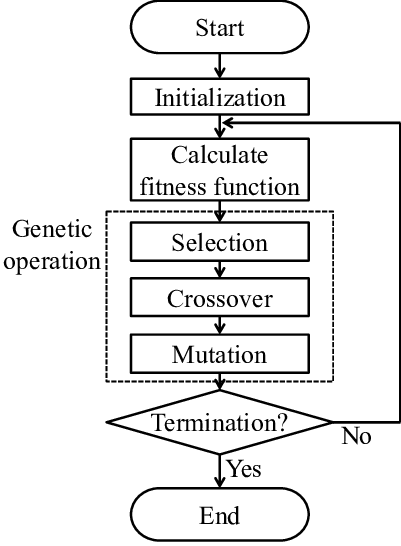
\includegraphics[width=0.3\linewidth]{genalgooutilne.png}
    \caption{General outline of genetic algorithm \parencite{gaoutline}}
    \label{fig:GAoutline}
\end{figure}
Genetic Algorithms are often used for complex optimization problems that may involve large search spaces with multiple best candidate solutions, where using traditional gradient-based methods or simple brute force may take up much higher computation power and time. Layout optimization problems fall into this category, as they typically involve combinatorial decision variables, geometric constraints, and multiple feasible solutions or configurations. In the context of the design of a robotic workcell layout, each chromosome can represent a complete spatial configuration of machines, including their positions and orientations within a workspace. The evolutionary process then explores different layout configurations to minimize a defined objective, in our case, the fitness function, which is primarily the total robot travel distance. It is also important to note that the fitness function in this current study is favored to be minimized, as a lower robot travel distance is more favorable.

Another key advantage of GA is its population-based search strategy, which allows simultaneous exploration of multiple regions of the search space. This characteristic reduces the likelihood of premature convergence to a local optima, which is a widely known common challenge in evolutionary algorithms. Furthermore, GA operators can be easily adapted to adhere to domain-specific constraints, such as collision avoidance, workspace boundaries, and machine accessibility issues.

\subsection{Local Search}
Local search is commonly integrated with Genetic Algorithms (GA) to improve the fitness of the best candidate solutions (elites) during the evolutionary process. In classical GA, mutation and crossover introduce diversity into the population, however, these operators alone may not efficiently refine promising solutions once the search approaches high-quality of candidates of solutions in the population space. Local search addresses this limitation by performing additional mutations or modifications on selected individuals, typically the best-performing solutions in the population \parencite{talbi2009metaheuristics}. This is an efficient strategy to escape local optima, since local search typically is applied as exploitation to offsprings from crossover, and unlike mutation, it only accepts modifications that generate better fitness.

Local search modifies the candidate solutions through mutation or neighborhood exploration and accepts the modification if it produces an improvement in fitness, unlike mutation which does not evaluate the improvement in fitness. This process enables the algorithm to perform a more intensive search within the regions of the solution space, therefore increasing the likelihood of discovering higher-quality solutions \parencite{blum2003metaheuristics}. Such hybridization of global evolutionary search with local improvement strategies is often referred to as a \textit{memetic algorithm}, which combines population-based exploration with individual-level exploitation \parencite{moscato1989memetic}.

While local search can significantly improve solution quality, it introduces an additional computational cost. Each local improvement step requires evaluating neighboring solutions, which increases the total runtime of the algorithm. Consequently, frequent application of local search may lead to substantially higher computational time, particularly for complex optimization problems with expensive fitness evaluations. For this reason, many implementations apply local search selectively, for example only to a small number of candidate solutions or with a smaller probability, in order to balance solution improvement and computational efficiency \parencite{talbi2009metaheuristics}.

\subsection{Limitations of Static Parameter Configuration in Genetic Algorithms}

Although the GA framework developed by \textcite{sim2005rwl} demonstrated strong performance, the algorithm used fixed parameter settings for the mutation rate, crossover rate, and elitism. These static parameter configurations are common in classical GA implementations. According to \textcite{goldberg1989genetic}, the performance of genetic algorithms is highly dependent on the choice of parameters. For example, premature convergence might be caused due to low mutation and high elitism, where the population becomes similar too quickly, making GA stuck in a local optimum.

\textcite{eiben1999parametercontrol} categorized parameter control in evolutionary algorithms into deterministic, adaptive, and self-adaptive approaches, emphasizing that optimal parameter settings are rarely constant across generations. \textcite{eiben1999parametercontrol} changed GA parameters such as mutation and crossover by observing the conditions simply through if-else blocks. This study is then supported from the study of \textcite{karafotias2015trends}, highlighting that fixed parameter tuning often limits robustness and generalization across different problem instances.

In robotic workcell layout optimization, this limitation becomes significant because the search landscape evolves dynamically. Early generations benefit from exploration to sample diverse spatial configurations, whereas later generations require exploitation to refine promising layouts. Static mutation and crossover rates assume a stationary search environment, which contradicts the inherently dynamic behavior of evolutionary processes.

Therefore, while the GA formulation by \textcite{sim2005rwl} provides a strong structural foundation, its optimization performance may be further improved through adaptive parameter control.

\subsection{Initialization Improvements versus Dynamic Adaptation}

Recent research has enhanced GA performance by improving initialization strategies. For instance, \textcite{abwahab2024eswa} introduced a fitness-guided initialization mechanism for mobile robot path planning, improving early convergence and reducing infeasible solutions. \textcite{ruan2024tsp} integrated GA and RL using a Double Q-Learning algorithm to solve the Traveling Salesman Problem (TSP). The TSP seeks the shortest route that visits each city exactly once, a formulation closely analogous to the robotic workcell optimization problem. However, \textcite{ruan2024tsp} only optimized the initial population generation, while the GA parameters remained static.

While population initialization improves the early phase of evolution, they do not explicitly address the evolving nature of parameter effectiveness across generations, since the parameters still remain static. Better initialization may serve as a better \textit{headstart} to achieve faster convergence, however, even with high-quality initial solutions, fixed mutation and crossover rates may still lead to premature convergence in later generations of the search. 

Therefore, as explained in Section 2.3, adaptive parameter control can potentially provide more impactful improvements compared to initialization-based enhancements. While improved initialization strategies mainly affect the early exploration phase of the search, adaptive parameter control influences the entire evolutionary process by adjusting algorithm behavior according to the current search dynamics. Another thing to consider for future studies, is that these two approaches address different aspects of the optimization process, they are independent towards each other and can be integrated within the same framework to further enhance optimization performance. However, this paper focuses more on using a model that dynamically adapts the parameters, instead of improving the initial population.

\subsection{Exploration and Exploitation in Evolutionary Algorithms}
A fundamental challenge in evolutionary optimization is maintaining a balance between \textit{exploration} and \textit{exploitation}. Exploration refers to the ability of the algorithm to investigate diverse regions of the search space, while exploitation focuses on refining promising candidate solutions to improve fitness. Achieving an appropriate balance between these two behaviors is critical for avoiding premature convergence while still enabling efficient optimization and search for better solutions with different characteristics through exploration \parencite{eiben1999parametercontrol}.

In GA, exploration is usually introduced through stochastic operators such as mutation and crossover, which generate new candidate solutions and increase population diversity. These mechanisms enable the algorithm to discover previously unexplored regions of the search space. On the other hand, exploitation is achieved through selection and local search on offsprings, where better fitness candidate solutions or offsprings are cherry-picked and each modified in a way that improves fitness, to the next generations, allowing the algorithm to refine through crossover and repeat local search for promising solutions over time \parencite{goldberg1989genetic}.

An excessive usage on exploration may cause the algorithm to behave similarly to random search, which may slow convergence toward optimal solutions. On the other hand, excessive exploitation usage can cause the population to become too homogeneous, leading to premature convergence in suboptimal regions of the search space, where the algorithm fails to look through other characteristics of solutions which can be a better solution candidate. Therefore, evolutionary algorithms must dynamically balance these competing objectives throughout the optimization process \parencite{back1996evolutionary}.

In practice, the exploration–exploitation balance evolves naturally during the course of an evolutionary run. Early generations typically benefit from greater exploration to sample diverse regions of the search space, while later generations require stronger exploitation to refine promising solutions. However, fixed algorithm parameters such as static mutation and crossover rates cannot fully accommodate this changing requirement. As a result, adaptive parameter control mechanisms have been proposed to dynamically regulate the balance between exploration and exploitation during the evolutionary process \parencite{eiben1999parametercontrol}.

This dynamic perspective motivates the integration of learning-based control mechanisms within evolutionary algorithms. By observing population statistics such as diversity and fitness improvement, a learning agent can learn the current generation state and adjust algorithm parameters to regulate exploration and exploitation more effectively during different stages of the search process.

\subsection{Reinforcement Learning for Self-Adaptive Parameter Control}
Reinforcement Learning (RL) provides a principled framework for sequential decision-making in dynamic environments \parencite{sutton2018reinforcement}. In RL, an agent observes the state of an environment, selects an action, receives a reward, and updates its policy to maximize long-term cumulative reward, as shown in Figure \ref{fig:rlagent}. 
\begin{figure}[H]
    \centering
    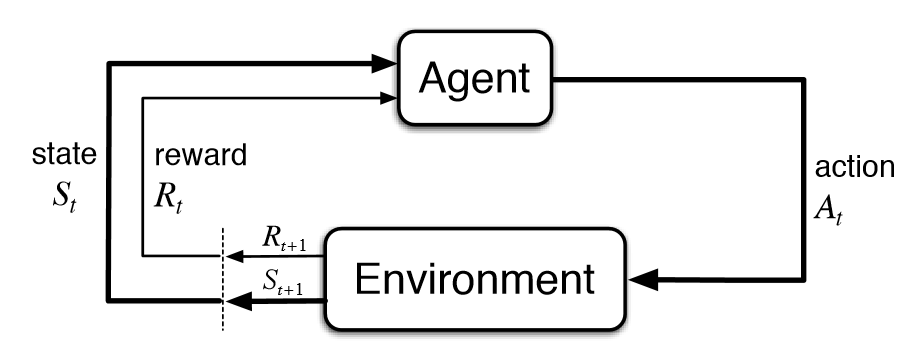
\includegraphics[width=0.5\linewidth]{references pic/RLPic_SuttonBarto.png}
    \caption{Reinforcement Learning agent and its environment interactions flowchart \parencite{sutton2018reinforcement}}
    \label{fig:rlagent}
\end{figure}
The GA evolutionary process can be formulated as a Markov Decision Process (MDP):
\begin{itemize}
    \item \textbf{State:} Population metrics such as diversity and fitness improvement.
    \item \textbf{Action:} Adjustment of GA parameters (mutation rate scaling, crossover rate modification, mutation strategy selection, local search activation).
    \item \textbf{Reward:} Improvement in fitness between consecutive generations.
\end{itemize}

A key idea in value-based reinforcement learning is \textit{temporal-difference (TD) learning}, which was introduced by \textcite{sutton1988td} as a methodology for prediction through incremental learning, where value estimates are updated based on the difference between successive state evaluations. Given a state $S_t$, the estimated value $V(S_t)$ is updated as

\begin{equation}
    V(S_t) \leftarrow V(S_t) + \alpha \left[ V(S_{t+1}) - V(S_t) \right]
    \label{eq:rlupdaterule}
\end{equation}
where $\alpha$ is the learning rate controlling the step size of the update. Equation \ref{eq:rlupdaterule} allows the agent to continuously refine and update its value estimates based on observed transitions between states.

Generally, to maximize returns, agents often selects actions greedily by choosing the action that leads to the highest estimated value or reward. However, greedy behavior can potentially lead to premature convergence due to the lack of exploration, or trial and error policies. Hence, exploration strategies such as $\epsilon$-greedy policies allow the agent to occasionally, in this paper, select random actions to discover for more optimum solutions, whether during exploration or escaping local optima at later generations. The $\epsilon$ parameter defines the chance of choosing random actions, which typically is set at smaller values.

This exploration principle is particularly important when applying RL to evolutionary algorithms. Unlike deterministic environments such as board games, genetic algorithms inherently rely on stochastic search processes. Excessive greedy parameter selection (high exploitation) could quickly reduce population diversity and lead to premature convergence. Therefore, an RL agent is proposed in this study to maintain a degree of exploration and exploitation when adjusting the algorithm parameters for the sake of producing a better quality solution for robotic workcell layout problems.

Recent studies have researched on the effectiveness of RL compared to traditional GA that might support this approach. \textcite{quevedo2021gecco} applied RL to dynamically tune GA parameters for vehicle routing problems, where the solutions obtained by RL-GA were better for up to 11\% improvement. Meanwhile, \textcite{Woodcock2024Genetic} proposed a RL-GA Q-learning agent to optimize mutation rates, where the agent learnt to select high mutation rates when the variance or diversity were too low, leading to better fitness returns.

These findings ultimately serve as strong motivations to implement RL as a theoretically sound and empirically validated mechanism to improve adaptive hyperparameter control in enhancing genetic algorithms, where it would be applied to solve for the robotic workcell layout problem as a novel approach.

\subsection{Positioning of the Present Study}

Building upon the GA-based robotic workcell layout formulation introduced by \textcite{sim2005rwl}, this study worked on enhancing the optimization framework by enforcing a Reinforcement Learning (RL) agent to control the parameter's of the GA process. Rather than improving the initial population and fitness formulation, this research's scope is to look for a novel approach by introducing a reinforcement learning - genetic algorithm (RL-GA) agent for GA adaptive parameter control to solve for 2D robotic workcell layout problems, bridging the gap between adaptive GA parameter control and the optimization of the robotic workcell layout. Tests and comparisons were kept fair to compare with the same initial population throughout this paper. Specifically, the proposed framework dynamically adjusts mutation rates, crossover rates, mutation strategies, and local search activation based on population diversity and fitness improvement bins. 

\newpage
\section{Data Classes}
This project adopted Python’s dataclass wrapper to define the geometric and physical constraints of the machines and workcell layout in this problem. It maintains the integration of RL with GA through collision detection for feasible solutions, and visualization functions to analyze optimized robotic workcell layouts.  The dataclass would define the physical layout representation and also the decoded machine geometry, global location, coordinates and rotation configurations. Last but not least, these were also used to easily visualize the physical layout and evaluation later on.

\subsection{Point}
The Point dataclass represents a two-dimensional Cartesian coordinate and serves as the fundamental geometric vertice within the system. It is used to describe machine positions, access points, robot starting locations, and polygon vertices. The dataclass stores the coordinates $(x, y)$ and provides a method for computing Euclidean distance between two points, which is essential for evaluating robot travel distance within the fitness function. An example of the usage of the Point dataclass is the position of the robot in the workcell layout, which is always kept constant at Point(0, 0), e.g. the origin of the layout.

\subsection{Machine}
The Machine dataclass represents a physical workstation in the robotic workcell. It stores both geometric properties and operational interaction points, allowing the optimization algorithms to be aware of the constraints for a physical workstation, especially when solutions are not feasible due to collision. The Machine dataclass also supports modifications for other kinds of machine shapes, making it reusable for other experiments. In this paper, however, only rectangular and L-shaped machines are used.

Each machine could be defined by these data members:
\begin{itemize}
    \item A unique identifier,
    \item A geometric shape (rectangular or L-shaped),
    \item Physical dimensions (width and height for rectangular, addition of width and height cut out for L-shaped),
    \item A local access point relative to the machine center,
    \item A global position and rotation angle.
\end{itemize}
When defining the machine, the global position and rotation angle were not set as these would be handled by GA during its creation of the initial population phase, where the chromosomes would then be decoded and assigned to the global position and rotation angle data member.

\subsubsection{Shape Abstraction}

Both rectangular and L-shaped machines are represented using a unified dataclass. Shape-specific geometry is handled internally within the dataclass methods, rather than through external conditional logic. This approach simplifies integration with optimization, collision detection, and visualization modules, while allowing for straightforward extension to additional machine geometries.

\begin{figure}[htbp]
\centering
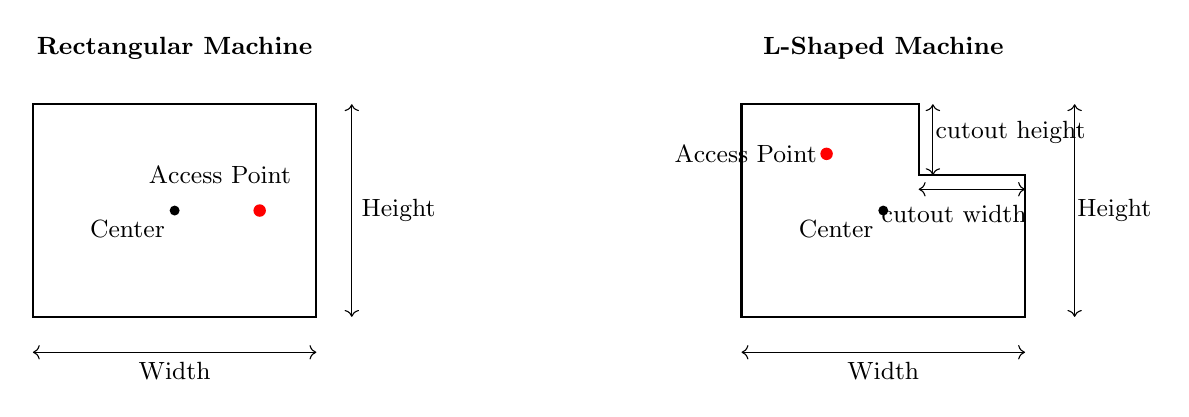
\begin{tikzpicture}[scale=0.9, every node/.style={font=\small}]

% =========================
% RECTANGULAR MACHINE
% =========================
\begin{scope}[shift={(-5,0)}]

% Rectangle
\draw[thick] (-2,-1.5) rectangle (2,1.5);

% Center
\fill (0,0) circle (2pt);
\node[below left] at (0,0) {Center};

% Width and Height
\draw[<->] (-2,-2) -- (2,-2);
\node[below] at (0,-2) {Width};

\draw[<->] (2.5,-1.5) -- (2.5,1.5);
\node[right] at (2.5,0) {Height};

% Access Point
\fill[red] (1.2,0) circle (2.5pt);
\node[right] at (-0.5,0.5) {Access Point};

% Label
\node[above] at (0,2) {\textbf{Rectangular Machine}};

\end{scope}

% =========================
% L-SHAPED MACHINE
% =========================
\begin{scope}[shift={(5,0)}]

% L-shape outline
\draw[thick]
(-2,-1.5) --
(2,-1.5) --
(2,0.5) --
(0.5,0.5) --
(0.5,1.5) --
(-2,1.5) -- cycle;

% Center
\fill (0,0) circle (2pt);
\node[below left] at (0,0) {Center};

% Overall Width
\draw[<->] (-2,-2) -- (2,-2);
\node[below] at (0,-2) {Width};

% Overall Height
\draw[<->] (2.7,-1.5) -- (2.7,1.5);
\node[right] at (2.6,0) {Height};

% Cutout Width
\draw[<->] (0.5,0.3) -- (2,0.3);
\node[above] at (1, -0.3) {cutout width};

% Cutout Height
\draw[<->] (0.7,0.5) -- (0.7,1.5);
\node[right] at (0.6,1.1) {cutout height};

% Access Point
\fill[red] (-0.8,0.8) circle (2.5pt);
\node[left] at (-0.8,0.8) {Access Point};

% Label
\node[above] at (0,2) {\textbf{L-Shaped Machine}};

\end{scope}

\end{tikzpicture}
\caption{Examples of geometric definition of rectangular and L-shaped machines. 
The machines' points are defined relative to their center position, with dimensions, rotation (not shown), and a local access point that is transformed into world coordinates.}
\label{fig:machine_geometry}
\end{figure}

\subsubsection{World Coordinate Transformation}

Two key functions are implemented within the Machine dataclass:

\begin{itemize}
    \item Computing the polygon vertices of the machine in world coordinates by applying rotation and translation,
    \item Transforming the machine's local access point into global coordinates.
\end{itemize}

These transformations provide a mapping or translation from chromosome variables to physical geometry in world coordinates for each of the machines or workstations involved. This logic ensures that collision detection, distance computation, and visualization operate on physically feasible solutions.

\newpage
\section{Collision Detector}

Collision detector is a class that consists of multiple test functions to ensure that machines placed within the robotic workcell do not overlap or collide in physical space. Since machines are represented as polygons (rectangular or L-shaped), the problem reduces to determining whether two simple polygons intersect in a two-dimensional plane. This project implements collision detection using classical computational geometry techniques, including point-in-polygon testing and line segment intersection analysis.

\subsection{Point-in-Polygon Test}
The function determines whether a given point lies inside a polygon using the ray casting algorithm. A horizontal ray is cast from the query point to the positive $x$-direction, and the number of times this ray intersects the polygon edges is counted. If the number of intersections is odd, the point lies inside the polygon; if even, it lies outside.
\begin{figure}[H]
    \centering
    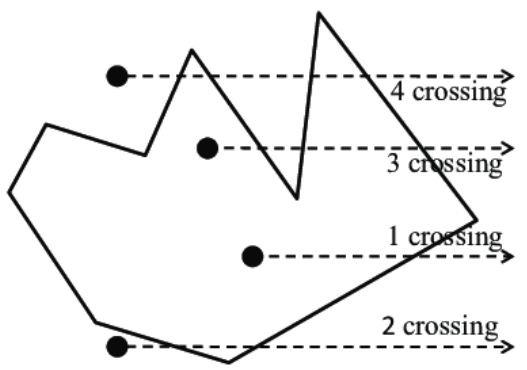
\includegraphics[width=0.3\linewidth]{raycasting.png}
    \caption{Sample illustration of ray casting algorithm on a polygon \parencite{raycasting}}
    \label{fig:placeholder}
\end{figure}
For each polygon edge defined by vertices $(x_1, y_1)$ and $(x_2, y_2)$, an intersection occurs if:
\begin{itemize}
    \item The point's $y$-coordinate lies within the vertical range of the edge:
    \[
    y \in (\min(y_1, y_2), \max(y_1, y_2)]
    \]
    \item The $x$-coordinate of the ray intersection lies to the right of the point:
    \[
    x \le x_{\text{int}}
    \]
\end{itemize}

where the intersection $x$-coordinate is computed using linear interpolation in Equation \ref{eq:linearinterpolation}:
\begin{equation}
    x_{\text{int}} = x_1 + (y - y_1)\frac{x_2 - x_1}{y_2 - y_1}
    \label{eq:linearinterpolation}
\end{equation}

To avoid division by zero, horizontal edges are excluded from the intersection calculation, since horizontal edges have the same initial and final $y$ coordinates. This implementation is valid for simple polygons but may classify points lying exactly on polygon edges inconsistently, which is a known limitation of ray casting methods.

\subsection{Line Segment Intersection Test}
The function determines whether two line segments intersect using orientation tests, adapted directly from a forum in \textcite{geeksforgeeks_segment_intersection}'s \textit{How to check if two given lines intersect?}.

\begin{figure}[H]
    \centering
    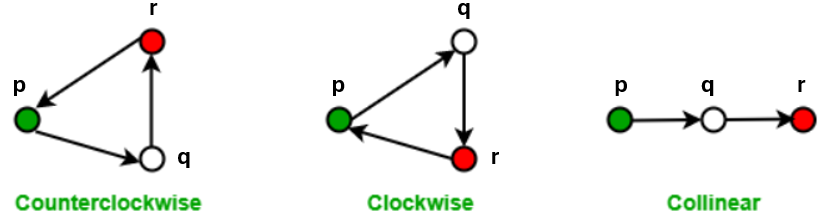
\includegraphics[width=0.5\linewidth]{lineintersect1.png}
    \caption{Possible orientations of three points p, q, and r \parencite{geeksforgeeks_segment_intersection}}
    \label{fig:placeholder}
\end{figure}

Given three points $p$, $q$, and $r$, the orientation is computed as:
\[
\text{val} = (q_y - p_y)(r_x - q_x) - (q_x - p_x)(r_y - q_y)
\]

The orientation is interpreted as:
\begin{itemize}
    \item $\text{val} = 0$: collinear
    \item $\text{val} > 0$: clockwise
    \item $\text{val} < 0$: counterclockwise
\end{itemize}

\begin{figure}[H]
    \centering
    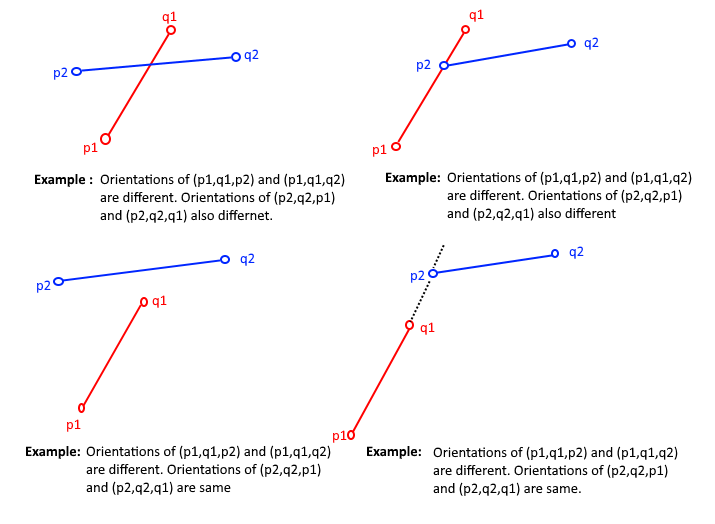
\includegraphics[width=0.6\linewidth]{lineintersect2.png}
    \caption{Different variations for general cases of two lines}
    \label{lineintersect2}
\end{figure}
Two segments $(p_1, q_1)$ and $(p_2, q_2)$ intersect in the general case if:
\[
\text{orient}(p_1, q_1, p_2) \ne \text{orient}(p_1, q_1, q_2)
\quad \text{and} \quad
\text{orient}(p_2, q_2, p_1) \ne \text{orient}(p_2, q_2, q_1)
\]
as shown in Figure \ref{lineintersect2}.

\begin{figure}[H]
    \centering
    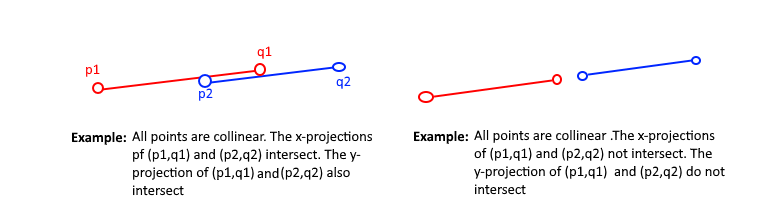
\includegraphics[width=0.6\linewidth]{lineintersect3.png}
    \caption{Special cases for collinear lines}
    \label{lineintersect3}
\end{figure}
Special cases are handled when points are collinear by checking whether one point lies within or on the edge of the other segment, as shown in Figure \ref{lineintersect3}.

\subsection{Polygon Intersection Test}
This function determines whether two polygons intersect by combining three checks:
\begin{enumerate}
    \item Any vertex of the first polygon lies inside the second polygon,
    \item Any vertex of the second polygon lies inside the first polygon,
    \item Any edge of the first polygon intersects any edge of the second polygon.
\end{enumerate}

If any of these conditions are satisfied, the polygons are considered to be intersecting, and hence not a valid layout configuration.

This composite approach is effective for detecting collisions between simple polygons and is commonly used in practical applications. It correctly identifies both containment-based intersections and edge-crossing intersections.

\newpage
\section{Helper Functions}
\subsection{Total Distance Calculation}
This function computes the total travel distance of the robot for a given layout configuration. The robot starts from a fixed initial position and visits machines according to a predefined processing sequence. For each machine ID in the sequence, the corresponding machine is identified and its access point in world coordinates is appended to the path. The total distance is then obtained by summing the Euclidean distances between consecutive positions along this path. Since the sequence is fixed, the resulting distance depends solely on the spatial arrangement of the machines.

Let $p_0$ denote the robot's initial position, and let $p_i$ denote the world-coordinate access point of machine $i$ in the processing sequence. If the sequence contains $N$ machines, the total robot travel distance is defined in Equation \ref{eq:dtraveleqn}:

\begin{equation}
D_{\text{travel}} =
\sum_{i=0}^{N}
\left\| p_i - p_{i+1} \right\|_2
\label{eq:dtraveleqn}
\end{equation}

represents the return to the robot's starting position. The Euclidean distance between two points $p_i = (x_i, y_i)$ and $p_j = (x_j, y_j)$ is defined in Equation \ref{eq:eucliddistance}:

\begin{equation}
\left\| p_i - p_j \right\|_2
=
\sqrt{(x_i - x_j)^2 + (y_i - y_j)^2}
\label{eq:eucliddistance}
\end{equation}

\subsection{Collision Checker}
Collision detection is performed by checking for geometric intersections between all pairs of machines. Each machine is represented as a polygon defined by its corner points. A nested loop iterates over all unique machine pairs, and the final collision verdict is obtained the CollisionDetector class. This method determines whether two polygons overlap or intersect. If any collision is detected, the function immediately returns True and the fitness of the particular layout is set to $\infty$; otherwise, it returns False after all pairs and fitness have been evaluated, which will be explained in the upcoming sections.

\subsection{Workspace Bounds}
This function ensures that all machines remain fully within the predefined workspace boundaries. For each machine, all corner points are evaluated against the workspace limits in both the \(x\)- and \(y\)-directions. If any corner lies outside the allowable region, the layout is considered invalid and the function returns False. A layout is only accepted if every machine is entirely contained within the workspace. The workspace boundaries set for all problems across this paper is (-15, 15, -15, 15), i.e. a square with sides of 30 units, with its center located at the origin.

\newpage
\section{Genetic Algorithm}

This section describes the Genetic Algorithm (GA) framework employed for robotic workcell layout optimization. GA searches for the optimal machine placements and orientations within a bounded workspace while minimizing robot travel distance and satisfying geometric feasibility constraints. GA operators such as elitism, tournament selection, crossover, and mutation
follow the classical genetic algorithm framework described by
\textcite{goldberg1989genetic}. The integration of local search is inspired by the concept of \textit{memetic algorithms} introduced by
\textcite{moscato1989memetic}, which combine evolutionary search with local improvement procedures. This hybridization between global evolutionary search and local exploitation has since been widely applied in metaheuristic optimization frameworks \parencite{talbi2009metaheuristics}.

\subsection{Initialization}

The genetic algorithm is initialized with a predefined set of machines, a fixed processing sequence, the robot start position (layout origin), and rectangular workspace boundaries. Each machine is characterized by its geometry, access point, and allowable rotations. The algorithm operates with a fixed population size and a predefined number of generations. In this study, the default parameters are:
\begin{itemize}
    \item Population size = 200
    \item Number of generations = 300
    \item Mutation rate = 10\%
    \item Crossover rate = 80\%
    \item Elitism rate = 10\%
    \item Local search rate = 10\%
\end{itemize}

Performance metrics such as best fitness and average fitness are recorded at each generation to analyze convergence behavior.

\subsection{Chromosome Representation}

Each candidate solution, referred to as a chromosome, encodes a complete layout of all machines in the workcell. For a system consisting of $N$ machines, each machine $i$ is represented by a triplet:
\[
(x_i, y_i, \theta_i),
\]
where $(x_i, y_i)$ denotes the machine center position and $\theta_i$ denotes its rotation angle.

The full chromosome is therefore defined as a vector:
\[
\mathbf{c} = [x_1, y_1, \theta_1, \dots, x_N, y_N, \theta_N].
\]

To reflect practical layout constraints, rotational values are discretized to the nearest multiple of $90^\circ$, i.e., $\{0^\circ, 90^\circ, 180^\circ, 270^\circ\}$. This model also supports for custom machine rotation if practical constrains are neglected.

Rather than encoding the layout into series of bits (0s and 1s), which are very common in traditional genetic algorithm papers, such as implementations done by \textcite{sim2005rwl}, this research utilizes a more visible and inferable chromosome representation to ease debugging, analyzing machine configurations with overall a better physical understanding regarding what GA does to the machines. Hence, although this does not fully follow traditional GA chromosome encoding methods, this method is entirely inspired by GA itself.
\subsection{Creating the Initial Population}
\begin{algorithm}[H]
\caption{Initial Population Generation}
\label{alg:init_population}
\begin{algorithmic}[1]
\Require Machines $\mathcal{M}$, workspace bounds $\mathcal{B}$, population size $P$
\Ensure Population of chromosomes $Population$

\State $Population \gets \emptyset$

\For{$i = 1$ to $P$}
    \State $Chromosome \gets [\ ]$
    
    \For{each machine $m_j \in \mathcal{M}$}
        \State Randomly sample position $(x_j, y_j)$ within workspace bounds
        \State Randomly sample rotation $\theta_j \in [0, 360)$
        \State Append $(x_j, y_j, \theta_j)$ to $Chromosome$
    \EndFor
    
    \State Add $Chromosome$ to $Population$
\EndFor

\State \Return $Population$
\end{algorithmic}
\end{algorithm}
The initial population is generated by randomly sampling machine positions and orientations within the workspace boundaries. To promote spatial diversity and reduce early-stage collisions, machines are preferentially distributed across four workspace quadrants when possible. Remaining machines are placed uniformly within the allowable region.

This initialization strategy encourages a diverse set of feasible starting layouts, improving early exploration of the search space.

\subsection{Decoding Chromosomes}

Each chromosome is decoded into a list of machine configurations by mapping gene triplets to machine positions and orientations. Rotational values are discretized to the nearest multiple of $90^\circ$. The decoded layouts are subsequently used for collision detection, workspace boundary validation, and fitness evaluation.

\subsection{Fitness Calculation}

The fitness function evaluates each chromosome based on both hard feasibility constraints and soft optimization objectives. Since lower distance, as a primary metric in fitness calculation, means better solution, lower fitness hence means better fitness in this task.

\subsubsection{Hard Constraints}

A chromosome is assigned an infinite fitness value if any of the following constraints are violated:
\begin{itemize}
    \item Any machine overlaps the robot start position.
    \item Any two machines geometrically intersect.
    \item Any machine extends beyond the workspace boundaries.
\end{itemize}

These constraints ensure that only physically feasible layouts are considered during optimization.

\subsubsection{Fitness Function}
For feasible layouts, the fitness function is defined in Equation \ref{eq:fitnessfunction}:
\begin{equation}
    f = D_{\text{travel}} + P_{\text{compactness}} - B_{\text{accessibility}}
    \label{eq:fitnessfunction}
\end{equation}
where:
\begin{itemize}
    \item $D_{\text{travel}}$ is the total robot travel distance,
    \item $P_{\text{compactness}}$ penalizes spatially spread layouts,
    \item $B_{\text{accessibility}}$ rewards layouts with improved access clearance.
\end{itemize}

The robot travel distance ($D_{\text{travel}}$) is computed as the total Euclidean distance starting at the robot base, see Equation \ref{eq:dtraveleqn}, where the machine access points are visited in a predefined sequence, which then returns to the base.

Compactness refers to the degree to which machines are arranged within a limited spatial area of the workspace. In real life engineering problems, compactness is often more favorable to reduce unnecessary spatial spread of equipment while maintaining accessibility and operational feasibility \parencite{tompkins2010facilities}. In this study, compactness is defined as a penalty proportional to the spatial span of machine centers along the horizontal and vertical directions.

Compactness is set in Equation \ref{eq:compactess} by penalizing the spatial span of machine centers:
\begin{equation}
    P_{\text{compactness}} = \beta \left( x_{\text{span}} + y_{\text{span}} \right)
    \label{eq:compactess}
\end{equation}
where:
\begin{itemize}
    \item $P_{\text{compactness}}$ is the compactness penalty.
    \item $\beta = 0.1$ is the compactness scaling coefficient.
    \item $x_{\text{span}} = \max_i(x_i) - \min_i(x_i)$ is the horizontal span of the layout.
    \item $y_{\text{span}} = \max_i(y_i) - \min_i(y_i)$ is the vertical span of the layout.
\end{itemize}
\begin{figure}[H]
    \centering
    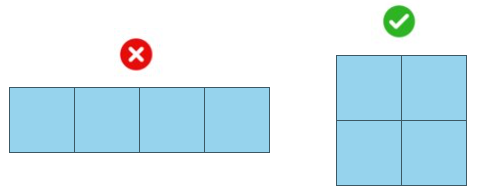
\includegraphics[width=0.5\linewidth]{compactnesspenalty.png}
    \caption{An example of better compactness configuration, where machine placements with lesser spans (right) are more favored.}
    \label{fig:compactnessexample}
\end{figure}
Figure \ref{fig:compactnessexample} shows two different scenarios of machine placements, where a more compact machine is more favorable as it reduces the penalty, which contributes for better fitness. The compactness scaling coefficient $\beta$ is chosen as 0.1 to add a complimentary feature to the fitness function, as the main contributor of the fitness function would still be the robot travel distance.

Accessibility is quantified by measuring clearance around machine access points. It is generally not favorable for machines to be too close or compact to each other, making it impossible to recreate in real life scenarios. For each machine, the minimum distance from its access point to neighboring machine corners is computed and aggregated to form the accessibility bonus, see Figure \ref{fig:accessibilityexample}. The accessibility bonus is defined in Equation \ref{eq:bonusaccessibility} as

\begin{equation}
B_{\text{accessibility}} = \alpha \sum_{i=1}^{N} \left( \min_{\substack{j \neq i \\ c \in C_j}} \|A_i - c\|_2 \right)
\label{eq:bonusaccessibility}
\end{equation}

where:
\begin{itemize}
    \item $B_{\text{acc}}$ is the accessibility bonus.
    \item $\alpha = 0.05$ is the scaling coefficient.
    \item $N$ is the number of machines.
    \item $A_i$ is the world-coordinate access point of machine $i$.
    \item $C_j$ is the set of corner points of machine $j$.
    \item $\lVert \cdot \rVert_2$ denotes the Euclidean distance.
\end{itemize}
\begin{figure}[H]
    \centering
    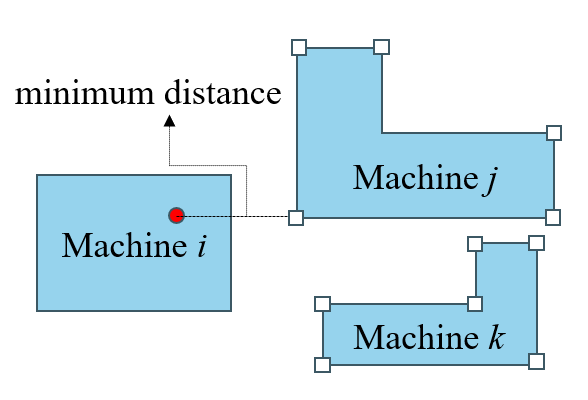
\includegraphics[width=0.5\linewidth]{accessibilitybonus.png}
    \caption{An example of minimum Euclidean distance chosen for a machine, this calculation repeats for every other machines, which are then summed and multiplied by a scaling coefficient $\alpha$.}
    \label{fig:accessibilityexample}
\end{figure}
This metric is of opposite nature when finding for the shortest robot travel distance. In real life engineering applications, machines are primarily placed with gaps, instead of cramming them until no space is left in between. This metric hence acts as a soft collision buffer and fitness feature, hence the low $\alpha$ value, in order to encourage optimized layouts to reduce crowding and better reachability for robots or humans.

In case of invalid layouts generated during crossover or mutation, their fitness scores are assigned as an infinite fitness value. This ensures that infeasible solutions are unlikely to be selected for reproduction in subsequent generations. For future purposes, the fitness function can be modified according to the user's interest if necessary, as this paper only shows the base or template fitness function for this problem.

\subsection{Elitism}
Elitism preserves a fixed portion of the best-performing chromosomes between generations. These elite individuals are copied unchanged into the next generation, ensuring that high-quality solutions are not lost due to stochastic genetic operations. Although elites are not modified through any GA operators, for each generations, the candidate solutions in the population are sorted, which could indirectly replace the top \% elites if a better solution is found. This ensures that for increasing iterations in generations, the best solution would never degrade, it would either stay the same or improve. The elitism rate is kept constant as 10\% of the population size throughout each generations.
\subsection{Tournament Selection}
\begin{algorithm}[H]
\caption{Tournament Selection}
\label{alg:tournament}
\begin{algorithmic}[1]
\Require Population $P$, fitness values $F$, tournament size $k$
\Ensure Selected parent chromosome

\State Randomly select $k$ individuals from $P$
\State Retrieve their corresponding fitness values
\State Identify the individual with the minimum fitness
\State Return a copy of the selected chromosome

\end{algorithmic}
\end{algorithm}
Parent selection is performed using tournament selection. A subset of individuals is randomly sampled from the population, and the chromosome with the lowest fitness value is selected as a parent. This approach maintains strong selection pressure toward high-quality solutions while preserving diversity by allowing weaker individuals a chance to be selected.

\subsection{Crossover}
\begin{algorithm}[H]
\caption{Uniform Crossover}
\label{alg:crossover}
\begin{algorithmic}[1]
\Require Parent chromosomes $p_1$, $p_2$, crossover rate $p_c$
\Ensure Offspring chromosomes $c_1$, $c_2$

\If{random number $> p_c$}
    \State \Return copies of $p_1$ and $p_2$
\EndIf

\State $c_1 \gets p_1$, $c_2 \gets p_2$

\For{each gene index $i$}
    \If{random number $< 0.5$}
        \State swap $c_1[i]$ and $c_2[i]$
    \EndIf
\EndFor

\State \Return $c_1, c_2$
\end{algorithmic}
\end{algorithm}
Uniform crossover is applied to selected parent chromosomes with probability $p_c$. For each gene position, the offspring inherits the gene from either parent with equal probability. If crossover is not triggered, both parents are copied directly into the offspring population. This operator enables flexible recombination of spatial and rotational information.

\subsection{Mutation}
\begin{algorithm}[H]
\caption{Mutation}
\label{alg:mutation}
\begin{algorithmic}[1]
\Require Chromosome $c$, mutation rate $p_m$, workspace bounds $\mathcal{B}$
\Ensure Mutated chromosome $c'$

\State $c' \gets$ copy of $c$

\For{each machine gene triplet $(x_i, y_i, \theta_i)$ in $c'$}
    \If{random number $< p_m$}
        \State $x_i \gets x_i + \mathcal{N}(0, \sigma_p)$
        \State $y_i \gets y_i + \mathcal{N}(0, \sigma_p)$
        \State $\theta_i \gets$ random choice from $\{0^\circ,90^\circ,180^\circ,270^\circ\}$
        \State Clip $(x_i,y_i)$ to workspace bounds
    \EndIf
\EndFor

\State \Return $c'$
\end{algorithmic}
\end{algorithm}
Mutation serves as the primary exploration mechanism in GA. It introduces stochastic modification to maintain genetic diversity and explore for better solutions, especially during the early stages of GA. For each machine, positional genes are modified using Gaussian noise, while rotational genes are reassigned to one of the four allowable discrete orientations. Machine positions are mutated by adding Gaussian-distributed modification with zero mean, allowing machines to move in any direction. For a machine $i$, the mutated coordinates are computed through Equation \ref{eq:mutationcoordinates}.
\begin{equation}
x_i' = x_i + \mathcal{N}(0, \sigma_p^2), \qquad
y_i' = y_i + \mathcal{N}(0, \sigma_p^2)
\label{eq:mutationcoordinates}
\end{equation}
where
\begin{itemize}
    \item $x_i, y_i$ are the original coordinates of machine $i$.
    \item $x_i', y_i'$ are the mutated coordinates.
    \item $\mathcal{N}(0, \sigma_p^2)$ denotes a Gaussian distribution with mean $0$ and standard deviation $\sigma_p=2.0$, i.e. variance $\sigma_p^2 = 2.0^2$.
\end{itemize}
Following normal distribution, the probability of the mutation step size to be $\pm$ 2.0 units is 68\%. Since Gaussian normal distribution is symmetric, the empirical rule deduces that the probability of the mutation step size of $>$ 2.0 units is 32\%.
After mutation, all machine positions are clipped to ensure compliance with workspace boundaries while accounting for individual machine dimensions.

\subsection{Local Search}
\begin{algorithm}[H]
\caption{Local Search}
\label{alg:local_search}
\begin{algorithmic}[1]
\Require Chromosome $c$, maximum iterations $T$
\Ensure Locally improved chromosome $c^\star$

\State $c^\star \gets c$
\State $f^\star \gets \Call{FitnessFunction}{c^\star}$

\For{$t = 1$ to $T$}
    \State $c' \gets$ copy of $c^\star$
    \State Randomly select one gene index

    \If{selected gene is a rotation gene}
        \State Apply a small random modification to the rotation
    \Else
        \State Apply a small random modification to the position
    \EndIf

    \State Evaluate $f' \gets \Call{FitnessFunction}{c'}$

    \If{$f' < f^\star$}
        \State $c^\star \gets c'$
        \State $f^\star \gets f'$
    \EndIf
\EndFor

\State \Return $c^\star$
\end{algorithmic}
\end{algorithm}
A hill-climbing local search is applied to a gene in a child chromosome generated crossover after tournament selection and previous mutations. In each local search iteration, a gene is modified by a small amount (Gaussian distribution), and the modification is accepted only if the fitness improves. This local refinement acts as an exploitation method by fine-tuning an offspring toward the nearest local optimum, which can complement the exploration that was done by mutation. During local search, it continuously applies random modification for a gene in a chromosome for a number of iterations. The number for maximum iterations of the local search is set to 5, which is constantly used throughout this research. In this standard GA, local search is applied to offspring generated by crossover. In the RL-GA framework described in the next section, local search is instead applied to elite chromosomes, which would further be discussed in the Discussion section.

\subsection{Default GA Parameter Values}

The default parameter settings used for the genetic algorithm in this study are summarized in Table \ref{tab:ga_parameters}. These default values are used for the experiments of standard GA and to train RL-GA Agent 2, which will be discussed during later sections.

\begin{table}[H]
\centering
\begin{tabular}{lc}
\toprule
\textbf{Parameter} & \textbf{Value} \\
\midrule
Population size & 200 \\
Number of generations & 300 \\
Mutation rate & 0.10 \\
Crossover rate & 0.80 \\
Elitism rate & 0.10 \\
\bottomrule
\end{tabular}
\caption{Default genetic algorithm parameters}
\label{tab:ga_parameters}
\end{table}
\vspace{-25pt}
The mutation rate default value of 0.10 and crossover rate of 0.80 were chosen to balance exploration and exploitation. According to \textcite{obitko1998ga} and \textcite{goldberg1989genetic}, mutation rate values are typically low around 0.01, however, to encourage for more exploration, this project increased the default mutation rate to 0.1. The typical crossover rate for GA is usually 0.7 - 0.9, where in this project the chosen default rate was 0.8. The elitism rate was chosen to be 0.1 to preserve high quality solutions and reduce execution time that might be used up for non-optimal solutions. The default population size and number of generations chosen would be supported in Chapters 8 and 11.
\subsection{Optimization Process}
\begin{figure}[H]
    \centering
    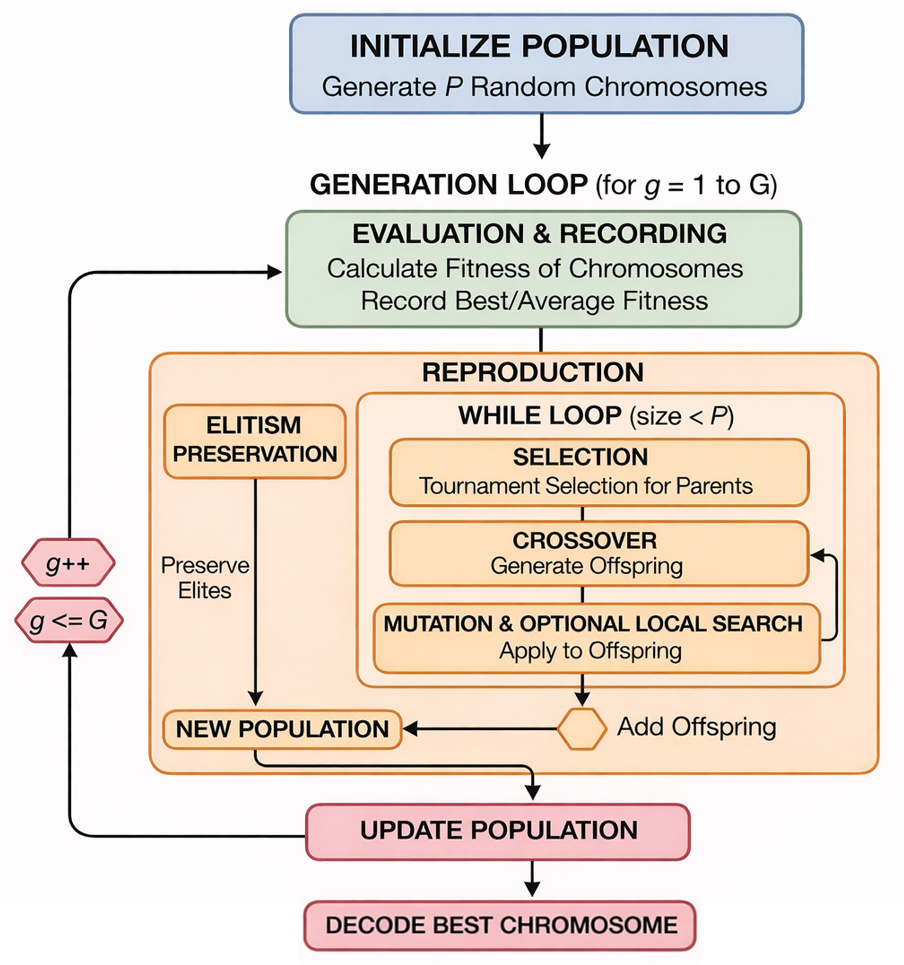
\includegraphics[width=0.7\linewidth]{standardGAdiagram.png}
    \caption{Standard Genetic Algorithm (GA) diagram for optimizing robotic workcell layout given population size of $P$ and generation size of $G$.}
    \label{fig:standardGAdiagram}
\end{figure}
% \begin{algorithm}[H]
% \caption{Genetic Algorithm for Robotic Workcell Layout Optimization}
% \label{alg:ga}
% \begin{algorithmic}[1]
% \Require Machines $\mathcal{M}$, processing sequence $\mathcal{S}$, workspace bounds $\mathcal{B}$, population size $P$, no. of generations $G$
% \Ensure Best layout $\mathcal{L}^\star$

% \State Initialize population $Population$ with $P$ random chromosomes
% \State $BestFitness \gets +\infty$

% \For{$g = 1$ to $G$}
%     \State Evaluate fitness of all chromosomes in $Population$
%     \State Record best and average fitness
    
%     \State Preserve elite individuals (elitism)
    
%     \State $NewPopulation \gets$ elites
    
%     \While{$|NewPopulation| < P$}
%         \State Select two parents using tournament selection
%         \State Generate offspring using crossover
%         \State Apply mutation to offspring and optionally apply local search
%         \State Add offspring to $NewPopulation$
%     \EndWhile
    
%     \State $Population \gets NewPopulation$
% \EndFor

% \State Decode best chromosome into machine layout $\mathcal{L}^\star$
% \State \Return $\mathcal{L}^\star$
% \end{algorithmic}
% \end{algorithm}
The optimization process proceeds iteratively across generations, as shown in Figure \ref{fig:standardGAdiagram}. During the while loop for each generations, the following steps are performed:
\begin{enumerate}
    \item Fitness evaluation of the current population.
    \item Preservation of elite solutions.
    \item Parent selection via tournament selection.
    \item Offspring generation through crossover and mutation.
    \item Optional local search refinement on offspring child (not elites), the refined chromosome replaces the original only if the fitness improves.
    \item Formation of the next generation.
\end{enumerate}

The algorithm finishes after a fixed number of generations and returns the best robotic workcell layout solution found during the GA search. In addition, fitness convergence histories and optimized layout snapshots are recorded for post-analysis and visualization.

\subsection{Summary}

The proposed standard GA framework is developed to solve the constrained robotic workcell layout optimization problem through static parameter settings. By integrating feasibility checks, proper initialization, evolutionary operators, and local search refinement, the standard GA framework serves as a baseline optimizer that can be further enhanced through reinforcement learning-based adaptive parameter control.

\newpage
\section{Reinforcement Learning}

To improve for better fitness, a Reinforcement Learning (RL) agent was integrated into the Genetic Algorithm (GA). The RL agent dynamically adjusted GA hyperparameters and mutation strategies based on the observed optimization behavior during evolution. This hybrid approach was projected to enable adaptive exploration–exploitation balancing across generations.

\subsection{Q-Learning Agent}
Q-Learning was first introduced by \textcite{watkinsqlearning} as a
model-free and value-based reinforcement learning algorithm that learns the optimal
action-selection policy through repeated interaction with an
environment. The algorithm estimates the action-value
function $Q(s,a)$, which represents the expected cumulative reward obtained by taking a particular action in a given state and following the optimal policy afterwards. 

In the context of GA parameter control, the optimization process behaves as a stochastic environment, making it difficult to construct an explicit model of the search dynamics. Q-learning was therefore selected due to its simplicity for discrete state–action spaces. Since the GA control problem involves a small number of discretized states and parameter adjustment actions, a tabular reinforcement learning approach is sufficient and avoids the computational overhead associated with deep reinforcement learning methods.

The Q-Learning agent observes the current optimization state and selects actions that modify GA parameters. The agent maintains a Q-table $Q(s,a)$, where each entry represents the expected long-term reward of taking action $a$ in state $s$. The Q-table was updated using the standard Q-learning update rule through Equation \ref{eq:qlearningupdaterule}, i.e. the Bellman equation:
\begin{equation}
    Q(s_t, a_t) \leftarrow Q(s_t, a_t) + \alpha \left[ r_t + \gamma \max_a Q(s_{t+1}, a) - Q(s_t, a_t) \right]
    \label{eq:qlearningupdaterule}
\end{equation}
where 
\begin{itemize}
    \item $Q(s_t, a_t)$ is the current estimate of the action-value function.
    
    \item $\alpha$ is the learning rate controlling how much new information influences the update.
    
    \item $\gamma$ is the discount factor that determines the importance of future rewards.
    
    \item $r_t$ is the reward received after taking action $A_t$.
    
    \item $\max_a Q(s_{t+1}, a)$ represents the estimated optimal future value.
\end{itemize}

For this task, a relatively small learning rate of $\alpha = 0.01$ was used to ensure stable learning in the presence of stochastic fitness fluctuations in the genetic algorithm. A discount factor of $\gamma = 0.95$ was selected to emphasize long-term rewards during optimization. This encourages the RL agent to select GA parameter configurations that improve the evolutionary process across multiple generations rather than focusing only on immediate fitness improvements. The agent follows an $\epsilon$-greedy policy, where an exploration rate of $\epsilon = 0.05$ was used. This policy allows the agent to have a 5\% chance to apply random actions of changing GA parameters while primarily exploiting
the best-performing actions learned during training.

\subsection{Initialization}
The RL-Genetic Algorithm (RL-GA) inherits from the base Genetic Algorithm and initializes with:
\begin{itemize}
    \item A population of chromosomes encoding machine positions and orientations
    \item A trained Q-learning agent
    \item A control interval specifying how frequently the RL agent can modify GA parameters
\end{itemize}
The default case in this task for the RL agent is to apply actions or modify GA parameters for a control interval of 1, meaning that it applies actions for each generations. The RL controller is initialized with configurable bounds for mutation rate, crossover rate, and local search rate. Table \ref{tab:rl_parameter_range} shows the range of GA parameters that can be controlled by the RL-GA agent, where mutation represents exploration of candidates of solutions, while crossover and local search represents exploitation of best candidates.
\begin{table}[H]
\centering
\begin{tabular}{lccc}
\toprule
\textbf{Parameter} & \textbf{Minimum Value} & \textbf{Maximum Value} & \textbf{Adjustment Step} \\
\midrule
Mutation rate & 0.01 & 0.80 & 0.02 \\
Crossover rate & 0.20 & 1.00 & 0.05 \\
Local search probability & 0.00 & 1.00 & 0.10 \\
\bottomrule
\end{tabular}
\caption{Range of GA parameters permissible to be controlled by the RL agent}
\label{tab:rl_parameter_range}
\end{table}
\subsection{Diversity Calculation}
In order to know whether the current population of solutions has converged, a metric is needed to represent the degree in variation is needed. Population diversity is quantified through Equation \ref{eq:diversitycalculation} as the average Euclidean distance between all pairs of chromosomes:
\begin{equation}
\text{Diversity} = \frac{1}{M} \sum_{i<j} \lVert \mathbf{c}_i - \mathbf{c}_j \rVert
\label{eq:diversitycalculation}
\end{equation}

where $M$ is the number of unique chromosome pairs. High diversity indicates that the population is still premature or in earlier generations, while low diversity indicates convergence toward a converging region of the solution space. Diversity therefore provides a representation of the population’s exploration state, allowing the RL agent to adapt GA parameters depending on the state of the solution quality. In this study, diversity is limited to manual tuning instead of automated calculation, meaning that the diversity states may only be valid for 8 machines but not for other numbers of machines. Future works are strongly encouraged to work on better diversity state handling.

\subsection{State Handling}

The RL state is defined using two metrics extracted from the GA population at each generation:
\begin{itemize}
    \item \textbf{Population diversity}, measured as the average distance between chromosomes. Diversity $>$ 400, 300 $<$ Diversity $<$ 400, and Diversity $<$ 300.
    \item \textbf{Fitness improvement}, measured as the difference between the previous and current best fitness, i.e. the improvement. Improvement $\leq$ 0, 0 $<$ Improvement $<$ 0.01, Improvement $\geq$ 0.01.
\end{itemize}

Both metrics are discretized into three bins, producing a total of $3 \times 3 = 9$ discrete states. The final state index is computed in Equation \ref{eq:statehandling}:
\begin{equation}
    s = 3 \cdot \text{diversity\_bin} + \text{improvement\_bin}
    \label{eq:statehandling}
\end{equation}

The two RL states were chosen for simplicity for this task, in which the RL agent was made aware whether the current generation was still premature or has converged through population diversity. Improvement encourages the RL-agent to reuse or change actions depending on the improvement from previous and current best fitness. Future works are encouraged to automate the values of the state inequalities to support various number of machines, as the current state handling was still premature and could be improved further.

\subsection{Actions}

The RL agent can choose from eight discrete actions that directly modify GA behavior:
\begin{enumerate}
    \item Increase mutation rate (+ 0.02 bounded to [0.01, 0.8])
    \item Decrease mutation rate (- 0.02 bounded to [0.01, 0.8])
    \item Increase crossover rate (+ 0.05 bounded to [0.2, 1.0])
    \item Decrease crossover rate (- 0.05 bounded to [0.2, 1.0])
    \item Increase local search probability (+ 0.1 bounded to [0.0, 1.0])
    \item Decrease local search probability (- 0.1 bounded to [0.0, 1.0])
    \item Cycle mutation strategy (Gaussian $\rightarrow$ Cauchy $\rightarrow$ Polynomial)
    \item Halve GA parameters and add a small step: 
    \begin{itemize}
        \item New mutation rate = 0.5 * mutation rate  + 0.5 * 0.1
        \item New crossover rate = 0.5 * crossover rate + 0.5 * 0.8
        \item New local search probability = 0.5 * local search probability
    \end{itemize}
\end{enumerate}
It is important to note that the RL does not meddle in the GA architecture itself, but it increases/decreases the chance of a GA behavior to happen throughout the number of generations. Meanwhile, action 7, mutation strategy cycling, allows the algorithm to alternate between Gaussian, Cauchy, and polynomial mutation operators. Increasing or decreasing the parameters' rates does not guarantee that the action will happen, unless if it is set to 1.0 (100\%).

\subsection{Reward}

The reward function is designed to encourage faster and consistent fitness improvement. If the current best fitness improves over the previous generation, a positive normalized reward is given to the agent according to Equation \ref{eq:rewardcalculation}:
\begin{equation}
    r_t = \frac{f_{t-1} - f_t}{|f_{t-1}|}
    \label{eq:rewardcalculation}
\end{equation}
Otherwise, a small negative reward is applied to penalize stagnation:
\begin{equation}
   r_t = -0.1 
   \label{eq:negativereward}
\end{equation}
The number -0.1 in Equation \ref{eq:negativereward} was chosen from the observation of improvement logs, where the improvements' base of ten was raised by a power. This reward structure encourages actions that lead to rapid convergence while discouraging unproductive parameter adjustments. However, the current reward function is still standardly on improvement, making it still premature for better RL agent models. Hence, future works that seek to improve the performance of the RL agent must look into better reward, state, and action implementations. Currently, this RL agent serves as a default premature template for those who are interested to improve it further.

\subsection{Mutation Strategies}

Mutation strategies are provided for RL-GA to encourage further exploration, where there are greater chances for RL-GA to find better solutions, especially in early stage. Three mutation operators are available and can be selected dynamically by the RL agent:

\begin{itemize}

\item \textbf{Gaussian Mutation} \newline
This is the default mutation strategy used for standard genetic algorithm as explained in previous sections.
\item \textbf{Cauchy Mutation} \newline
Cauchy mutations for genetic algorithms were introduced by \textcite{cauchymutationforga}, where their main objective was to speed up convergence through a more heavy-tailed stochastic distribution, encouraging more exploration. \textcite{cauchymutationforga} found that the implementation of Cauchy mutations improved convergence to be 30\% faster than Gaussian mutations. 
\begin{figure}[H]
    \centering
    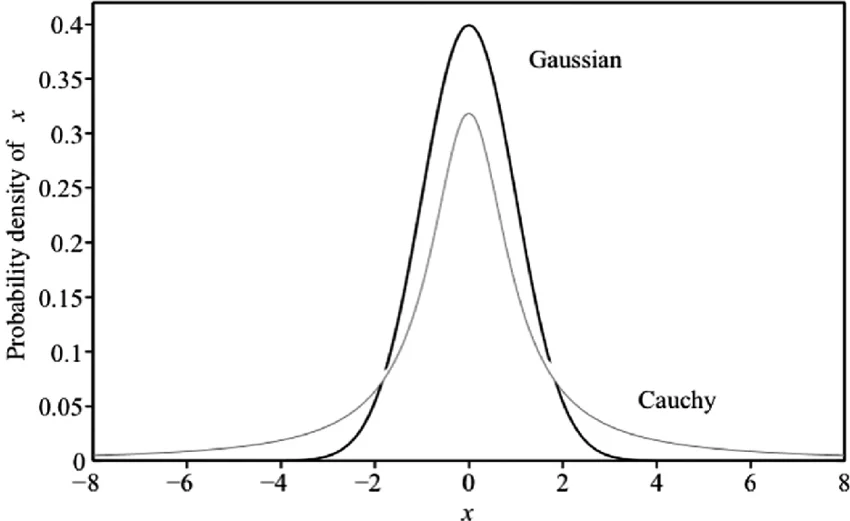
\includegraphics[width=0.5\linewidth]{gaussianvscauchy.png}
    \caption{Gaussian vs Cauchy distribution chart \parencite{cauchyvsgaussian}}
    \label{fig:cauchyvsgaussian}
\end{figure}
Figure \ref{fig:cauchyvsgaussian} shows the difference in the probability distribution of Gaussian and Cauchy distributions, showing that Cauchy distributions allow greater chances of greater variances. The modifications made for machine positions and angle were defined in Equation \ref{eq:cauchyx}, \ref{eq:cauchyy}, \ref{eq:cauchyrot}:
\begin{equation}
    x_i' = x_i + 2.0\,\delta_x, \qquad \delta_x \sim \mathrm{Cauchy}(0,1)
    \label{eq:cauchyx}
\end{equation}
\begin{equation}
    y_i' = y_i + 2.0\,\delta_y, \qquad \delta_y \sim \mathrm{Cauchy}(0,1)
    \label{eq:cauchyy}
\end{equation}
\begin{equation}
    \theta_i' = \theta_i + 20.0\,\delta_\theta, \qquad \delta_\theta \sim \mathrm{Cauchy}(0,1)
    \label{eq:cauchyrot}
\end{equation}
The Cauchy distribution of (0,1) means a location parameter $x_0 = 0$ and scale parameter of $\gamma=1$. These values are chosen for the distribution to be centered at 0 (fair positive and negative chances) and standard width through the $\gamma$ value. The Cauchy density function or probability density function through these values is shown in Equation \ref{eq:cauchyprobdensfunc},
\begin{equation}
    f(x)=\frac{1}{\pi(1+x^2)}
    \label{eq:cauchyprobdensfunc}
\end{equation}
Due to heavy tails in Cauchy distributions, large jumps occur more frequently as compared to Gaussian distributions. \textcite{gaussianandcauchypaper} proved that Cauchy distributions avoid local optima more efficiently than Gaussian distributions. In this paper, the modified rotation angle $\theta_i'$ was stored as is, until it would be snapped to the nearest 90$\circ$ at decoding during fitness evaluation, however this constraint can be removed or modified for other works of interest.

\item \textbf{Polynomial Mutation} \newline
Polynomial mutation was first introduced by \textcite{deb1996geneas} for genetic adaptive search for engineering designs, which was later described in more detail in \textcite{deb2001multiobjective} through evolutionary algorithms like GA. Polynomial mutation is a valid alternative for mutation strategies in GA as it enables the control of modification strength through the value of the distribution index $\eta$. Larger $\eta$ indicates smaller mutations, and vice versa for smaller $\eta$. Polynomial mutation modifies each gene according to Equation \ref{eq:polynomialmutationeq},
\begin{equation}
x_i' = x_i + \delta_i \cdot 0.1 \cdot (|x_i| + 1)
\label{eq:polynomialmutationeq}
\end{equation}
where
\[
\delta_i =
\begin{cases}
(2u)^{\frac{1}{\eta+1}} - 1, & u \le 0.5 \\[1ex]
1 - \bigl(2(1-u)\bigr)^{\frac{1}{\eta+1}}, & u > 0.5
\end{cases}
\]
with
\[
u \sim \mathcal{U}(0,1), \qquad \eta \text{ (distribution index)} = 20.
\]
Equation \ref{eq:polynomialmutationeq} applies to both $x$ and $y$ position mutations and also rotation angle $\theta$, where $\theta$ would be rounded to the nearest multiple of $90^\circ$. The values of $\eta$, and other variants of polynomial equations are modifiable according to the user's interest. These three different mutation strategies could be cycled by the RL agent by choosing action 7 (cycle mutation strategy). 
\end{itemize}
\subsection{Optimization Process}
The RL-GA optimization (see Figure \ref{fig:rlga_flowchart} proceeds iteratively as follows:
\begin{enumerate}
    \item Evaluate the current population fitness, then record the generation's best fitness, average fitness, and population diversity.
    \item Form the discrete RL state from population diversity and the improvement in fitness from the previous generation.
    \item Update Q-learning for all generations after the first by computing the reward from the change in best fitness since the last generation, and apply the Q-learning backup to the previous state--action pair using the new state as the successor state.
    \item Apply an action for the current state using an $\epsilon$-greedy policy, adjusting mutation rate, crossover rate, local search probability, mutation strategy, or performing a soft parameter reset. These settings govern the genetic operators in the remainder of this iteration.
    \item Run genetic algorithm process: preserve elites (with probabilistic local search applied to elites), then fill the remaining slots using tournament selection, crossover, and the active mutation operator.
    \item Replace the population with the new generation and update the tracked global best solution.
    \item Repeat steps 1-6 until the total number of generations is reached.
\end{enumerate}

Throughout each generations, the RL is designed to always perform an action that changes the parameters of the genetic algorithm, this means that the parameter settings of each generation will vary. The improvement and diversity are calculated for the previous generation before the generation when RL applies its actions. However, for the first generation case, since the initial improvement was set to $\infty$, it would always map to the significant improvement bin if there are any valid solutions within the initial population.
\begin{figure}[H]
\resizebox{\linewidth}{!}{%
\renewcommand{\baselinestretch}{1}\selectfont
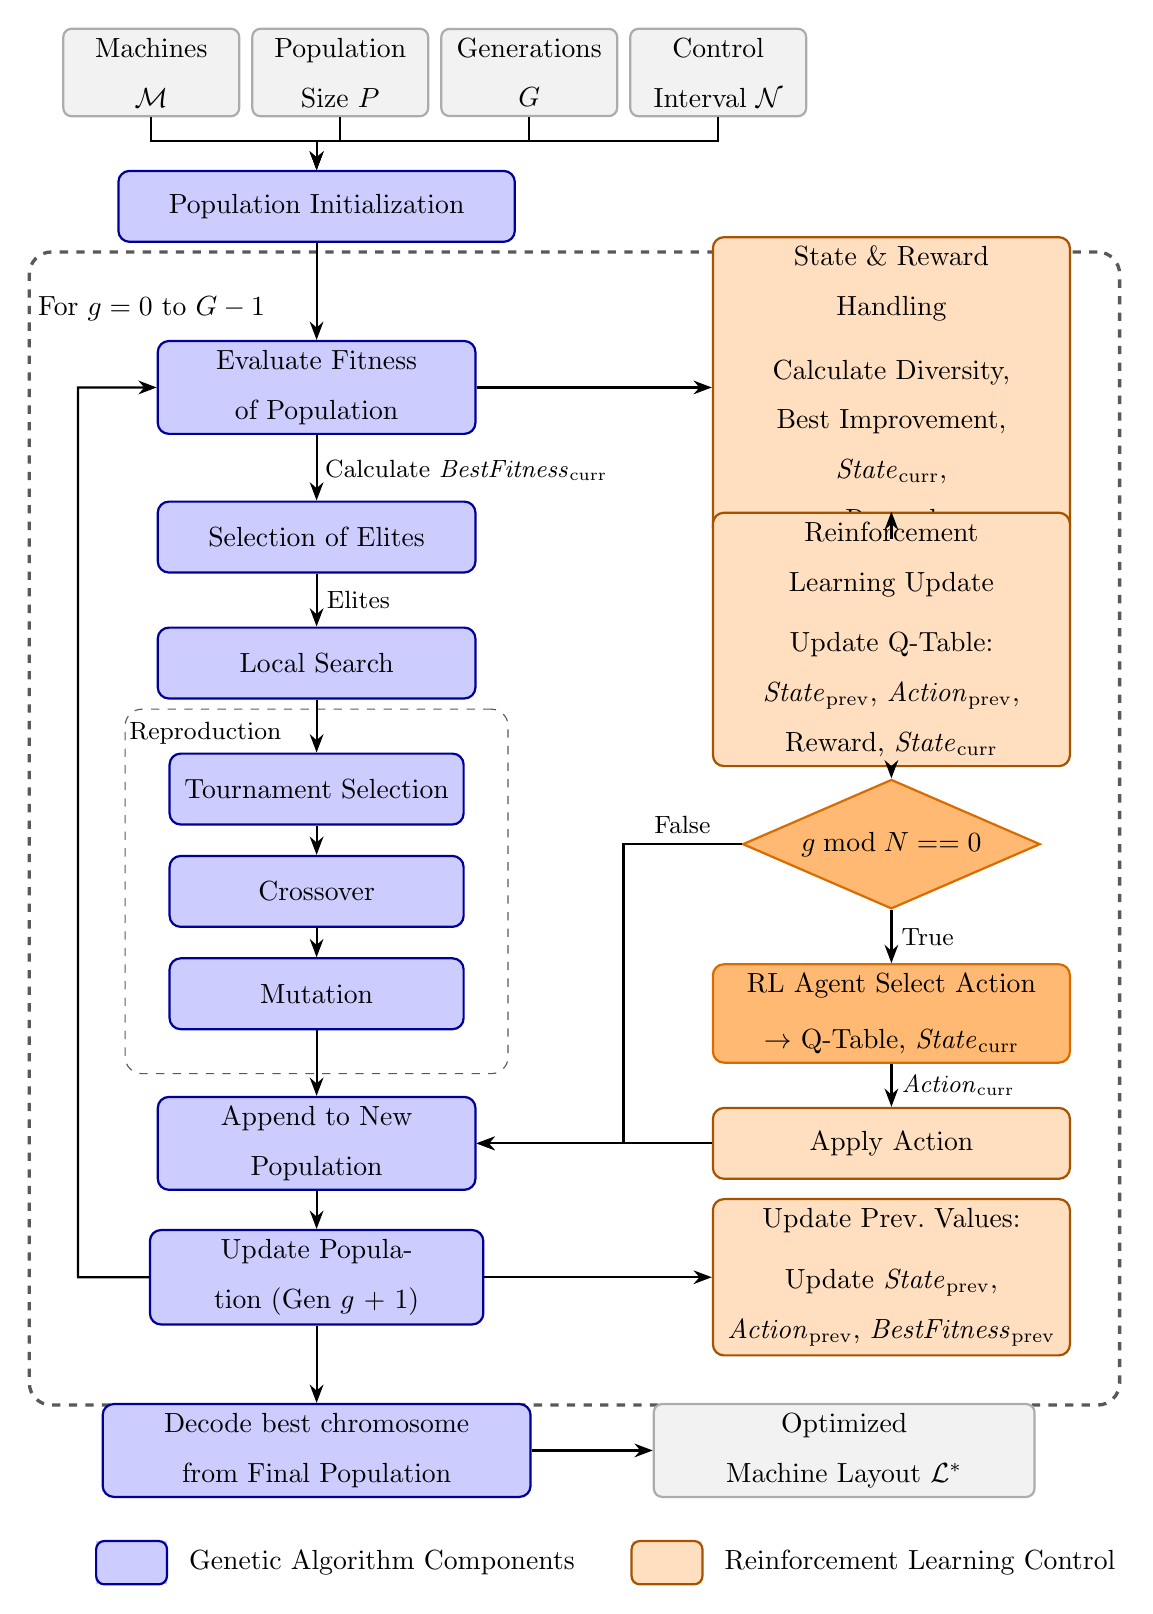
\begin{tikzpicture}[x=1cm, y=1cm, thick, >=Stealth,
  %-------- box styles --------
  gabox/.style={
    rectangle, rounded corners=4pt,
    draw=blue!60!black, fill=blue!20,
    minimum height=0.9cm, align=center
  },
  rlbox/.style={
    rectangle, rounded corners=4pt,
    draw=orange!65!black, fill=orange!25,
    align=center
  },
  rlboxd/.style={
    rectangle, rounded corners=4pt,
    draw=orange!85!black, fill=orange!55,
    minimum height=0.9cm, align=center
  },
  inpbox/.style={
    rectangle, rounded corners=3pt,
    draw=gray!65, fill=gray!10,
    minimum height=0.65cm, align=center
  },
  outbox/.style={
    rectangle, rounded corners=3pt,
    draw=gray!65, fill=gray!10,
    minimum height=0.65cm, align=center
  },
  diam/.style={
    diamond, draw=orange!85!black, fill=orange!55,
    aspect=2.3, minimum width=3.1cm, minimum height=0.9cm, align=center
  },
]

%%=============================================================
%% INPUTS ROW  (y = 22.5)
%%=============================================================
\node[inpbox, text width=2.0cm] (MACH)    at (1.9,  23) {Machines \\ $\mathcal{M}$};
\node[inpbox, text width=2.0cm] (POPSIZE) at (4.3,  23) {Population\\ Size $P$};
\node[inpbox, text width=2.0cm] (GENS)    at (6.7,  23) {Generations $G$};
\node[inpbox, text width=2.0cm] (CTRL)    at (9.1,  23) {Control\\ Interval $\mathcal{N}$};

%%=============================================================
%% POPULATION INITIALIZATION  (y = 20.8)
%%=============================================================
\node[gabox, text width=4.8cm] (POPINIT) at (4.0, 21.3)
  {Population Initialization};

\draw[->] (MACH.south)    -- ++(0,-0.3) -| (POPINIT.north);
\draw[->] (POPSIZE.south) -- ++(0,-0.3) -| (POPINIT.north);
\draw[->] (GENS.south)    -- ++(0,-0.3) -| (POPINIT.north);
\draw[->] (CTRL.south)    -- ++(0,-0.3) -| (POPINIT.north);

%%=============================================================
%% GA COLUMN  (centre x = 4.0)
%%=============================================================

%% Evaluate Fitness  (y = 19.0)
\node[gabox, text width=3.8cm] (EVALFIT) at (4.0, 19.0)
  {Evaluate Fitness\\ of Population};

% POPINIT → EVALFIT
\draw[->] (POPINIT.south) -- ++(0,-0.5) -| (EVALFIT.north);

% "Calculate BestFitness_curr" annotation (between EVALFIT and SELELITE)
\node[font=\small, align=center] at (5.9, 17.95)
  {Calculate $\mathit{BestFitness}_\mathrm{curr}$};

%% Selection of Elites  (y = 17.1)
\node[gabox, text width=3.8cm] (SELELITE) at (4.0, 17.1)
  {Selection of Elites};
\draw[->] (EVALFIT.south) -- (SELELITE.north);

%% Local Search  (y = 15.5)
\node[gabox, text width=3.8cm] (LOCSEARCH) at (4.0, 15.5)
  {Local Search};
\draw[->] (SELELITE.south) -- node[right, font=\small] {Elites} (LOCSEARCH.north);

%%--- Reproduction box: Tournament / Crossover / Mutation ---

\node[gabox, text width=3.5cm] (TOURNAMENT) at (4.0, 13.9)
  {Tournament Selection};
\node[gabox, text width=3.5cm] (CROSSOVER)  at (4.0, 12.6)
  {Crossover};
\node[gabox, text width=3.5cm] (MUTATION)   at (4.0, 11.3)
  {Mutation};

\draw[->] (LOCSEARCH.south) -- (TOURNAMENT.north);
\draw[->] (TOURNAMENT.south) -- (CROSSOVER.north);
\draw[->] (CROSSOVER.south)  -- (MUTATION.north);

% Loop arrow inside reproduction box: MUTATION right side → up → TOURNAMENT right side
% \draw[->] (MUTATION.east) -- ++(0.5, 0) |- (TOURNAMENT.east);

%% Dashed REPRODUCTION box
\begin{scope}[on background layer]
  \node[draw=black!65, dashed, rounded corners=6pt, inner sep=0.55cm,
        fit=(TOURNAMENT)(CROSSOVER)(MUTATION)] (REPBOX) {};
\end{scope}
\node[font=\small, anchor=north west, xshift=-2pt, yshift=-1pt]
  at (REPBOX.north west)
  {Reproduction};

%% Assemble NewPop  (y = 9.4)
\node[gabox, text width=3.8cm] (ASSEMBLENP) at (4.0, 9.4)
  {Append to New Population};
\draw[->] (MUTATION.south) -- ++(0,-0.65) -- (ASSEMBLENP.north);

%% Update Population  (y = 7.7)
\node[gabox, text width=4.0cm] (UPDATEPOP) at (4.0, 7.7)
  {Update Population (Gen $g+1$)};
\draw[->] (ASSEMBLENP.south) -- (UPDATEPOP.north);

%% Loop-back: UPDATEPOP.west → left → up → EVALFIT.west
\draw[->] (UPDATEPOP.west) -- ++(-0.9, 0)
  -- ++(0, 11.3)
  -- (EVALFIT.west);

% "Population (Gen g)" label to the left of the loop entry
% \node[font=\small, align=right, anchor=east]
%   at ($(EVALFIT.west)+(-0.3, 0.05)$)
%   {Population\\ (Gen $g$)};

%%=============================================================
%% RL COLUMN  (centre x = 11.3)
%%=============================================================

%% State & Reward Handling  (tall orange box, y = 17.7, height ≈ 3.4 cm)
\node[rlbox, text width=4.3cm, minimum height=2.5cm] (STATEREWARD) at (11.3, 19) {
  State \& Reward \\ Handling\\[5pt]
  Calculate Diversity,\\
  Best Improvement,\\
  $\mathit{State}_\mathrm{curr}$,\\
  Reward
};

\draw[->] (EVALFIT.east) -- ++(0.5, 0) |- (STATEREWARD.west);

%% Reinforcement Learning Update  (y = 14.6)
\node[rlbox, text width=4.3cm, minimum height=1.9cm] (RLUPDATE) at (11.3, 15.8) {
  Reinforcement Learning Update\\[4pt]
  Update Q-Table:\\
  $\mathit{State}_\mathrm{prev}$, $\mathit{Action}_\mathrm{prev}$,\\
  Reward, $\mathit{State}_\mathrm{curr}$
};
\draw[->] (STATEREWARD.south) -- (RLUPDATE.north);

%% Diamond: g mod N == 0  (y = 12.5)
\node[diam] (DIAMOND) at (11.3, 13.2) {$g \bmod N == 0$};
\draw[->] (RLUPDATE.south) -- (DIAMOND.north);
\draw[->] (DIAMOND.west) -- ++(-1.5,0) 
    node[midway, above, font=\small] {False}
    |- (ASSEMBLENP.east);

%% RL Agent Select Action – darker orange  (y = 10.9)
\node[rlboxd, text width=4.3cm, minimum height=1.1cm] (RLAGENT) at (11.3, 11.05) {
  RL Agent Select Action\\[2pt]
  $\to$ Q-Table, $\mathit{State}_\mathrm{curr}$
};
\draw[->] (DIAMOND.south) -- node[right, font=\small] {True} (RLAGENT.north);

%% Apply Action  (y = 9.4  — same as ASSEMBLENP for a clean horizontal arrow)
\node[rlbox, text width=4.3cm, minimum height=0.9cm] (APPLYACT) at (11.3, 9.4)
  {Apply Action};
\draw[->] (RLAGENT.south) --
  node[right, font=\small] {$\mathit{Action}_\mathrm{curr}$}
  (APPLYACT.north);

% Apply Action → Assemble NewPop (horizontal, same y level)
\draw[->] (APPLYACT.west) -- (ASSEMBLENP.east);

%% Update Prev. Values  (y = 7.7 — same as UPDATEPOP)
\node[rlbox, text width=4.3cm, minimum height=1.6cm] (UPDATEPREV) at (11.3, 7.7) {
  Update Prev.\ Values:\\[4pt]
  Update $\mathit{State}_\mathrm{prev}$,\\
  $\mathit{Action}_\mathrm{prev}$, $\mathit{BestFitness}_\mathrm{prev}$
};
% Update Population → Update Prev Values (horizontal, same y)
\draw[->] (UPDATEPOP.east) -- (UPDATEPREV.west |- UPDATEPOP.east);

%%=============================================================
%% MAIN LOOP DASHED BOX  ("FOR g = 0 to G − 1")
%%=============================================================
\begin{scope}[on background layer]

\coordinate (TOPLEFT)  at ($(EVALFIT.north west)+(-1.5,1)$);
\coordinate (BOTRIGHT) at ($(UPDATEPREV.south east)+(0.5,-0.5)$);

\node[
    draw=black!65,
    dashed,
    rounded corners=8pt,
    line width=1.2pt,
    fit=(TOPLEFT)(BOTRIGHT)
] (MAINLOOP) {};

\end{scope}

\node[
    font=\normalsize,
    anchor=north west,
    xshift=-0pt,
    yshift=-13pt
] at (MAINLOOP.north west)
{For $g = 0$ to $G - 1$};

%%=============================================================
%% OUTPUT (below loop)
%%=============================================================
\node[gabox, text width=5.2cm, minimum height=1.0cm] (DECODE) at (4.0, 5.5)
  {Decode best chromosome\\ from Final Population};
\draw[->] (UPDATEPOP.south) -- ++(0,-0.55) -| (DECODE.north);

\node[outbox, text width=4.6cm] (LSTAR) at (10.7, 5.5)
  {Optimized \\ Machine Layout $\mathcal{L}^*$};
\draw[->] (DECODE.east) -- (LSTAR.west);

%%=============================================================
%% LEGEND
%%=============================================================
\begin{scope}[shift={(1.2, 3.8)}]
  \fill[blue!20]  (0,0) rectangle (0.9, 0.55);
  \draw[blue!60!black, rounded corners=3pt] (0,0) rectangle (0.9, 0.55);
  \node[right, font=\normalsize] at (1.05, 0.275)
    {Genetic Algorithm Components};
\end{scope}
\begin{scope}[shift={(8.0, 3.8)}]
  \fill[orange!25] (0,0) rectangle (0.9, 0.55);
  \draw[orange!65!black, rounded corners=3pt] (0,0) rectangle (0.9, 0.55);
  \node[right, font=\normalsize] at (1.05, 0.275)
    {Reinforcement Learning Control};
\end{scope}

\end{tikzpicture}%
}
\caption{Flowchart of the optimization process of reinforcement learning genetic algorithm agent (RL-GA) for optimizing robotic workcells.}
\label{fig:rlga_flowchart}
\end{figure}

A key difference of RL-GA and standard GA optimization process is that during local search, RL-GA modifies the elites (top \% percentile of the population size), while standard GA applies local search to an offspring generated by the crossover, where the parents are randomly chosen to tournament selection. Hence, this study seeks to escape local minima or convergence through applying local search at elites, rather than offspring, which could balance exploration and exploitation, that would be explained at the Discussions section.

\subsection{Training}

Two tabular Q-learning agents were trained before being used for evaluation. RL-GA Agent 1 was trained on 8 layout problems using a GA configuration of population size 500 and 300 generations, while RL-GA Agent 2 was trained on 15 layout problems using a GA configuration of population size 200 and 300 generations. The training problems (1 to 15) are summarized in the Appendix.

For each agent, training was carried out over multiple epochs, where one epoch corresponds to one full pass over the entire training problem set. During each epoch, the same Q-learning agent was reused across all problems so that knowledge acquired from one layout instance could be transferred to subsequent instances. In each training run, the RL-assisted GA optimized a complete workcell layout while the agent continuously observed the current GA state, selected parameter-control actions, received rewards based on fitness improvement, and updated its Q-table.

The training problems were intentionally constructed to contain diverse machine geometries and access-point configurations, including rectangular and L-shaped machines of varying sizes, so that the learned policy would not overfit to a single layout pattern. All training problems used the same fixed processing sequence of eight machines, a robot starting position at the origin, and workspace bounds of $(-15,15,-15,15)$.

At the end of the training, the learned action-value table was saved as a NumPy array file. This stored Q-table was then reloaded during testing so that the trained RL agent could be deployed without retraining. During deployment, the exploration rate $\epsilon$ can be reduced to zero so that the trained policy acts greedily according to the learned Q-values.

In summary, the training process consists of the following steps:
\begin{enumerate}
    \item Define a set of training layout problems.
    \item Initialize a shared Q-learning agent with discrete state and action spaces.
    \item Run RL-GA on each training problem for several epochs.
    \item Update the Q-table online from generation-to-generation rewards.
    \item Save the final Q-table for later testing and reuse.
\end{enumerate}

\newpage
\section{Results: Standard Genetic Algorithm}
\subsection{Sample Problem}
This robotic workcell example consists of eight machines with mixed geometries, including both rectangular and L-shaped configurations. Each machine is defined by its dimensions, and access point location. The machine geometries used in this experiment are given in Table \ref{tab:machine_config}:

\begin{table}[H]
\centering
\begin{tabular}{ccccccc}
\toprule
\textbf{ID} & \textbf{Shape} & \textbf{Width} & \textbf{Height} & \textbf{Access Point (x, y)} & \textbf{Cutout Width} & \textbf{Cutout Height} \\
\midrule
M1 & L-shape   & 5.21 & 4.33 & (1.48, -1.12) & 2.01 & 1.72 \\
M2 & Rectangle & 4.87 & 3.12 & (0.92, -0.44) & --   & --   \\
M3 & L-shape   & 4.56 & 5.46 & (-0.72, 1.89) & 1.58 & 2.74 \\
M4 & Rectangle & 3.44 & 2.61 & (0.13, 0.89)  & --   & --   \\
M5 & L-shape   & 5.94 & 3.77 & (1.04, -0.88) & 2.23 & 1.32 \\
M6 & Rectangle & 4.32 & 2.48 & (-0.63, -0.41) & --  & --   \\
M7 & L-shape   & 3.88 & 4.91 & (0.55, 1.22)  & 1.25 & 2.01 \\
M8 & Rectangle & 3.27 & 2.74 & (0.15, -0.52) & --   & --   \\
\bottomrule
\end{tabular}
\caption{Machine Configuration for the Sample Problem}
\label{tab:machine_config}
\end{table}
\vspace{-20pt}
The sequence are given in increasing order of Machine 1 to Machine 8, with workspace boundaries set as (-15, 15, -15, 15). Figure \ref{fig:sample problem ga comparison} shows the layout results obtained from standard Genetic Algorithm optimization for initial population generation and final optimized layout. The number of population is set to 200, and number of generations to 300 (according to default value in Table \ref{tab:ga_parameters}).

\begin{figure}[H]
    \centering
    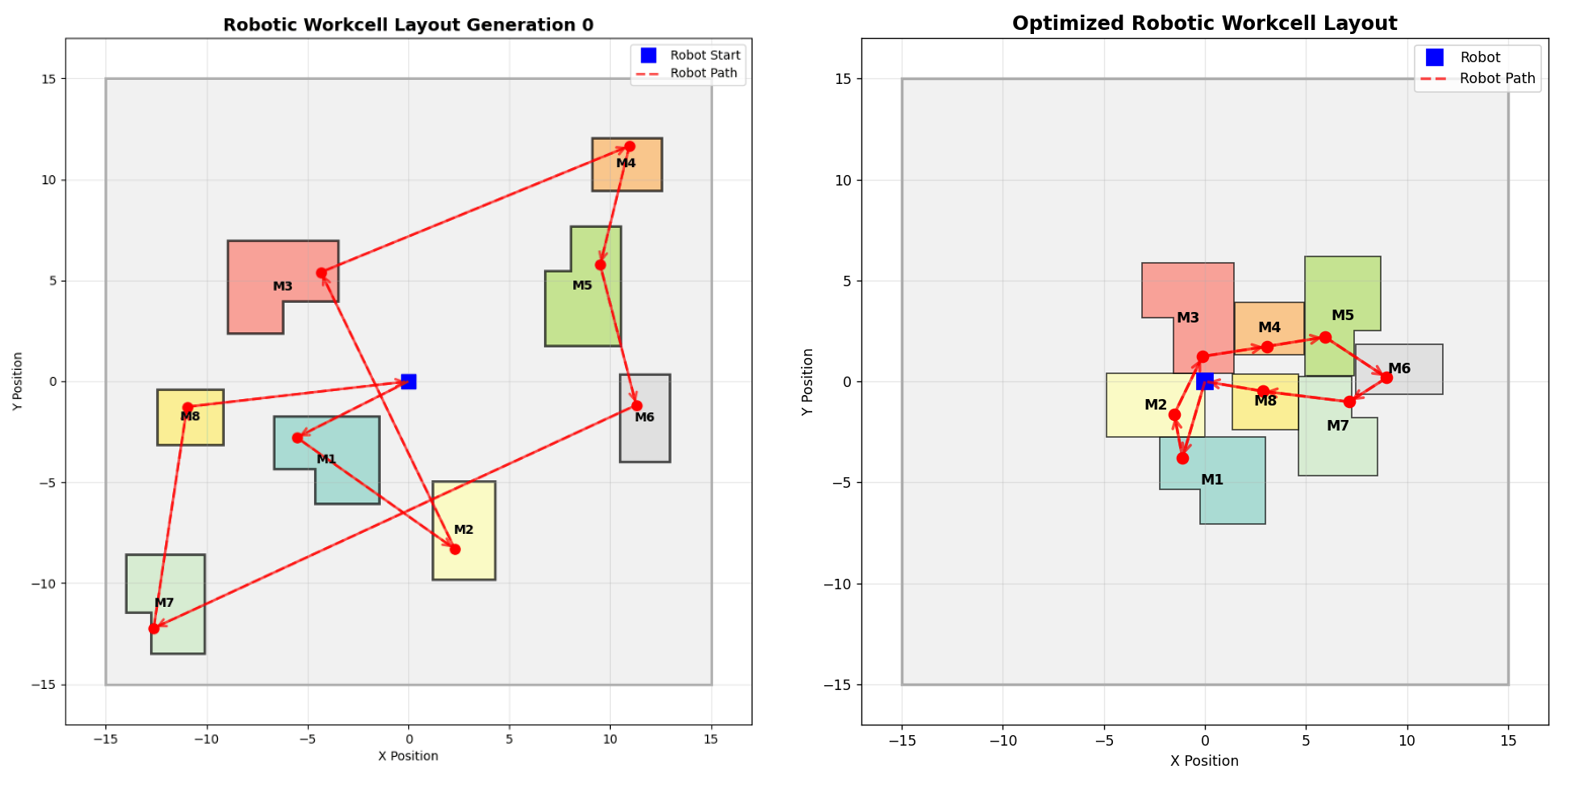
\includegraphics[width=0.9\linewidth]{results_pure_ga_evolution/comparison.png}
    \caption{Layout comparison for initial population (generation 0) and final population (generation 300)}
    \label{fig:sample problem ga comparison}
\end{figure}

\begin{table}[H]
\centering
\begin{tabular}{ccc}
\toprule
\textbf{Generation} & \textbf{Best Fitness} & \textbf{Average Fitness} \\
\midrule
0   & 111.77 & 138.85 \\
20  & 61.98  & 71.67  \\
40  & 42.17  & 48.46  \\
60  & 36.15  & 39.23  \\
80  & 33.56  & 36.04  \\
100 & 32.46  & 35.21  \\
120 & 31.60  & 33.21  \\
140 & 31.15  & 33.27  \\
160 & 30.92  & 32.30  \\
180 & 30.64  & 32.81  \\
200 & 30.14  & 32.77  \\
220 & 30.12  & 31.91  \\
240 & 30.08  & 31.55  \\
260 & 30.07  & 30.99  \\
280 & 30.06  & 31.11  \\
300 & 30.01  & 30.93  \\
\bottomrule
\end{tabular}
\caption{Genetic Algorithm Optimization Progress}
\label{tab:ga_progress}
\end{table}
Table \ref{tab:ga_progress} shows the evolution of the best and average fitness from generations 0 (initial population) to generations 300 (final optimized layout). The execution time was recorded as 221.71 seconds. Finally, the total distance needed for the robot to travel is calculated as 28.54 units.

In the next sections, for each population size and number of generations, the initial populations and hyperparameters of the genetic algorithm are kept the same to ensure fairness of comparison. The same sample problem machine configurations in Table \ref{tab:machine_config} are also used for the population and generation for the next standard GA experiments.

\subsection{Various Populations and Generation Sizes}
\begin{table}[H]
\centering
\begin{tabular}{cccccc}
\toprule
\textbf{Population} & \textbf{Generations} & \textbf{Final Best Fitness} & \textbf{Final Avg Fitness} & \textbf{Final Diversity} & \textbf{Execution Time (s)} \\
\midrule
100 & 100 & 41.54 & 44.19 & 182.23 & 30.69 \\
 & 200 & 36.66 & 38.09 & 142.36 & 63.63 \\
 & 500 & 36.49 & 38.76 & 155.98 & 160.48 \\
 & 1000 & 36.35 & 37.03 & 135.83 & 322.73 \\
 & 2000 & 36.34 & 36.84 & 132.13 & 648.30 \\
\midrule
200 & 100 & 40.25 & 42.30 & 210.79 & 63.21 \\
 & 200 & 35.79 & 37.10 & 165.83 & 129.67 \\
 & 500 & 35.64 & 36.81 & 195.79 & 331.45 \\
 & 1000 & 32.15 & 33.38 & 184.92 & 666.13 \\
 & 2000 & 32.09 & 33.49 & 164.08 & 1352.28 \\
\midrule
500 & 100 & 37.44 & 39.52 & 158.44 & 176.66 \\
 & 200 & 36.15 & 37.82 & 152.99 & 368.36 \\
 & 500 & 33.90 & 35.49 & 143.11 & 943.46 \\
 & 1000 & 33.53 & 35.25 & 151.34 & 1919.62 \\
 & 2000 & 33.46 & 34.90 & 137.61 & 3874.17 \\
\midrule
1000 & 100 & 41.65 & 45.13 & 185.32 & 386.98 \\
 & 200 & 38.78 & 39.83 & 162.17 & 833.22 \\
 & 500 & 37.00 & 38.32 & 164.89 & 2170.48 \\
 & 1000 & 36.84 & 37.80 & 161.34 & 4423.15 \\
 & 2000 & 36.80 & 38.18 & 172.93 & 8939.52 \\
\midrule
2000 & 100 & 37.84 & 40.31 & 167.54 & 1212.15 \\
 & 200 & 36.69 & 38.56 & 159.69 & 2487.17 \\
 & 500 & 36.50 & 37.91 & 154.65 & 6280.36 \\
 & 1000 & 36.21 & 37.77 & 167.65 & 12636.03 \\
 & 2000 & 35.94 & 37.45 & 168.81 & 25364.26 \\
\bottomrule
\end{tabular}
\caption{Summary of standard GA results across population size and generation count}
\label{tab:ga_grid_summary}
\end{table}
Table \ref{tab:ga_grid_summary} summarizes the final metrics for generations up to 100, 200, 500, and 1000. The comparison figures are placed in the Appendix for further reference and visualization. A consistent trend can be observed where larger number in generations would guarantee better fitness (lower fitness in this task), but with a trade-off of approximately more than double the increase in execution time when the number of generations are doubled (e.g., for population 100: 30.69 s to 63.63 s $\approx$ +107.33\%, and 160.48 s to 322.73 s $\approx$ +101.10\%). On the other hand, increasing in number of population did not guarantee better fitness, but similar to number of populations, it took approximately twice to thrice more execution time (200 – 310\%) for twice of the population size, especially for larger population sizes (e.g., at 100 generations: 30.69 s to 63.21 s $\approx$ +106\%, and 386.98 s to 1212.15 s $\approx$ +213\%).

In terms of fitness improvement, major improvements are recorded from generations 100 to 200, where the average improvement is approximately 7.24\%, computed from individual relative improvements of about 11.75\% (pop 100), 11.08\% (pop 200), 3.45\% (pop 500), 6.89\% (pop 1000), and 3.04\% (pop 2000). For later generations, particularly 500 to 1000, the average improvements were recorded to be approximately 2.50\%, however, population size of 200 displays a rather big improvement compared to the rest at about 9.88\% improvement. For generations from 1000 to 2000, the improvements become more negligible, with an average improvement of approximately 0.26\%.

The diversity was observed to decrease in increasing number of generations as a general trend. Regarding the rate of decrease, diversity decreases rapidly at earlier generations (generations 0 to 100), with particular patterns at generations 20 to 40 (see Appendix). At earlier generations, the diversity values were calculated to be approximately around 300 to 400, where at later generations it shrank down to the 100s as shown in Table \ref{tab:ga_grid_summary}. During this experiment, there were also fluctuations in diversity observed due to the stochastic nature of genetic operations, typically indicating a spike in diversity as more solutions explored at that particular generation. 

These results are discussed in the Discussion section (Chapter 11), where the numerical values would be meaningfully interpreted and analyzed for the standard GA behavior, and also as a means to design the RL-GA agent state-reward configurations.


\newpage
\section{Results: GA vs RL-GA Agent 1}
In this results section, RL-GA Agent 1 is trained through 8 different problems with population size of 500, and generation number of 300. 
The testing compares Genetic Algorithm (GA) against Reinforcement-Learning-GA (RL-GA) across 10 benchmark problems using the metrics reported in the experiment log: average fitness, best fitness, average total distance, and execution time. The number of runs for the 10 problems was set to 3. The 10 problems' machine geometries and properties were summarized in the Appendix.

\subsection{Sample Problem}
The same problem as stated in Section 8.1 was used again for this sample problem comparison for standard GA and RL-GA Agent 1 sample experiment. The number of populations for standard GA and RL-GA was set to 200, although RL-GA was trained with a population size of 500. This setup was designed to fairly assess both agents (RL-GA Agents 1 and 2) with the same initial population, and assumes that the learned policy generalizes across different population sizes, which is reasonable because the state representation is based on normalized diversity and improvement metrics rather than absolute population characteristics.

\subsubsection{RL-GA Parameter Control}
\begin{figure}[H]
    \centering
    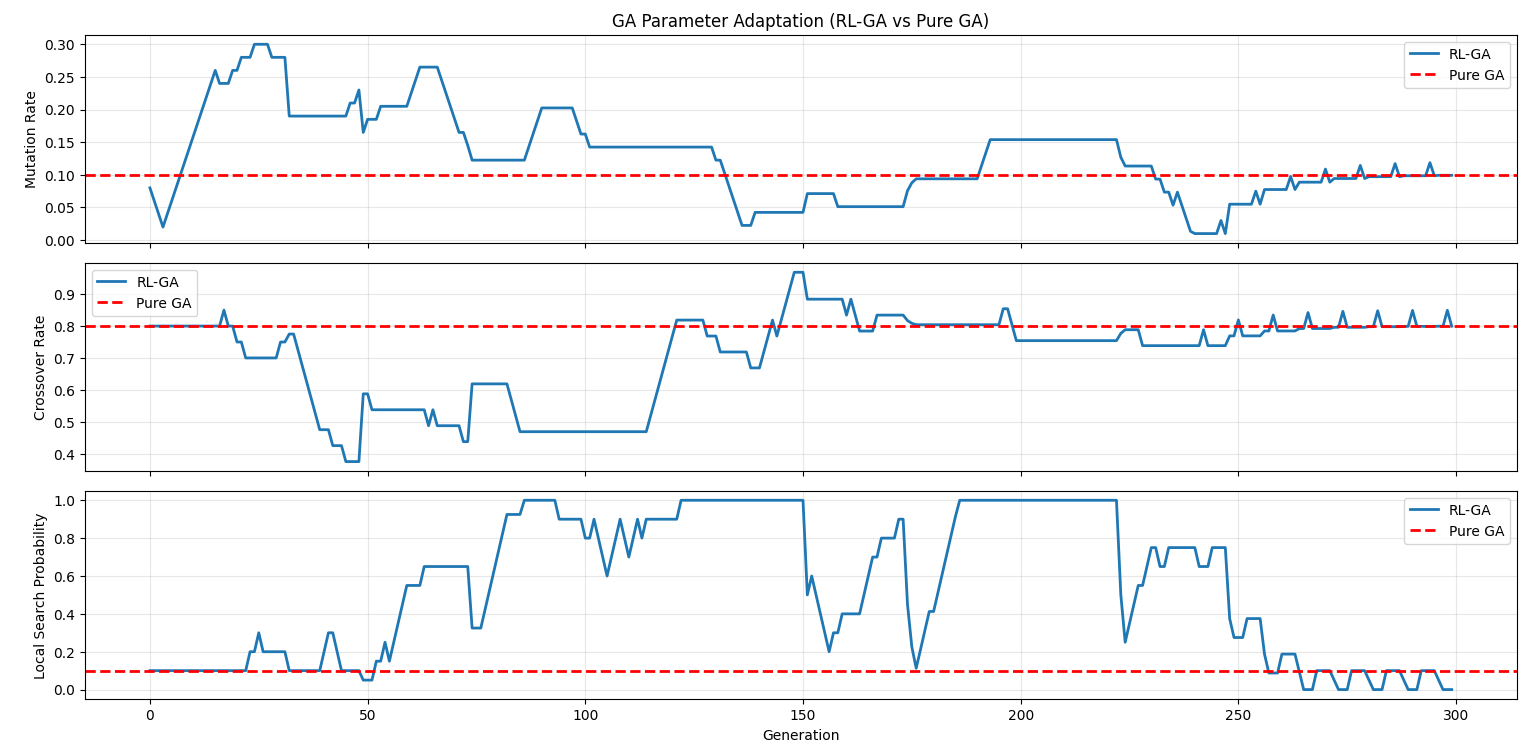
\includegraphics[width=0.95\linewidth]{pure_ga_vs_agent_1_sample/parametergraph.png}
    \caption{GA parameter values due to RL agent adaptive actions against the number of generations}
    \label{fig:sample_rl_vs_ga_parameters}
\end{figure}
\vspace{-20pt}
Figure \ref{fig:sample_rl_vs_ga_parameters} shows the GA parameter values through the dynamic control of RL-GA Agent 1, compared to the static standard GA settings. The mutation rate spiked at earlier generations (around 0 to 30), where it reached its peak of 0.3 at generation 24. It then flattened and gradually decreased for later generations, eventually reaching a minimum value of 0.010 around generation 240. The crossover rate shows a rather sinusoidal behavior throughout the generations, where its lowest value was recorded as 0.375 at generation 45. Lastly, the local search probability began to escalate rapidly from generations 50 and above, where it even reached a 1.0 value at generation 86 for a the later ranges of generations. However, it decreased for later generations which were reaching 300.
\subsubsection{Optimized Layout Comparison}
\begin{figure}[H]
    \centering
    \begin{subfigure}{0.48\linewidth}
        \centering
        
\includegraphics[width=\linewidth]{pure_ga_vs_agent_1_sample/rl_optimized_layout.png}
        \caption{RL-GA Agent 1 optimized layout}
    \end{subfigure}
    \hfill
    \begin{subfigure}{0.48\linewidth}
        \centering
        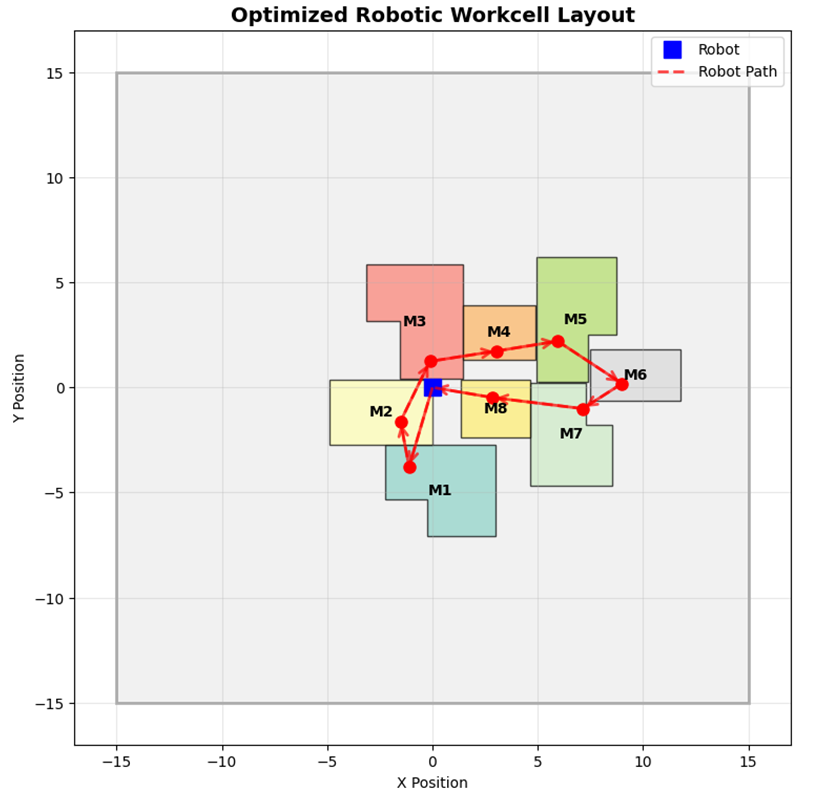
\includegraphics[width=\linewidth]{pure_ga_vs_agent_1_sample/ga_optimized_layout.png}
        \caption{Standard GA optimized layout}
    \end{subfigure}
    
    \caption{Comparison of optimization performance and resulting layouts for the sample problem}
    \label{fig:rl_ga_comparison}
\end{figure}
\begin{table}[H]
\centering
\small
\setlength{\tabcolsep}{6pt}
\renewcommand{\arraystretch}{1.2}
\begin{tabular}{c c c c c c c}
\toprule
\multirow{2}{*}{\textbf{Machine}} 
& \multicolumn{3}{c}{\textbf{Standard GA}} 
& \multicolumn{3}{c}{\textbf{RL-GA Agent 1}} \\
\cmidrule(lr){2-4} \cmidrule(lr){5-7}
& \textbf{X} & \textbf{Y} & \textbf{Rot ($^\circ$)} 
& \textbf{X} & \textbf{Y} & \textbf{Rot ($^\circ$)} \\
\midrule
1 & 0.37  & -4.90 & 180 & -1.93 & -3.57 & 90 \\
2 & -2.44 & -1.17 & 0   & -2.44 & 0.60  & 0 \\
3 & -0.84 & 3.13  & 180 & -0.10 & 4.90  & 180 \\
4 & 3.19  & 2.62  & 180 & 3.49  & 3.61  & 270 \\
5 & 6.82  & 3.24  & 270 & 6.68  & 4.01  & 270 \\
6 & 9.63  & 0.59  & 0   & 5.98  & -0.20 & 0 \\
7 & 6.59  & -2.23 & 0   & 3.12  & -3.32 & 0 \\
8 & 3.01  & -1.00 & 180 & 1.64  & 0.51  & 0 \\
\bottomrule
\end{tabular}
\caption{Comparison of machine configurations between Standard GA (Fitness = 30.01) and RL-GA Agent 1 (Fitness = 25.13)}
\label{tab:ga_vs_rlga_layout}
\end{table}
\vspace{-20pt}
Figure \ref{fig:rl_ga_comparison} shows the finalized layout from the standard GA and RL-GA Agent 1 computation for 300 generations. The standard GA achieves the best fitness of 30.01, while the RL-GA Agent 1 achieves the best fitness of 25.13, which is 16.26\% better than standard GA. Table \ref{tab:ga_vs_rlga_layout} summarizes the machines' global locations and final rotations that correspond to Figure \ref{fig:rl_ga_comparison}.
\subsubsection{Fitness Convergence}
\begin{figure}[H]
    \centering
    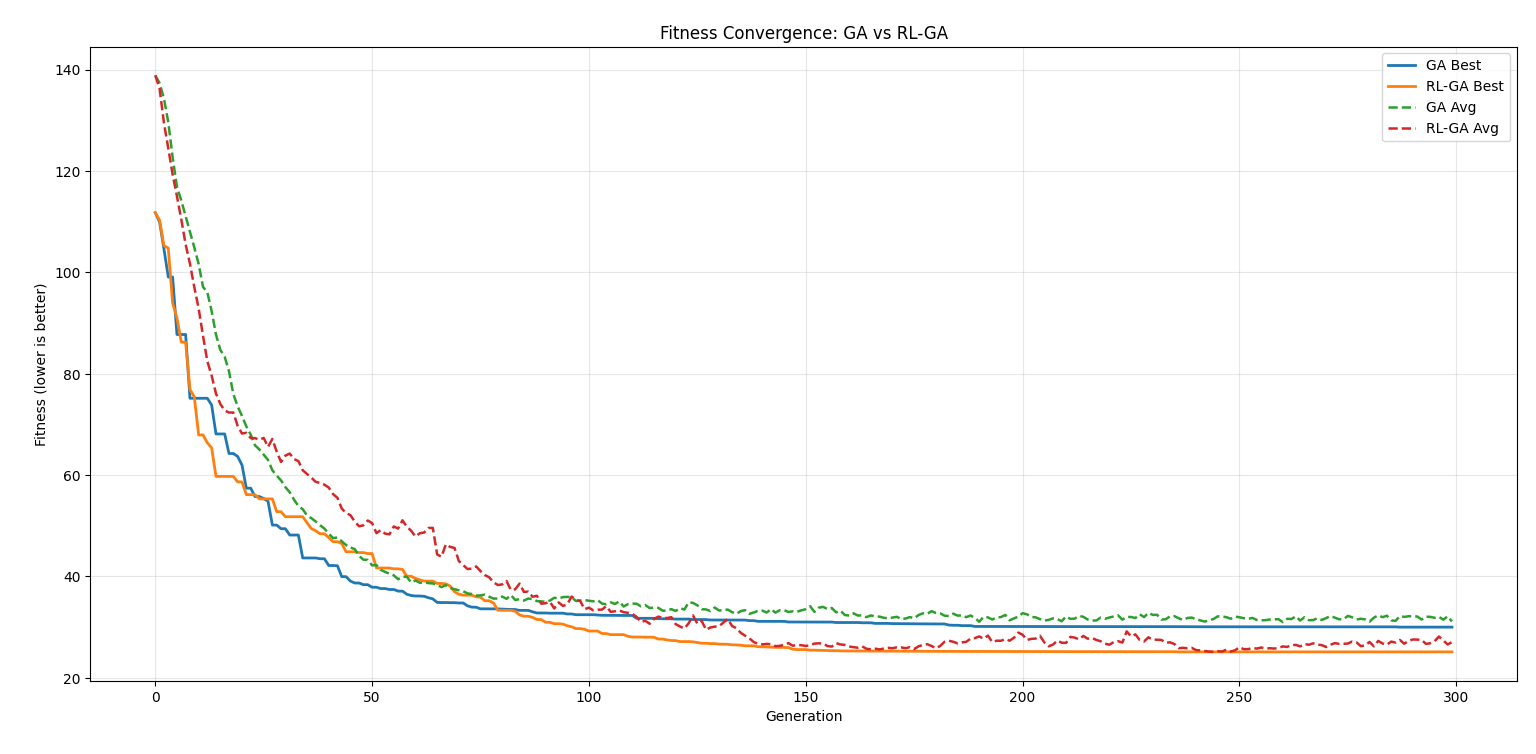
\includegraphics[width=0.8\linewidth]{pure_ga_vs_agent_1_sample/fitness_convergence.png}
    \caption{Fitness convergence graph comparison of sample problem for standard GA and RL-GA Agent 1}
    \label{fig:placeholder}
\end{figure}
\begin{table}[H]
\centering
\begin{tabular}{ccccccc}
\toprule
\textbf{Generation} & \textbf{Algorithm} & \textbf{Best Fitness} & \textbf{Average Fitness} & \textbf{Diversity} \\
\midrule
0   & Standard GA & 111.77 & 138.85 & 416.098 \\
0   & RL-GA   & 111.77 & 138.85 & 416.098 \\
\midrule
60  & Standard GA & 36.15  & 39.23  & 208.382 \\
60  & RL-GA   & 39.63  & 47.89  & 327.90 \\
\midrule
120 & Standard GA & 31.60  & 33.21  & 165.909 \\
120 & RL-GA   & 27.34  & 30.60  & 266.59 \\
\midrule
180 & Standard GA & 30.64  & 32.81  & 176.715 \\
180 & RL-GA   & 25.22  & 25.85  & 147.53 \\
\midrule
240 & Standard GA & 30.08  & 31.55  & 161.184 \\
240 & RL-GA   & 25.13  & 25.48  & 44.44 \\
\midrule
300 & Standard GA & 30.01  & 30.93  & 134.044 \\
300 & RL-GA   & 25.13  & 25.48  & 150.00 \\
\bottomrule
\end{tabular}
\caption{Fitness and diversity comparison between standard GA and RL-GA at selected generations}
\label{tab:ga_rlga_1_sample_problem}
\end{table}
\vspace{-25pt}
Table \ref{tab:ga_rlga_1_sample_problem} shows the fitness evolution for increments of 60 generations. At earlier generations, RL-GA Agent 1 converged slower than the standard GA, where the diversity is also shown to be more than the standard GA. However, at approximately generations 100 onward, RL-GA Agent 1 escaped local optima much faster than standard GA until approximately generations 150, where both started to subside until the end. For the execution time, GA reached 300 completed at 218.41 seconds while RL-GA Agent 1 at 238.59 seconds (9.24\% longer).
\subsection{Experiment with 10 Problems}
\subsubsection{Figures}
\begin{figure}[H]
    \centering
    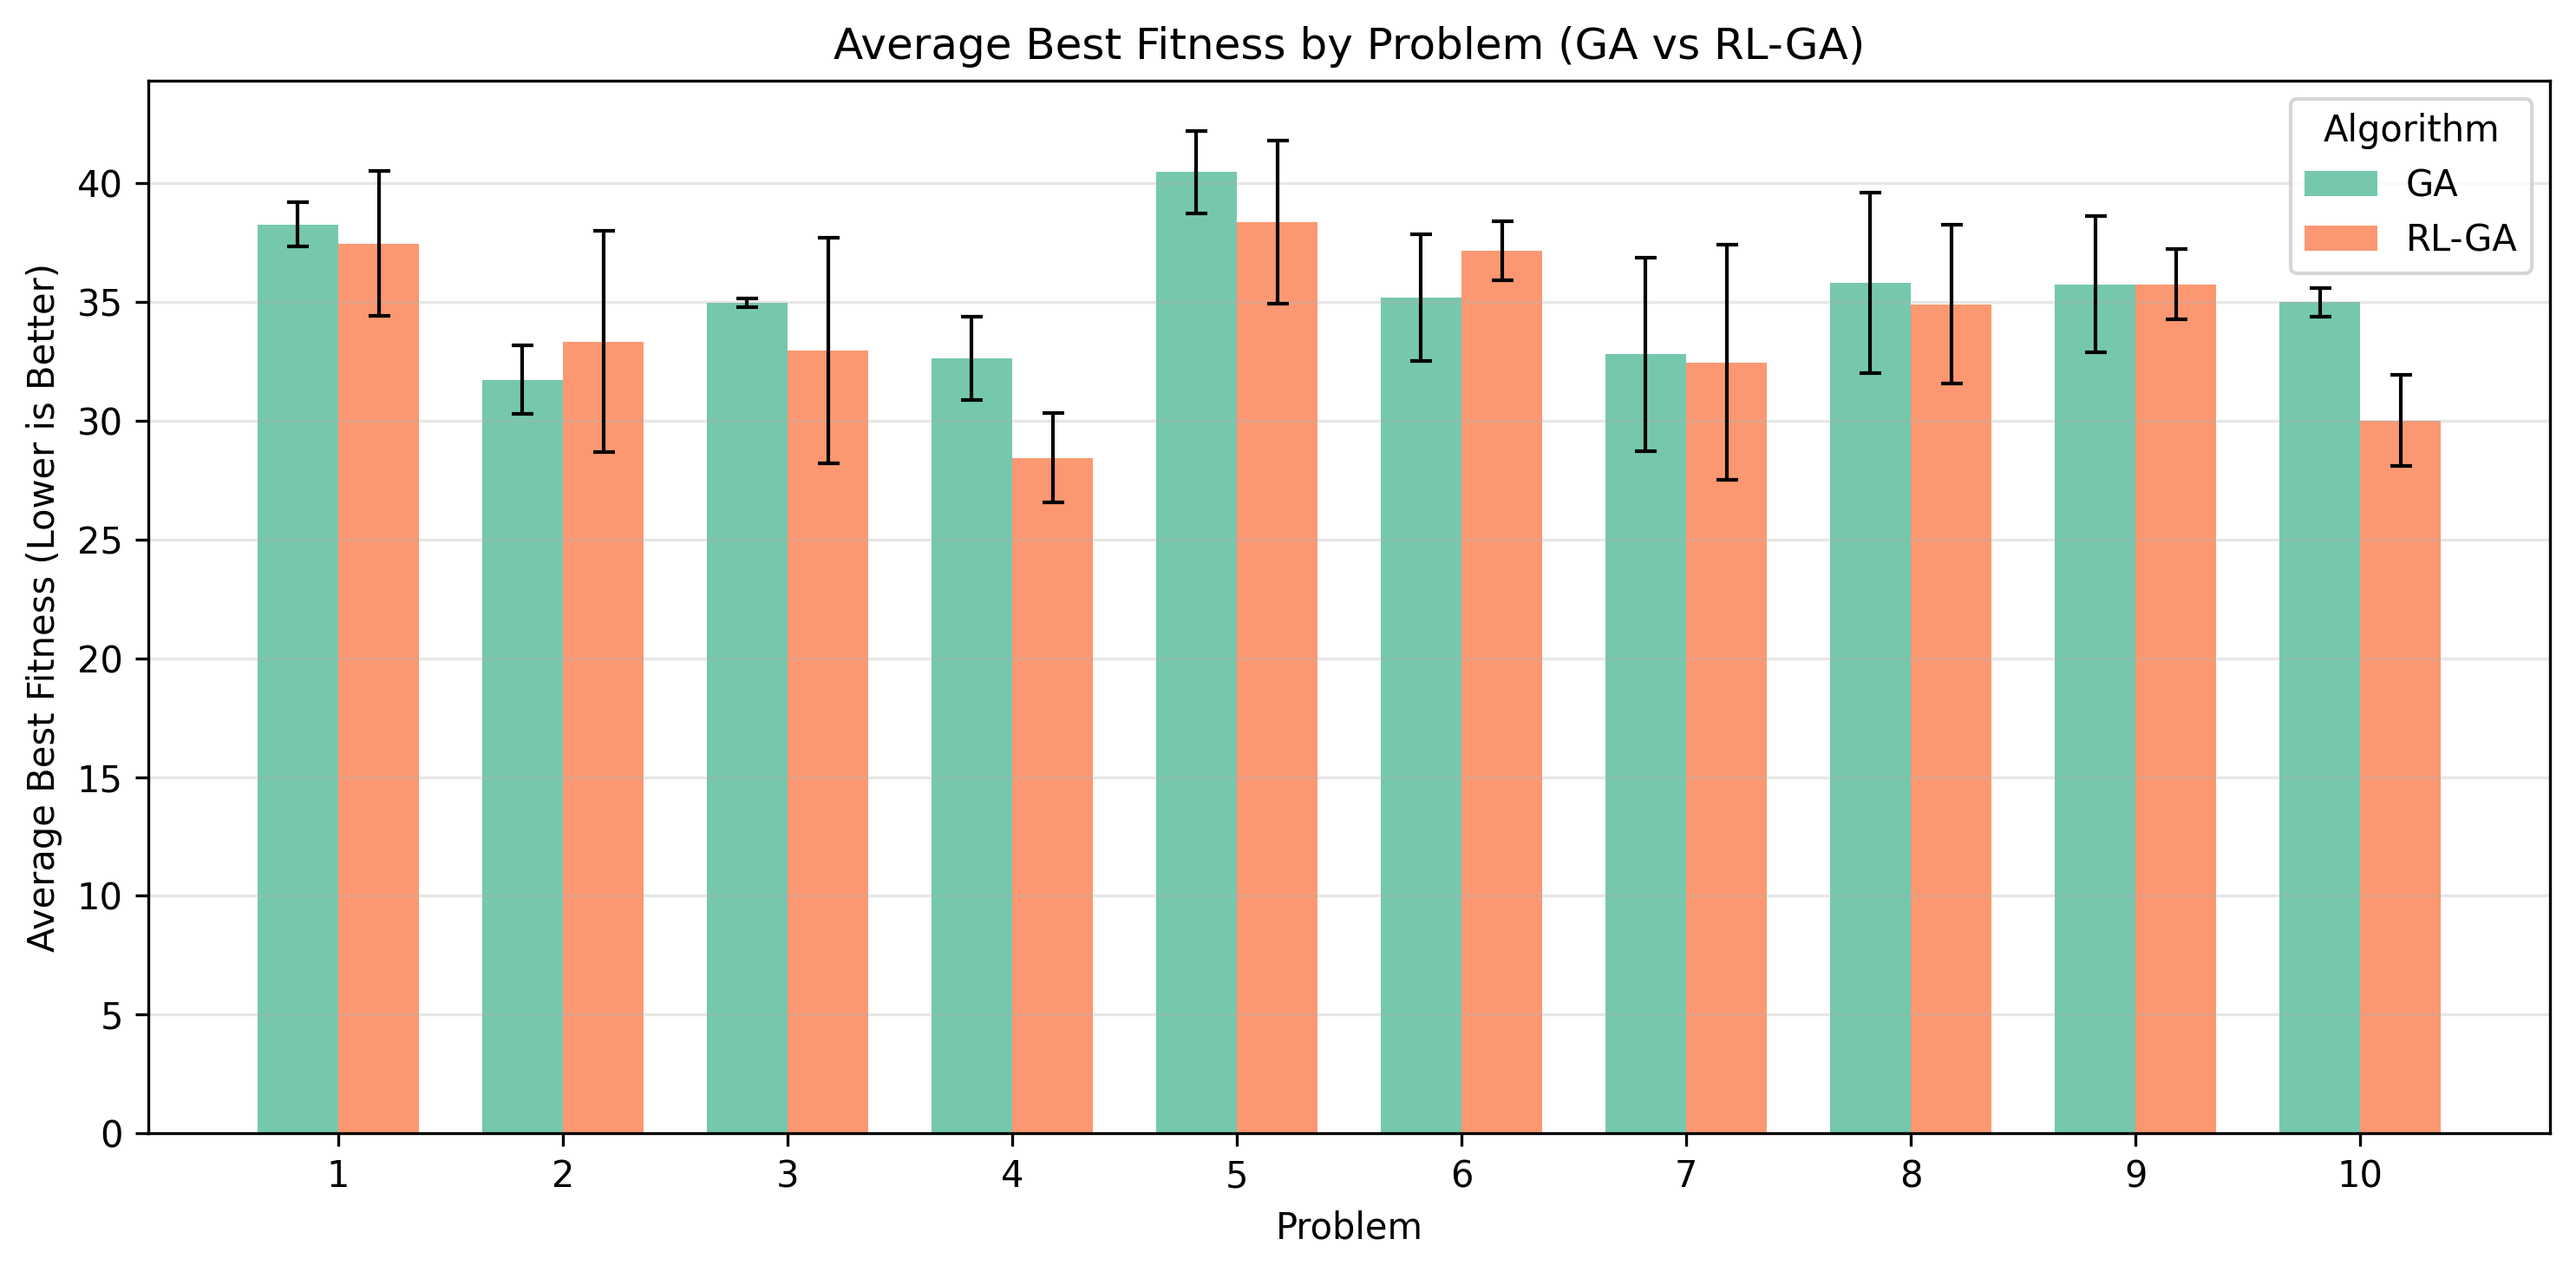
\includegraphics[width=0.67\linewidth]{results_500_300_8/best_fitness_avg.png}
    \caption{Bar plot of average best fitness for 10 random problems for standard GA and RL-GA Agent 1}
    \label{fig:placeholder}
\end{figure}
\begin{figure}[H]
    \centering
    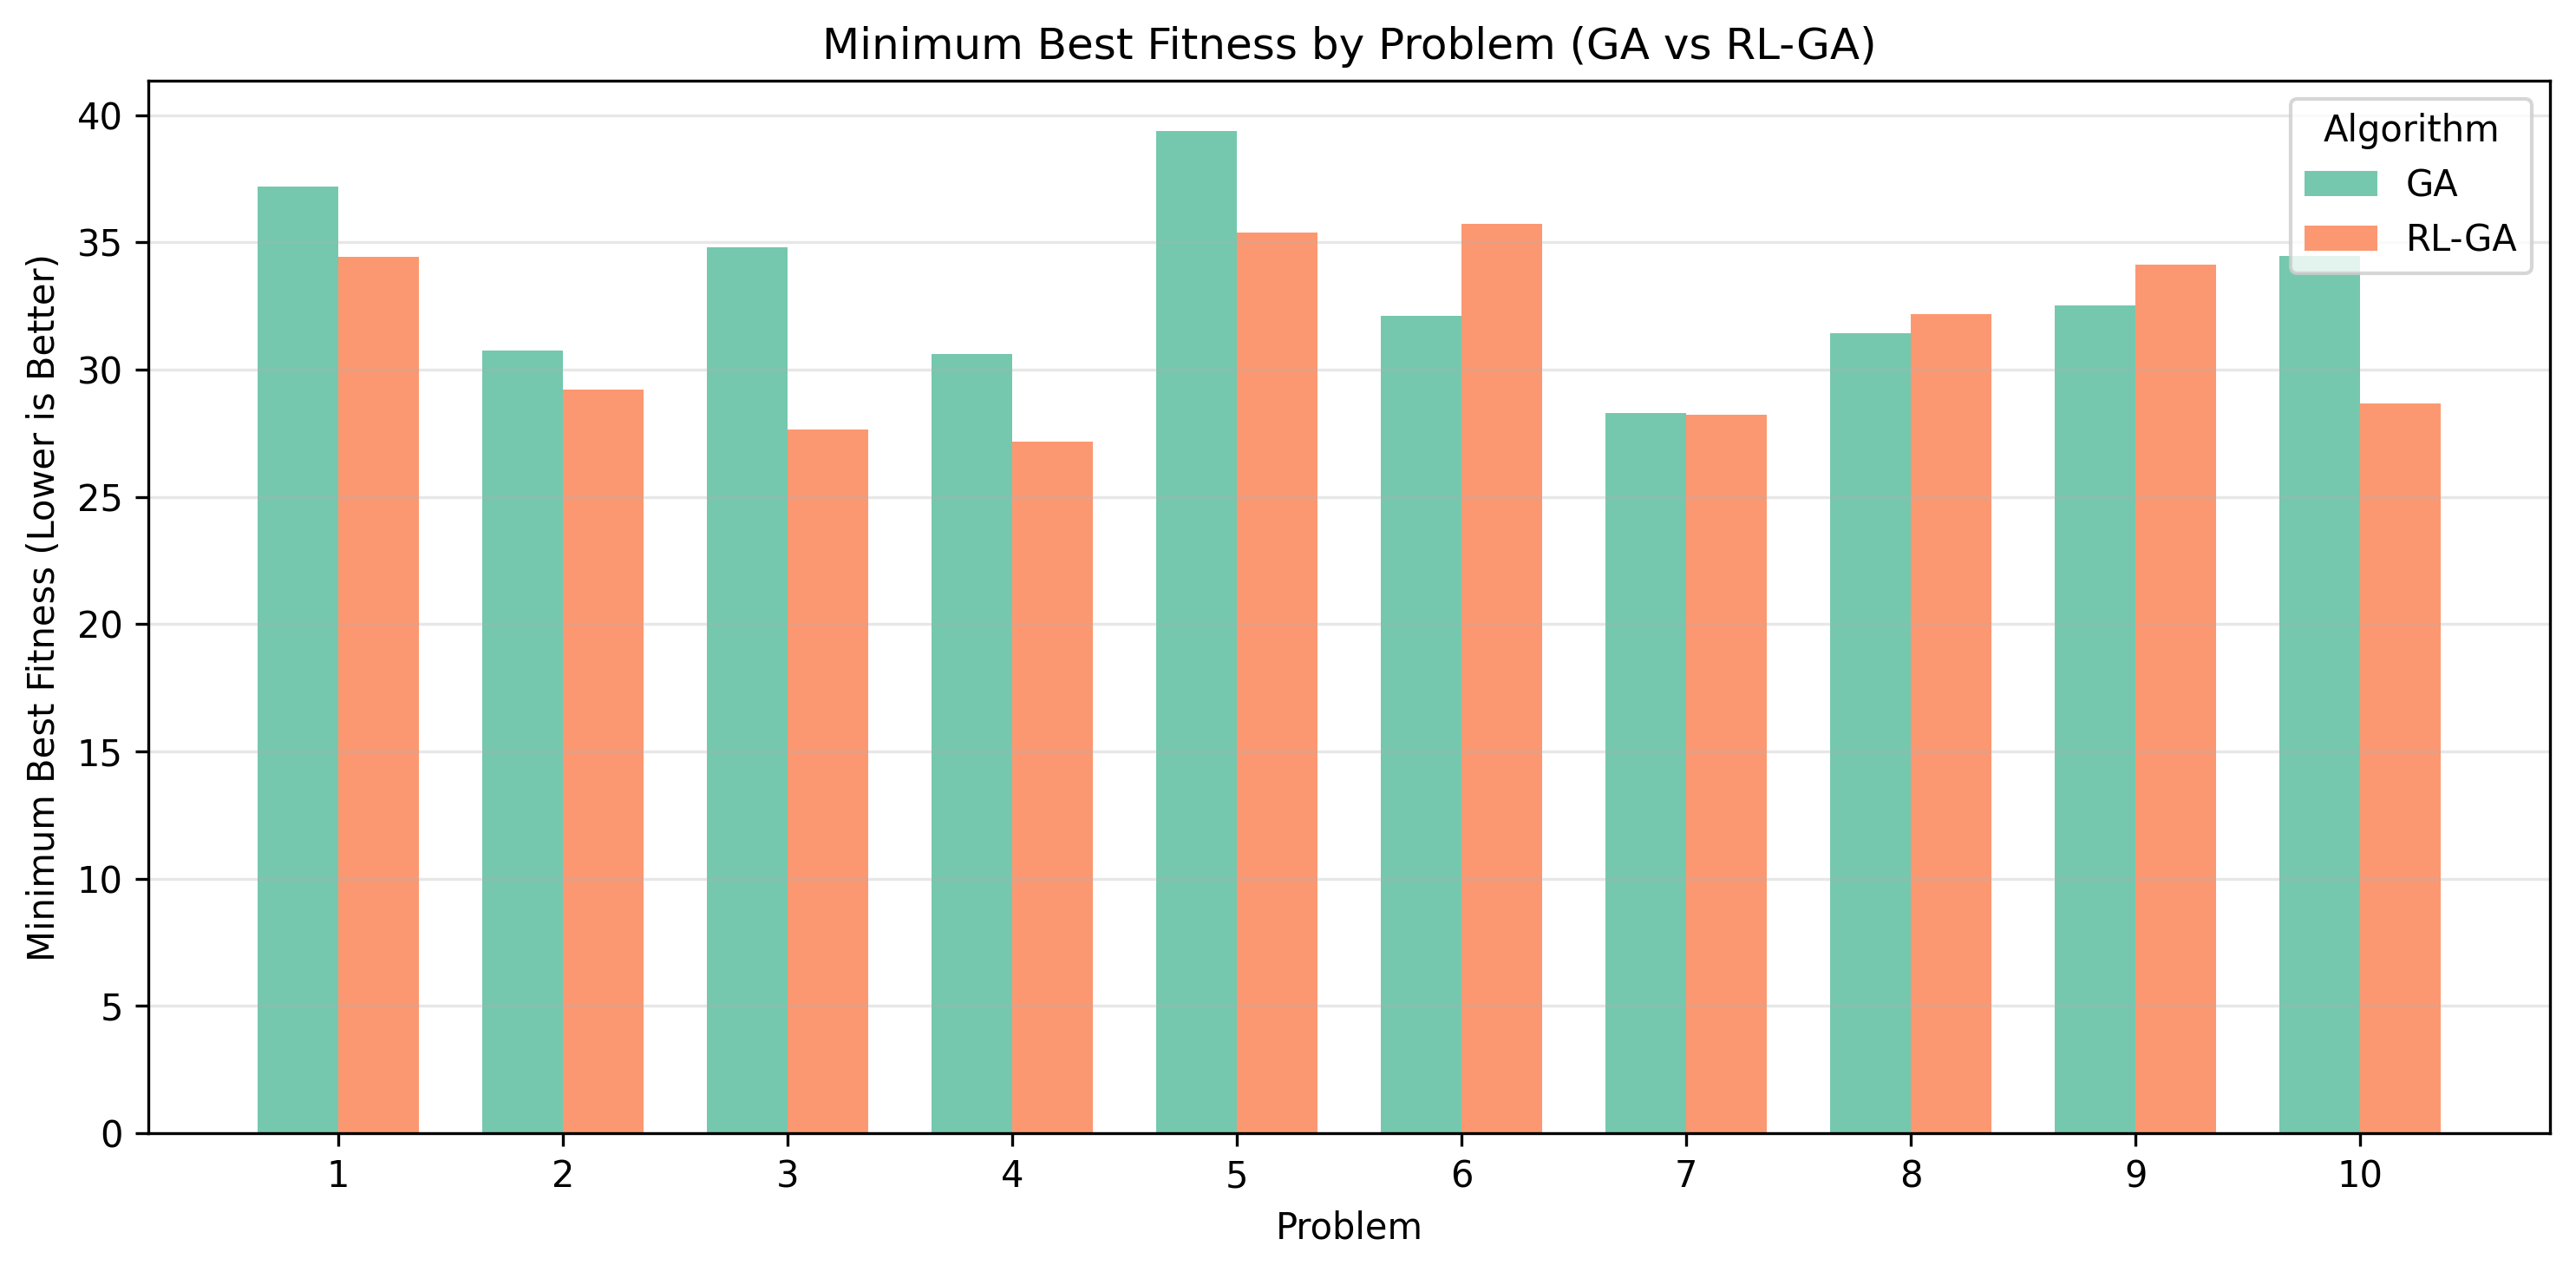
\includegraphics[width=0.67\linewidth]{results_500_300_8/best_fitness_min.png}
    \caption{Line plot of best fitness range for 10 random problems for standard GA and RL-GA Agent 1}
    \label{fig:placeholder}
\end{figure}
\begin{figure}[H]
    \centering
    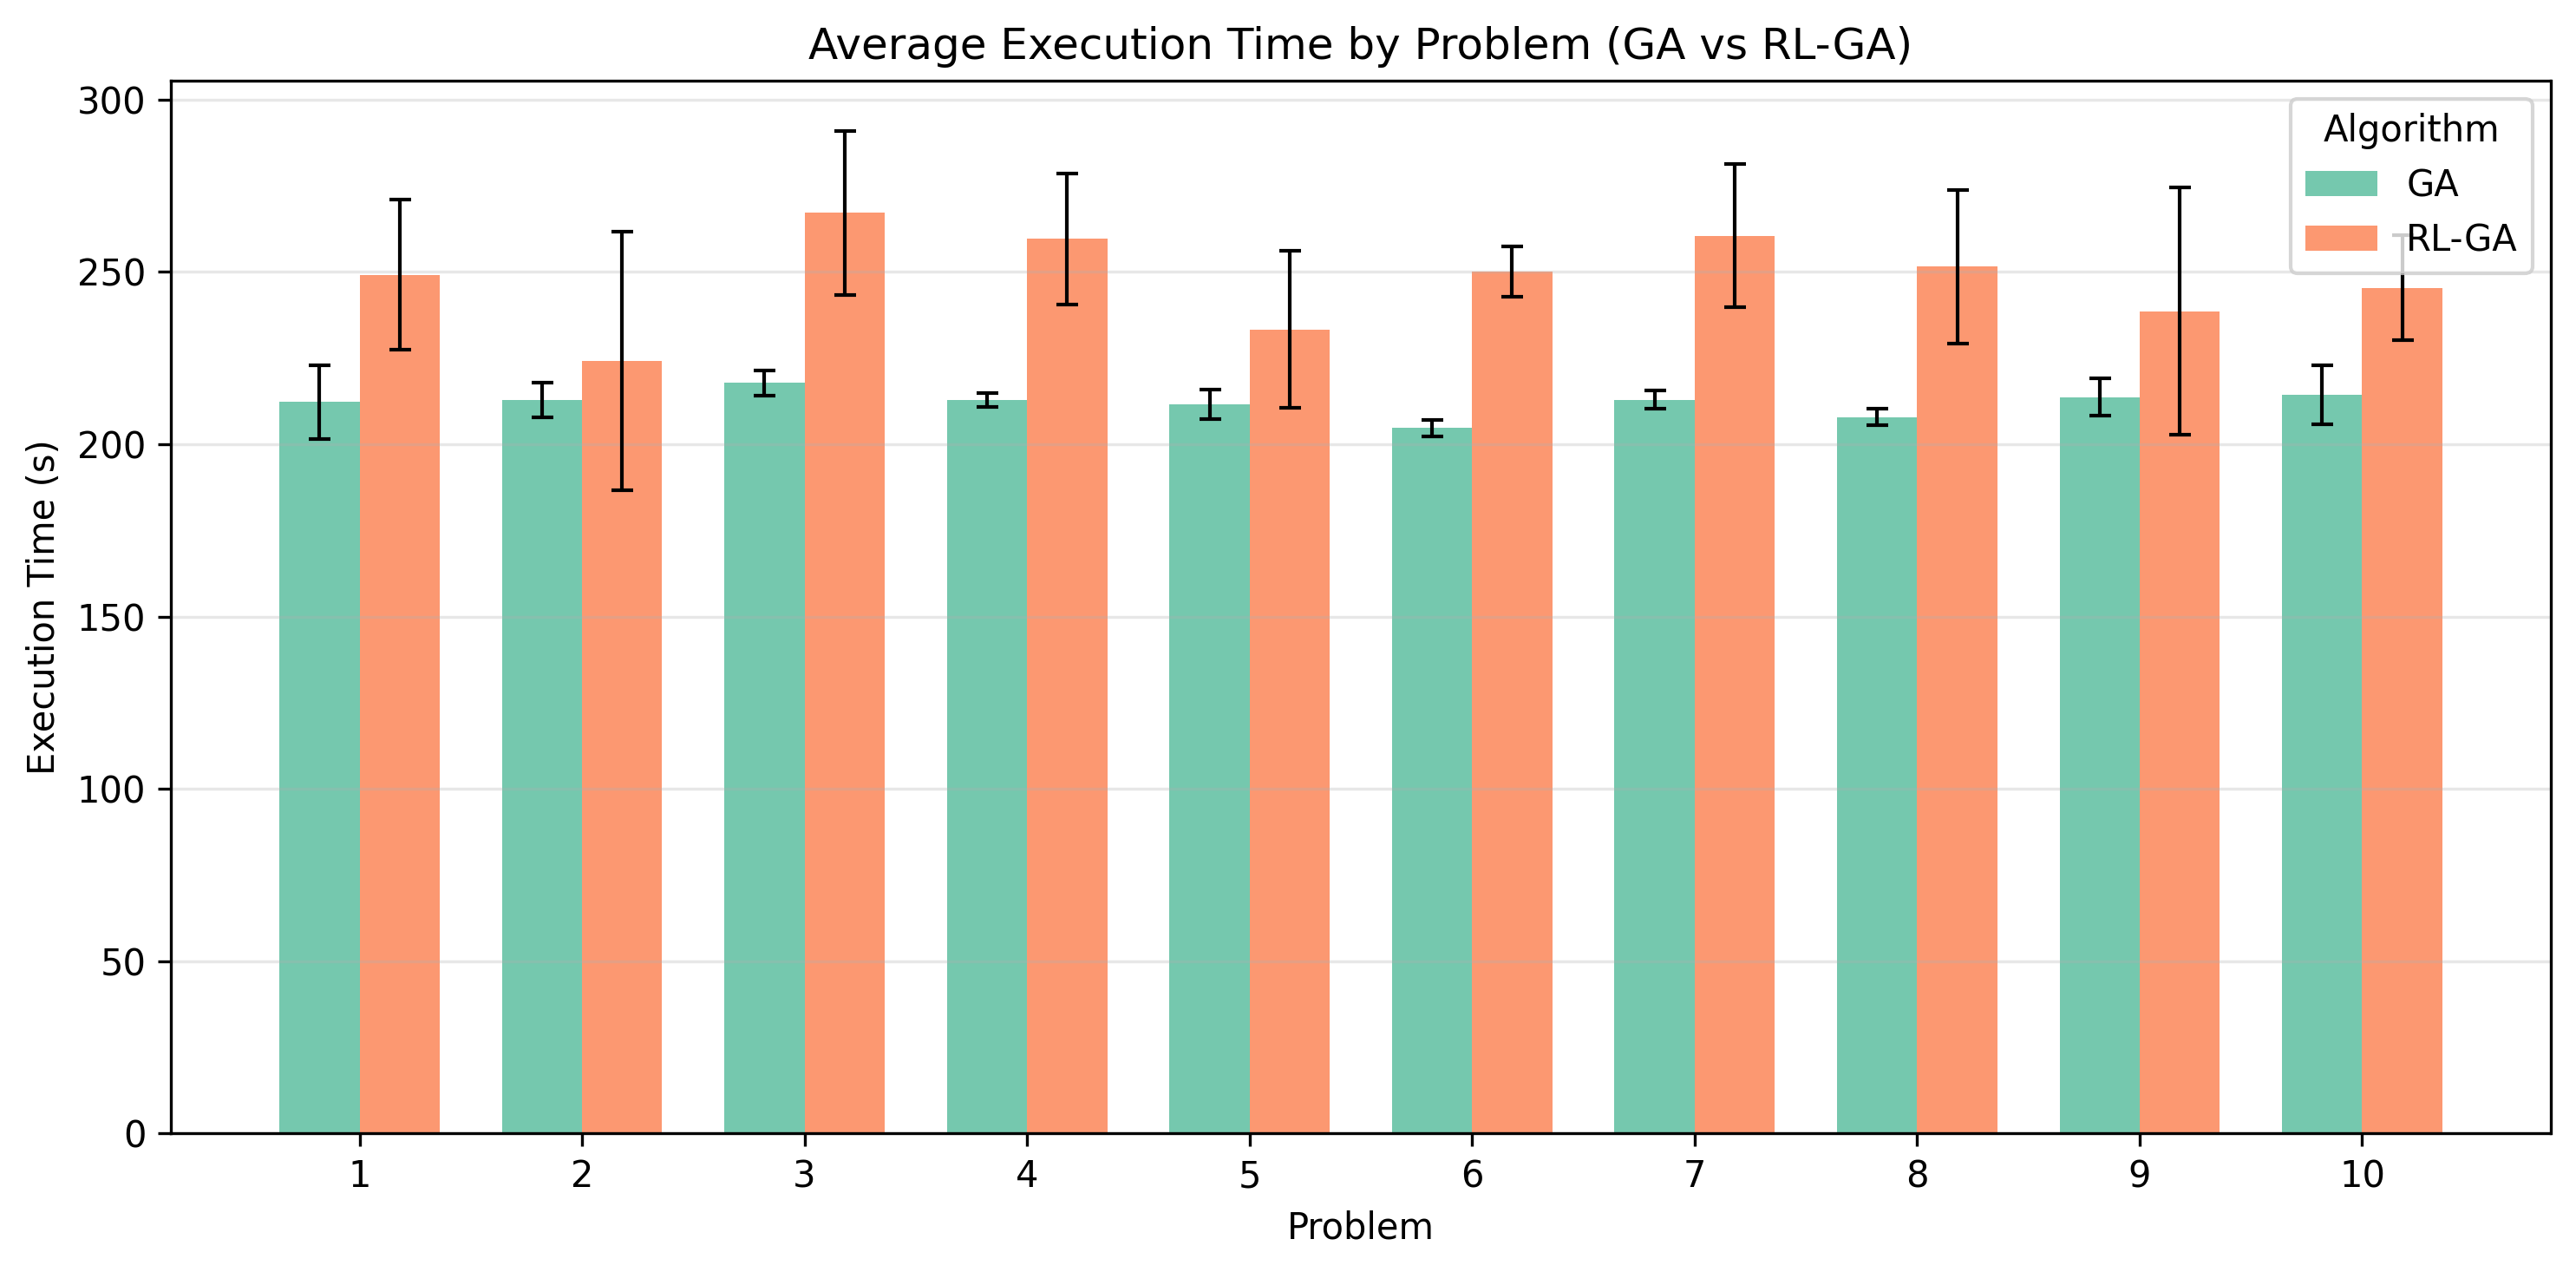
\includegraphics[width=0.67\linewidth]{results_500_300_8/execution_time_avg.png}
    \caption{Bar plot of average execution time for 10 random problems for standard GA and RL-GA Agent 1}
    \label{fig:placeholder}
\end{figure}
\subsubsection{Performance Comparison}
Table \ref{tab:problem_comparison_rlga1} summarizes the performance metrics (average best fitness, best best fitness, average total distance, execution time) comparisons of Problems 1 to 10 for both standard GA and RL-GA Agent 1.
\begin{table}[H]
\centering
\small
\begin{tabular}{lcccccccc}
\toprule
& \multicolumn{4}{c}{\textbf{GA}} & \multicolumn{4}{c}{\textbf{RL-GA Agent 1}} \\
\cmidrule(lr){2-5} \cmidrule(lr){6-9}
\textbf{Problem} & \textbf{Avg Fit} & \textbf{Best Fit} & \textbf{Avg Dist} & \textbf{Time (s)}
& \textbf{Avg Fit} & \textbf{Best Fit} & \textbf{Avg Dist} & \textbf{Time (s)} \\
\midrule
1  & 38.2674 & 37.1987 & 36.6903 & 212.2843 & 37.4578 & 34.4459 & 36.0842 & 249.1539 \\
2  & 31.7253 & 30.7442 & 30.1939 & 212.7693 & 33.3297 & 29.2128 & 31.9496 & 224.1780 \\
3  & 34.9526 & 34.8201 & 33.2508 & 217.8172 & 32.9599 & 27.6629 & 31.4589 & 267.1172 \\
4  & 32.6156 & 30.6245 & 31.2394 & 212.8344 & 28.4347 & 27.1720 & 26.9106 & 259.6510 \\
5  & 40.4657 & 39.3870 & 38.8144 & 211.4782 & 38.3585 & 35.4029 & 36.6992 & 233.3397 \\
6  & 35.1953 & 32.1232 & 33.6237 & 204.7021 & 37.1586 & 35.7327 & 35.4922 & 250.0660 \\
7  & 32.7923 & 28.3086 & 31.3092 & 212.9213 & 32.4510 & 28.2172 & 30.8057 & 260.5010 \\
8  & 35.8083 & 31.4425 & 34.0846 & 207.9091 & 34.9034 & 32.1993 & 33.1182 & 251.5820 \\
9  & 35.7369 & 32.5320 & 34.0767 & 213.6882 & 35.7402 & 34.1358 & 34.3652 & 238.6408 \\
10 & 34.9946 & 34.4798 & 33.5108 & 214.3778 & 30.0047 & 28.6878 & 28.6114 & 245.3618 \\
\midrule
\textbf{Average} & 35.2554 & 33.1661 & 33.6794 & 212.0782 & 34.0799 & 31.2869 & 32.5495 & 247.9591 \\
\bottomrule
\end{tabular}
\caption{Performance comparison of GA and RL-GA Agent 1 across 10 benchmark problems.}
\label{tab:problem_comparison_rlga1}
\end{table}

\textbf{Average Best Fitness} \newline
From Problems 1 to 10, RL-GA Agent 1 achieved a better average best fitness in 7/10 problems (Problems 1, 3, 4, 5, 7, 8, 10), while GA got better average best fitness in 3/10 problems (Problems 2, 6, 9). RL-GA Agent 1 was observed to improve the average best fitness from 35.26 (GA) to 34.08 (RL-GA Agent 1) on average across the 10 problems (3.3\% improvement). The largest improvement occurred in Problem 10 with a 14.3\% improvement in average best fitness, whereas the largest degradation occurs in Problem 6 where RL-GA was 5.6\% worse than standard GA.

\textbf{Minimum Best Fitness} \newline
Considering best-case performance, RL-GA Agent 1 achieved a lower minimum best fitness in 7/10 problems (Problems 1, 2, 3, 4, 5, 7, 10), while GA obtained better best-case fitness in 3/10 problems (Problems 6, 8, 9). On average, the best best fitness improves from 33.17 (GA) to 31.29 (RL-GA Agent 1) across the 10 problems (5.7\% improvement). The largest improvement occurred in Problem 3, where RL-GA achieves a 20.6\% better best-case fitness, while the largest degradation occurred in Problem 6, where RL-GA is 11.2\% worse than standard GA.

\textbf{Execution Time} \newline
From Problems 1 to 10, RL-GA Agent 1 took higher execution time in all 10 problems compared to standard GA. In detail, RL-GA Agent 1 increased the average execution time from 212.1 s (GA) to 248.0 s (16.9\% increase). The largest increase was observed in Problem 3 with a 22.6\% increase, while the smallest increase occurred in Problem 2 with an approximate 5.4\% increase.

\textbf{Summary} \newline
\begin{table}[H]
\centering
\small
\begin{tabular}{lccc}
\toprule
\textbf{Metric} & \textbf{GA} & \textbf{RL-GA Agent 1} & \textbf{Change \%} \\
\midrule
Average Best Fitness   & 35.2554 & 34.0799 & $-3.33\%$ \\
Best Best Fitness      & 33.1661 & 31.2869 & $-5.67\%$ \\
Execution time (s)     & 212.0782 & 247.9591 & $+16.92\%$ \\
\bottomrule
\end{tabular}
\caption{Overall key metrics summary of GA vs RL-GA Agent 1}
\label{tab:overall_summary}
\end{table}

Table \ref{tab:overall_summary} shows the overall summary of standard GA and RL-GA Agent 1 averaged from Problem 1 to Problem 10. A negative change implies better results for both average and best best fitness. However, execution time marked a positive change, which meant a slower time to reach the same number of generations.

\newpage
\section{Results: GA vs RL-GA Agent 2}
In this results section, RL-GA Agent 2 is trained through 15 different problems with population size of 200, and generation number of 300. RL-GA Agent 2 was compared with two different standard GA settings, one with default parameter values (10\% LS), and the other with guaranteed local search settings (100\% LS).

\subsection{Sample Problem}
The same problem as stated in Section 8.1 was used again for this sample problem comparison for standard GA and RL-GA Agent 2 experiment. The sample problem was solved with RL-GA Agent 2, and with the same standard GA parameter settings in the previous results (Chapter 9), where the local search rate is 10\%. For sample problem sections, the exploration rate $\epsilon$ is set to zero to make full use of the knowledge learned from the RL agent, which may be useful for more clean analysis.
\subsubsection{RL-GA Parameter Control}
\begin{figure}[H]
    \centering
    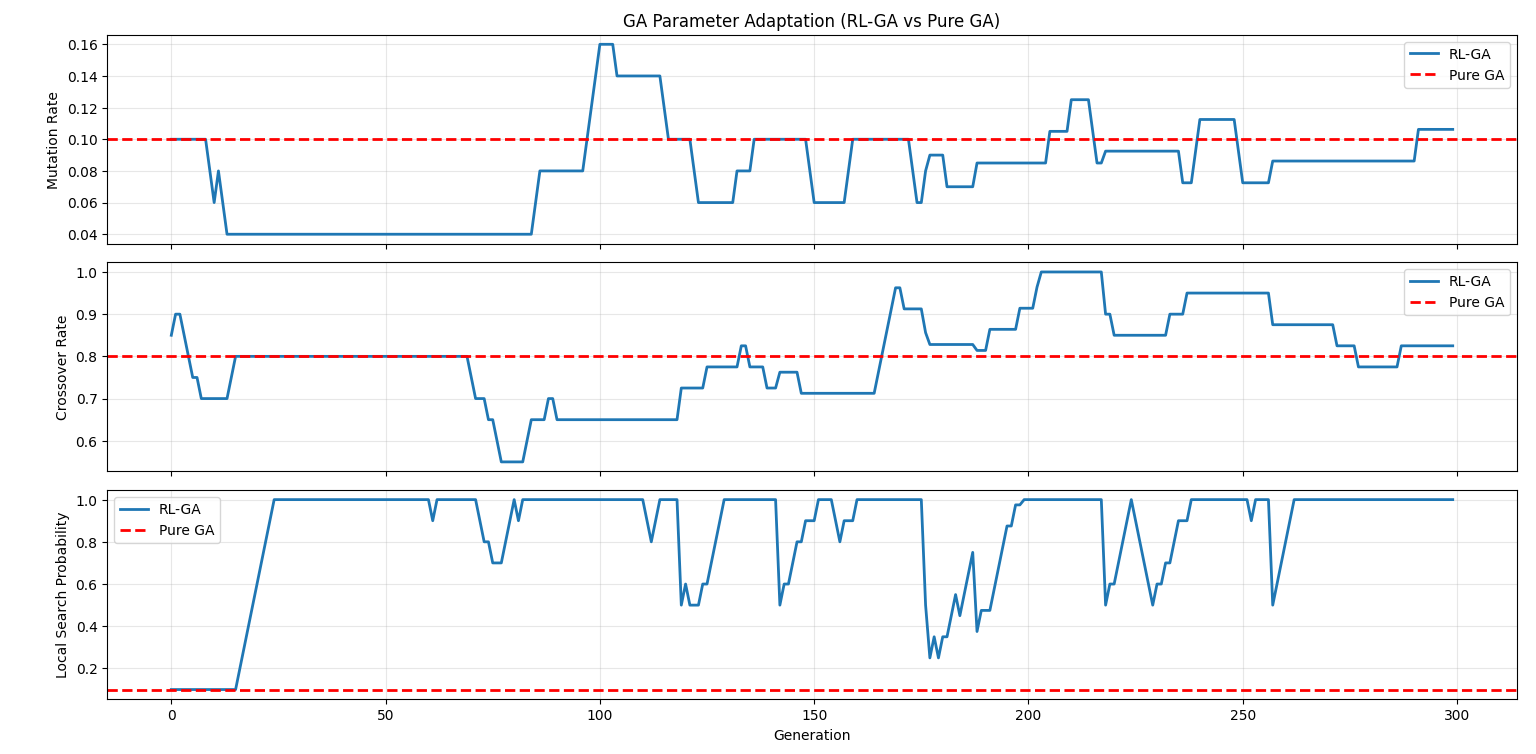
\includegraphics[width=1\linewidth]{pure_ga_vs_agent_2_sample/parametergraph.png}
    \caption{GA parameter values due to RL-GA Agent 2 adaptive actions against the number of generations}
    \label{fig:sample_rl_vs_ga_parameters_2}
\end{figure}
Figure \ref{fig:sample_rl_vs_ga_parameters_2} shows the GA parameter values through the dynamic control of RL-GA Agent 2, compared to the static standard GA settings. The mutation rate decreased during early generations down to a minimum value of 0.04, and gradually increased in later generations, where it reached a maximum value of 0.16 after generation 100, but later oscillated around the default value. The crossover rate shows a rather adaptive behavior throughout the generations, where it increased progressively and reached values close to 1.0 in later generations. Lastly, the local search probability began to escalate rapidly from early generations, reaching a value of 1.0 around generation 24 and remaining high for a sustained range of generations before slightly fluctuating towards later generations.

\subsubsection{Optimized Layout Comparison}
\begin{figure}[H]
    \centering
    \begin{subfigure}{0.48\linewidth}
        \centering
        
\includegraphics[width=\linewidth]{pure_ga_vs_agent_2_sample/rl_optimized_layout.png}
        \caption{RL-GA Agent 2 optimized layout}
    \end{subfigure}
    \hfill
    \begin{subfigure}{0.48\linewidth}
        \centering
        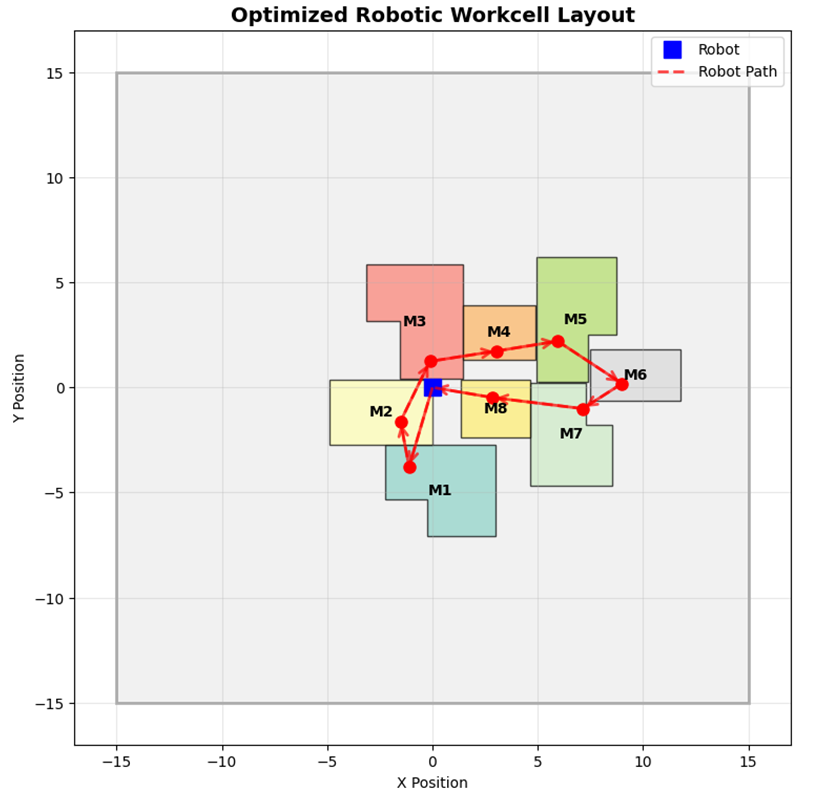
\includegraphics[width=\linewidth]{pure_ga_vs_agent_1_sample/ga_optimized_layout.png}
        \caption{Standard GA optimized layout}
    \end{subfigure}
    
    \caption{Comparison of optimization performance and resulting layouts for the sample problem}
    \label{fig:rl_ga_comparison_2}
\end{figure}
\begin{table}[H]
\centering
\small
\setlength{\tabcolsep}{6pt}
\renewcommand{\arraystretch}{1.2}
\begin{tabular}{c c c c c c c}
\toprule
\multirow{2}{*}{\textbf{Machine}} 
& \multicolumn{3}{c}{\textbf{Standard GA}} 
& \multicolumn{3}{c}{\textbf{RL-GA Agent 2}} \\
\cmidrule(lr){2-4} \cmidrule(lr){5-7}
& \textbf{X} & \textbf{Y} & \textbf{Rot ($^\circ$)} 
& \textbf{X} & \textbf{Y} & \textbf{Rot ($^\circ$)} \\
\midrule
1 & 0.37  & -4.90 & 180 & -1.93 & -3.57 & 90 \\
2 & -2.44 & -1.17 & 0   & -2.44 & 0.60  & 0 \\
3 & -0.84 & 3.13  & 180 & -0.10 & 4.90  & 180 \\
4 & 3.19  & 2.62  & 180 & 3.49  & 3.61  & 270 \\
5 & 6.82  & 3.24  & 270 & 6.68  & 4.01  & 270 \\
6 & 9.63  & 0.59  & 0   & 5.98  & -0.20 & 0 \\
7 & 6.59  & -2.23 & 0   & 3.12  & -3.32 & 0 \\
8 & 3.01  & -1.00 & 180 & 1.64  & 0.51  & 0 \\
\bottomrule
\end{tabular}
\caption{Comparison of machine configurations between Standard GA (Fitness = 30.01) and RL-GA Agent 2 (Fitness = 29.12)}
\label{tab:ga_vs_rlga_layout_2}
\end{table}
\vspace{-25pt}
Figure \ref{fig:rl_ga_comparison_2} shows the finalized layout from the standard GA and RL-GA Agent 2 computation for 300 generations. The standard GA achieves the best fitness of 30.01, while the RL-GA Agent 2 achieves the best fitness of 29.12, which is 3\% better than standard GA. Table \ref{tab:ga_vs_rlga_layout_2} summarizes the machines' global locations and final rotations that correspond to Figure \ref{fig:rl_ga_comparison_2}.
\subsubsection{Fitness Convergence}
\begin{figure}[H]
    \centering
    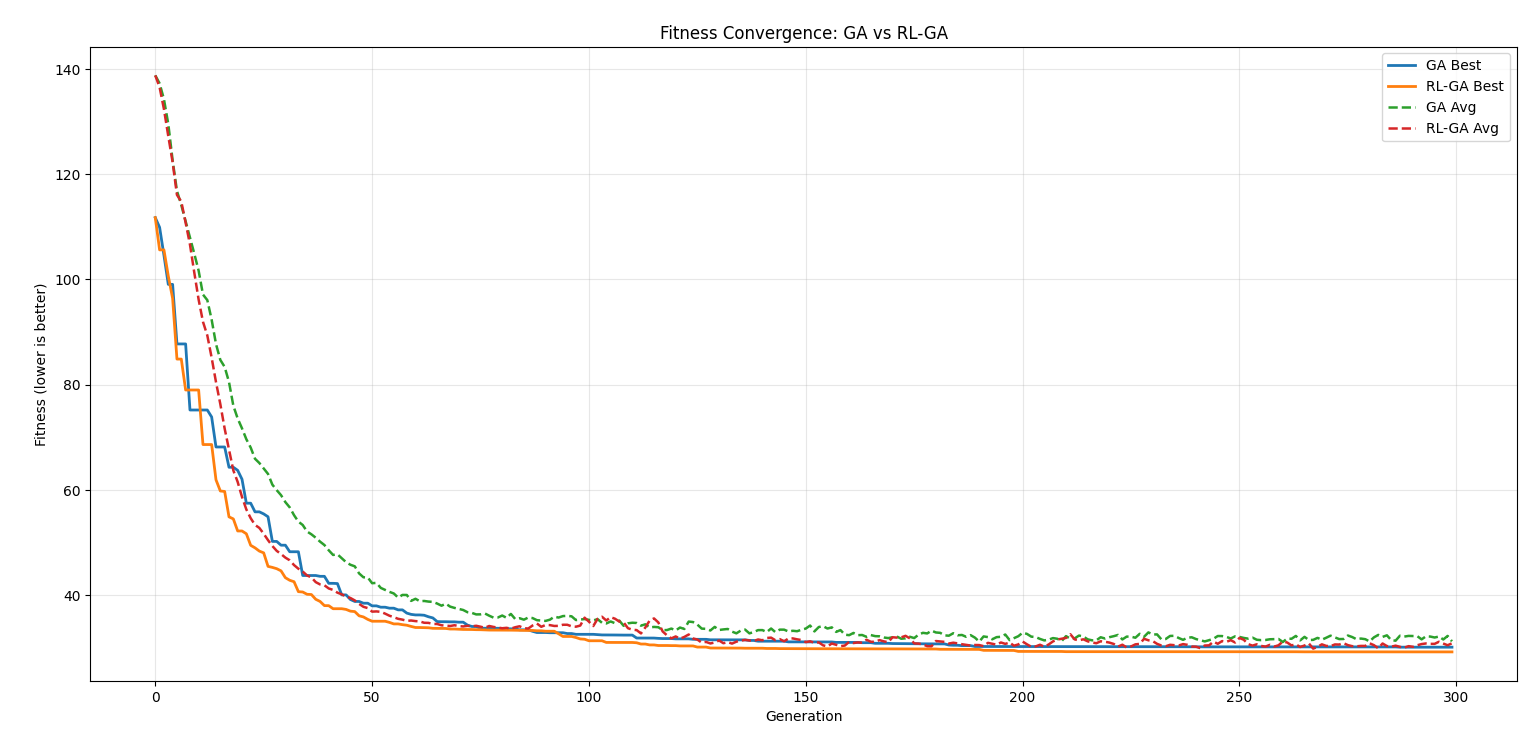
\includegraphics[width=0.8\linewidth]{pure_ga_vs_agent_2_sample/fitness_convergence.png}
    \caption{Fitness convergence graph comparison of sample problem for standard GA and RL-GA Agent 2}
    \label{fig:placeholder}
\end{figure}
\begin{table}[H]
\centering
\begin{tabular}{ccccccc}
\toprule
\textbf{Generation} & \textbf{Algorithm} & \textbf{Best Fitness} & \textbf{Average Fitness} & \textbf{Diversity} \\
\midrule
0   & Standard GA & 111.77 & 138.85 & 416.098 \\
0   & RL-GA   & 111.77 & 138.85 & 416.098 \\
\midrule
60  & Standard GA & 36.15  & 39.23  & 208.382 \\
60  & RL-GA   & 33.76  & 34.98  & 90.18 \\
\midrule
120 & Standard GA & 31.60  & 33.21  & 165.909 \\
120 & RL-GA   & 30.31  & 32.06  & 299.00 \\
\midrule
180 & Standard GA & 30.64  & 32.81  & 176.715 \\
180 & RL-GA   & 29.67  & 31.18  & 149.75 \\
\midrule
240 & Standard GA & 30.08  & 31.55  & 161.184 \\
240 & RL-GA   & 29.15  & 30.11  & 273.39 \\
\midrule
300 & Standard GA & 30.01  & 30.93  & 134.044 \\
300 & RL-GA   & 29.12  & 30.76  & 176.17 \\
\bottomrule
\end{tabular}
\caption{Fitness and diversity comparison between standard GA and RL-GA Agent 2 at selected generations}
\label{tab:ga_rlga_2_sample_problem}
\end{table}
\vspace{-25pt}
Table \ref{tab:ga_rlga_2_sample_problem} shows the fitness evolution for increments of 60 generations. At earlier generations, RL-GA Agent 2 converged faster than the standard GA, where the diversity is also shown to be much lower than the standard GA at generation 60. In later generations, RL-GA Agent 2 remained broadly on par with standard GA in convergence trend, while maintaining a slightly better best fitness until the end of the run. For the execution time, GA reached 300 generations for 218.94 seconds while RL-GA Agent 2 for 295.04 seconds (34.76\% longer).

\subsection{Experiment with 10 Problems}
Standard GA was tested with two different settings, one with a local search (LS) rate of 10\%, and the other with an LS rate of 100\%. Then, these two GAs were compared with the same RL-GA agent. However, since these were stochastic processes, RL-GA Agent 2 had different values compared to 10\% and 100\% LS standard GA, although the agent uses the same Q-table. For fairness, the values of RL-GA Agent 2 were averaged, meaning that the number of runs of RL-GA Agent 2 were technically twice the number of runs of the standard GAs (number of runs = 3). The raw values of RL-GA were summarized in the Appendix. 
\subsubsection{Figures}
\begin{figure}[H]
    \centering
    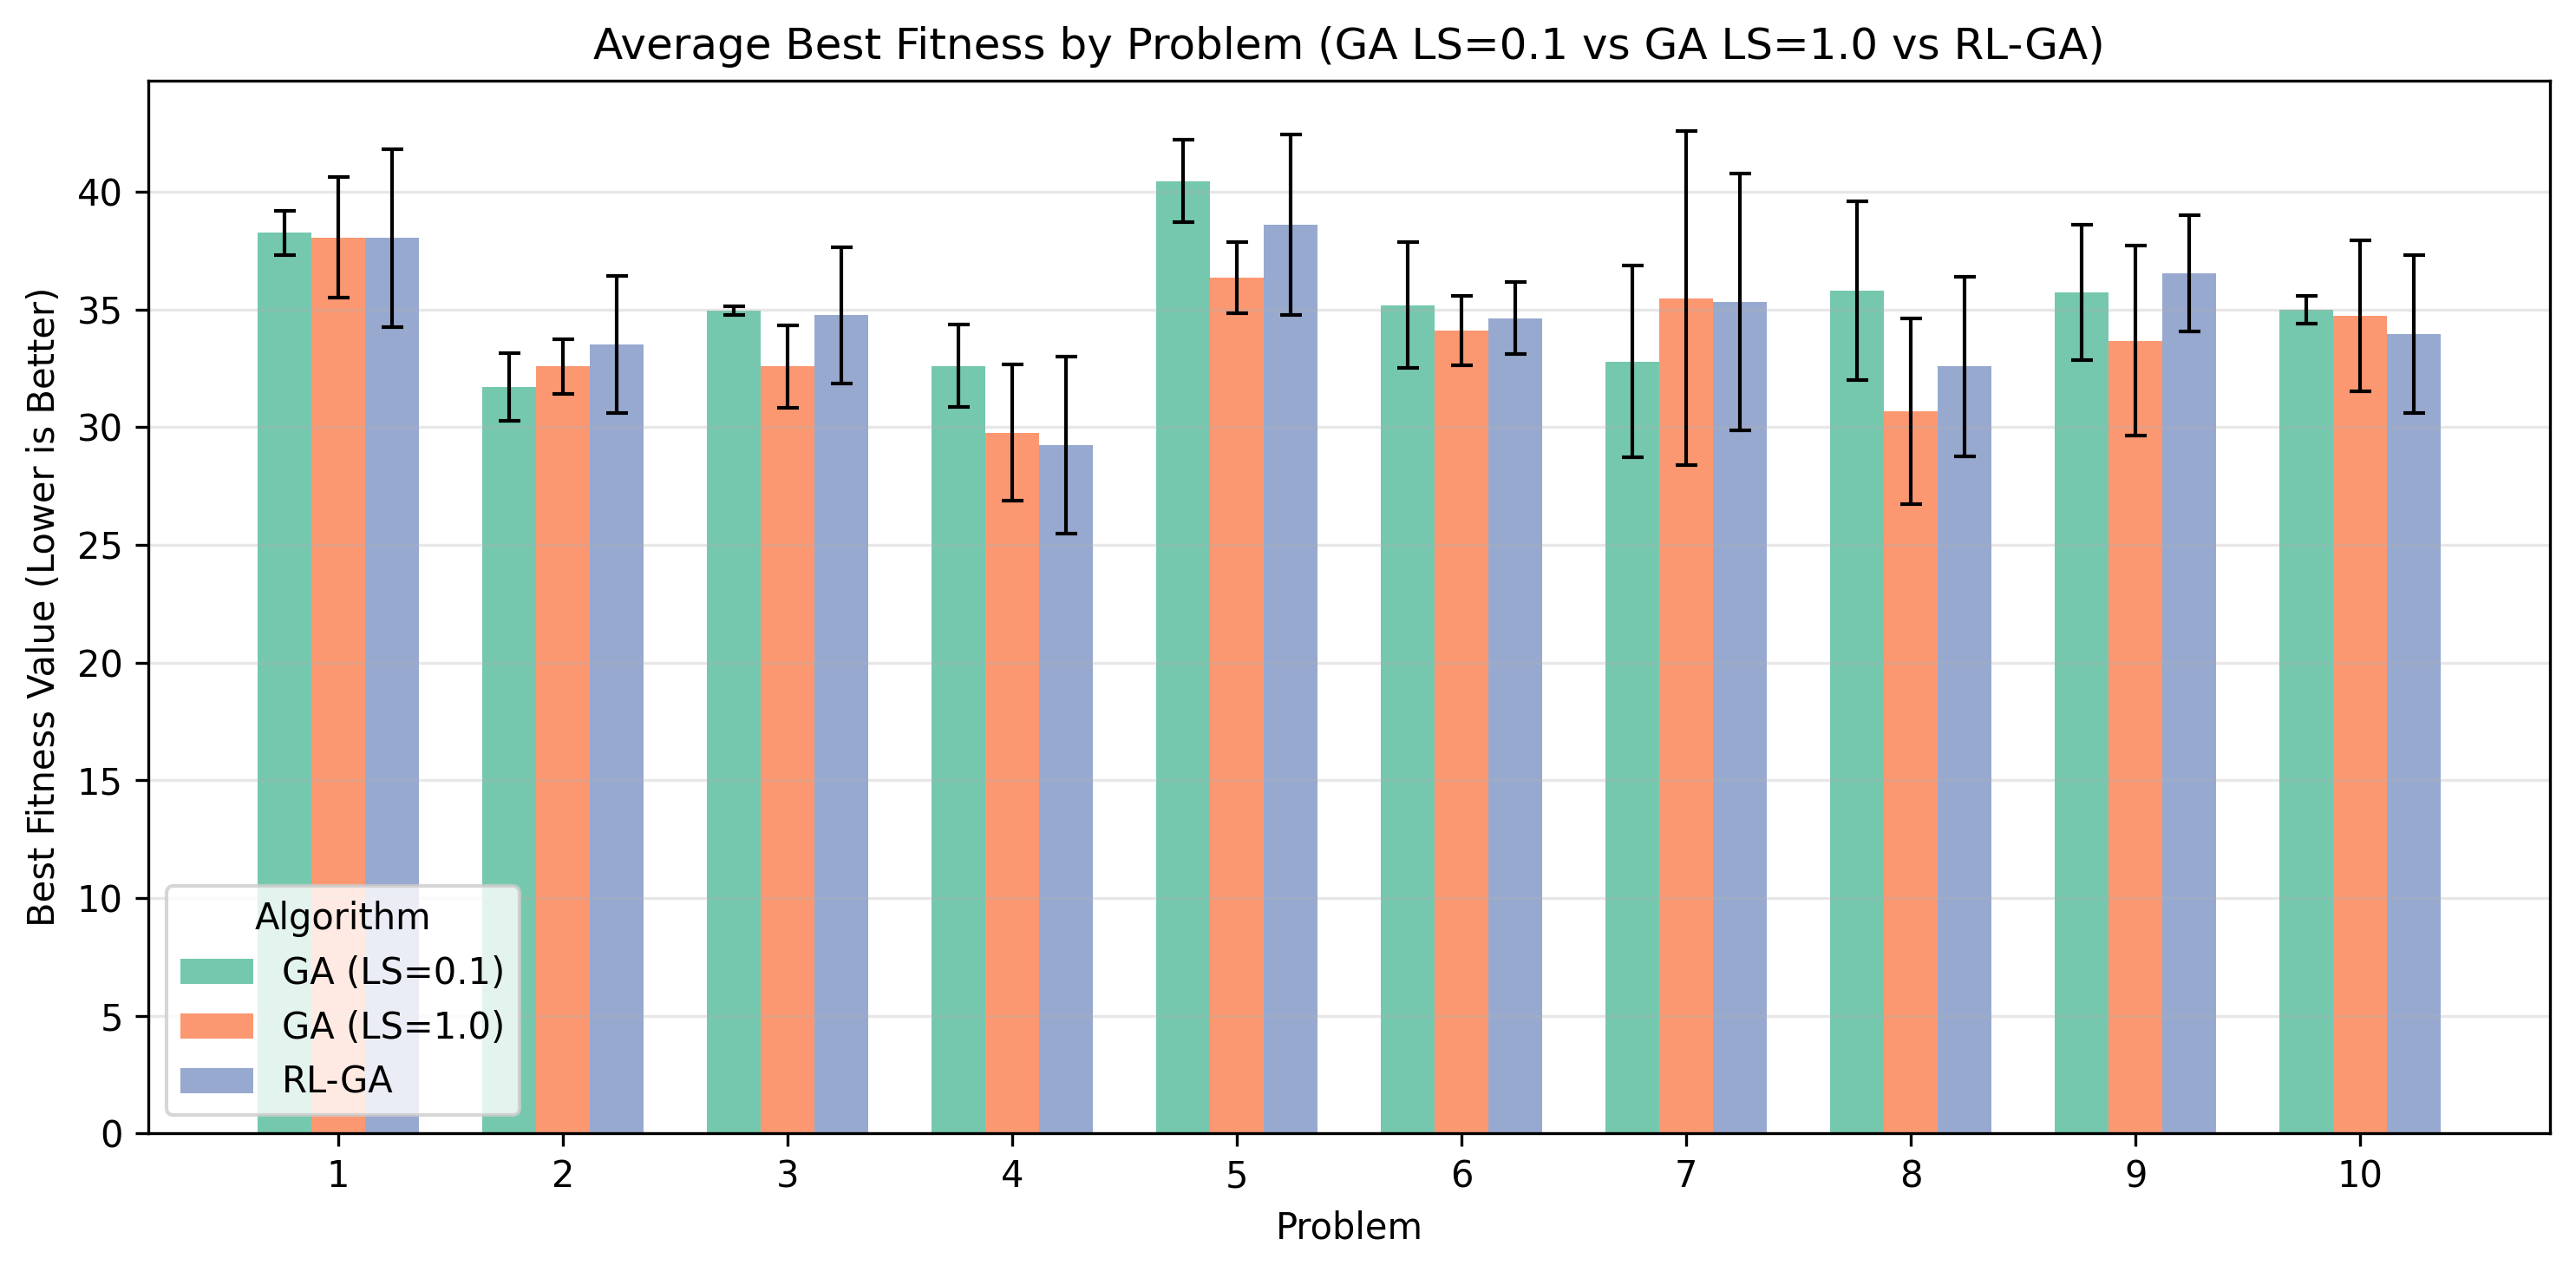
\includegraphics[width=0.67\linewidth]{plots_3algs/comparison_plots/average_best_fitness.png}
    \caption{Bar plot of average best fitness for 10 random problems for standard GA (10\% and 100\% LS) and RL-GA (averaged) agent 2}
    \label{fig:placeholder}
\end{figure}
\vspace{-25pt}
\begin{figure}[H]
    \centering
    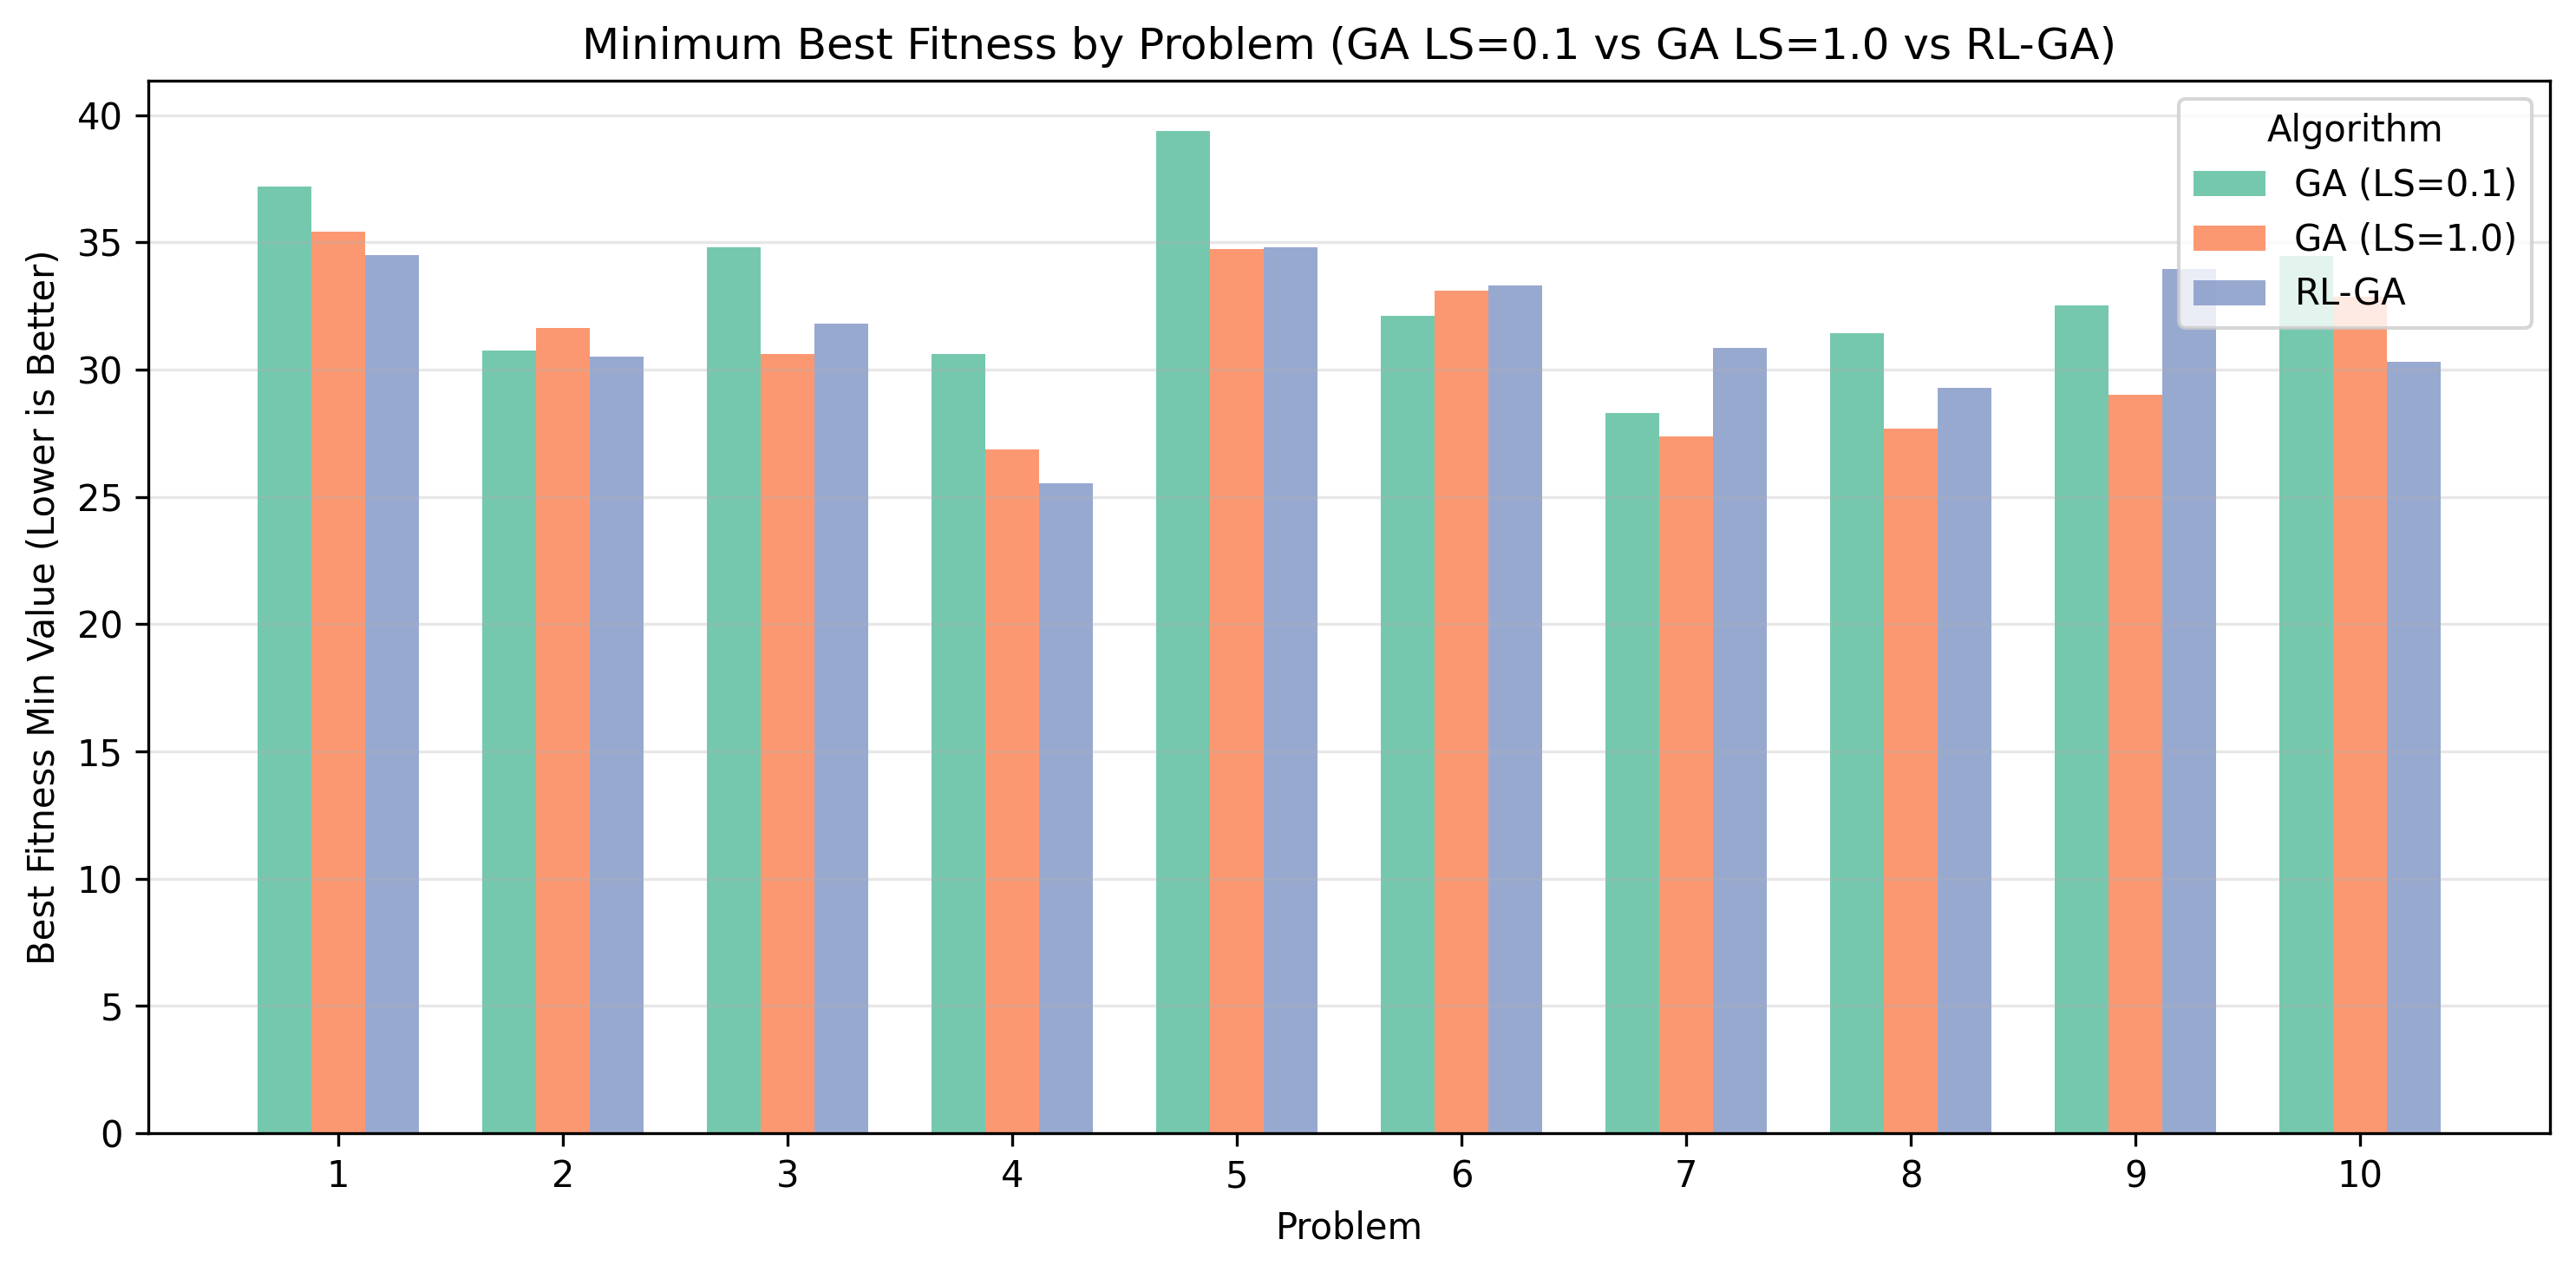
\includegraphics[width=0.67\linewidth]{plots_3algs/comparison_plots/minimum_best_fitness.png}
    \caption{Bar plot of minimum best fitness for 10 random problems for standard GA (10\% and 100\% LS) and RL-GA (averaged) Agent 2}
    \label{fig:placeholder}
\end{figure}
\vspace{-25pt}
\begin{figure}[H]
    \centering
    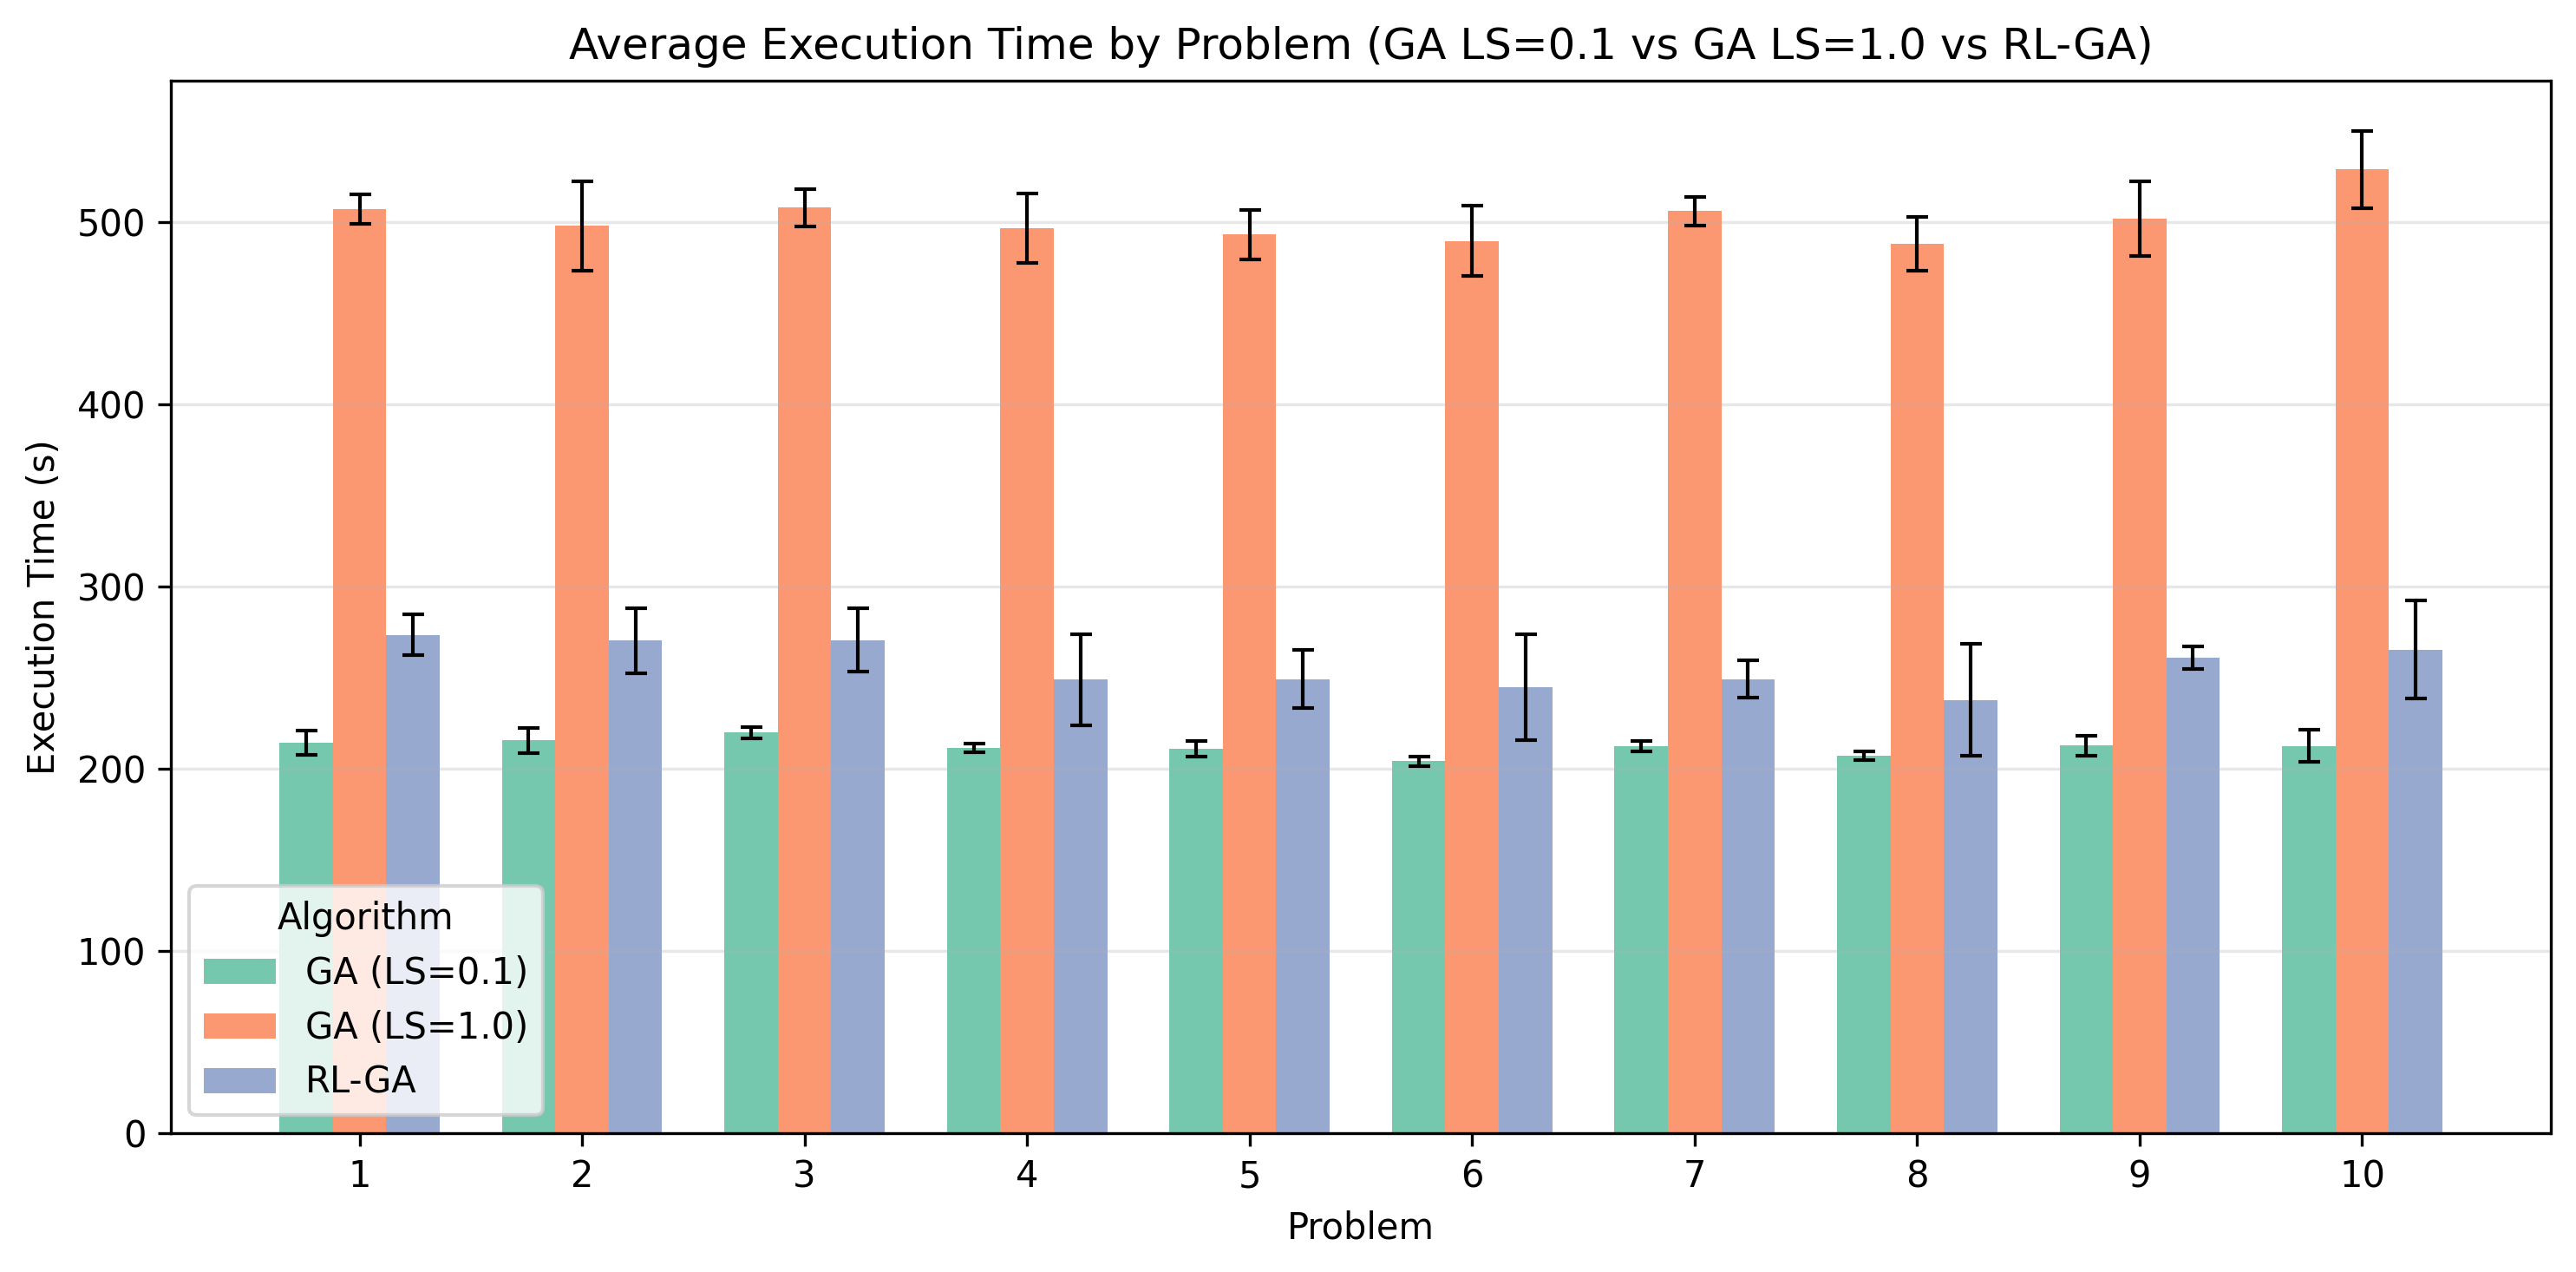
\includegraphics[width=0.67\linewidth]{plots_3algs/comparison_plots/execution_time.png}
    \caption{Bar plot of average execution time for 10 random problems for standard GA (10\% and 100\% LS) and RL-GA (averaged) Agent 2}
    \label{fig:placeholder}
\end{figure}
\subsubsection{Performance Comparison (vs 10\% LS)}
Table \ref{tab:rlga_ga10_corrected} summarizes the performance comparison metric of RL-GA Agent 2, compared to the standard genetic algorithm with a default 10\% local search rate, i.e. 10\% chance of doing local search on elites per generation. The average best fitness, minimum best fitness and execution time are discussed as below.
\begin{table}[H]
\centering
\small
\begin{tabular}{lcccccccc}
\toprule
& \multicolumn{4}{c}{\textbf{GA (10\% LS)}} & \multicolumn{4}{c}{\textbf{RL-GA Agent 2}} \\
\cmidrule(lr){2-5} \cmidrule(lr){6-9}
\textbf{Problem} & \textbf{Avg Fit} & \textbf{Best Fit} & \textbf{Avg Dist} & \textbf{Time (s)}
& \textbf{Avg Fit} & \textbf{Best Fit} & \textbf{Avg Dist} & \textbf{Time (s)} \\
\midrule
1  & 38.2674 & 37.1987 & 36.6903 & 214.3672 & 38.0538 & 34.4927 & 36.4279 & 273.5278 \\
2  & 31.7253 & 30.7442 & 30.1939 & 215.4668 & 33.5166 & 30.5137 & 31.9044 & 270.3908 \\
3  & 34.9526 & 34.8201 & 33.2508 & 219.8142 & 34.7571 & 31.8035 & 33.1966 & 270.6215 \\
4  & 32.6156 & 30.6245 & 31.2394 & 211.3244 & 29.2389 & 25.5366 & 27.7646 & 248.9127 \\
5  & 40.4657 & 39.3870 & 38.8144 & 210.9599 & 38.6065 & 34.8212 & 37.0278 & 249.2543 \\
6  & 35.1953 & 32.1232 & 33.6237 & 204.0816 & 34.6422 & 33.3020 & 33.2177 & 244.7214 \\
7  & 32.7923 & 28.3086 & 31.3092 & 212.3251 & 35.3143 & 30.8591 & 33.6927 & 249.1416 \\
8  & 35.8083 & 31.4425 & 34.0846 & 207.0846 & 32.5873 & 29.2781 & 30.9226 & 237.7813 \\
9  & 35.7369 & 32.5320 & 34.0767 & 212.6961 & 36.5325 & 33.9700 & 34.9855 & 260.9053 \\
10 & 34.9946 & 34.4798 & 33.5108 & 212.5281 & 33.9630 & 30.3058 & 32.5136 & 265.2834 \\
\midrule
\textbf{Average} & 35.2554 & 33.1661 & 33.6794 & 212.0648 & 34.7212 & 31.4883 & 33.1653 & 257.0540 \\
\bottomrule
\end{tabular}
\caption{Performance comparison of Standard GA (10\% LS) and RL-GA Agent 2 (averaged) across 10 benchmark random problems.}
\label{tab:rlga_ga10_corrected}
\end{table}
\textbf{Average Best Fitness} \newline
From Problems 1 to 10, RL-GA Agent 2 achieved a better average best fitness in 7/10 problems (Problems 1, 3, 4, 5, 6, 8, and 10). RL-GA Agent 2 was observed to improve the average best fitness from 35.2554 to 34.7212 on average across the 10 problems (1.5\% improvement). The largest improvement occurred in Problem 4 with a 10.4\% improvement in average best fitness.

\textbf{Minimum Best Fitness} \newline
Considering best-case performance, RL-GA Agent 2 achieved a lower minimum best fitness in 7/10 problems (Problems 1, 2, 3, 4, 5, 8, and 10). On average, the best minimum fitness improves from 33.1661 (GA) to 31.4883 (RL-GA Agent 2) across the 10 problems (5.1\% improvement). The largest improvement occurred in Problem 4, where RL-GA achieves a 16.6\% better best-case fitness.

\textbf{Execution Time} \newline
From Problems 1 to 10, RL-GA Agent 2 took higher execution time in all 10 problems compared to standard GA. In detail, RL-GA Agent 2 increased the average execution time from 212.0648 s (GA) to 257.0540 s (21.2\% increase). The largest increase was observed in Problem 1 with a 27.6\% increase, while the smallest increase occurred in Problem 8 with an approximate 14.8\% increase.

\textbf{Summary} \newline
\begin{table}[H]
\centering
\small
\begin{tabular}{lccc}
\toprule
\textbf{Metric} & \textbf{GA (10\% LS)} & \textbf{RL-GA Agent 2} & \textbf{Change \%} \\
\midrule
Average Best Fitness & 35.26 & 34.72 & -1.5\% \\
Best Best Fitness & 33.17 & 31.49 & -5.1\% \\
Execution time (s) & 212.06 & 257.05 & +21.2\% \\
\bottomrule
\end{tabular}
\caption{Overall key metrics summary of GA (10\% LS) vs RL-GA Agent 2}
\label{tab:overall_summary_10}
\end{table}

Table \ref{tab:overall_summary_10} shows the overall summary of standard GA (10\% LS) and RL-GA Agent 2 averaged from Problem 1 to Problem 10. A negative change implies better results for both average and best best fitness, where the improvement (change) value for RL-GA Agent 2 was found to be better than RL-GA Agent 1 for the 10 random problems. Again, similar to RL-GA Agent 1, execution time marked a positive change, which meant a slower time to reach the same number of generations.

\subsubsection{Performance Comparison (vs 100\% LS)}
\begin{table}[H]
\centering
\small
\begin{tabular}{lcccccccc}
\toprule
& \multicolumn{4}{c}{\textbf{GA (100\% LS)}} & \multicolumn{4}{c}{\textbf{RL-GA Agent 2}} \\
\cmidrule(lr){2-5} \cmidrule(lr){6-9}
\textbf{Problem} & \textbf{Avg Fit} & \textbf{Best Fit} & \textbf{Avg Dist} & \textbf{Time (s)}
& \textbf{Avg Fit} & \textbf{Best Fit} & \textbf{Avg Dist} & \textbf{Time (s)} \\
\midrule
1  & 38.0731 & 35.4116 & 36.4840 & 507.0354 & 38.0538 & 34.4927 & 36.4279 & 273.5278 \\
2  & 32.5898 & 31.6293 & 31.0327 & 497.7901 & 33.5166 & 30.5137 & 31.9044 & 270.3908 \\
3  & 32.5818 & 30.6034 & 30.9917 & 507.7321 & 34.7571 & 31.8035 & 33.1966 & 270.6215 \\
4  & 29.7704 & 26.8652 & 28.4925 & 496.3909 & 29.2389 & 25.5366 & 27.7646 & 248.9127 \\
5  & 36.3615 & 34.7518 & 34.8369 & 492.9938 & 38.6065 & 34.8212 & 37.0278 & 249.2543 \\
6  & 34.1021 & 33.1046 & 32.5565 & 489.5894 & 34.6422 & 33.3020 & 33.2177 & 244.7214 \\
7  & 35.4930 & 27.3696 & 33.7444 & 505.8395 & 35.3143 & 30.8591 & 33.6927 & 249.1416 \\
8  & 30.6820 & 27.6819 & 29.0830 & 488.0852 & 32.5873 & 29.2781 & 30.9226 & 237.7813 \\
9  & 33.6857 & 29.0295 & 32.3266 & 501.8266 & 36.5325 & 33.9700 & 34.9855 & 260.9053 \\
10 & 34.7511 & 32.8713 & 33.1416 & 528.7972 & 33.9630 & 30.3058 & 32.5136 & 265.2834 \\
\midrule
\textbf{Average} & 33.8090 & 30.9318 & 32.2690 & 501.6080 & 34.7212 & 31.4883 & 33.1653 & 257.0540 \\
\bottomrule
\end{tabular}
\caption{Performance comparison of Standard GA (100\% LS) and RL-GA Agent 2 (averaged) across 10 benchmark random problems.}
\label{tab:rlga_ga100_corrected}
\end{table}

\textbf{Average Best Fitness} \newline
From Problems 1 to 10, RL-GA Agent 2 achieved a better average best fitness in 4/10 problems (Problems 1, 4, 7, and 10), while GA achieved better average best fitness in 6/10 problems (Problems 2, 3, 5, 6, 8, and 9).
RL-GA Agent 2 was observed to slightly worsen the average best fitness from 33.8090 (GA) to 34.7212 (RL-GA Agent 2) on average across the 10 problems (2.7\% degradation). The largest improvement occurred in Problem 10 with a 2.3\% improvement in average best fitness, whereas the largest degradation occurs in Problem 9 where RL-GA was 8.5\% worse than standard GA.

\textbf{Minimum Best Fitness} \newline
Considering best-case performance, RL-GA Agent 2 achieved a lower minimum best fitness in 3/10 problems (Problems 1, 2, and 4), while GA obtained better best-case fitness in 7/10 problems (Problems 3, 5, 6, 7, 8, 9, and 10). On average, the best best fitness slightly worsens from 30.9318 (GA) to 31.4883 (RL-GA Agent 2) across the 10 problems (1.8\% degradation). The largest improvement occurred in Problem 2, where RL-GA achieves a 3.5\% better best-case fitness, while the largest degradation occurred in Problem 9, where RL-GA is 17.0\% worse than standard GA.

\textbf{Execution Time} \newline
From Problems 1 to 10, RL-GA Agent 2 took faster execution time in all 10 problems compared to standard GA. In detail, RL-GA Agent 2 reduced the average execution time from 501.6080 s (GA) to 257.0540 s (48.7\% reduction). The largest reduction was observed in Problem 8 (approximately 51.3\%), while the smallest reduction occurred in Problem 2 (approximately 45.7\%).

\textbf{Summary} \newline
\begin{table}[H]
\centering
\small
\begin{tabular}{lccc}
\toprule
\textbf{Metric} & \textbf{GA (100\% LS)} & \textbf{RL-GA Agent 2} & \textbf{Change \%} \\
\midrule
Average Best Fitness & 33.81 & 34.72 & +2.7\% \\
Best Best Fitness & 30.93 & 31.49 & +1.8\% \\
Execution time (s) & 501.61 & 257.05 & -48.7\% \\
\bottomrule
\end{tabular}
\caption{Overall key metrics summary of GA (100\% LS) vs RL-GA Agent 2}
\label{tab:overall_summary_100}
\end{table}
Table \ref{tab:overall_summary_100} shows the overall summary of standard GA (100\% LS) and RL-GA Agent 2 averaged from Problem 1 to Problem 10. RL-GA Agent 2 was shown to have a worse change in both average best fitness and best best fitness, although the degradation in best best fitness is relatively small. However, execution time shows a significant improvement, which shows that RL-GA Agent 2 completed the iteration within approximately half the time of standard GA to reach the same number of generations.

% Table \ref{tab:overall_summary_100} shows the overall summary of standard GA (100\% LS) and RL-GA Agent 2 averaged from Problem 1 to Problem 10. RL-Agent 2 was shown to have a worse change in average best fitness and a slightly better change in best best fitness, although not so significant. However, execution time shows a significant improvement, which shows that RL-GA Agent 2 completed the iteration within half the time of standard GA to reach the same number of generations.


% \subsection{Solution Quality (Best Fitness)}

% \paragraph{Average Best Fitness.}
% Across the 10 problems, RL-GA achieves a lower mean best fitness than \textbf{GA (10\% LS)} in \textbf{8/10} problems, while GA (10\% LS) is better in only \textbf{2/10} problems. 
% This indicates that a low fixed local search rate is generally insufficient to maintain solution quality, and that adaptive control provides a clear advantage. 

% When compared against \textbf{GA (100\% LS)}, RL-GA achieves a lower mean best fitness in only \textbf{2/10} problems, while GA (100\% LS) is better in \textbf{8/10} problems. This outcome is expected, as GA (100\% LS) aggressively exploits elites at every generation, leading to more consistent refinement of solutions, with the cost of computational time.

% Averaged across all problems, the mean best fitness values are:
% \begin{itemize}
%     \item GA (10\% LS): \textbf{35.26}
%     \item GA (100\% LS): \textbf{33.81}
%     \item RL-GA: \textbf{34.72}
% \end{itemize}
% RL-GA improves upon GA (10\% LS) by approximately \textbf{1.5\%}, but is approximately \textbf{2.7\%} worse than GA (100\% LS) in terms of average best fitness.

% \paragraph{Best-Best Fitness.}
% Considering best-case performance, measured by the minimum best fitness achieved per problem, RL-GA outperforms \textbf{GA (10\% LS)} in \textbf{7/10} problems and outperforms \textbf{GA (100\% LS)} in \textbf{6/10} problems.
% This demonstrates that RL-GA is more likely to discover exceptionally high-quality layouts, even when compared against a heavily exploitative GA configuration.

% Overall, RL-GA attains the best global solution across all experiments, achieving a minimum best fitness of \textbf{25.29}, compared to \textbf{26.87} for GA (100\% LS) and \textbf{28.31} for GA (10\% LS). To assess peak optimization capability, we compare the average best-best fitness, defined as the mean of the minimum best fitness achieved per problem.
% Across the 10 problems, GA (10\% LS) attains an average best-best fitness of \textbf{33.17}, while GA (100\% LS) improves this to \textbf{30.93}.

% RL-GA achieves the lowest average best-best fitness of \textbf{30.87}, marginally outperforming GA (100\% LS) with a lower computational cost.
% RL-GA achieves a \textbf{6.9\%} improvement from GA (10\% LS) and a 0.1\% improvement from GA (100\% LS).

% These results indicate that RL-GA is capable of discovering peak-quality solutions comparable to, and slightly better than, a heavily exploitative GA, while substantially outperforming a lightly exploitative GA.

% \subsection{Computation Cost (Execution Time)}

% In terms of computational cost, GA (10\% LS) is consistently the fastest algorithm, while GA (100\% LS) is the slowest.

% Across the 10 problems, the average execution times are:
% \begin{itemize}
%     \item GA (10\% LS): \textbf{212.1 s}
%     \item RL-GA: \textbf{257.1 s}
%     \item GA (100\% LS): \textbf{501.6 s}
% \end{itemize}

% Relative to GA (10\% LS), RL-GA incurs an average runtime overhead of approximately \textbf{21\%}.
% However, RL-GA reduces execution time by approximately \textbf{49\%} compared to GA (100\% LS), while maintaining competitive solution quality.

% \subsection{Overall Trade-off and Interpretation}

% The three algorithms exhibit distinct optimization behaviors:
% \begin{itemize}
%     \item \textbf{GA (10\% LS)} prioritizes computational efficiency but suffers from weaker average and peak solution quality.
%     \item \textbf{GA (100\% LS)} achieves the strongest average best fitness through aggressive exploitation, but at a substantial computational cost.
%     \item \textbf{RL-GA} strikes a balance between exploration and exploitation, achieving superior best-case solutions in the majority of problems while significantly reducing execution time compared to GA (100\% LS).
% \end{itemize}

% \subsection{Key Takeaway}

% In summary, RL-GA dominates \textbf{GA (10\% LS)} in both average and best-case solution quality, while offering substantially better computational efficiency than \textbf{GA (100\% LS)}.
% Although GA (100\% LS) achieves the strongest mean performance, RL-GA demonstrates a superior ability to escape deep local minima, discovering higher-quality peak solutions in most problems with nearly half the execution time.
% This highlights the benefit of adaptive operator control over static hyperparameter tuning in complex layout optimization problems.

% =========================================================
% Standard GA Sensitivity Study: Population Size vs Generations
% Data source: ga_grid_results_initpop.zip
% =========================================================

\newpage
\section{Discussion: Standard GA}

This section analyzes the impact of two key Genetic Algorithm (GA) parameters: population size and number of generations, on standard GA process. Standard GA refers to non adaptive or static parameter settings for GA parameters such as mutation, crossover, and local search are kept constant through traditional GA iterations. The results for various populations and generation sizes are evaluated in the following sections.

\subsection{Effect of Population Size}
The results as summarized in Table \ref{tab:ga_grid_summary} showed that increasing the population size did not guarantee improvement in best fitness. Although larger populations would generally mean more candidate solutions could be evaluated, there is no guarantee that there were better candidate solutions that were generated for this problem. For example, population size of 200 was recorded to achieve better fitness than population 100, but further increasing population size to 1000 and 2000 did not consistently improve fitness, and in some cases performs worse.

From the results, smaller populations (e.g., 100) showed weaker performance at lower generations, with a best fitness
of 41.54 at 100 generations, compared to 41.65 for population 1000 (almost similar performance). However, as the number of generations
increased, the performance gap narrowed down further. For example, at 1000 generations, the best fitness improved to 36.35
for population 100 and 36.84 for population 1000 (population 100 performs slightly better). At the same time, the computational cost increased from 322.73 seconds to 4423.15 seconds, which increased more than 13 times. These results showed that while larger populations could produce comparable solutions,
the improvement was not proportional to the computational cost, making it inefficient to further increase the population size.

This behavior could be reasoned for as follows:
\begin{itemize}
    \item The initial population's candidate solutions (although more candidates) simply were not better than the initial population of other tests, making it converge to a worse local optima.
    \item A larger population might be able to increase the diversity and potentially reduce the risk of premature convergence in the early search phase.
    \item However, once the population size exceeds the effective diversity capacity of the search space, additional individuals become redundant and explore already-covered regions (compare population size of 200 and the rest). 
    \item In constrained layout optimization problems, feasibility constraints (collision avoidance, workspace bounds) significantly reduce the number of viable configurations, further limiting the benefit of larger populations.
\end{itemize}

In larger populations, increasing population size improved exploration but did not directly translate into better final fitness once sufficient diversity has been achieved. In lower population cases, it could not reach much exploration, but rather did exploitation of the existing initial population. This was the reason of why low population size of 200 and medium size of 500 were tested for RL-GA instead of population size of 100 and 1000, not just because the results were recorded to be better as shown in Table \ref{tab:ga_grid_summary}, but to avoid too much exploitation and exploration, respectively.

\subsection{Effect of Number of Generations}
The number of generations directly controls the depth of the search. This makes increasing the number of generations to consistently improve the best fitness in all configurations tested. This result made sense because more evolutionary time (through generation size) allows the GA to:
\begin{itemize}
    \item Continue searching for better candidate solutions through iterating over genetic operations (e.g. mutation, local search, crossover).
    \item Escape local optima when better configurations were found, which could be exploited with local search improvements through more number of generations.
\end{itemize}
However, the improvement rate in best fitness could not be strongly compared to that of earlier generations (during solution exploration). This was because after moderate number of generations, in this case, around 200 to 500, the solutions started to converge to a local optimum, making the improvement less significant. 

For example, according to Table \ref{tab:ga_grid_summary}, the best fitness improved significantly from generation 100 to 200 across all population sizes, with an average improvement of approximately 7.24\%. Further improvements occurred from generation 200 to 500, but at a reduced rate. However, beyond 500 generations, the rate of improvement becomes significantly smaller. From generation 500 to 1000, the average improvement was approximately 2.92\%, and from 1000 to 2000, the improvement further reduced to approximately 0.14\%, which indicated negligible returns in best fitness. Furthermore, doubling the number of generations would also approximately double the execution time, making it inefficient for later generations due to minuscule improvement.

Although more generations generally improve fitness, the results in Table \ref{tab:ga_grid_summary} showed no clear indicator of when or whether the GA will escape a converged solution. Once the population is "settled" around a dominant genetic population, further generations would often get improved with tiny modifications with limited exploratory power. This might be due to the fixed and small mutation rates that may limit exploration, and crossover between similar characteristic chromosomes of candidate solution which hardly produces any new configurations with significant improvement, ultimately wasting compute time.

\subsection{Fitness Convergence and Local Optima}
The sample problem in section 8.1 was one of many other examples that were tested in this research, where the number of machines were kept to 8, with the same geometric shape variations and similar dimensions. According to the observed results, the best fitness value decreased significantly more at earlier generations (e.g. 100 to 200) compared to later generations (e.g. 1000 to 2000). This meant that solution quality begins to diminish after later generations, implying that the population had reached a local optima, where the next iterations of generations no longer guarantee substantial improvement, which is a well-known fact in GA processes.

In order to escape local optima, one "brute-force" method is to increase the number of generations, in a hope to find a better major configuration through operators such as mutation or local search. However, based on the results, the improvement after 1000 generations is minimal, making this approach computationally inefficient. Hence, due to this finding, the GA parameters set to train and test RL-GA agents were limited to be just sufficient to improve the overall convergence from earlier generations (for this research, at 300 generations).

\subsection{Population Size vs Generations: Trade-off and Diversity}
Based on the observed results and discussions from various experiments of populations and generation sizes, as summarized in Table \ref{tab:ga_grid_summary}, a certain trade-off was concluded:
\begin{itemize}
    \item Population size controls the width of exploration, which is useful for early generations, but it may not produce better solutions with increasing population size.
    \item Number of generations controls the depth of the search and it keeps on refining the solution quality, however, with a not so significant improvement after reaching local optima.
\end{itemize}
Hence, this project would choose the number of population size and generations sufficient enough to balance for exploration to converge more quickly at earlier by reducing premature convergence, and exploitation to refine the candidate solutions at later generations by reducing computational time, i.e. population size of 200 or 500, and generation number of 300.

In order to balance these trade-offs, it would not be sufficient to use static parameters for balancing exploration and exploitation. The next chapters would show the results of adaptive parameter agents, Reinforcement Learning - Genetic Algorithm (RL-GA), to control the genetic operations for this balance but with the same number of populations and generations sizes. For fair initial population to compare, it would be difficult to analyze for different number of populations due to candidate solutions that potentially could be better. The number of generations were hence kept the same to compare the fitness convergence of each generation more fairly.

For diversity, the results observed through the figures in the Appendix showed that for earlier generations (particularly around generations 20 to 40), it typically ranges from 300 to 400 or more than 400, and it fell below 300 in later generations. This results showed that diversity could be selected as one of the state variables for the RL agent to provide a physical measure of exploration and exploitation, where larger diversity meant for more exploration and lesser diversity for exploitation.

\newpage
\section{Discussion: GA-RL}

This section discusses the observed behavior of the Reinforcement Learning -- Genetic Algorithm (RL-GA) agents 1 and 2, interpreting the experimental results in terms of exploration--exploitation control, convergence, and computational cost.

\subsection{Sample Problem Discussion}
The sample problem was again solved with standard GA default parameter settings, i.e. with default values as summarized in Table \ref{tab:ga_parameters}. This meant that the GA results for solving the sample problem remained the same for all sample problem comparisons. Both agents were trained with default GA parameter settings, this section analyzes the findings of two different agents settings, compared to standard GA of 10\% local search rate.

\subsubsection{Agent 1 and 2 Fitness Evolution Comparison}
In terms of solving for the sample problem, RL-GA Agent 1 got a better best and average fitness as compared to RL-GA Agent 2, where RL-GA Agent 1 was 13.7\% better than RL-GA Agent 2 in its best fitness. Table \ref{tab:ga_rlga_2_sample_problem} showed that RL-GA Agent 2 had achieved better best fitness as compared to RL-GA Agent 1 at generations 60 by approximately 14.8\% (see Table \ref{tab:ga_rlga_1_sample_problem}). However, some generations afterwards, RL-GA Agent 1 caught up to the best fitness of RL-GA Agent 2, as seen at generations 120 onwards. RL-GA Agent 2 began to converge while RL-GA Agent 1 still achieved more significant improvement, where it converged at later generations that RL-GA Agent 2. In the end, RL-GA Agent 1 achieved better fitness than RL-GA Agent 2 although it achieved lower fitness at earlier generations.

\subsubsection{How Parameter Control Affects Convergence and Best Fitness}
Looking at Figure \ref{fig:sample_rl_vs_ga_parameters} and Figure \ref{fig:sample_rl_vs_ga_parameters_2}, a contrast in behavior could be observed, where RL-GA Agent 1 began its earlier generations by increasing the mutation rate, while RL-GA Agent 2 increased the local search rate right away and minimized the mutation rate. According to \textcite{eiben1999parametercontrol} and \textcite{karafotias2015trends}, the mutation rate controls how often GA can explore for candidate solutions, while local search rate exploits the elites to escape local minima by only accepting improved fitness elites. These results suggest that encouraging exploration at early generations and exploiting elites at later generations through local search, as implemented by RL-GA Agent 1, could result in better best fitness. 

Additionally, both RL-GA Agent 1 and 2 had successfully achieved better fitness than standard static GA parameter settings, implying that adaptive parameter control could result in better returns, as proposed by \textcite{eiben1999parametercontrol} and \textcite{karafotias2015trends}. However, the consistency of getting better fitness could not be 100\% guaranteed, as these processes are stochastic and could result in other unwanted returns. Hence, the experiments for 10 problems were conducted for both RL-GA Agent 1 and RL-GA Agent 2 to find out of its consistency in achieving better fitness, and by how much as compared to standard GA.

\subsubsection{The Effect of RL Reward Design}
A major factor of how RL learns, and finally acts in a certain environment is its reward design \parencite{sutton2018reinforcement}. When an agent receives better rewards by implementing an action at an environment, it keeps that knowledge of the cumulated rewards it got during training, and applies it to the actual testing. In this project, the reward design was fairly simple, where a positive reward is given when the fitness improves, and negative vice versa (see Equation \ref{eq:rewardcalculation} and Equation \ref{eq:negativereward}). 

According to the RL-GA log in the Appendix, increasing the local search rate (action 4) would mostly return in higher rewards as compared to other actions, encouraging the agent to implement this action. This was why the local search rate could reach a value of up to 1.0 or 100\%, meaning that the agent had used this action up to the local search rate limit in the hope of achieving better fitness. 

Positive rewards occurred primarily in earlier generations (ranging from 0.001 to 0.1), where GA was under the exploration process. After around generations 100, the rewards gained started to plunge and negative rewards (fixed value of -0.1) appeared more often. This meant that GA had already achieved convergence where the child solutions might not improve too significantly. To get positive rewards again, the agent had to use its learnt action which historically had achieved higher rewards, in this case by increasing the local search rate.

Thus, this shows a limitation in the current reward design, where the reward was not designed to encourage exploration at earlier generations and exploitation at later generations. Designing the state bins itself was not sufficient to encourage the agent to do exploration and exploitation, as the rewards are purely based on fitness, even though the states were designed to categorize the states to early, mid, and later generations.

\subsubsection{Summary}
Both RL-GA Agent 1 and 2 achieved better fitness after 300 generations for the sample problem as compared to standard GA. However, RL-GA Agent 1 achieved better fitness compared to RL-GA Agent 2 even though it did not achieve better fitness at earlier generations. The difference in the parameter control shows that increasing mutation rate at earlier generations (exploration), and increasing local search rate at later generations (exploitation) may exhibit better fitness due to better improved elites. RL-GA Agent 2 shows premature convergence that led to a stall in improvement after the early generations, while RL-GA Agent 1 continued to improve and converge at later generations, ultimately achieving better fitness than RL-GA Agent 2.

\subsection{10 Problem Discussion}
RL-GA Agent 1 and RL-GA Agent 2 were both tested with the same 10 problems, where the 10 problems' machine geometries are summarized in the Appendix. RL-GA Agent 1 was compared with default standard GA parameter settings, i.e. 10\% local search rate, while RL-GA Agent 2 was compared with both default standard GA and standard GA with 100\% local search rate. Hence, there were two tests conducted during this experiment, with 3 runs per problem for each algorithms. 

However, due to nature of stochastic processes, RL-GA Agent 2 achieved different results for the two tests. To ensure for fairness and integrity, the results for RL-GA Agent 2 were averaged (simply the mean of first and second results), rather than picking the best results. The raw table for both tests were summarized in the Appendix. 

\subsubsection{Agent 1 and 2 Fitness Comparison}
Both RL-GA Agent 1 and Agent 2 performed better in terms of average and best fitness compared to the default standard GA parameter settings (10\% local search rate). From the 10 problems themselves, RL-GA Agent 1 performed better compared to RL-GA Agent 2, where it achieved 3.3\% improvement while RL-GA Agent 2 achieved 1.5\% improvement for average best fitness. With regards to the minimum best fitness, both reached comparable improvement, where RL-GA Agent 1 achieved an improvement of 5.67\% and RL-GA Agent 2 achieved an improvement of 5.1 \%. However, both agents suffer from increased execution time, where RL-GA Agent 1 incurred an increase by 16.9\%, and 21.2 \% for RL-GA Agent 2.

The differences of the improvement in best fitness could be connected to the sample problem experiment. From the discussions at above sections, the sample problem suggest that actions which lead to exploration (increasing mutation rate) at earlier generations, and actions which lead to exploitation (increasing local search rate) at later generations, may contribute to the final best fitness. It could be seen that RL-GA Agent 1 had achieved better fitness than RL-GA Agent 2 by following this behavior. While it is important to note that the agents do not always follow this behavior due to GA's stochastic nature, this perspective could explain the agents' improvement difference from their learnt knowledge. 

\subsubsection{The Effect of Local Search}
Compared to GA (100\% local search rate), the improvements gained by both RL-GA agents diminished. Through utilizing a guaranteed local search on offsprings, even for static GA settings, it could perform aggressive exploitation which was shown to result in stronger solution quality but with significant computation cost. Despite this "cheat" by standard GA, RL-GA Agent 2 still managed to gain better improvement for average best fitness in 4 problems, and for minimum best fitness in 3 problems. 

In general, GA with 100\% local search would be projected to obtain better fitness compared to GA with 10\% local search, however the results showed that this case does not always happen, although frequent. This could again be connected to the philosophy where exploration at early generations and exploitation at later generations could propose better fitness returns. A 100\% local search rate would mean exploitation for all generations, including the earlier ones, which could suppress exploration for better solutions and catch premature convergence.

A primary advantage of that RL-GA Agent 2 had compared to GA (100\% local search rate) is in its computation time. GA (100\% local search rate) showed almost double computation time on average compared to RL-GA Agent 2, but the RL agents had more computation time on average compared to GA (10\% local search rate). This meant that local search rate was a primary factor for the computation time, hence, RL-GA Agent serves as a more balanced implementation from GA (10\% local search rate) and GA (100\% local search rate). With the knowledge of when to implement more local search rate, it could escape local minima with the trade-off of more computational time.

Besides the probability of local search, its implementation on chosen chromosomes could also affect the exploration and exploitation balance. In standard GA, local search was applied to an offspring generated by crossover from tournament selection for exploration, while RL-GA applied local search to top \% elites. This meant that RL-GA had the advantage of refining the top quality solutions in effort to escape local optima for exploitation, which explained faster convergence at RL-GA Agent 2, compared to RL-GA Agent 1, due to higher chance of local search on elites (compare Figure \ref{fig:sample_rl_vs_ga_parameters} and Figure \ref{fig:sample_rl_vs_ga_parameters_2}, Table \ref{tab:ga_rlga_1_sample_problem} and Table \ref{tab:ga_rlga_2_sample_problem}). The purpose of this different implementation was to encourage RL-GA to tune local search and mutation rate differently, i.e. to widen the exploratory search through increasing mutation and refine best solutions at later generations through local search. 
% \subsection{Why the Average Improvement Can Be Small}

% In some comparisons, RL-GA improvements appear modest (e.g., around $1\%$--$5\%$ in mean best fitness depending on baseline). This should be interpreted in context:

% \begin{itemize}
%     \item \textbf{The baseline GA is already strong.}  
%     With a well-implemented GA and local search, large gains become increasingly difficult because the baseline already finds near-optimal layouts in many instances.

%     \item \textbf{Layout feasibility constraints limit the reachable space.}  
%     When constraints sharply reduce valid configurations, many mutations are rejected or lead to similar feasible regions, reducing the marginal benefit of parameter changes.

%     \item \textbf{RL is optimizing a control policy, not directly optimizing layouts.}  
%     RL-GA does not guarantee improvement each generation; it changes probabilities of operations. Performance gains therefore emerge statistically over many generations and many instances, rather than deterministically in every run.
% \end{itemize}
\subsubsection{Problem Variations and Machine Geometry Effects}
The performance of GA and RL-GA varies across problem instances due to differences in machine geometry, spatial constraints, and layout complexity. Problems with irregular shapes and tighter constraints create more challenging search spaces, where the adaptive parameter control of RL-GA can better balance exploration and exploitation.

However, there are cases where RL-GA does not outperform the baseline. For instance, in Problem 9, both RL-GA agents failed to achieve better fitness compared to GA, suggesting that certain problem configurations may limit the effectiveness of adaptive strategies.

It should be noted that this study focuses on RL-based parameter control rather than analyzing the impact of machine geometry on optimization performance. A deeper investigation into how specific geometrical characteristics influence fitness outcomes is therefore left for future work.
% \subsection{Interpreting the Agent 2 Results (Comparison with GA 10\% LS and GA 100\% LS)}

% The Agent 2 results provide a more informative comparison because they include a strongly exploitative baseline: GA with $100\%$ local search (LS). The results show three key behaviors:

% \begin{enumerate}
%     \item \textbf{RL-GA consistently outperforms GA (10\% LS).}  
%     This indicates that fixed low LS is generally insufficient for refined layouts. RL-GA improves both average and best-best fitness relative to GA (10\% LS), implying that adaptive control helps maintain exploitation when required.

%     \item \textbf{GA (100\% LS) achieves the best average fitness, but at high runtime cost.}  
%     Always applying local search strongly intensifies exploitation and improves average performance, but nearly doubles runtime relative to RL-GA. This supports the intuition that excessive exploitation can improve mean performance but is computationally expensive.

%     \item \textbf{RL-GA is competitive in best-best fitness with significantly lower runtime.}  
%     RL-GA achieves the lowest (best) average best-best fitness across problems, indicating strong peak optimization capability (ability to find exceptionally good layouts). This suggests RL-GA is more likely to escape deeper local optima compared to GA (10\% LS), while also being far more time-efficient than GA (100\% LS).
% \end{enumerate}

% These observations support the main claim of this project: \emph{adaptive control provides a better trade-off than static hyperparameter tuning}. Rather than committing to aggressive exploitation every generation (GA 100\% LS) or weak exploitation (GA 10\% LS), RL-GA learns when to apply stronger exploitation and when to preserve exploration. This is consistent with the literature that motivates online parameter control as a mechanism for robustness and generalization \parencite{eiben1999parametercontrol,karafotias2015trends}.

% \subsection{Why the Average Improvement Can Be Small}

% In some comparisons, RL-GA improvements appear modest (e.g., around $1\%$--$5\%$ in mean best fitness depending on baseline). This should be interpreted in context:

% \begin{itemize}
%     \item \textbf{The baseline GA is already strong.}  
%     With a well-implemented GA and local search, large gains become increasingly difficult because the baseline already finds near-optimal layouts in many instances.

%     \item \textbf{Layout feasibility constraints limit the reachable space.}  
%     When constraints sharply reduce valid configurations, many mutations are rejected or lead to similar feasible regions, reducing the marginal benefit of parameter changes.

%     \item \textbf{RL is optimizing a control policy, not directly optimizing layouts.}  
%     RL-GA does not guarantee improvement each generation; it changes probabilities of operations. Performance gains therefore emerge statistically over many generations and many instances, rather than deterministically in every run.
% \end{itemize}

% In engineering optimization, a consistent $1\%$--$5\%$ improvement can still be meaningful, especially when it corresponds to reduced cycle time, improved throughput, or reduced robotic wear \parencite{US6470301B1}. Furthermore, the Agent 2 comparison suggests that RL-GA is particularly valuable as a compromise solution: it achieves near-GA(100\% LS) quality with dramatically lower runtime.

\subsection{Summary of Findings}
In general, the experimental results support the hypothesis of this project: the adaptive parameter control of RL-GA can improve GA performance by achieving a more effective balance between exploration and exploitation, leading to better final fitness. These findings reinforce the motivation to integrate reinforcement learning as a self-adaptive controller within genetic algorithms for optimization of robotic workcell layout, and are consistent with previous studies on RL-driven parameter control in heuristic optimization for different engineering problems.\parencite{huynh2021qlde,quevedo2021gecco,chaves2021brkgaql}.

\newpage
\section{Limitations and Future Research}

This section outlines limitations of the current RL-GA formulation and identifies directions to improve generalization, reliability, and scalability.

\subsection{Limitations}

\subsubsection{Limited State Representation}
The RL state is discretized by using only two signals: diversity and improvement. While these are informative for knowing earlier and later generations and how much fitness improves in those cases, they may not fully capture broader search dynamics that could also influence looking for better candidate solutions. 

For instance, two populations with similar diversity values may differ in feasibility ratio (percentage of solutions that are valid, e.g. collision-free and within workspace boundary layouts) or in the distribution of fitness values. A coarse state representation may therefore lead to suboptimal action selection and lead to lesser consistency in some cases. 

The state representation in this study was also limited to only work for 8 machine problems, since the diversity bins were hard coded to empirical values based on the experiment. Problems that require fewer or more than 8 machines would need to readjust the state design and retrain the whole model again.

\subsubsection{Limited Reward Design}
The reward design in this project was only based on improvement, where the reward value for getting improvement is substantially lower than the penalty for no improvement, which could lead the agent to choose actions for more exploitation than intended. Tuning the rewards may be challenging for RL design in this problem, as the agent could find a loophole to improve fitness with unwanted actions at certain phases of the evolutionary algorithm, such as too much exploitation at earlier generations.

Another issue due to the limited reward design, is that the design intent behind applying local search to elites in RL-GA, rather than to offspring as in the standard GA, was to enhance exploitation, where the agent could create a balance of exploration and exploitation, where the RL-GA agent was hoped to apply mutation and local search for earlier and later generations respectively. However, because the reward function is based purely on fitness improvement, the RL agent learns that increasing local search probability on elites yields more reliable positive rewards than adjusting mutation rate on uncertain offspring, which can cause the agent to escalate local search prematurely rather than maintaining sufficient exploration in earlier generations.

The reward design also did not take into account the computation time. The RL-GA agent could then freely use exploitation methods for improving fitness, ignoring the fact that the actions it took could accumulate computational overhead, where diversity computing and action selection themselves already introduce default computation overhead. Although the results show that the overhead was still approximately half that of GA (100\% local search rate), the computation time overhead could be further reduced if the agent does not immediately go for exploitation actions in earlier generations throughout the later generations. The action also did not take into account where the RL could implement an action (e.g. increasing a certain operator rate), but is already at the maximum value of the bounded range. This could imply that the GA did not change any parameters, and is a known limitation for this architecture.

\subsubsection{Feasibility for Real Life Applications}
In terms of real life applications, this study only considered 2D rectangular and L-shaped machines. Machine geometries could vary a lot more in real life, due to more complex geometries with 3D layouts. This could introduce more workspace constraints that could invalidate results from crossover and mutation.

RL-GA performance depends on how well the learned policy generalizes beyond the training distribution. If the training problems do not adequately represent the geometry and constraint structures of the test instances, the agent may apply inappropriate actions, reducing the performance on certain problems.

The fitness function in this study is still primarily dominated by the total robot distance traveled, it does not check whether the robot path to the access point is blocked, whether a machine side blocks entry, accessibility angles, and other engineering issues. A too compact and inaccessible layout could raise safety concerns and ultimately make the final solution infeasible for layout planning. 

This study could serve as a baseline for future research to improve the fitness function and feasibility classes (e.g. Collision Detector) to solve for more complex layouts and find solutions that comply with safety and feasible to deploy in real life scenarios.

\subsection{Future Research}
\subsubsection{Enhanced State Representation}

Future work could extend the RL state representation beyond diversity and improvement to include richer descriptors of the population. Additional features such as feasibility ratio (e.g., percentage of collision-free layouts), and constraint violation metrics could provide a more comprehensive view of the search dynamics. 

For instance, integrating feasibility information derived from geometric checks (e.g., collision detection between machine polygons) would allow the agent to distinguish between populations that are diverse but largely infeasible versus those that are both diverse and valid. This is particularly relevant given that feasibility checks can be explicitly computed through geometric methods such as polygon intersection detection.

Moreover, instead of manually discretizing states into fixed bins, continuous state representations could be adopted using function approximation methods such as Deep Q-Networks (DQN) \parencite{mnih2015human}. This would remove the need for hard-coded thresholds and improve generalization across problems with varying numbers of machines and workspace configurations. However, this requires more thorough and intensive training to generalize the RL agents to solve problems for different numbers of machines.

\subsubsection{Improved Reward Design}

The reward function can be extended to take into account of multiple objectives rather than only travel distance, though in this study accessibility was also considered but as a minor bonus instead. Future designs may include penalties for excessive computational cost, which can encouraging the agent to balance solution quality with efficiency. For example, actions that trigger computationally expensive genetic operations such as repeated local search could be penalized if the marginal improvement is small.

Additionally, shaping the reward to reflect long-term performance rather than short-term gains could improve policy stability \parencite{ng1999policy}. Techniques such as reward normalization, delayed rewards, or multi-step return estimation may help prevent the agent from converging prematurely to overly exploitative strategies. Multi-objective reward formulations could also be explored, where the agent simultaneously optimizes fitness improvement, feasibility, and computational efficiency, resulting in more balanced and practical solutions \parencite{liu2014multiobjective}.

\subsubsection{Generalization Across Problem Scales}

The current framework is only designed for 8 machine problems with empirically and hard coded defined state bins. Future research could focus on developing scale-invariant representations that generalize across different problem sizes. For example, normalizing diversity and fitness metrics relative to problem size or using graph-based representations of layouts could allow the RL agent to operate consistently across varying numbers of machines \parencite{hospedales2020meta}.

Meta-learning \parencite{hospedales2020meta} or transfer learning \parencite{pan2010survey} approaches could also be explored, where a policy trained on smaller problems can be adapted to larger and more complex layouts without retraining from scratch. This would significantly improve scalability and reduce training cost.

\subsubsection{Integration of Realistic Constraints}

To improve real-world applicability, future work should include more detailed feasibility and safety constraints into both the fitness function and the optimization process. Current implementations primarily consider geometric placement and distance minimization, but practical deployment requires additional considerations such as collision-free robot paths, accessibility of machine access points, and safety clearances.

For example, machine geometries defined using corner-based representations and access points could be extended to include reachability analysis, visibility constraints, and robot kinematics. Path planning algorithms (e.g., A* \parencite{hart1968formal} or RRT \parencite{lavalle1998rapidly}) could be integrated to ensure that computed layouts are not only optimal in distance but also executable by real robotic systems. Furthermore, extending the framework to 3D layouts would significantly increase realism, allowing the consideration of vertical stacking, multi-layer workcells, and spatial interference in three dimensions.

% \paragraph{Richer State Features.}
% Future work can extend the RL state with additional population statistics such as feasibility ratio, fitness variance, stagnation length, acceptance rate of mutations, or local search success rate. These features can provide more informative signals for adaptive control and reduce ambiguity in action selection.

% \paragraph{Function Approximation and Deep RL.}
% To remove reliance on discrete bins and enable scalability, deep reinforcement learning can be explored (e.g., DQN) to approximate $Q(s,a)$ in continuous state spaces. This may improve generalization across problem sizes and machine configurations, but will require careful training stability and additional computational resources.

% \paragraph{Multi-objective Control.}
% The current RL objective implicitly focuses on best fitness improvement. Future work may adopt multi-objective reward formulations that explicitly consider both solution quality and computational cost (e.g., penalizing excessive local search usage). This may allow RL-GA to learn more cost-aware policies, especially if computation time is one of the most important factors to optimize.

% \paragraph{Adaptive Control Interval and Action Granularity.}
% Currently, actions are applied at fixed control intervals. A promising direction is to allow the agent to also decide \emph{when} to intervene (event-triggered control), or to expand the action space to include finer-grained parameter adjustments.

% \paragraph{Transfer Learning and Online Adaptation.}
% To improve generalization, the agent could be trained across a broader distribution of machine shapes, densities, and workspace constraints, then fine-tuned online for new environments. This may allow the learned policy to adapt more reliably to real industrial layouts. The agent can also be trained simultaneously with standard GA as a "real-time" competition to achieve better fitness, e.g. penalty when GA improves but RL-GA does not per generation.

\newpage
\section{Conclusion}
This project builds upon the study of \parencite{sim2005rwl}, to solve for robotic workcell layout problems with genetic algorithms (GA), where geometric characteristics and constraints of the machines were identical to \textcite{sim2005rwl}'s study. A baseline standard GA was developed to model and solve for suboptimum solutions for the problem through standard genetic operators such as crossover, tournament selection, mutation, elitism and local search. The results showed that baseline GA was capable of searching for feasible solutions that obey the constraint rules. The GA was also set to specifically solve for 8 machines in a given workspace boundary.

Static GA could introduce premature convergence and reduced robustness for exploration and exploitation \parencite{eiben1999parametercontrol}, \parencite{karafotias2015trends}, hence a reinforcement learning approach was introduced to dynamically adapt GA hyperparameter tuning, where studies by \textcite{quevedo2021gecco} and \textcite{Woodcock2024Genetic} found better improvement with this approach. This study introduces a noval approach to solve for robotic workcell layout problems through utilizing reinforcement learning as an agent that can tune GA hyperparameters to improve fitness (RL-GA). A tabular Q-learning agent was implemented to make sequential decision making for parameter control, with 8 different actions and 9 states.

From the results, the proposed RL-GA was able to achieve the intended objectives within the scope of this project. RL-GA was shown to improve both average and best fitness in most of the test problems compared to standard static GA approaches. Even when compared to a highly exploitative configuration (GA 100\% local search rate), RL-GA was still able to achieve comparable best solutions while requiring significantly less computation time (almost half). These results suggest that RL-GA managed to balance for exploration and exploitation, i.e. improving fitness with an expense of additional computation time, but way lesser computation time compared to relying on excessive local search. The results also show for visualization of the final layout solution and evolution for analytics purposes.
 
Overall, the results support that the project scope has been successfully addressed. The study demonstrates that reinforcement learning can be used as an adaptive controller for GA, reducing the need for manual parameter tuning while improving performance in constrained layout optimization. While the current implementation is limited in terms of state representation and problem complexity, it provides a solid baseline that can be extended in future work using richer state features, deep RL methods, and more realistic multi-objective formulations to solve for the robotic workcell layout problem.

% This project investigated robotic workcell machine layout optimization under geometric feasibility constraints, with the objective of minimizing robot travel distance and improving layout quality. A baseline Genetic Algorithm (GA) was implemented to search over machine positions and orientations, incorporating selection, crossover, mutation, elitism, feasibility checks, and optional local search to produce collision-free layouts.

% Motivated by the parameter sensitivity of GA and the non-stationary nature of exploration--exploitation balance during evolution \parencite{eiben1999parametercontrol,karafotias2015trends}, a Reinforcement Learning assisted Genetic Algorithm (RL-GA) framework was developed. The RL agent was implemented using tabular Q-learning and designed to adapt GA hyperparameters and operator behavior generation-by-generation based on population diversity and fitness improvement signals \parencite{sutton2018reinforcement}. This formulation treats GA parameter control as a sequential decision-making problem, enabling dynamic adjustment of mutation rate, crossover rate, mutation strategies, and local search probability.

% Experimental results across multiple benchmark layout problems show that RL-GA improves solution quality over a conventional GA baseline with low local search probability, achieving better mean best fitness and better peak (best-best) solutions in the majority of cases. When compared against a highly exploitative static baseline (GA with $100\%$ local search), RL-GA achieves competitive peak performance while substantially reducing computational time, demonstrating a favorable quality--runtime trade-off.

% Overall, the results suggest that reinforcement learning is an effective tool for self-adaptive parameter control in genetic algorithms for constrained machine layout optimization. By reducing dependence on manual tuning and enabling context-dependent exploration--exploitation balancing, RL-GA provides a novel optimization framework for robotic workcell layout design. Future work can further improve this framework by adopting richer state features, deep RL function approximation, and multi-objective reward formulations to enhance generalization and cost-aware decision making.

\newpage
\printbibliography
\textbf{Code Repository} \newline
The code repository for this project could be viewed here: \url{https://github.com/mknkfan/fyp_main}.

\textbf{Generative AI Acknowledgement} \newline
For this report, Generative AI such as ChatGPT 5.4 and Gemini 3 are used to generate ideas, refine texts, and find corresponding research papers and peer review. For this project itself, ChatGPT 5.4 and Sonnet 4.6 are used to generate code for visualization and algorithm implementation.
\newpage

\appendix
%====================================================
\section{Appendix: Sample Problem Layout Evolution}
%====================================================
%----------------------------------------
\subsection{Layout Evolution Across Generations}
%----------------------------------------

\begin{figure}[H]
    \centering

    \begin{subfigure}[b]{0.45\linewidth}
        \centering
        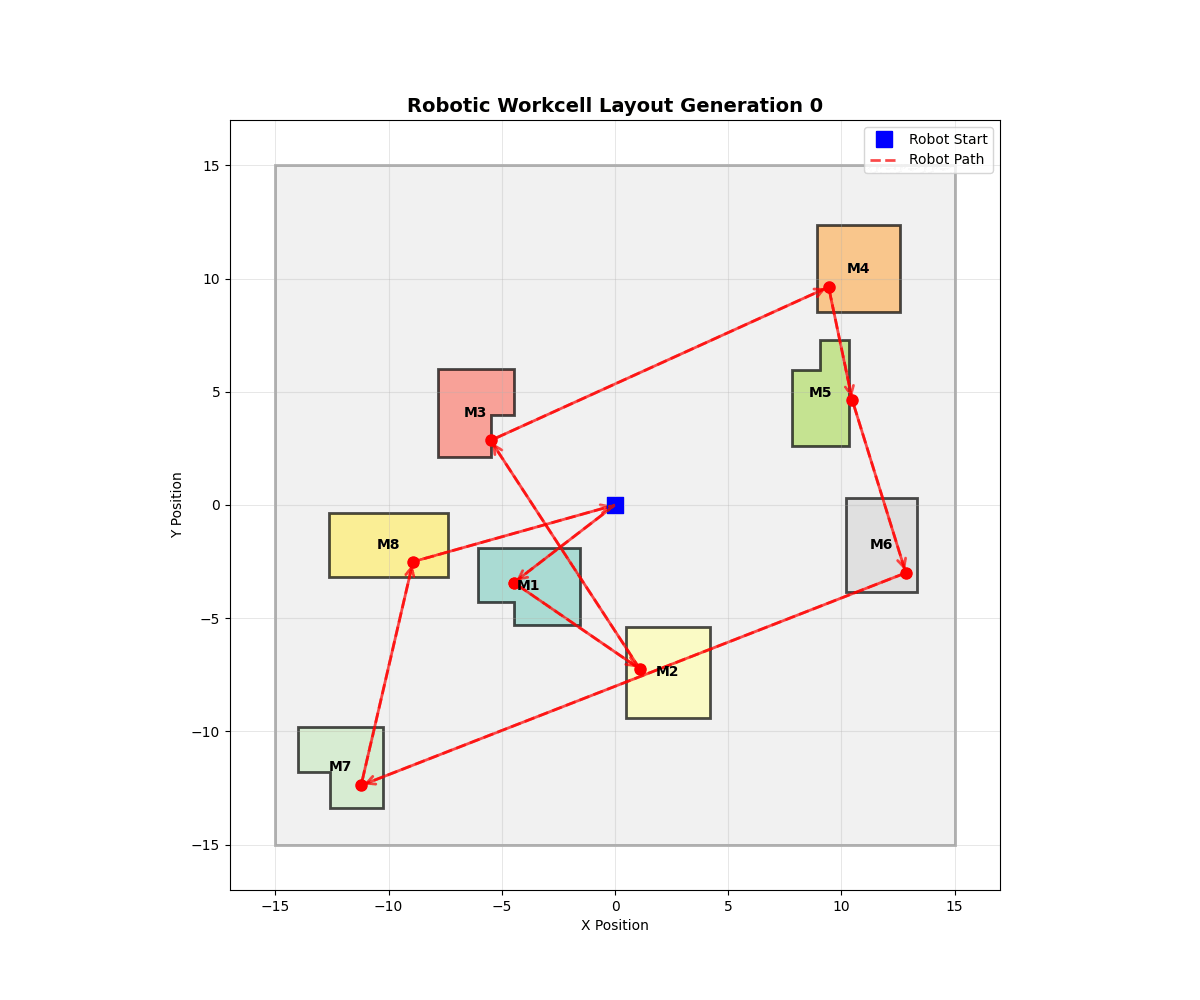
\includegraphics[width=\linewidth]{results_pure_ga_evolution/gen0.png}
        \caption{Generation 0}
    \end{subfigure}
    \hfill
    \begin{subfigure}[b]{0.45\linewidth}
        \centering
        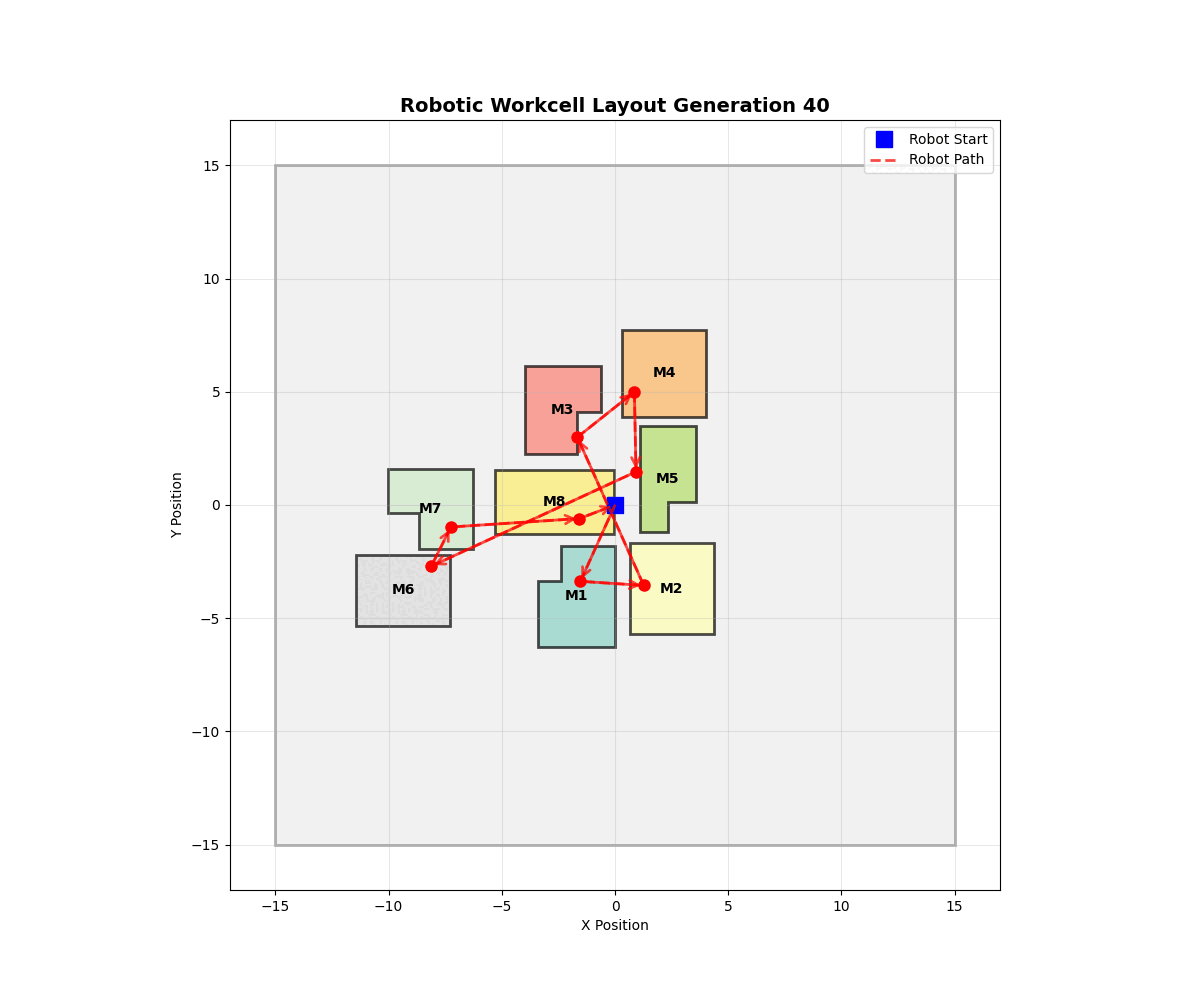
\includegraphics[width=\linewidth]{results_pure_ga_evolution/gen40.png}
        \caption{Generation 40}
    \end{subfigure}

    \vspace{0.5cm}

    \begin{subfigure}[b]{0.45\linewidth}
        \centering
        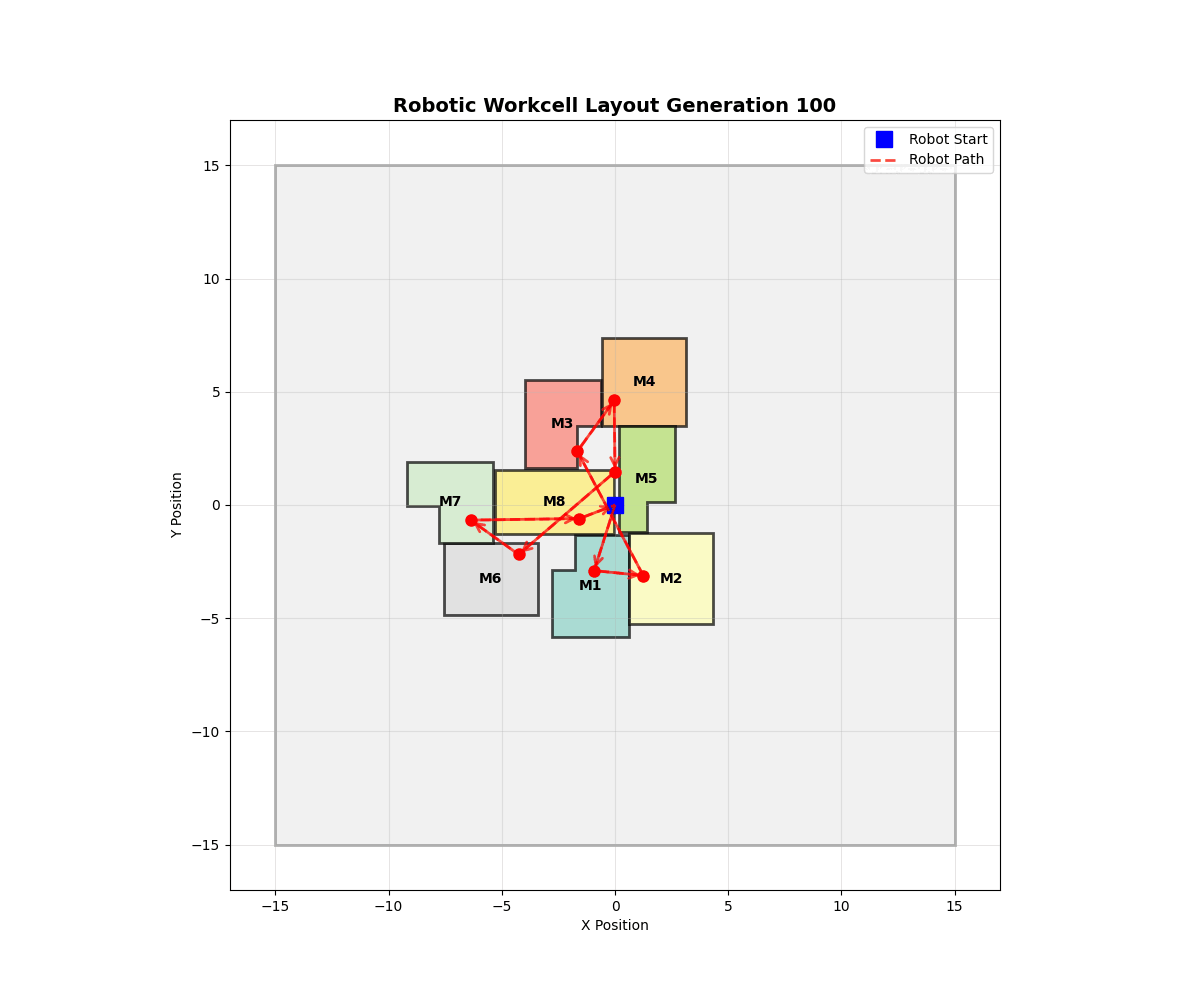
\includegraphics[width=\linewidth]{results_pure_ga_evolution/gen100.png}
        \caption{Generation 100}
    \end{subfigure}
    \hfill
    \begin{subfigure}[b]{0.45\linewidth}
        \centering
        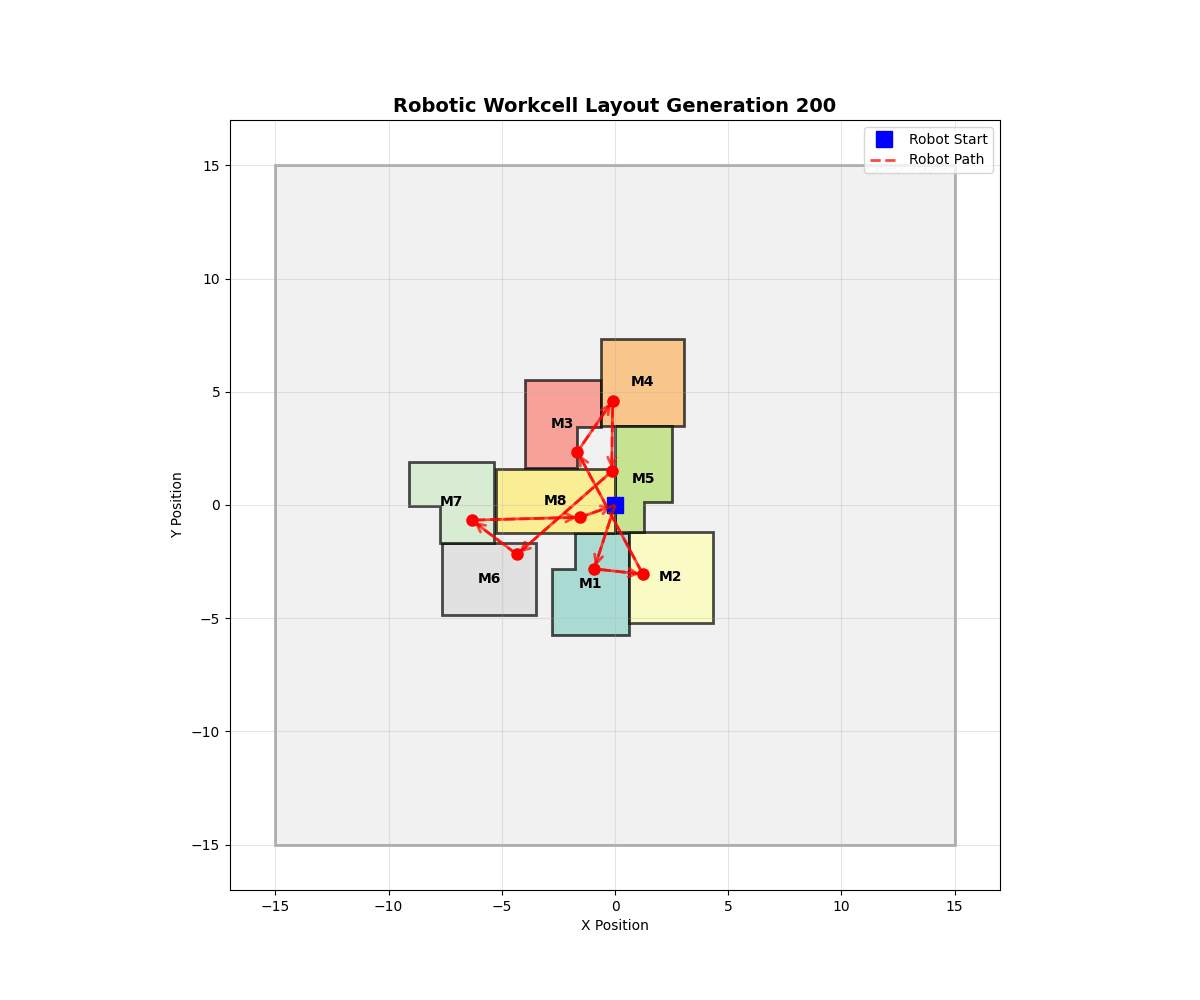
\includegraphics[width=\linewidth]{results_pure_ga_evolution/gen200.png}
        \caption{Generation 200}
    \end{subfigure}

    \caption{Evolution of the robotic workcell layout at selected generations.}
\end{figure}

%----------------------------------------
\subsection{Initial vs Final Comparison}
%----------------------------------------

\begin{figure}[H]
    \centering
    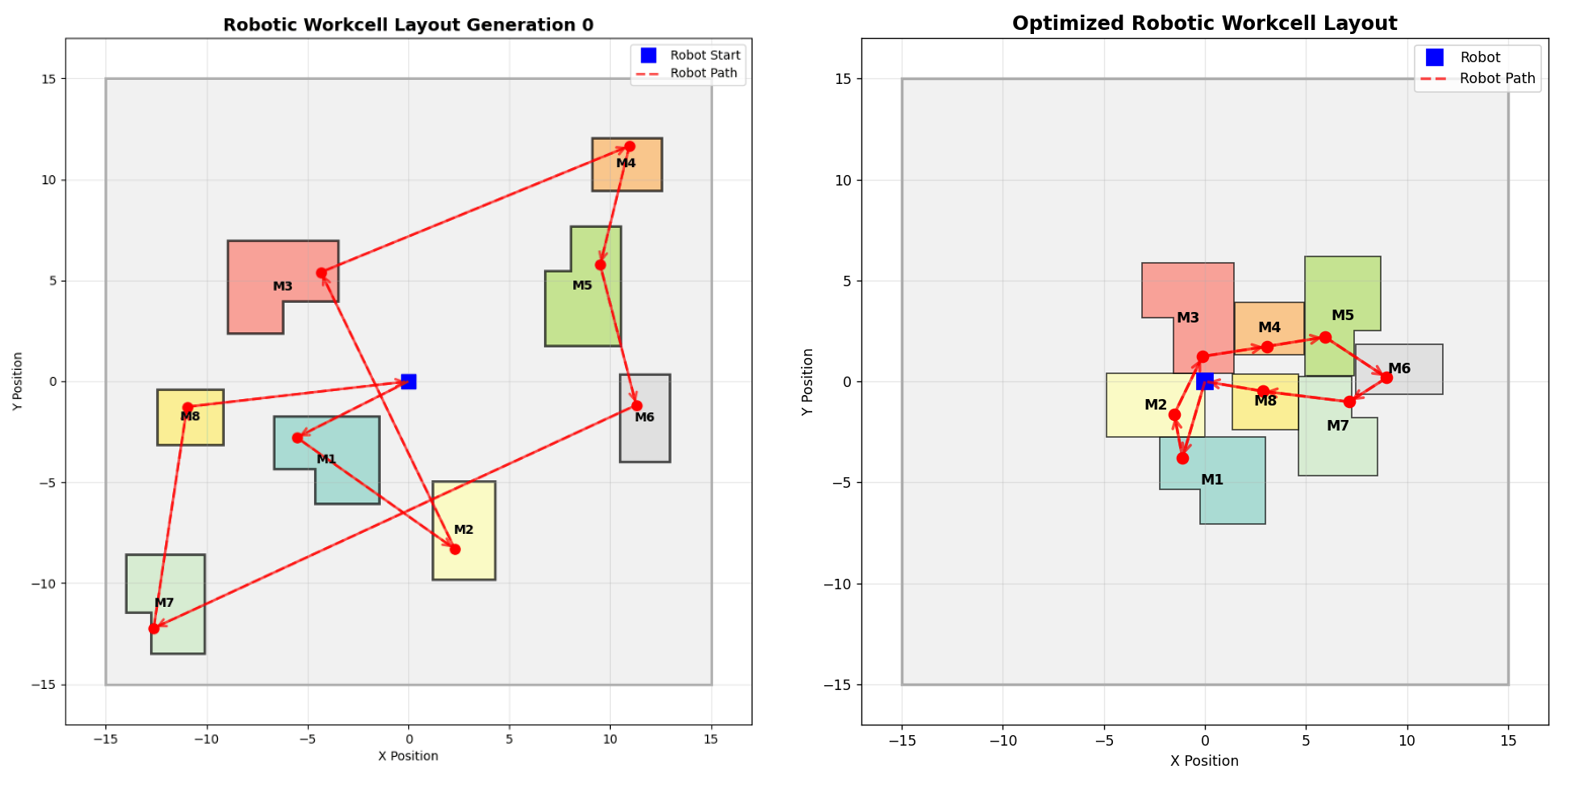
\includegraphics[width=0.8\linewidth]{results_pure_ga_evolution/comparison.png}
    \caption{Comparison between initial and final optimized layouts.}
\end{figure}

\section{Appendix: GA Grid Search Figures}
%====================================================
\subsection{Population Size = 100}
%====================================================

\subsubsection{Generations = 100}
\begin{figure}[H]
    \centering
    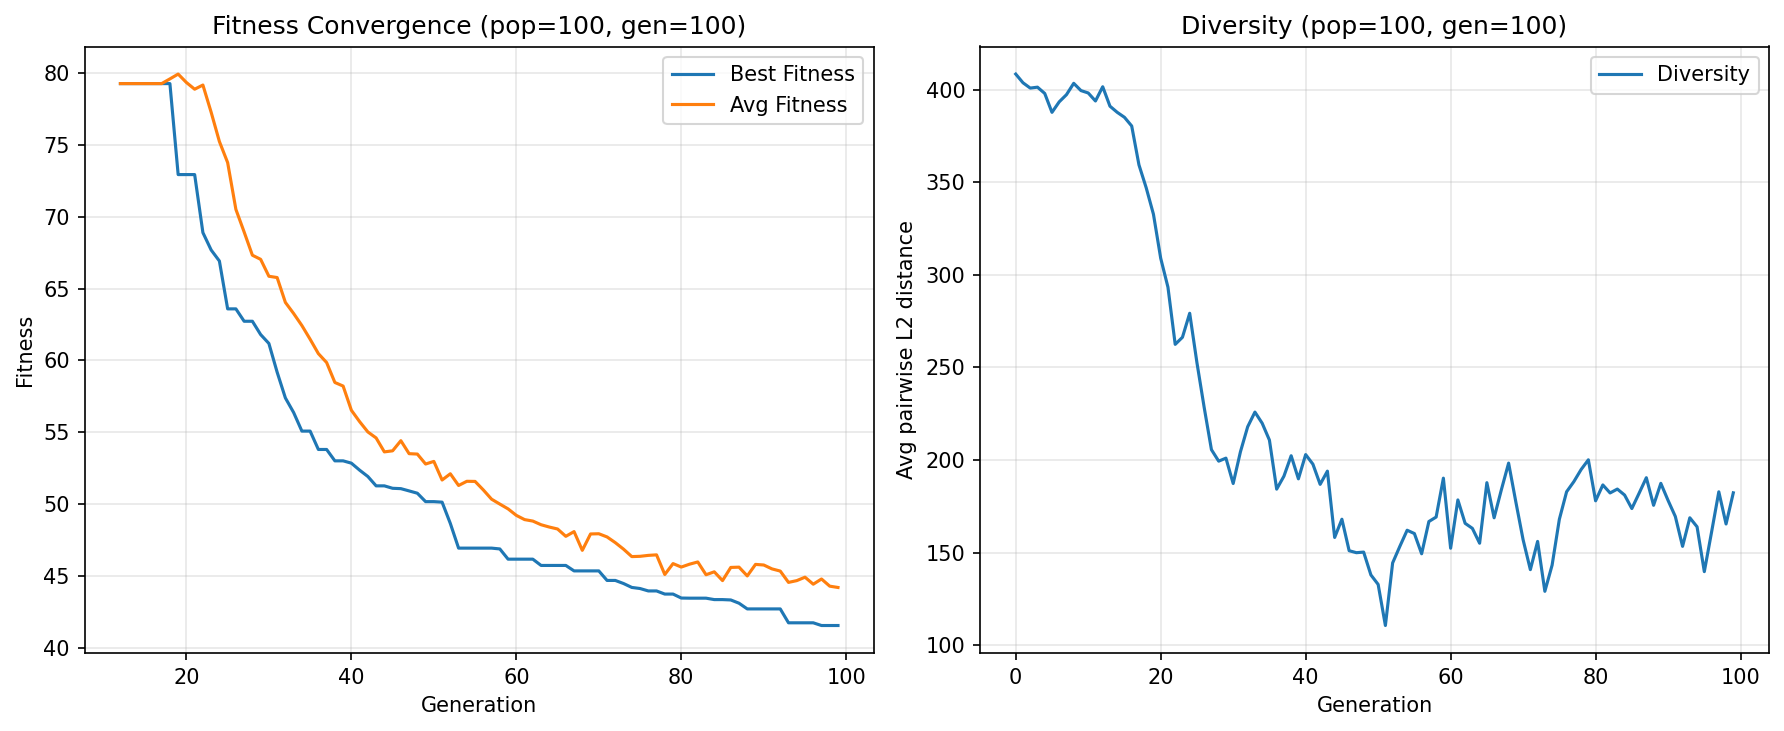
\includegraphics[width=0.9\linewidth]{ga_grid_results_incremental/pop_100/pop_100_gen_100.png}
    \caption{Fitness convergence and diversity plot for population size 100 and 100 generations.}
\end{figure}

\begin{figure}[H]
    \centering
    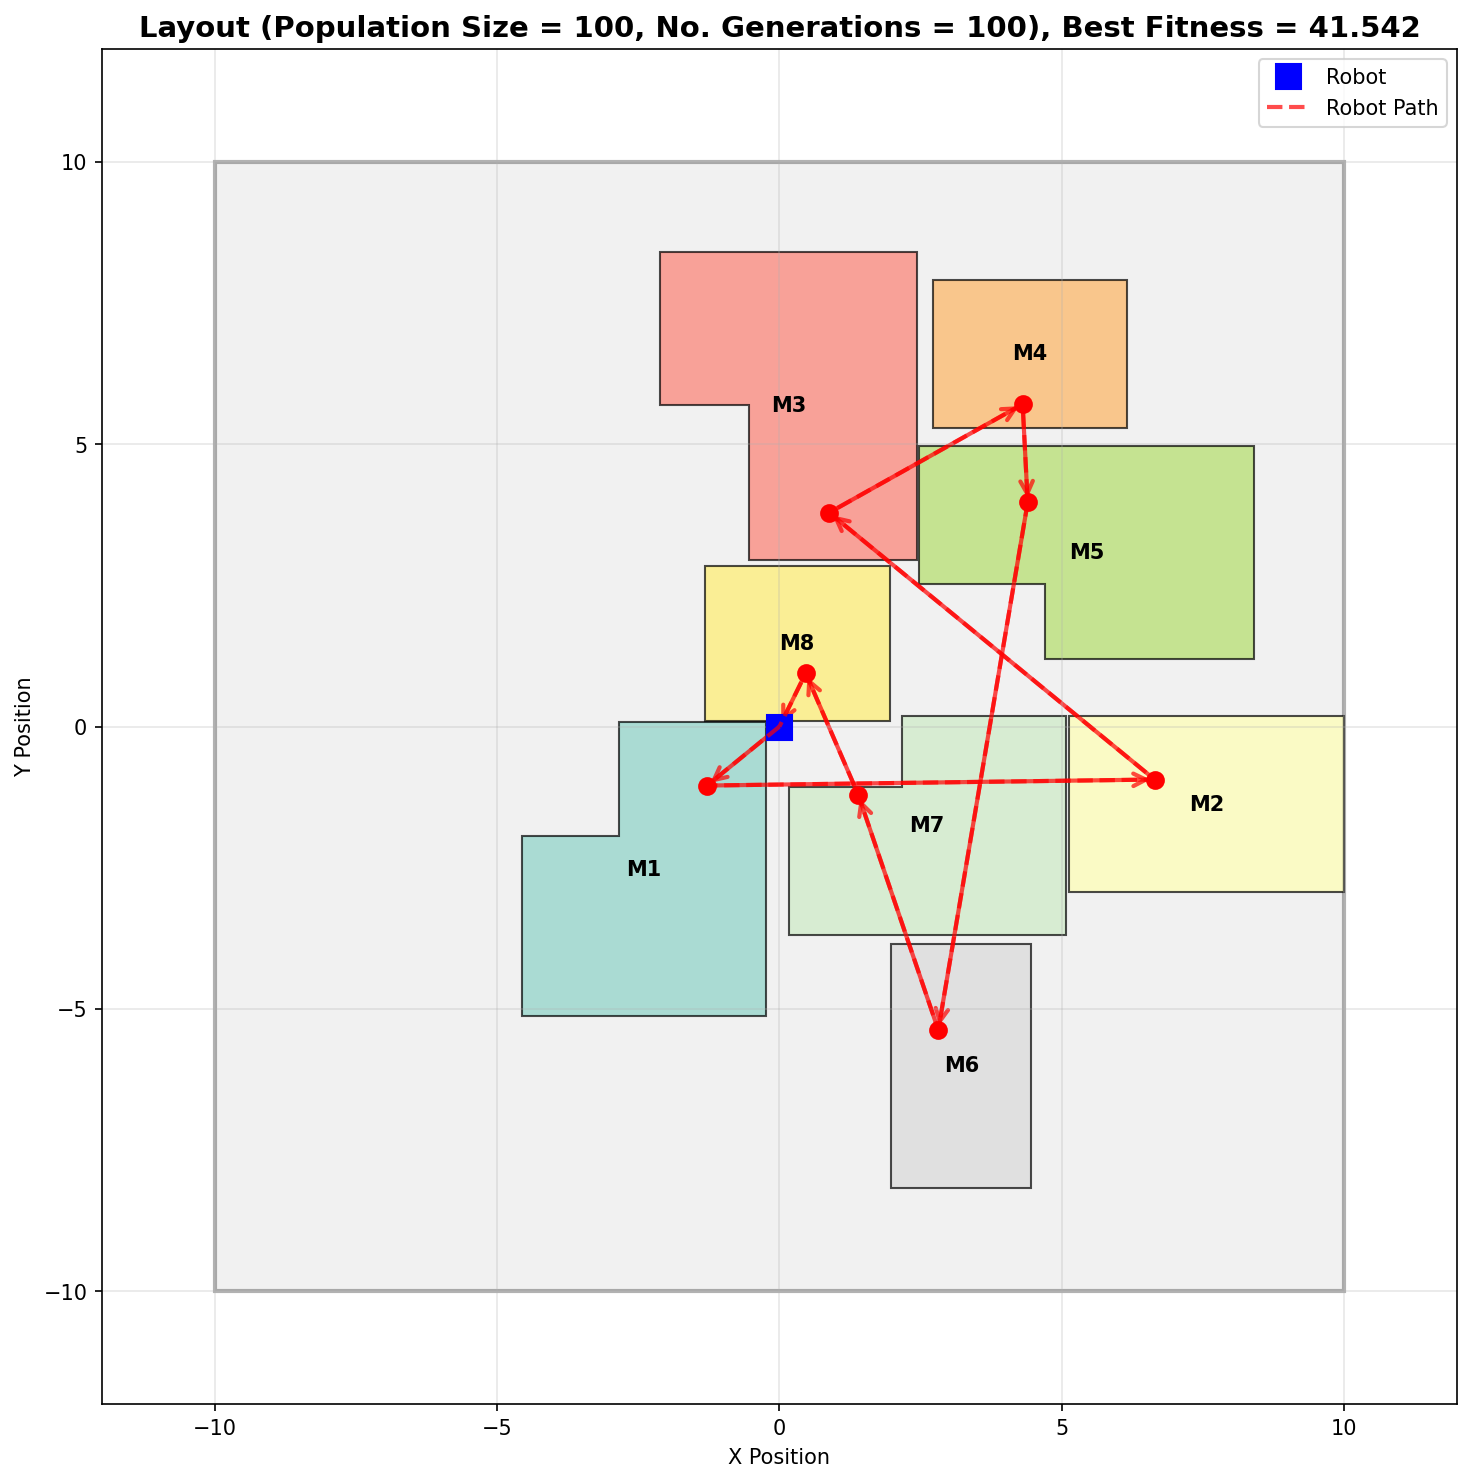
\includegraphics[width=0.7\linewidth]{ga_grid_results_incremental/pop_100/layout_pop_100_gen_100.png}
    \caption{Final optimized layout for population size 100 and 100 generations.}
\end{figure}

\clearpage

\subsubsection{Generations = 200}
\begin{figure}[H]
    \centering
    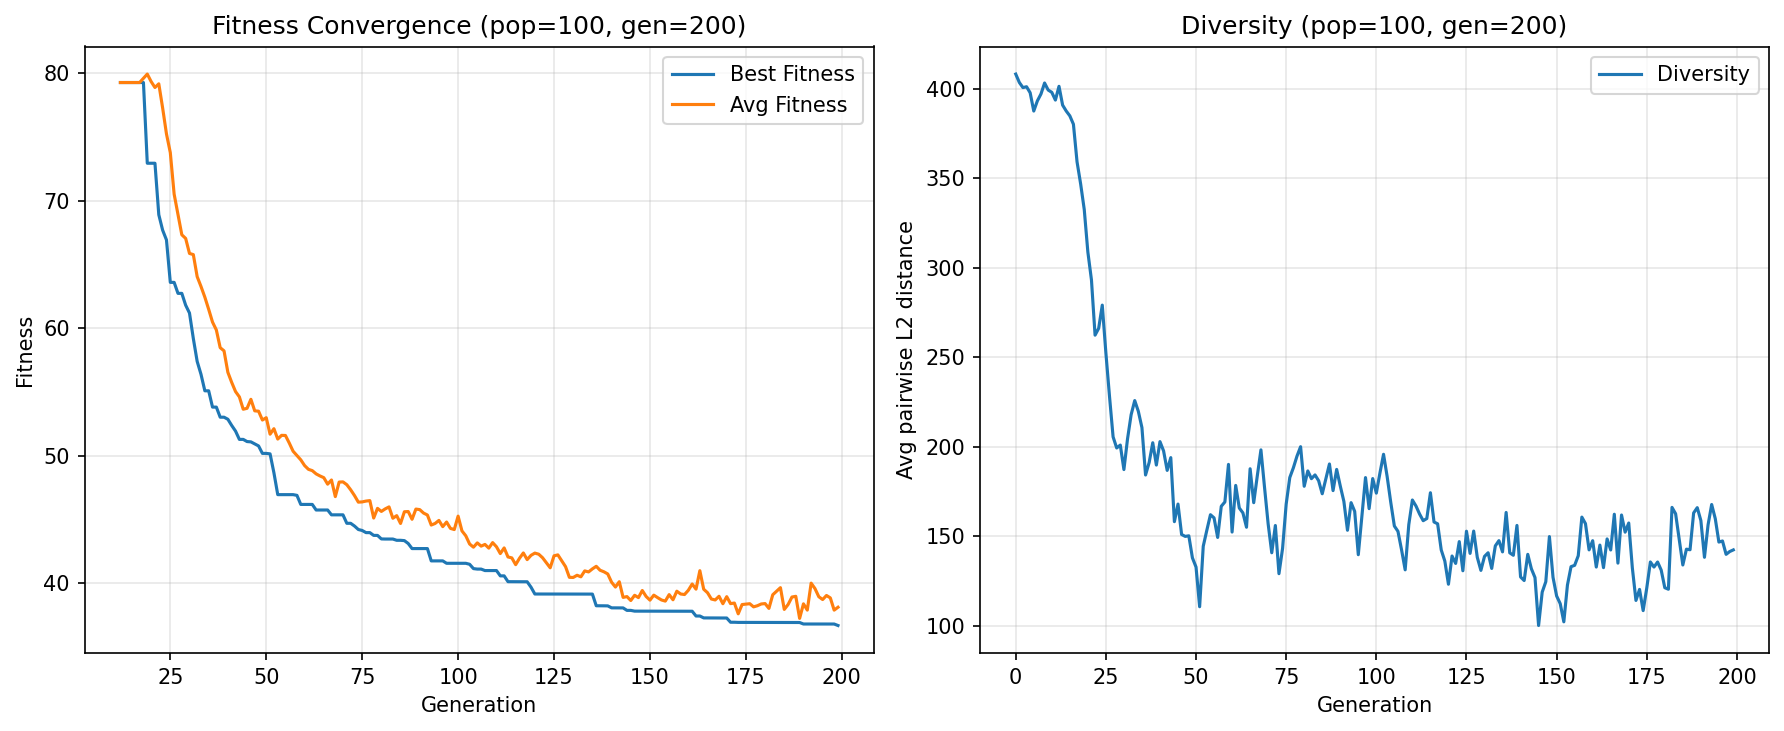
\includegraphics[width=0.9\linewidth]{ga_grid_results_incremental/pop_100/pop_100_gen_200.png}
    \caption{Fitness convergence and diversity plot for population size 100 and 200 generations.}
\end{figure}

\begin{figure}[H]
    \centering
    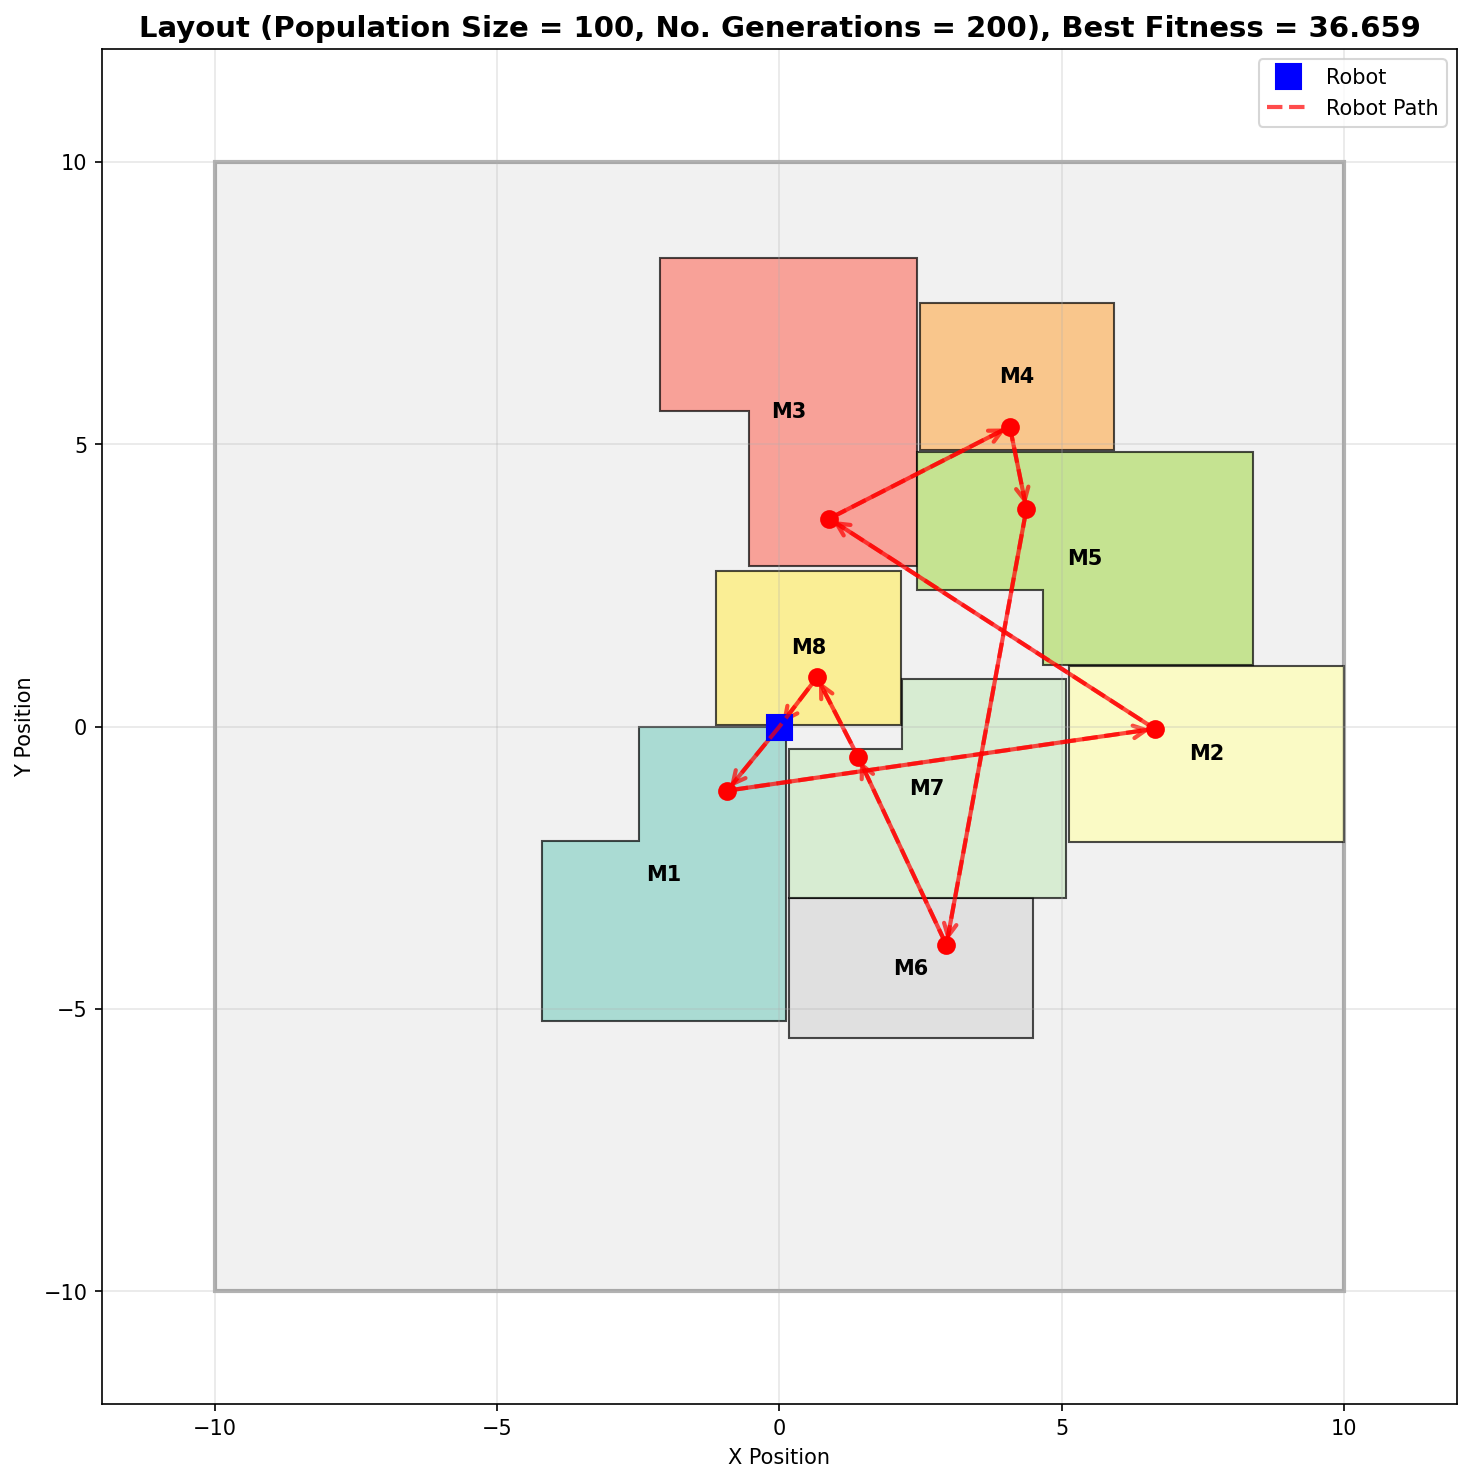
\includegraphics[width=0.7\linewidth]{ga_grid_results_incremental/pop_100/layout_pop_100_gen_200.png}
    \caption{Final optimized layout for population size 100 and 200 generations.}
\end{figure}

\clearpage

\subsubsection{Generations = 500}
\begin{figure}[H]
    \centering
    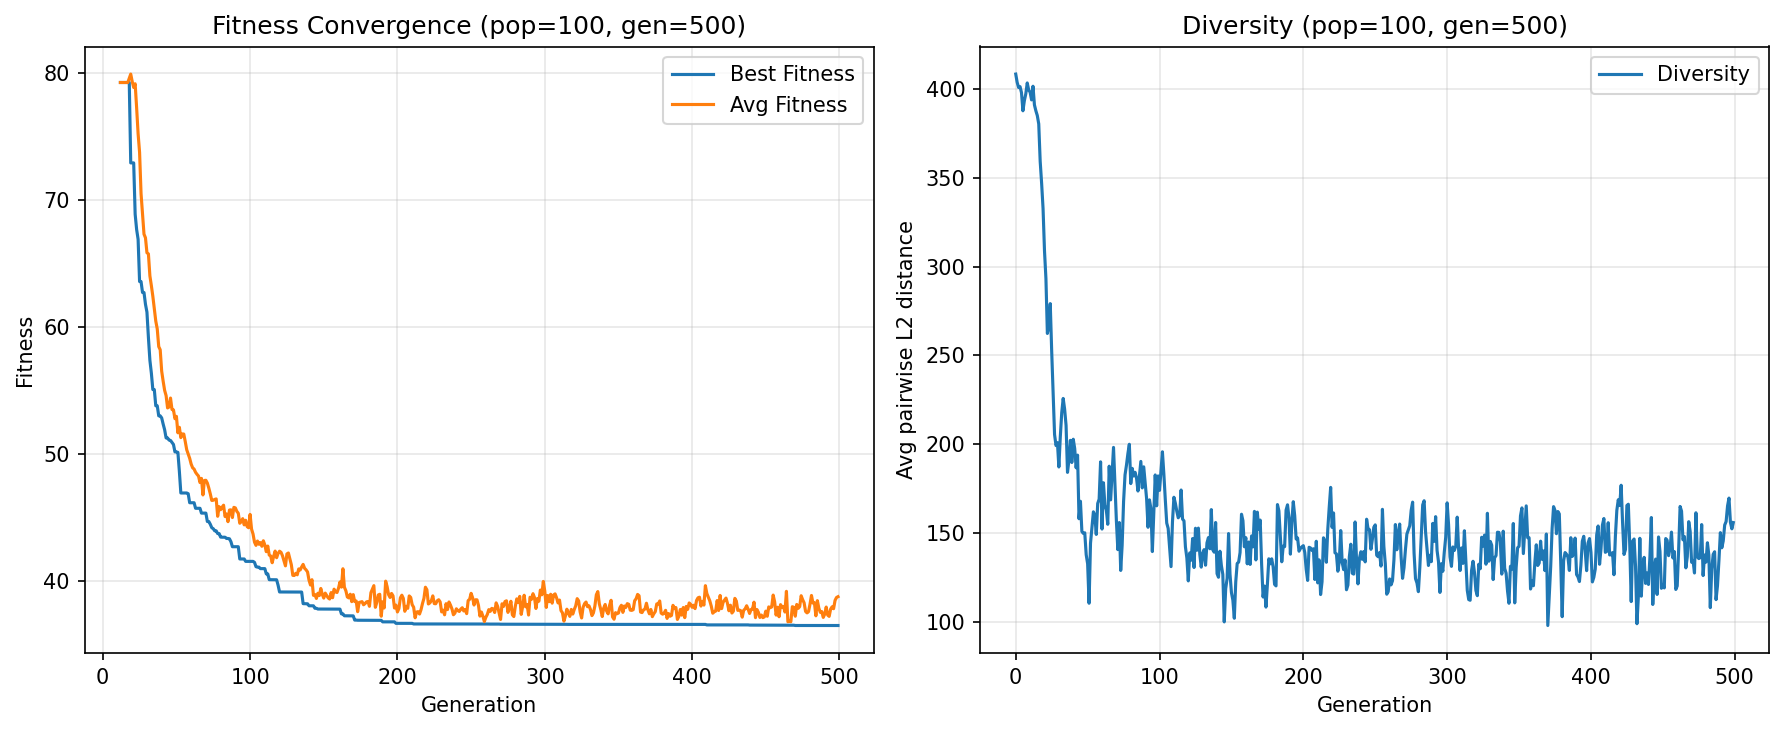
\includegraphics[width=0.9\linewidth]{ga_grid_results_incremental/pop_100/pop_100_gen_500.png}
    \caption{Fitness convergence and diversity plot for population size 100 and 500 generations.}
\end{figure}

\begin{figure}[H]
    \centering
    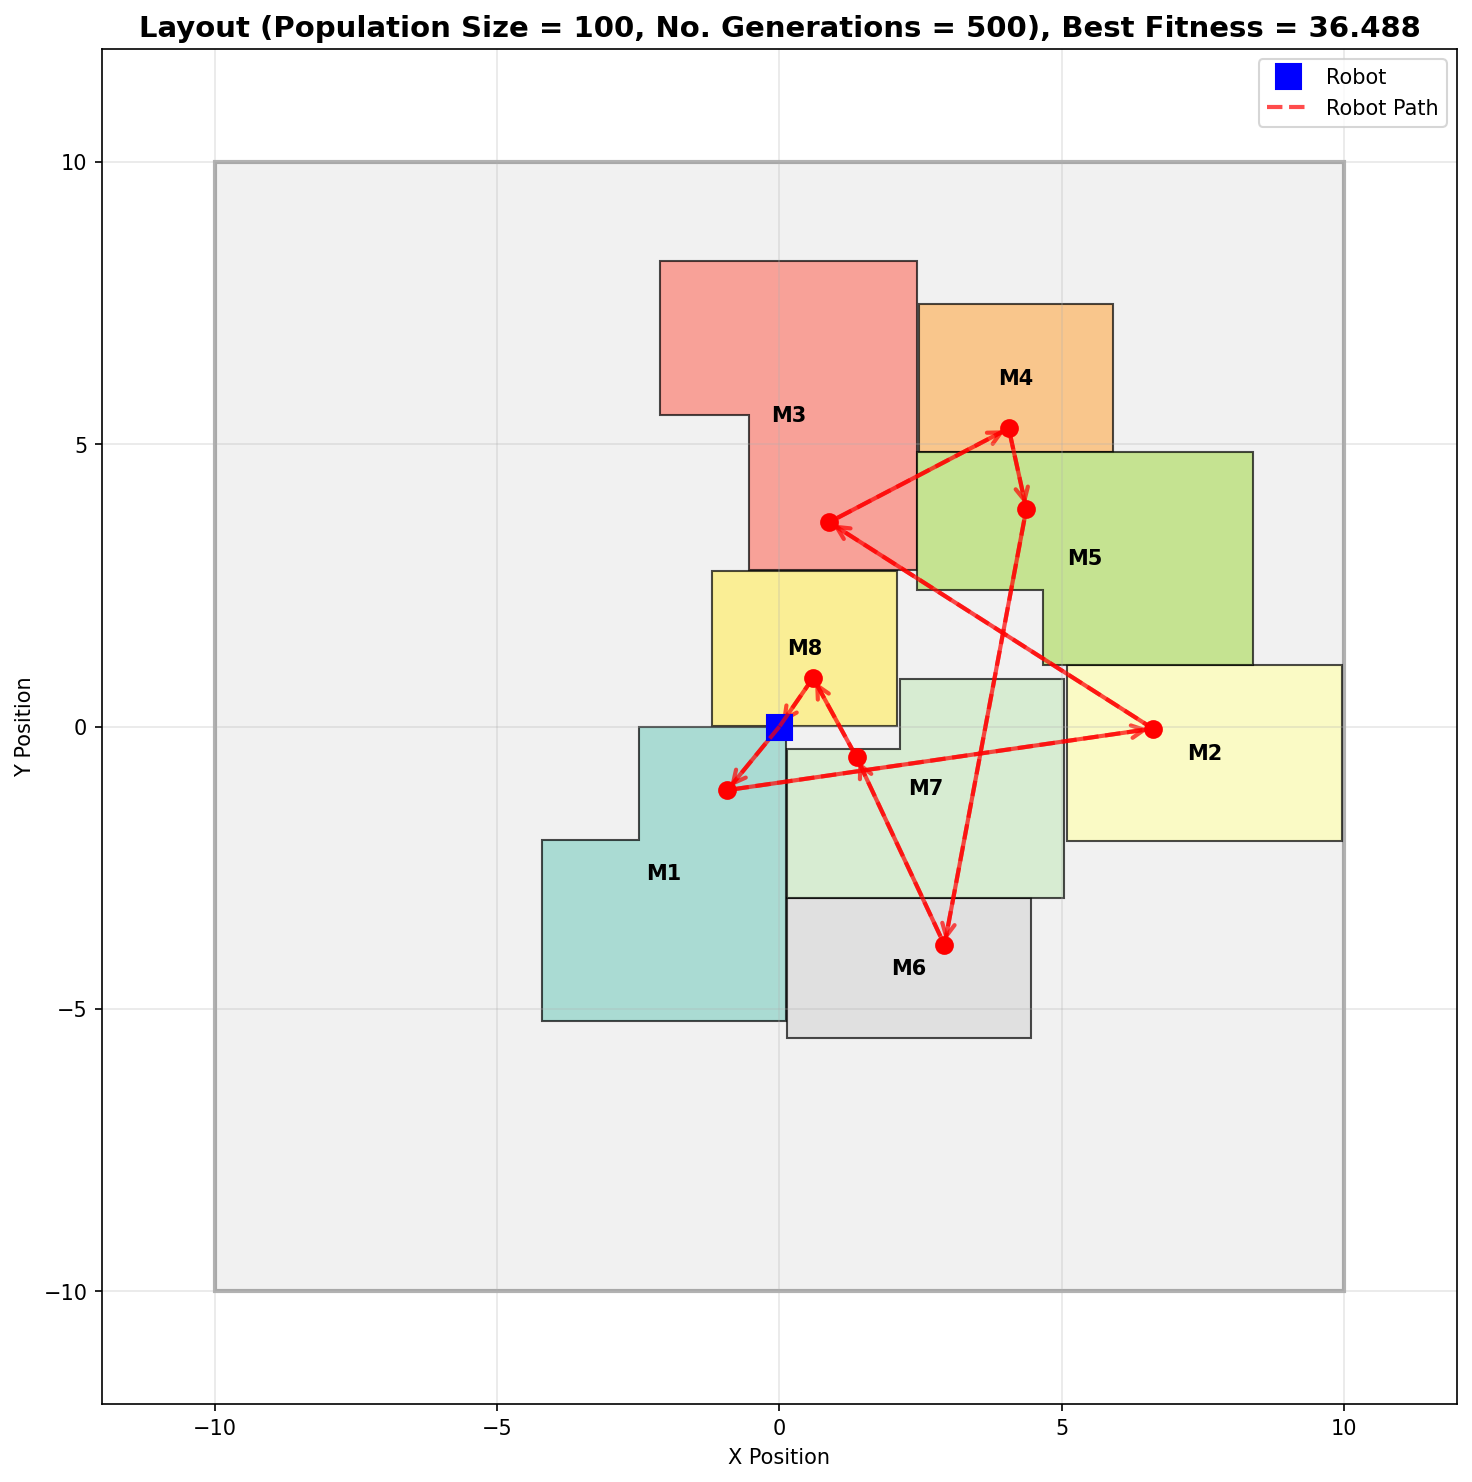
\includegraphics[width=0.7\linewidth]{ga_grid_results_incremental/pop_100/layout_pop_100_gen_500.png}
    \caption{Final optimized layout for population size 100 and 500 generations.}
\end{figure}

\clearpage

\subsubsection{Generations = 1000}
\begin{figure}[H]
    \centering
    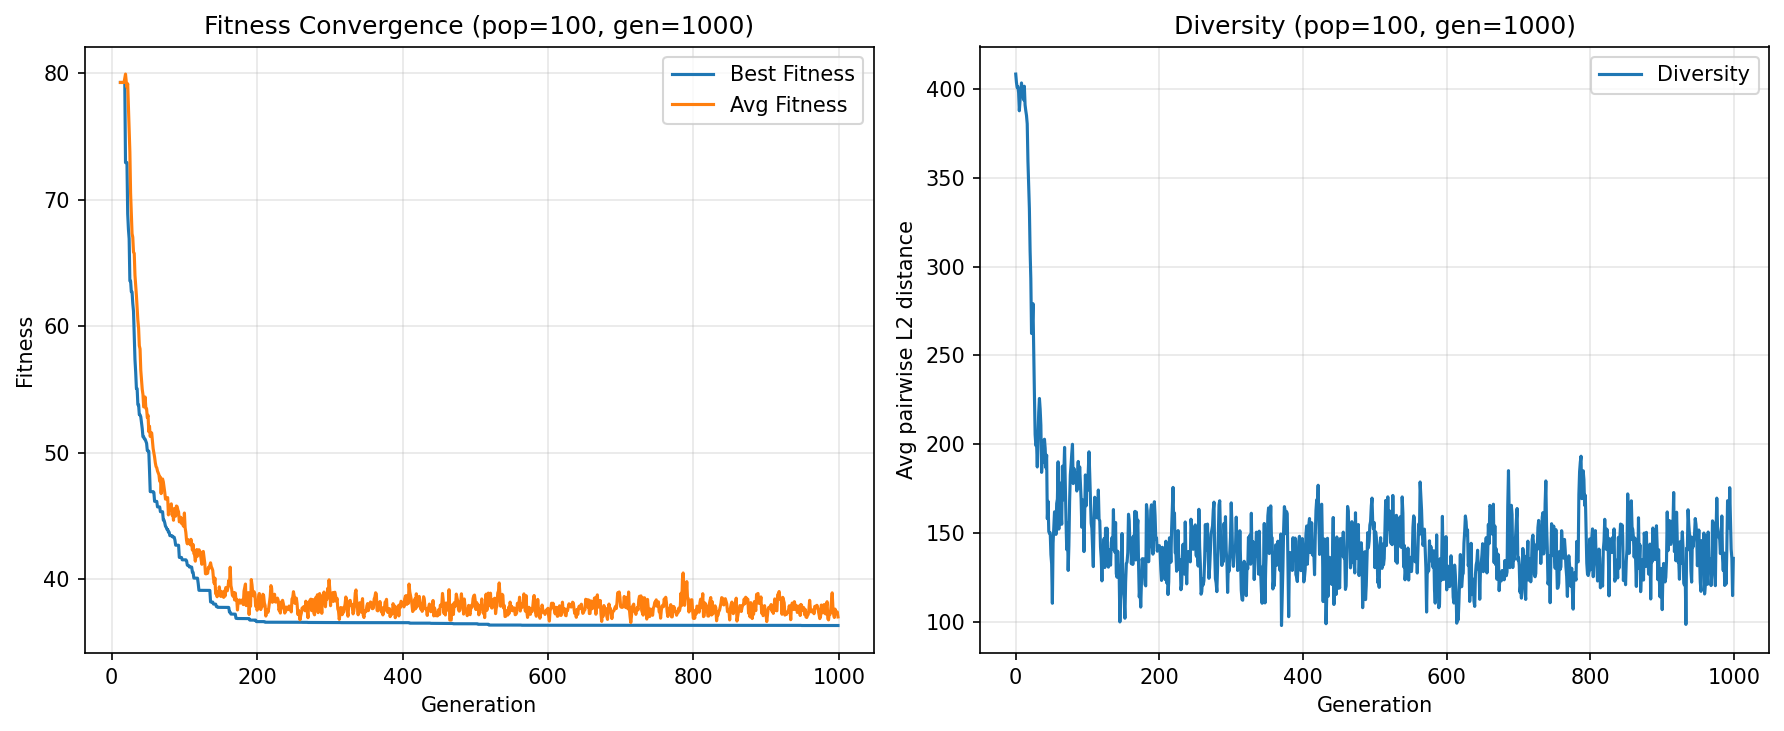
\includegraphics[width=0.9\linewidth]{ga_grid_results_incremental/pop_100/pop_100_gen_1000.png}
    \caption{Fitness convergence and diversity plot for population size 100 and 1000 generations.}
\end{figure}

\begin{figure}[H]
    \centering
    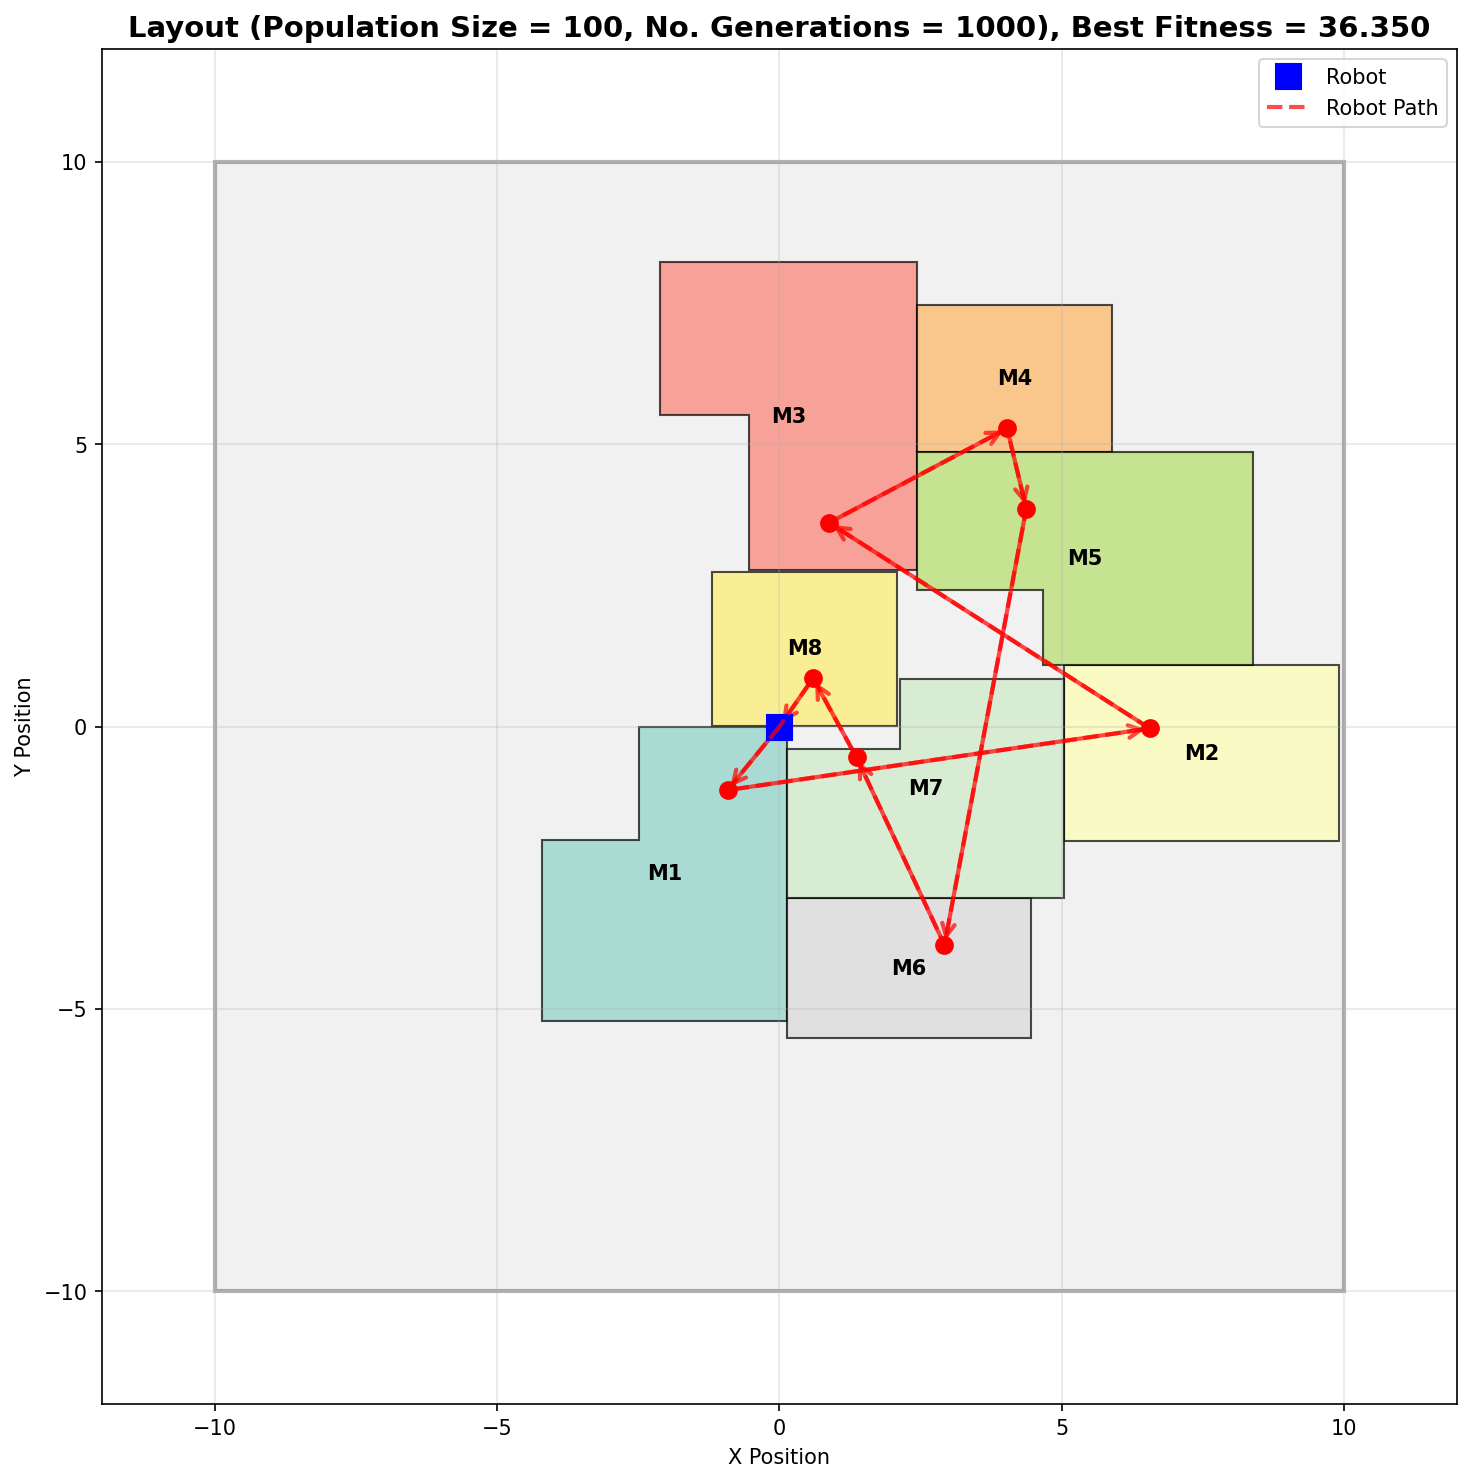
\includegraphics[width=0.7\linewidth]{ga_grid_results_incremental/pop_100/layout_pop_100_gen_1000.png}
    \caption{Final optimized layout for population size 100 and 1000 generations.}
\end{figure}

\clearpage

\subsubsection{Generations = 2000}
\begin{figure}[H]
    \centering
    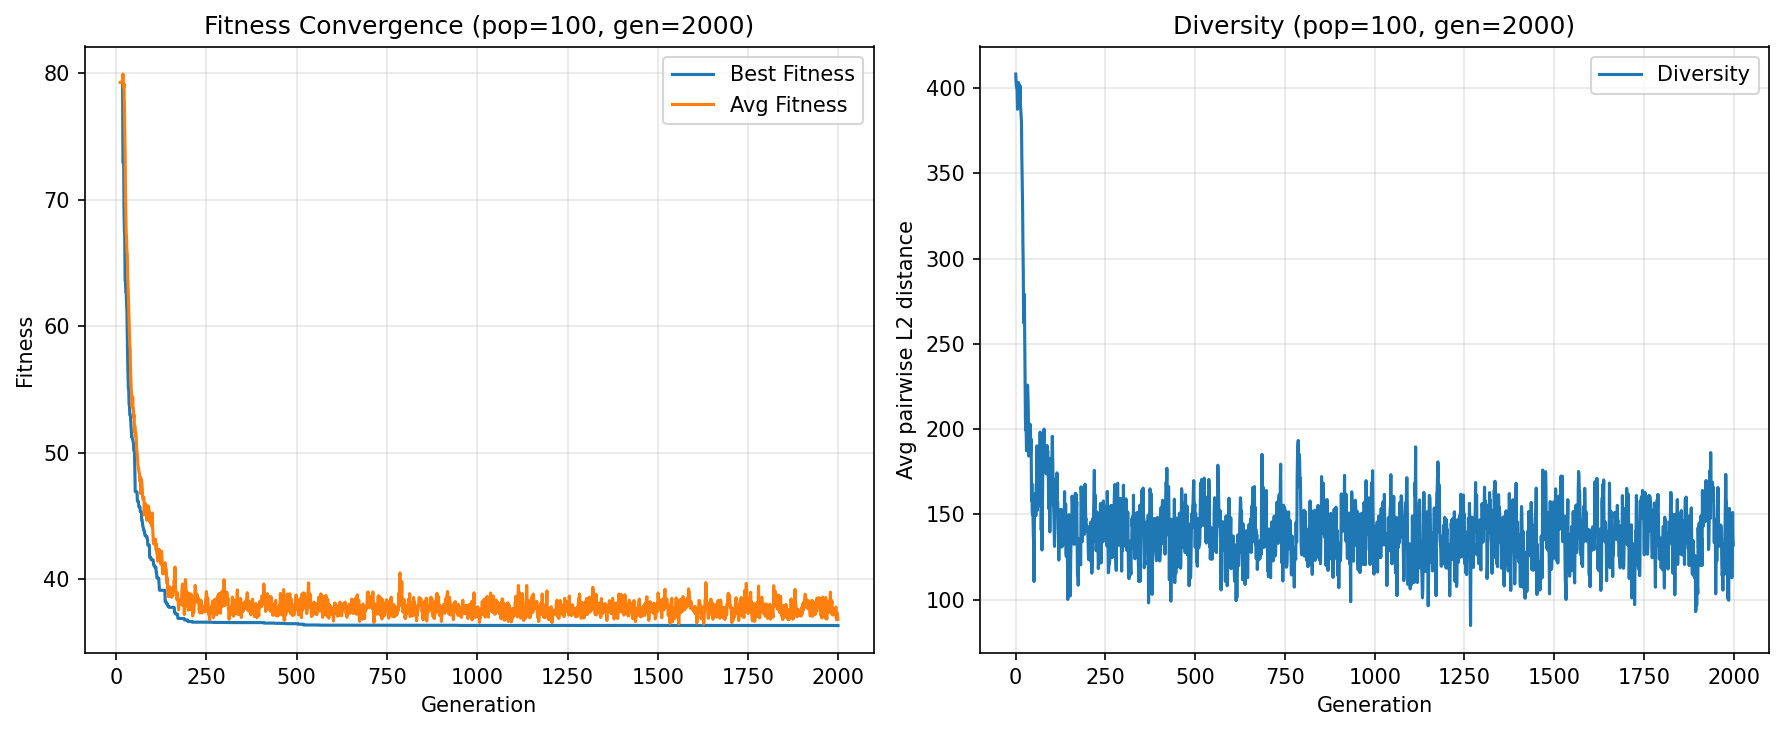
\includegraphics[width=0.9\linewidth]{ga_grid_results_incremental/pop_100/pop_100_gen_2000.png}
    \caption{Fitness convergence and diversity plot for population size 100 and 2000 generations.}
\end{figure}

\begin{figure}[H]
    \centering
    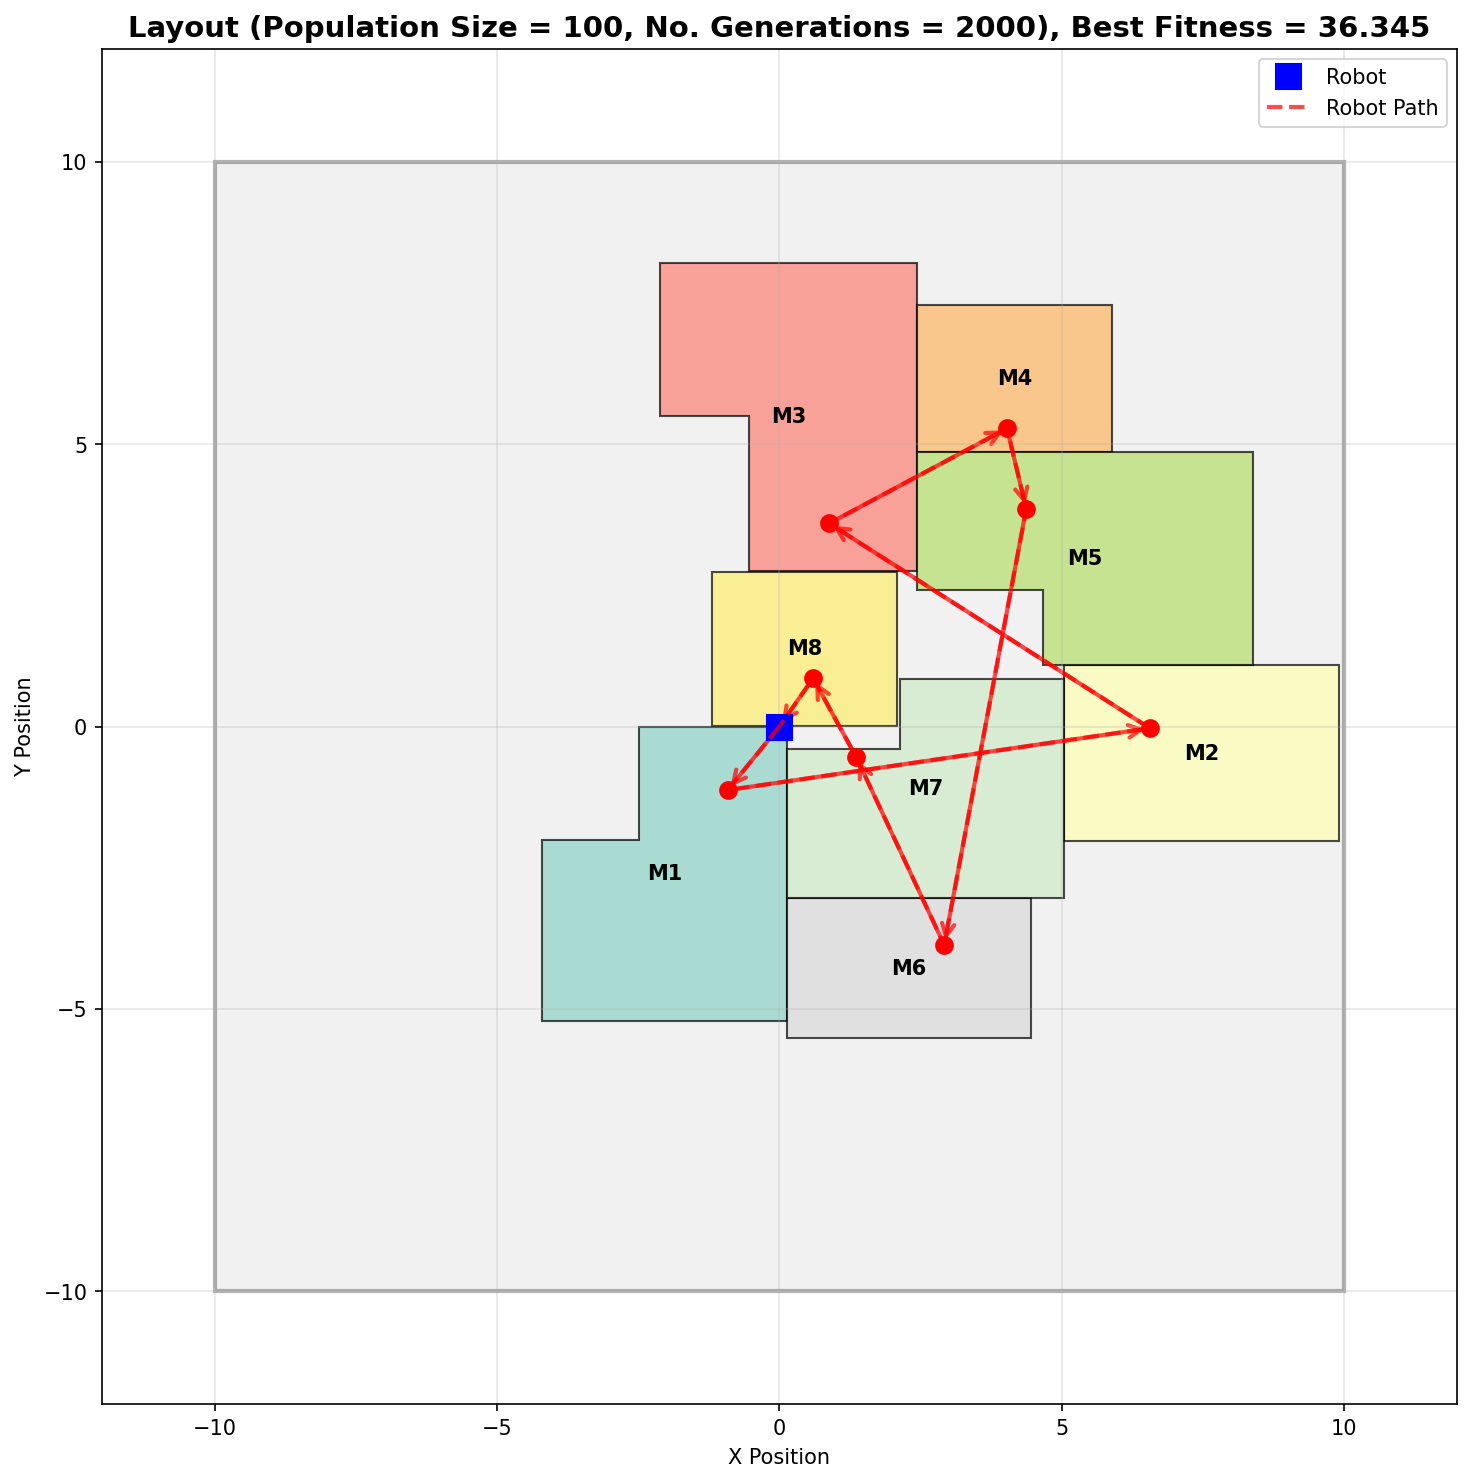
\includegraphics[width=0.7\linewidth]{ga_grid_results_incremental/pop_100/layout_pop_100_gen_2000.png}
    \caption{Final optimized layout for population size 100 and 2000 generations.}
\end{figure}

\clearpage

%====================================================
\subsection{Population Size = 200}
%====================================================

\subsubsection{Generations = 100}
\begin{figure}[H]
    \centering
    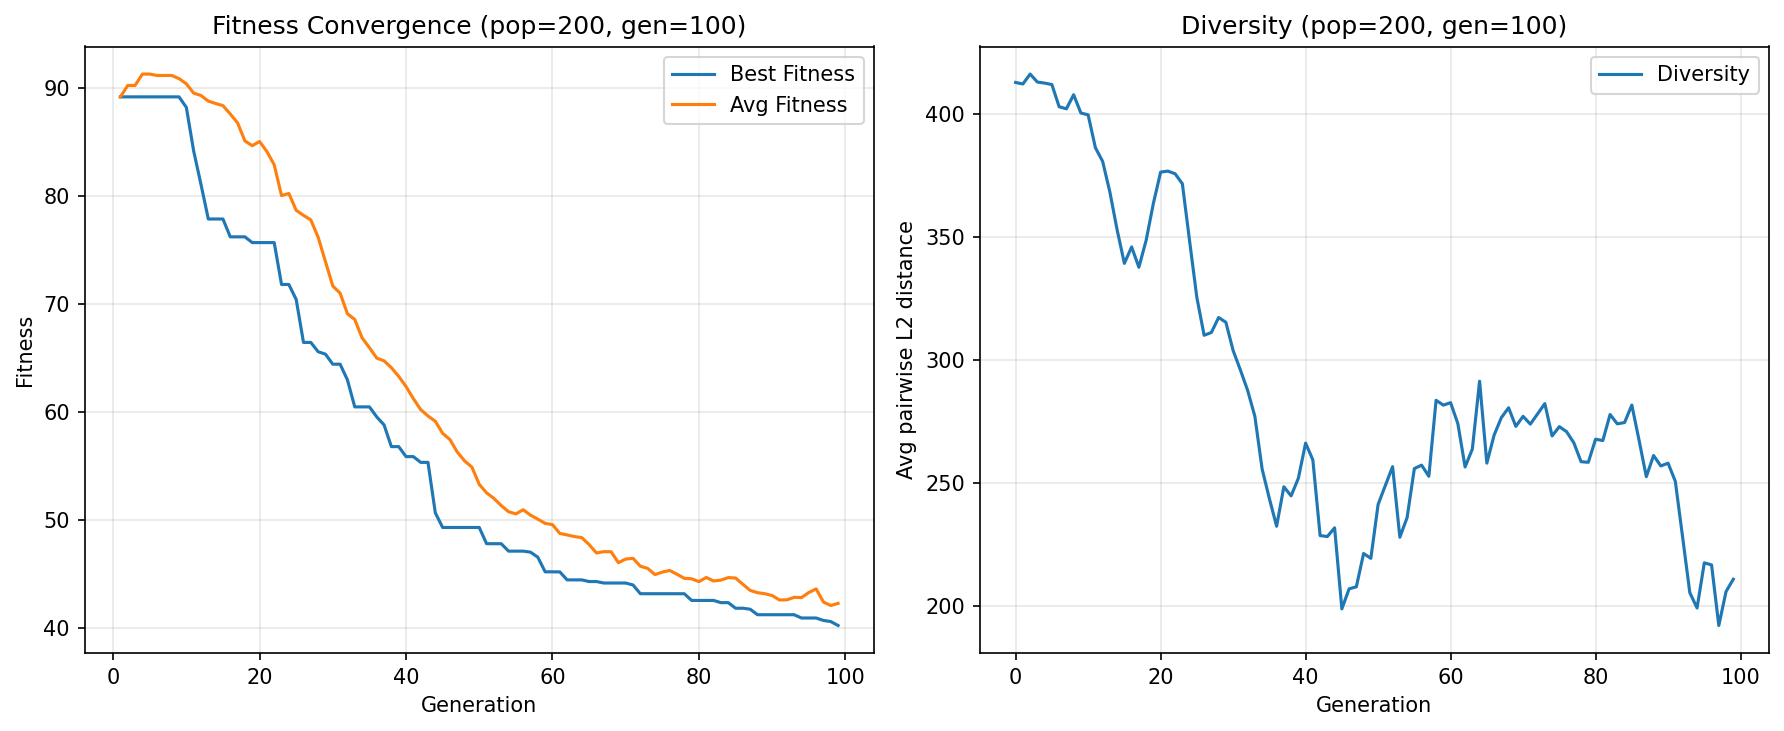
\includegraphics[width=0.9\linewidth]{ga_grid_results_incremental/pop_200/pop_200_gen_100.png}
    \caption{Fitness convergence and diversity plot for population size 200 and 100 generations.}
\end{figure}

\begin{figure}[H]
    \centering
    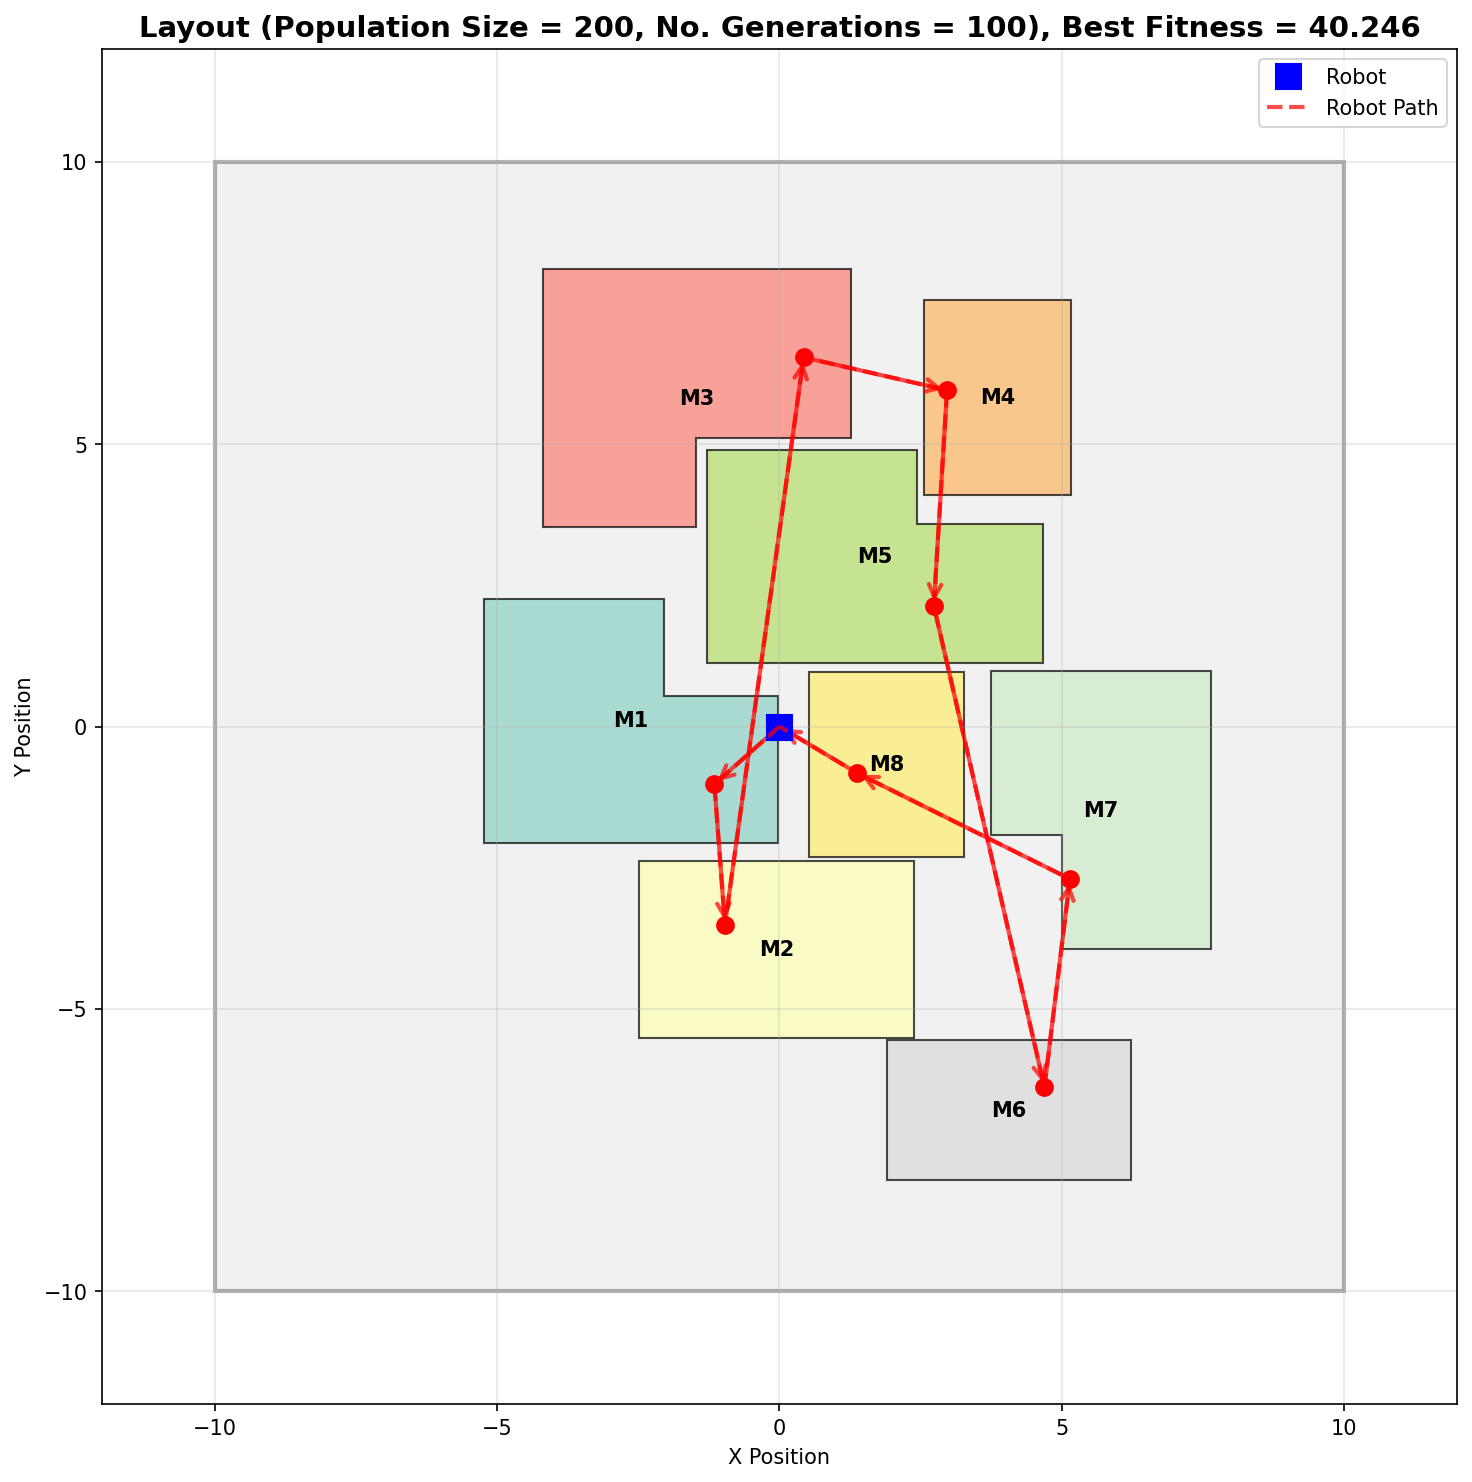
\includegraphics[width=0.7\linewidth]{ga_grid_results_incremental/pop_200/layout_pop_200_gen_100.png}
    \caption{Final optimized layout for population size 200 and 100 generations.}
\end{figure}

\clearpage

\subsubsection{Generations = 200}
\begin{figure}[H]
    \centering
    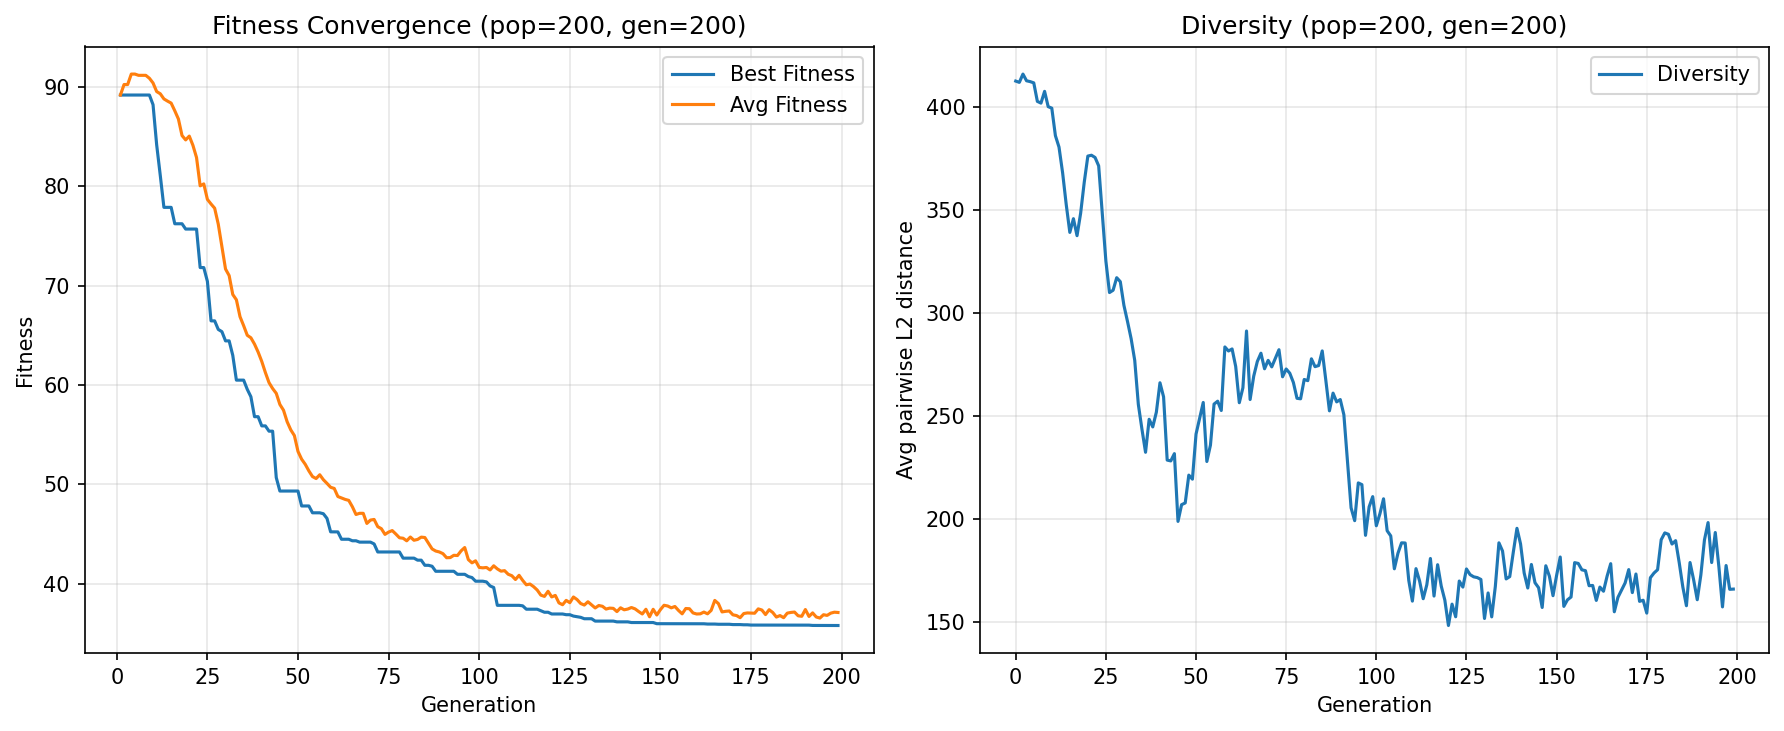
\includegraphics[width=0.9\linewidth]{ga_grid_results_incremental/pop_200/pop_200_gen_200.png}
    \caption{Fitness convergence and diversity plot for population size 200 and 200 generations.}
\end{figure}

\begin{figure}[H]
    \centering
    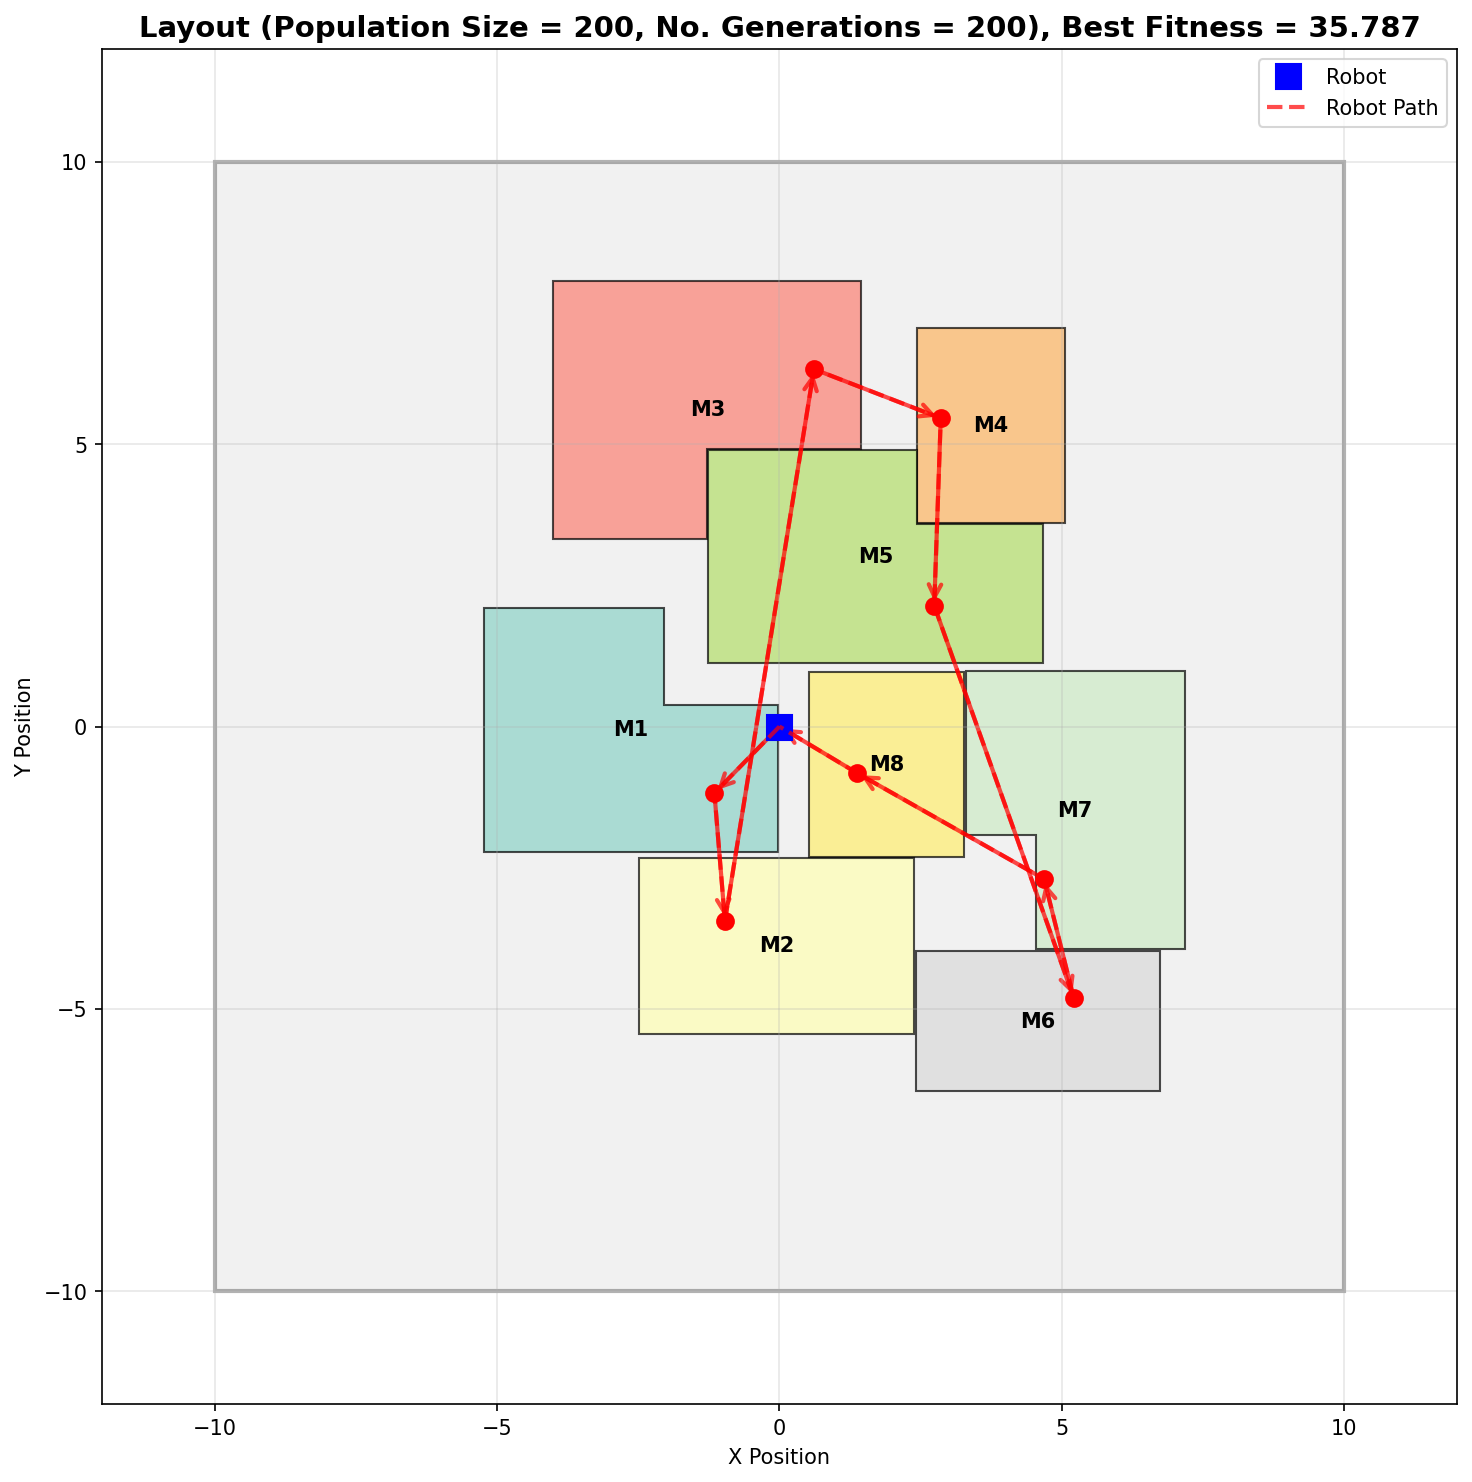
\includegraphics[width=0.7\linewidth]{ga_grid_results_incremental/pop_200/layout_pop_200_gen_200.png}
    \caption{Final optimized layout for population size 200 and 200 generations.}
\end{figure}

\clearpage

\subsubsection{Generations = 500}
\begin{figure}[H]
    \centering
    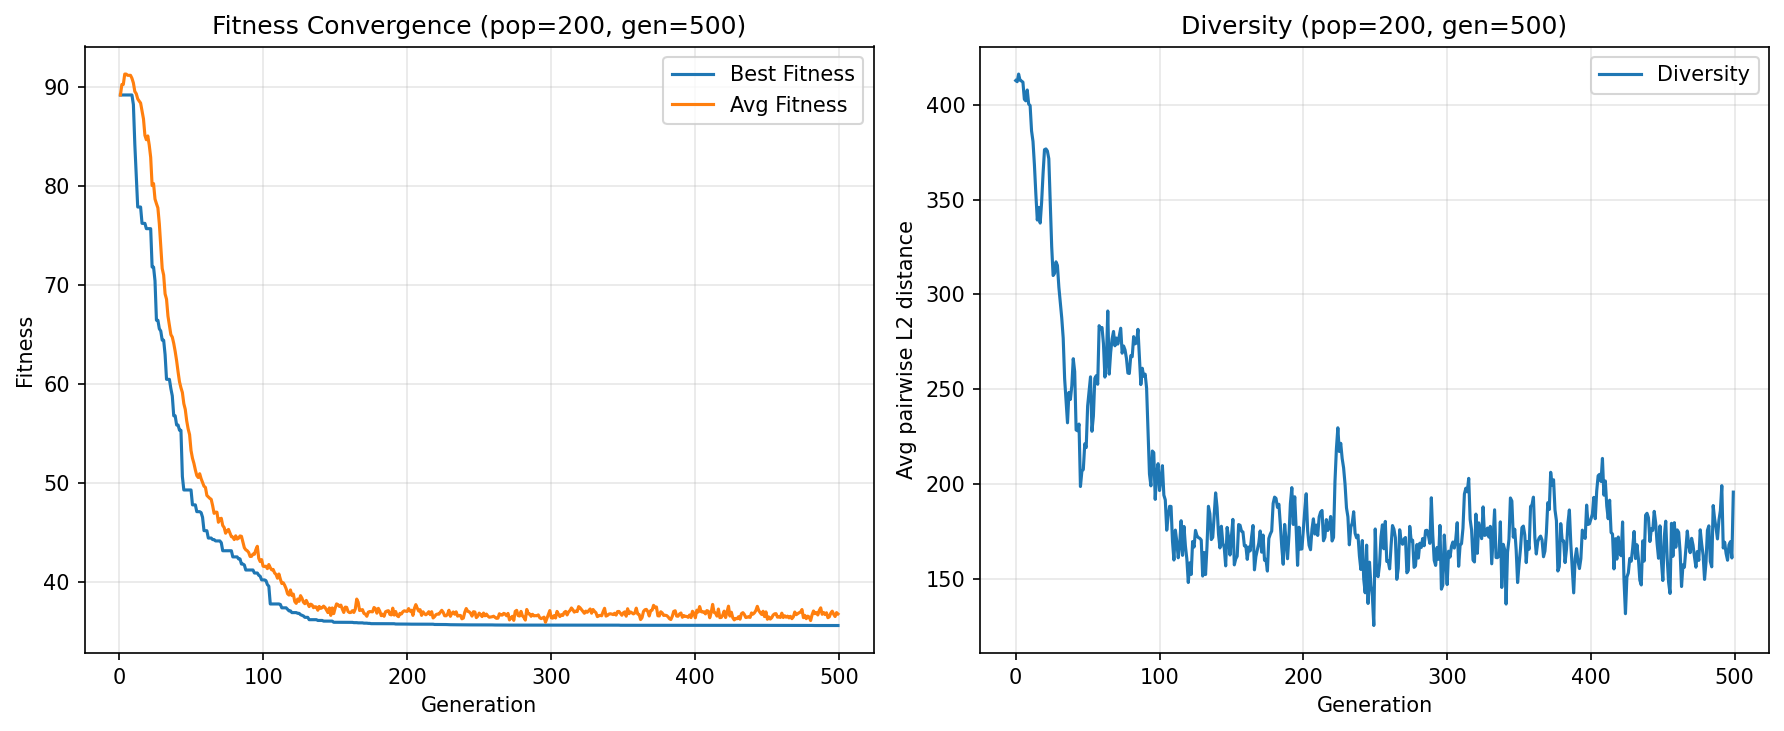
\includegraphics[width=0.9\linewidth]{ga_grid_results_incremental/pop_200/pop_200_gen_500.png}
    \caption{Fitness convergence and diversity plot for population size 200 and 500 generations.}
\end{figure}

\begin{figure}[H]
    \centering
    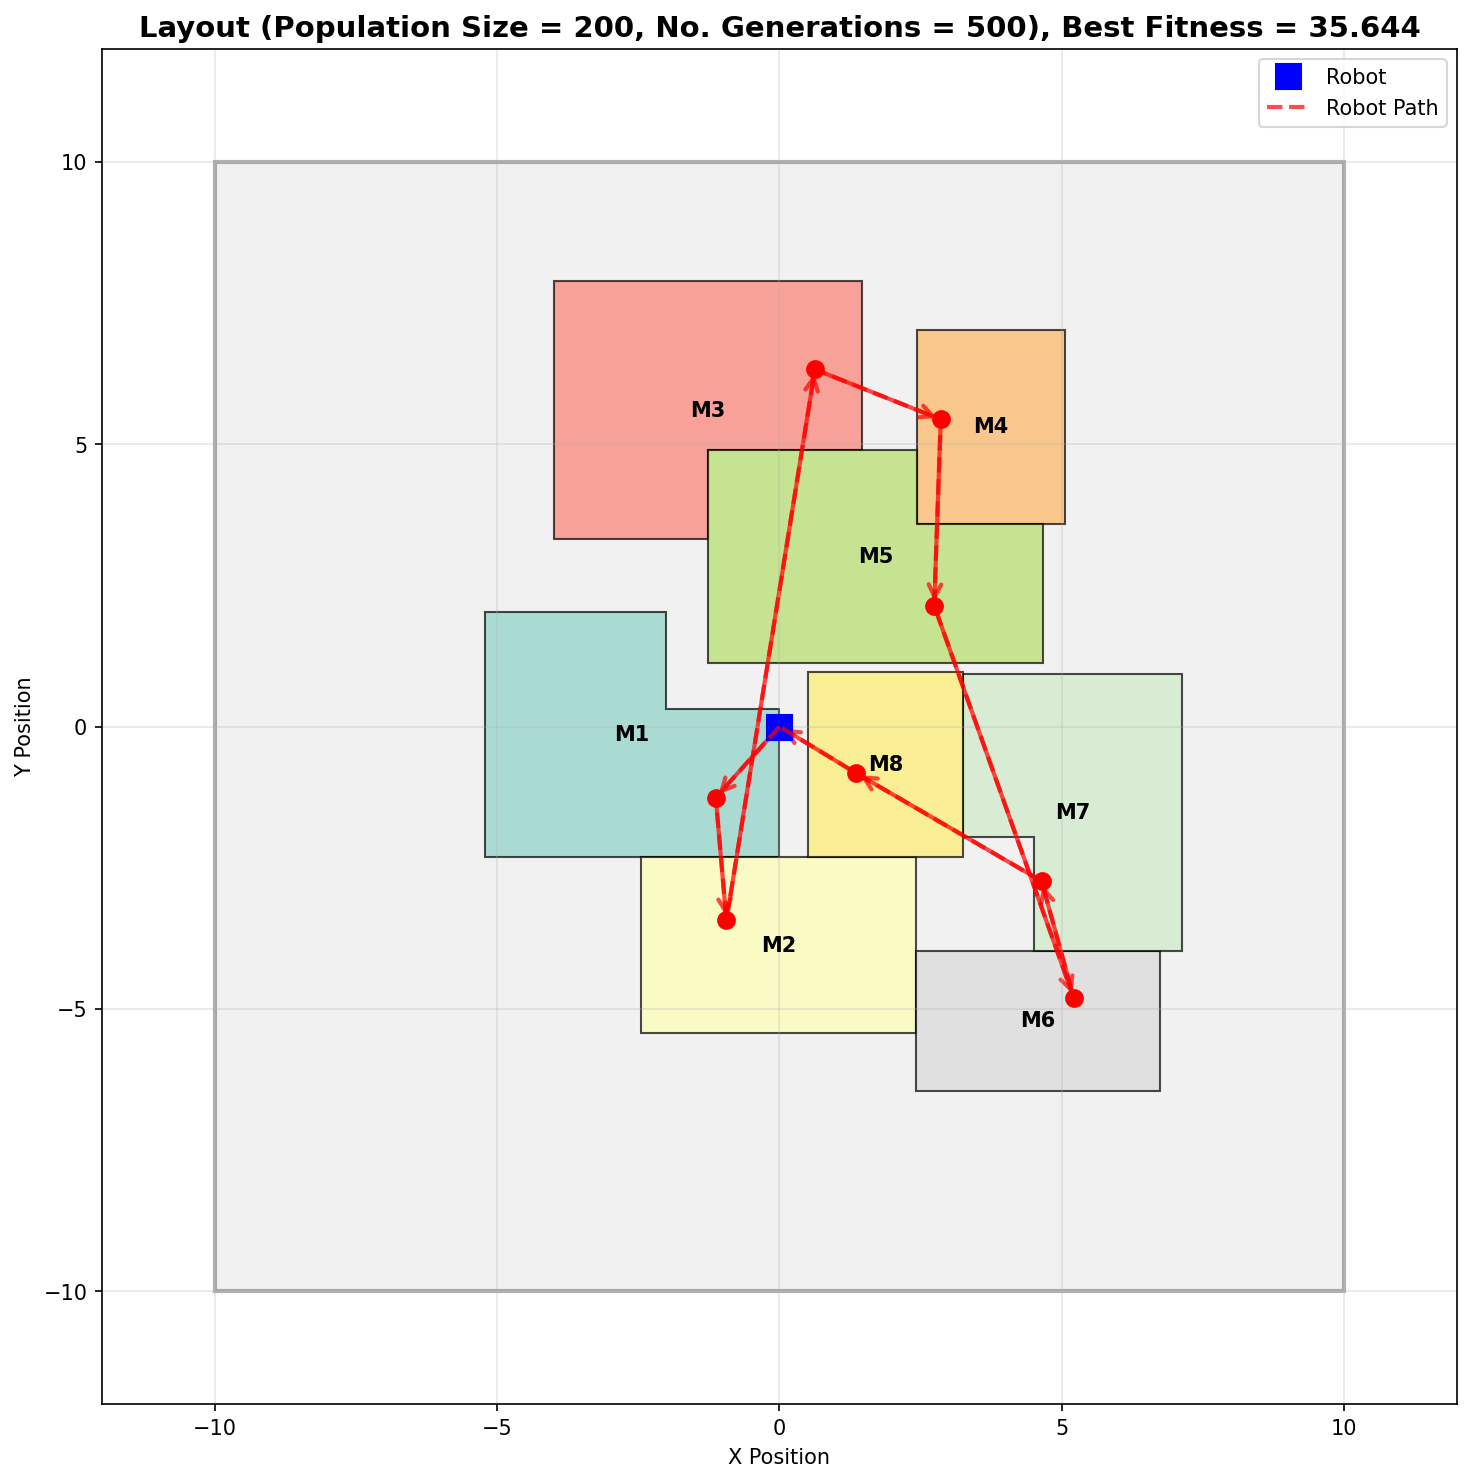
\includegraphics[width=0.7\linewidth]{ga_grid_results_incremental/pop_200/layout_pop_200_gen_500.png}
    \caption{Final optimized layout for population size 200 and 500 generations.}
\end{figure}

\clearpage

\subsubsection{Generations = 1000}
\begin{figure}[H]
    \centering
    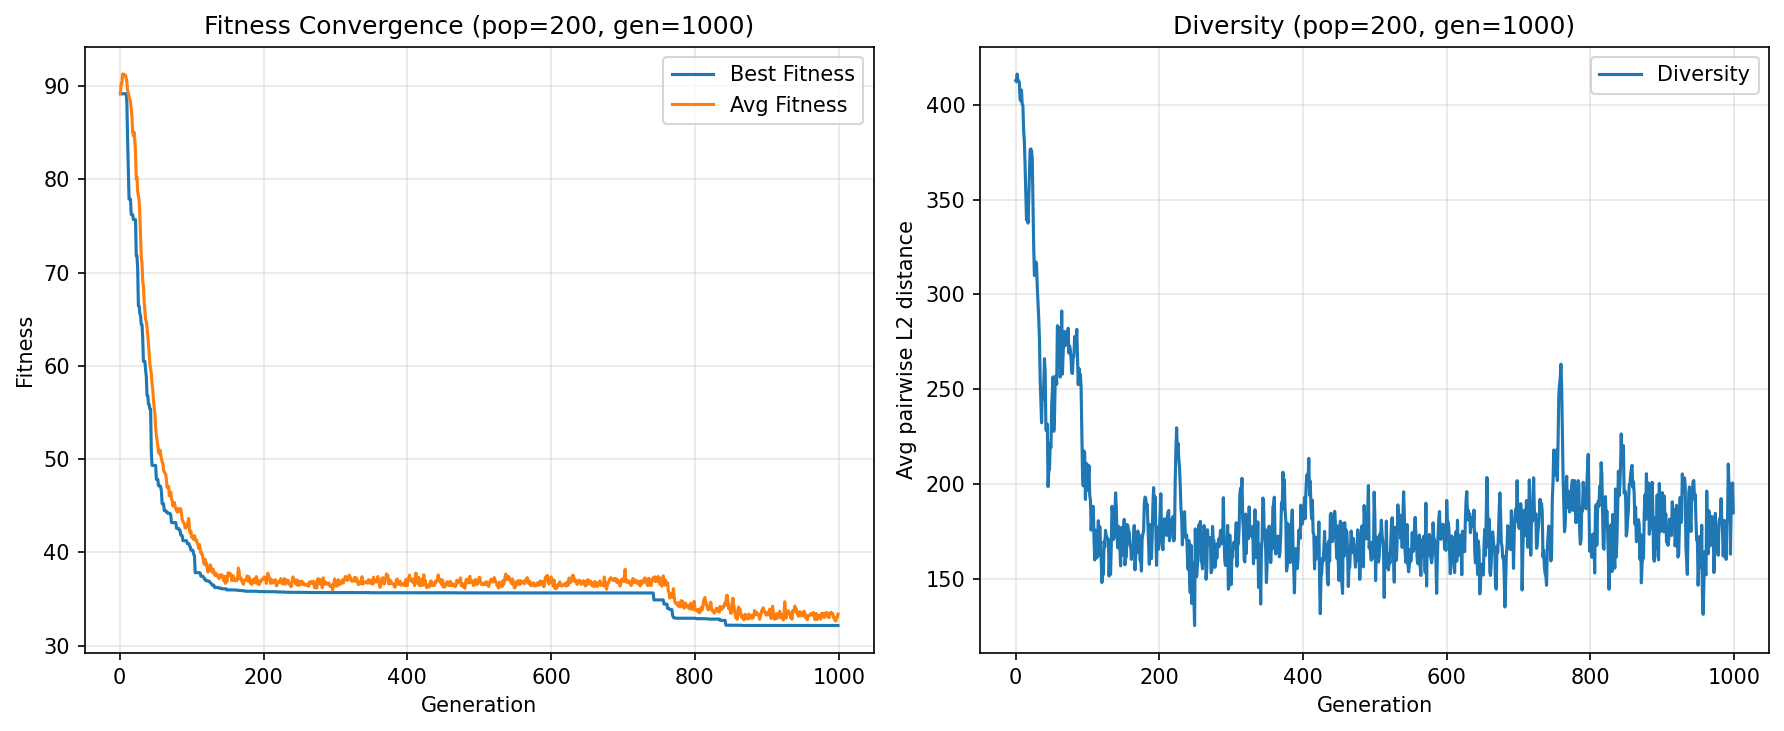
\includegraphics[width=0.9\linewidth]{ga_grid_results_incremental/pop_200/pop_200_gen_1000.png}
    \caption{Fitness convergence and diversity plot for population size 200 and 1000 generations.}
\end{figure}

\begin{figure}[H]
    \centering
    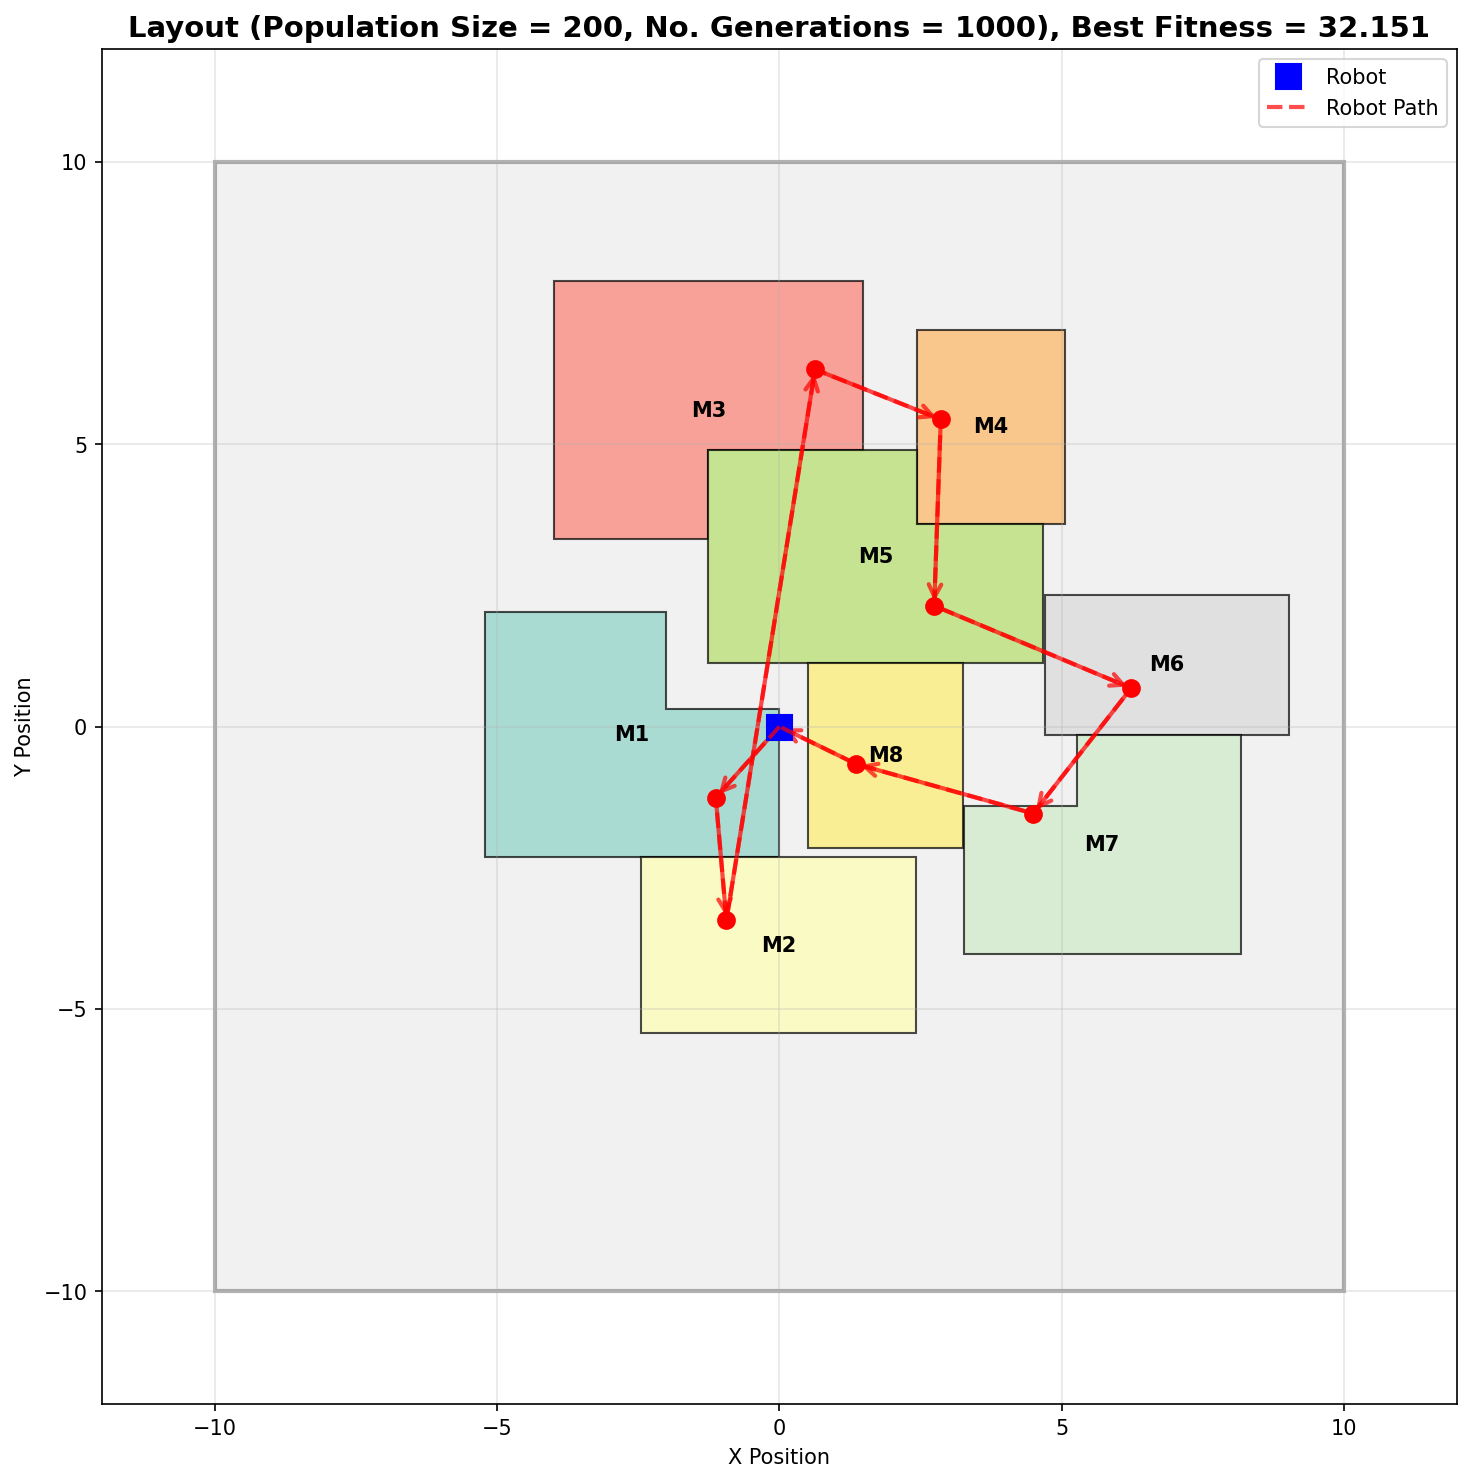
\includegraphics[width=0.7\linewidth]{ga_grid_results_incremental/pop_200/layout_pop_200_gen_1000.png}
    \caption{Final optimized layout for population size 200 and 1000 generations.}
\end{figure}

\clearpage

\subsubsection{Generations = 2000}
\begin{figure}[H]
    \centering
    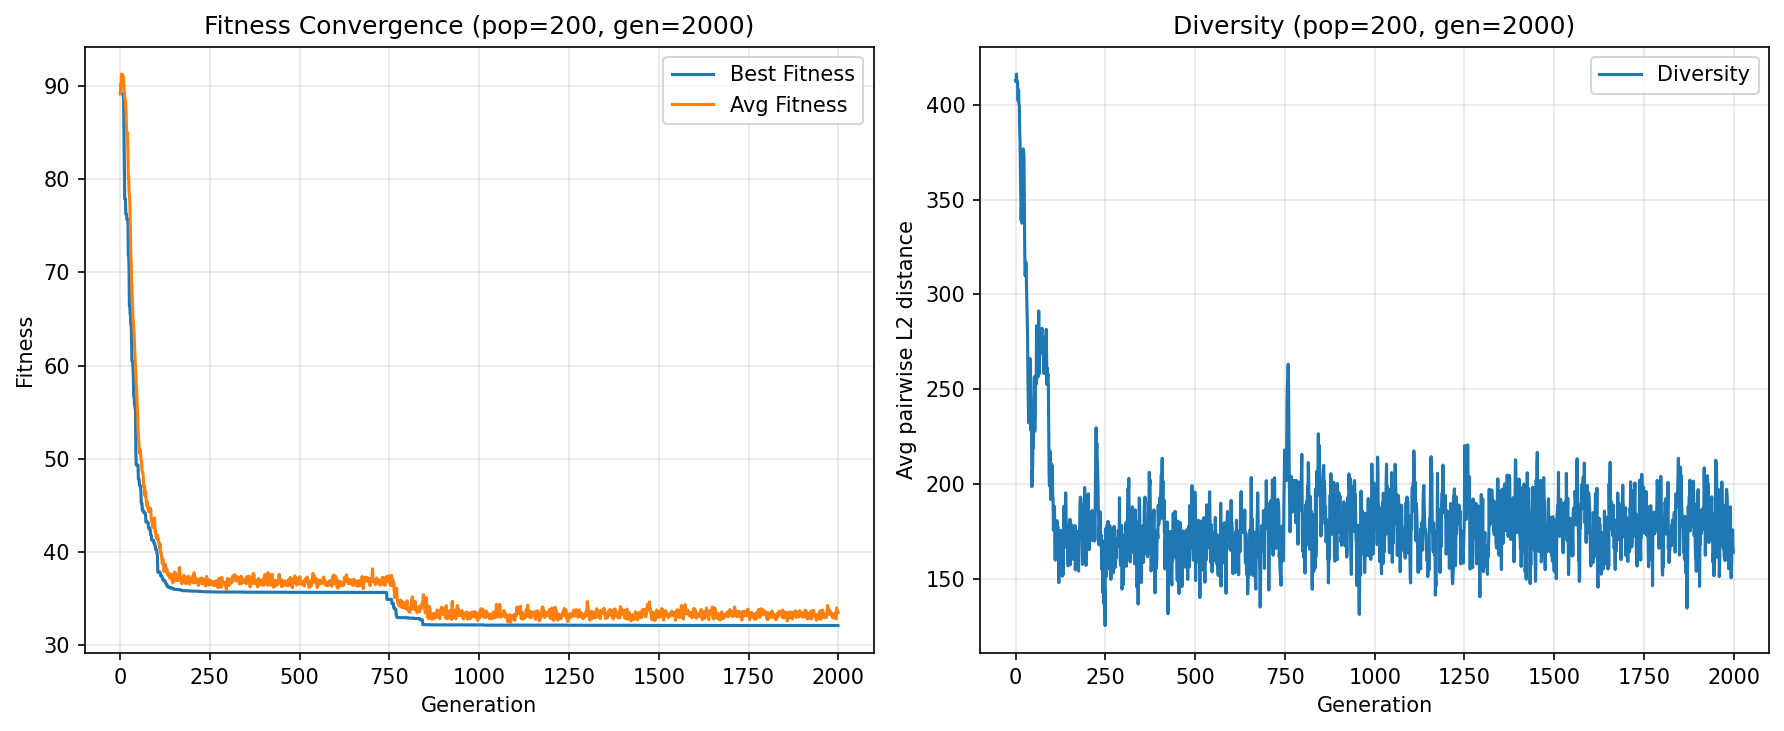
\includegraphics[width=0.9\linewidth]{ga_grid_results_incremental/pop_200/pop_200_gen_2000.png}
    \caption{Fitness convergence and diversity plot for population size 200 and 2000 generations.}
\end{figure}

\begin{figure}[H]
    \centering
    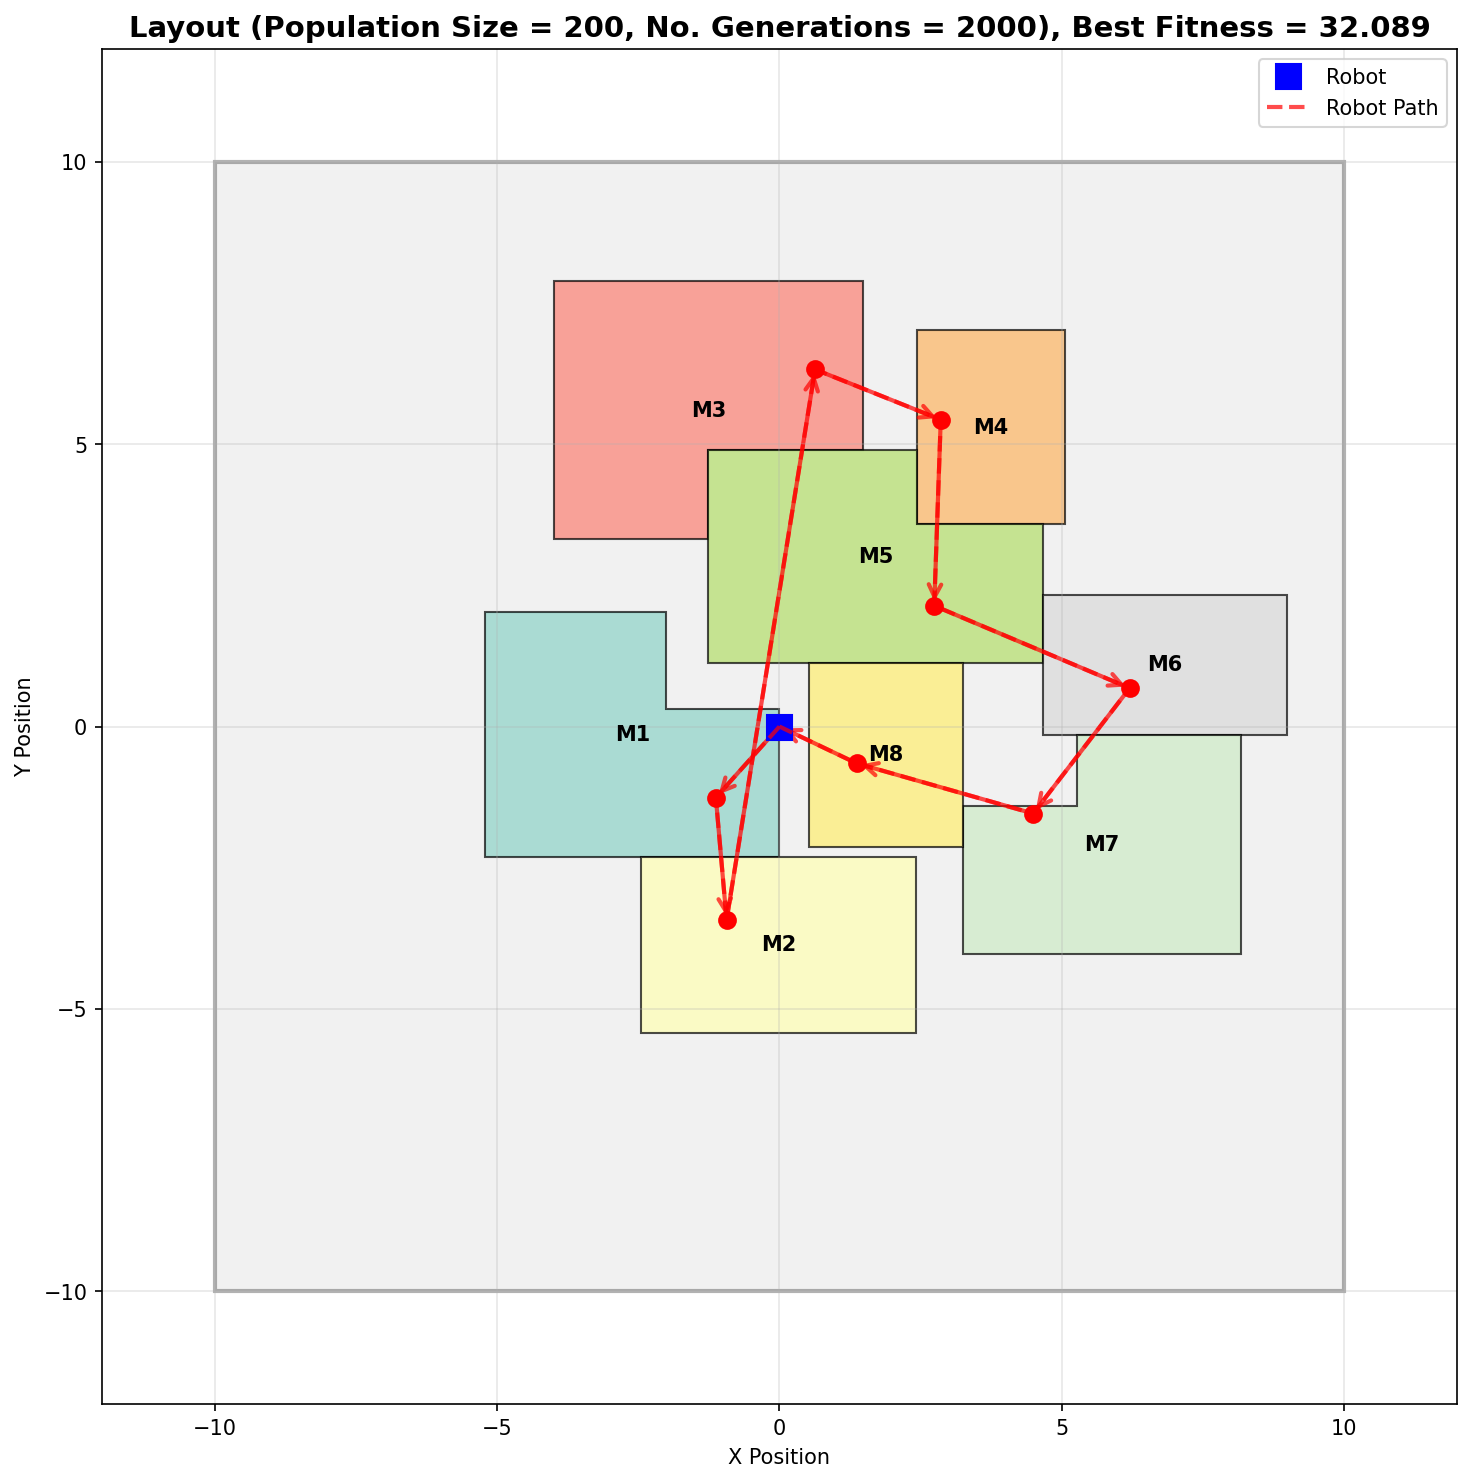
\includegraphics[width=0.7\linewidth]{ga_grid_results_incremental/pop_200/layout_pop_200_gen_2000.png}
    \caption{Final optimized layout for population size 200 and 2000 generations.}
\end{figure}

\clearpage

%====================================================
\subsection{Population Size = 500}
%====================================================

\subsubsection{Generations = 100}
\begin{figure}[H]
    \centering
    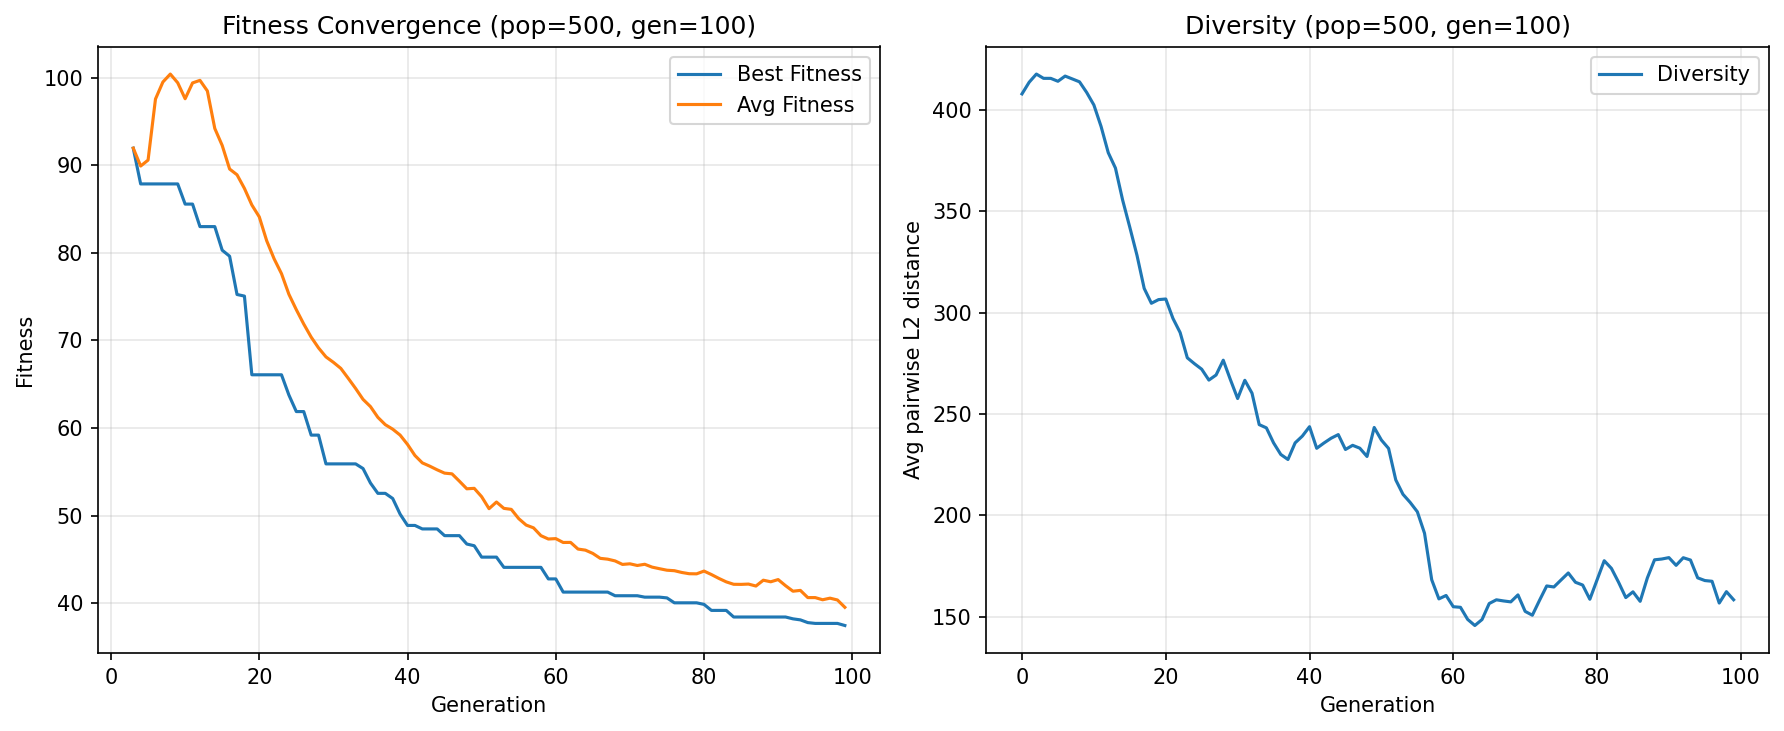
\includegraphics[width=0.9\linewidth]{ga_grid_results_incremental/pop_500/pop_500_gen_100.png}
    \caption{Fitness convergence and diversity plot for population size 500 and 100 generations.}
\end{figure}

\begin{figure}[H]
    \centering
    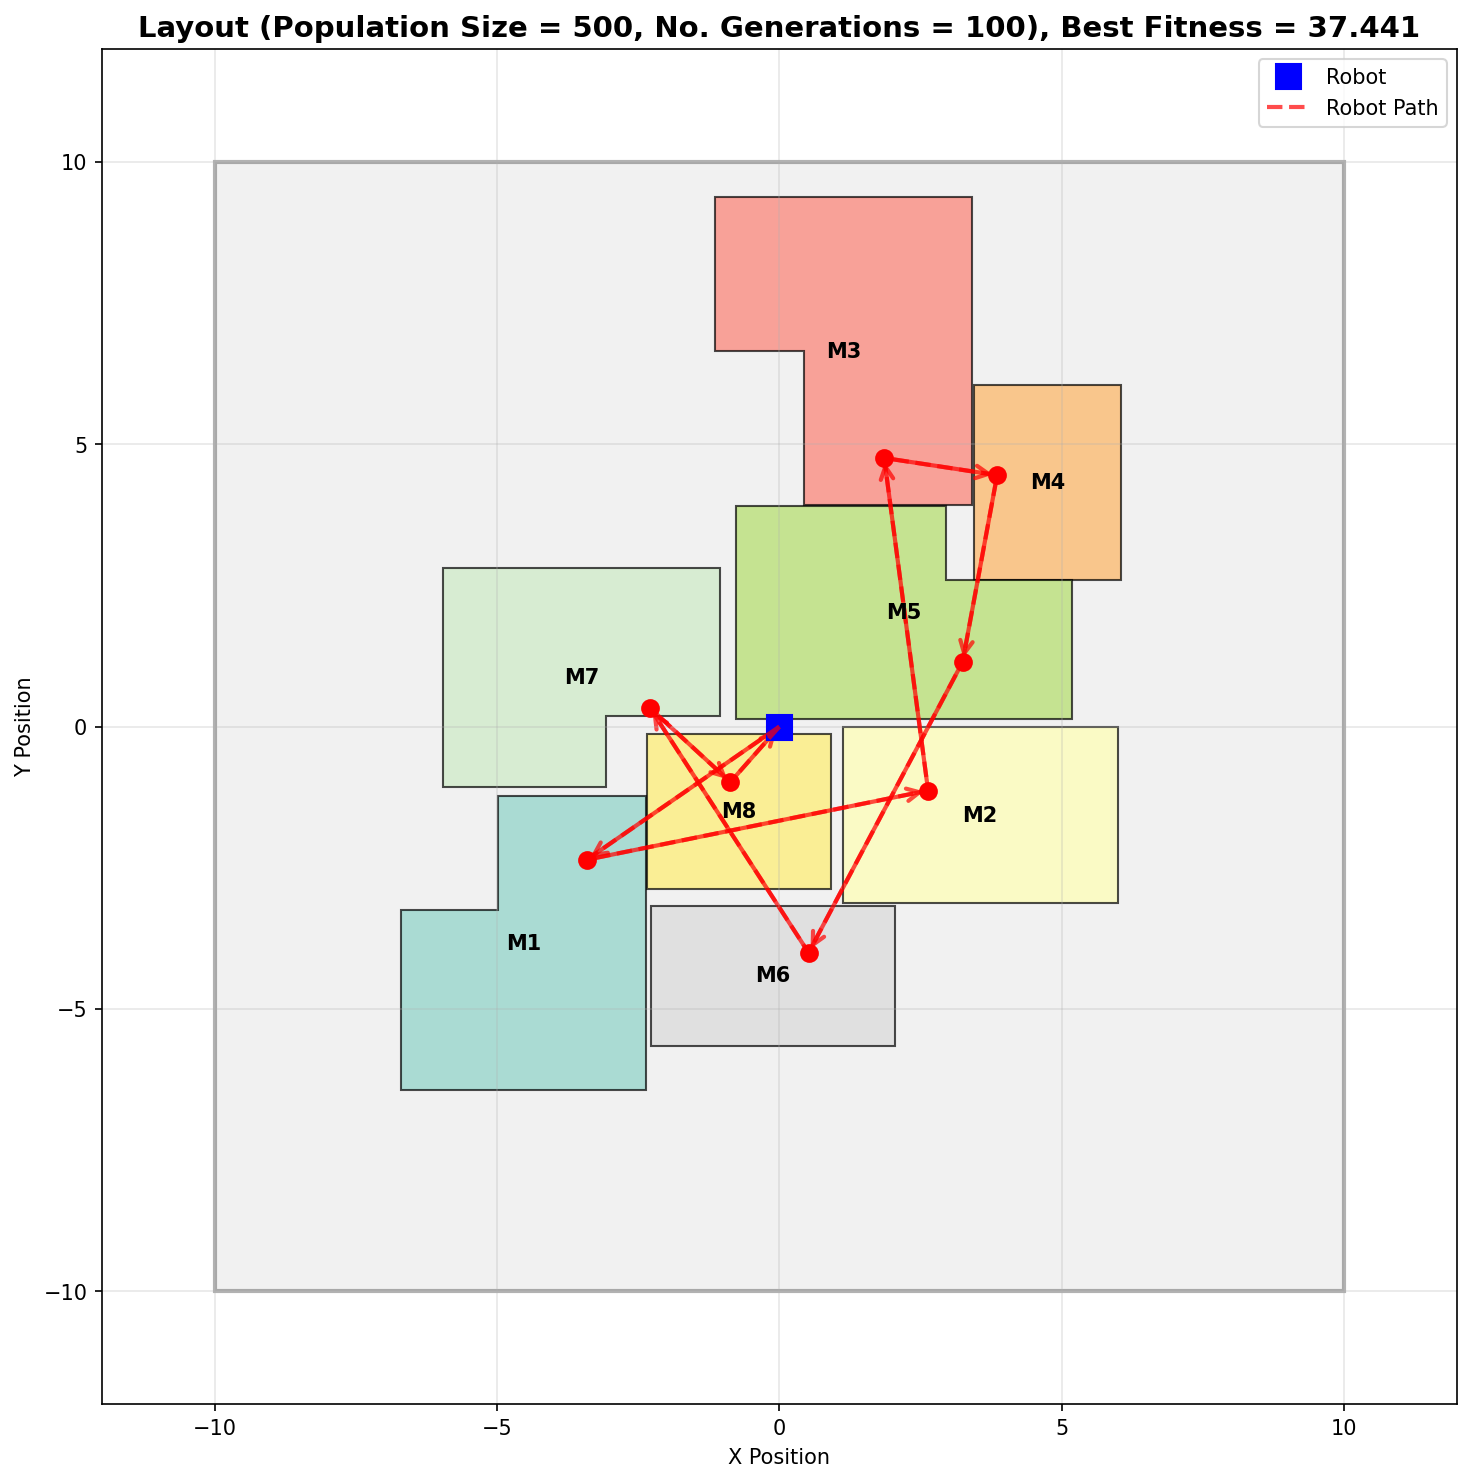
\includegraphics[width=0.7\linewidth]{ga_grid_results_incremental/pop_500/layout_pop_500_gen_100.png}
    \caption{Final optimized layout for population size 500 and 100 generations.}
\end{figure}

\clearpage

\subsubsection{Generations = 200}
\begin{figure}[H]
    \centering
    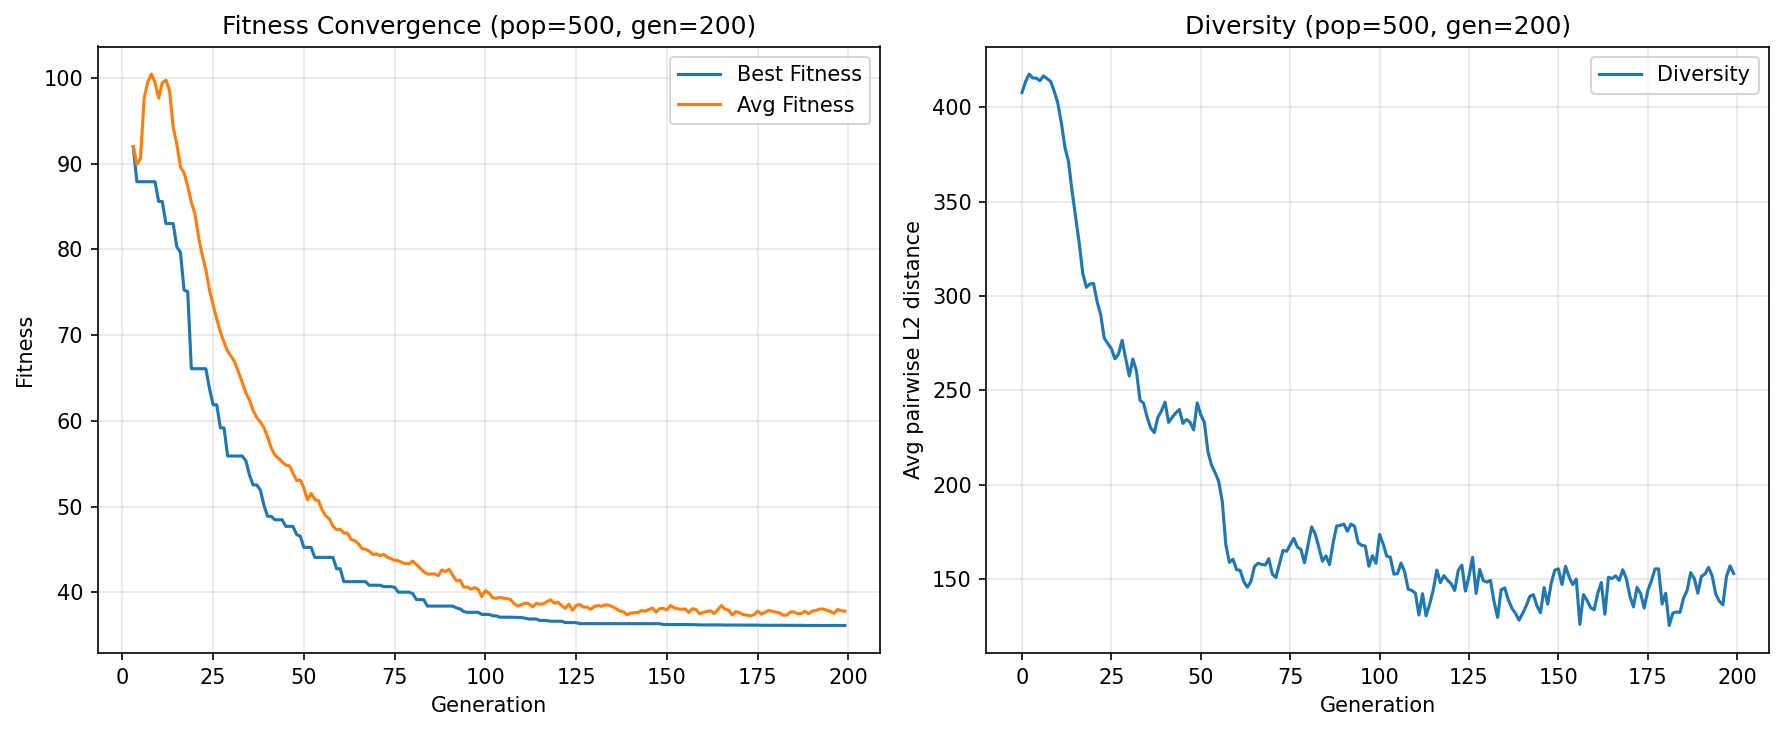
\includegraphics[width=0.9\linewidth]{ga_grid_results_incremental/pop_500/pop_500_gen_200.png}
    \caption{Fitness convergence and diversity plot for population size 500 and 200 generations.}
\end{figure}

\begin{figure}[H]
    \centering
    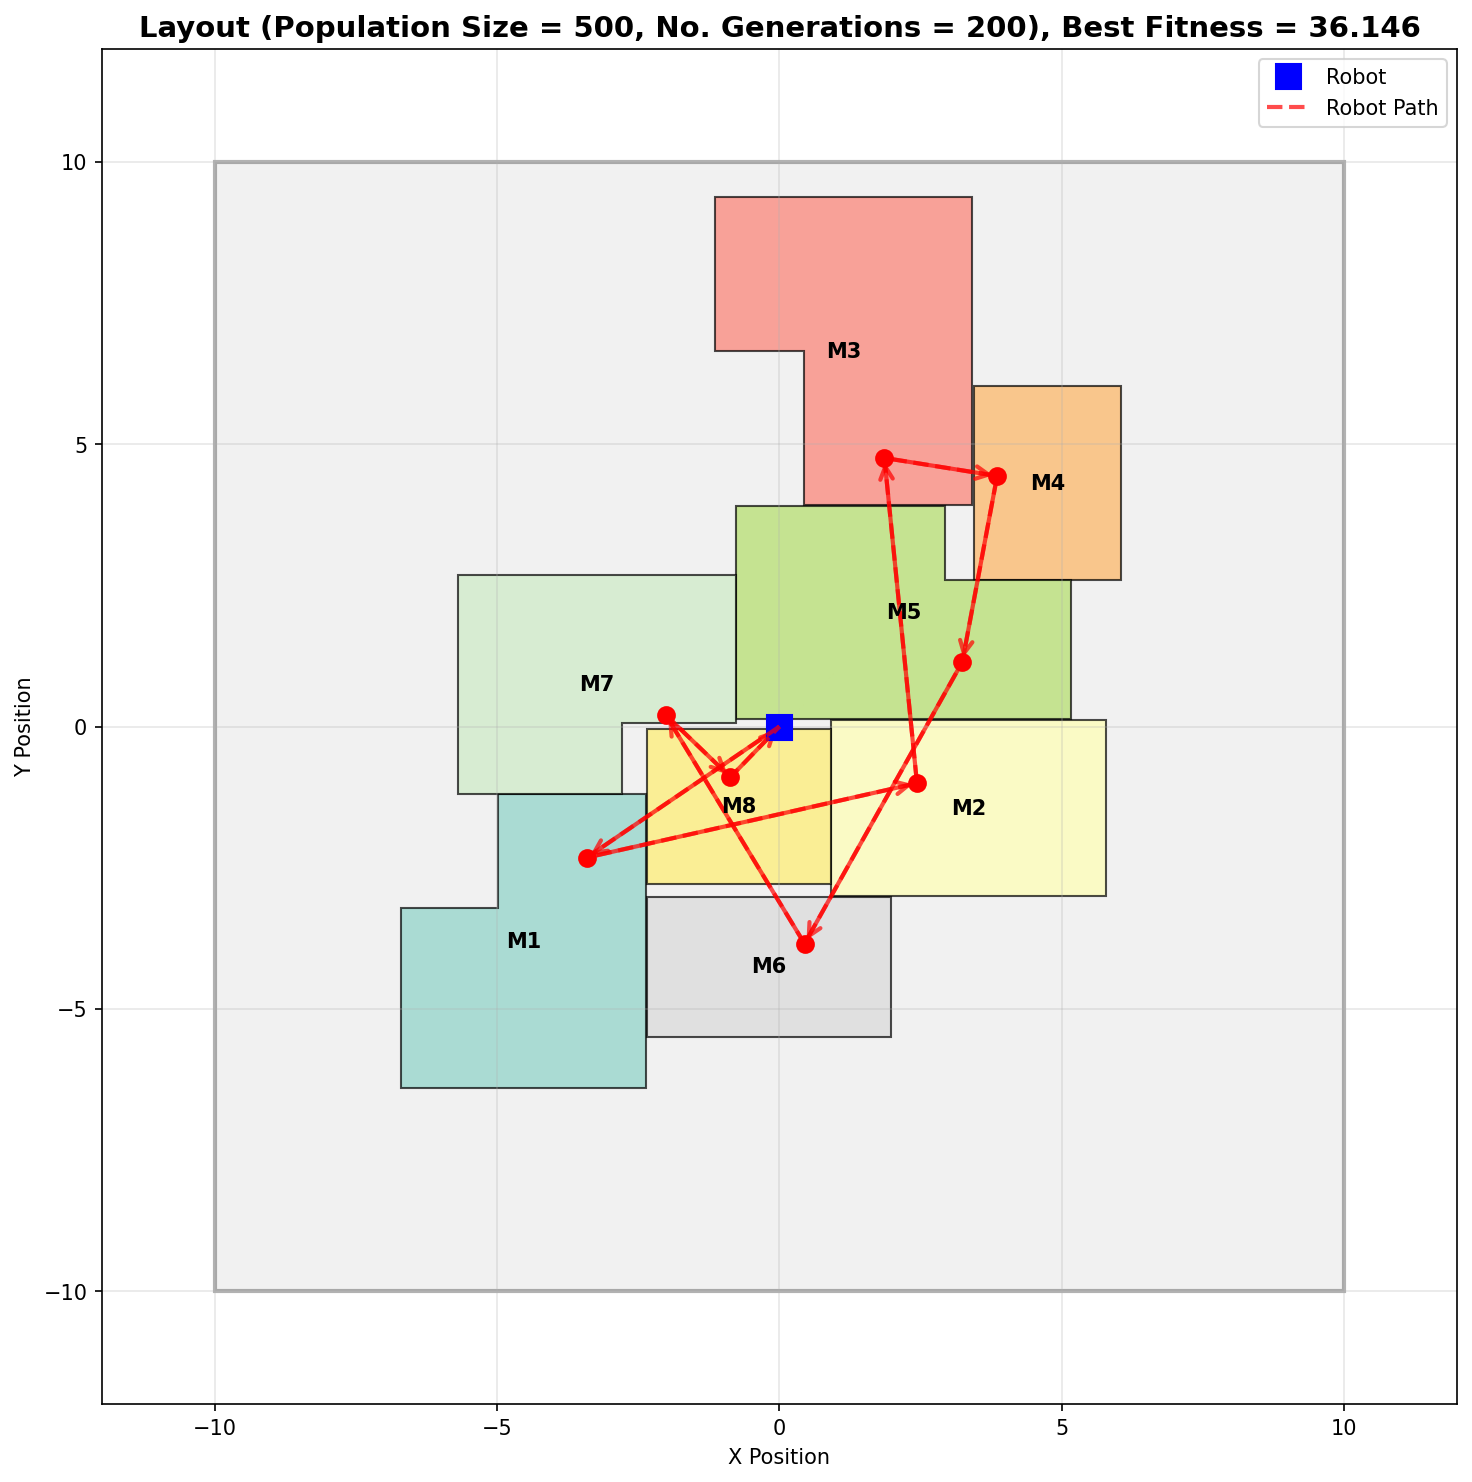
\includegraphics[width=0.7\linewidth]{ga_grid_results_incremental/pop_500/layout_pop_500_gen_200.png}
    \caption{Final optimized layout for population size 500 and 200 generations.}
\end{figure}

\clearpage

\subsubsection{Generations = 500}
\begin{figure}[H]
    \centering
    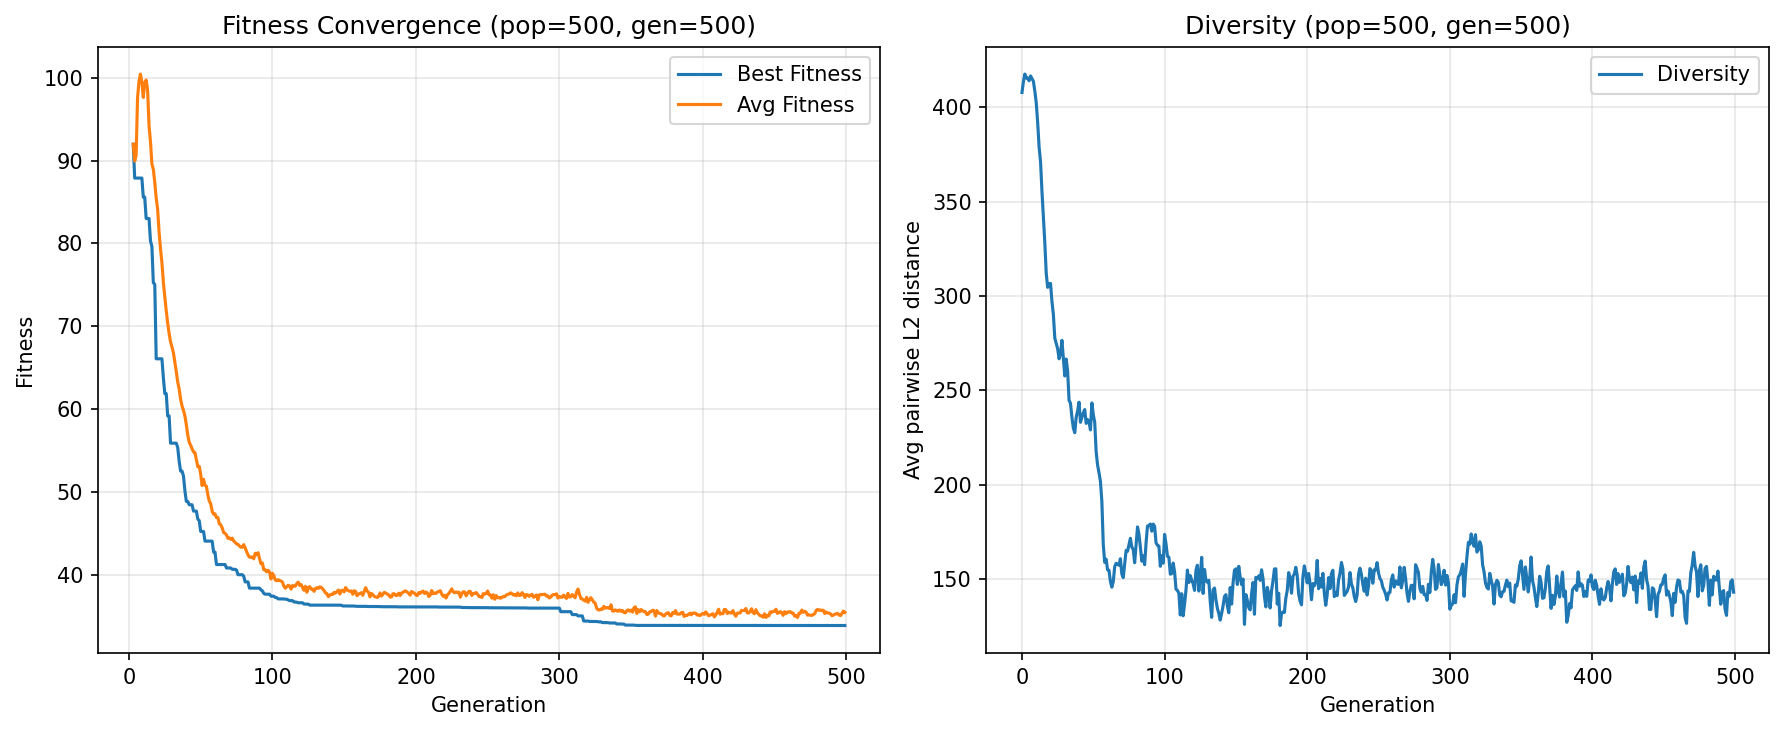
\includegraphics[width=0.9\linewidth]{ga_grid_results_incremental/pop_500/pop_500_gen_500.png}
    \caption{Fitness convergence and diversity plot for population size 500 and 500 generations.}
\end{figure}

\begin{figure}[H]
    \centering
    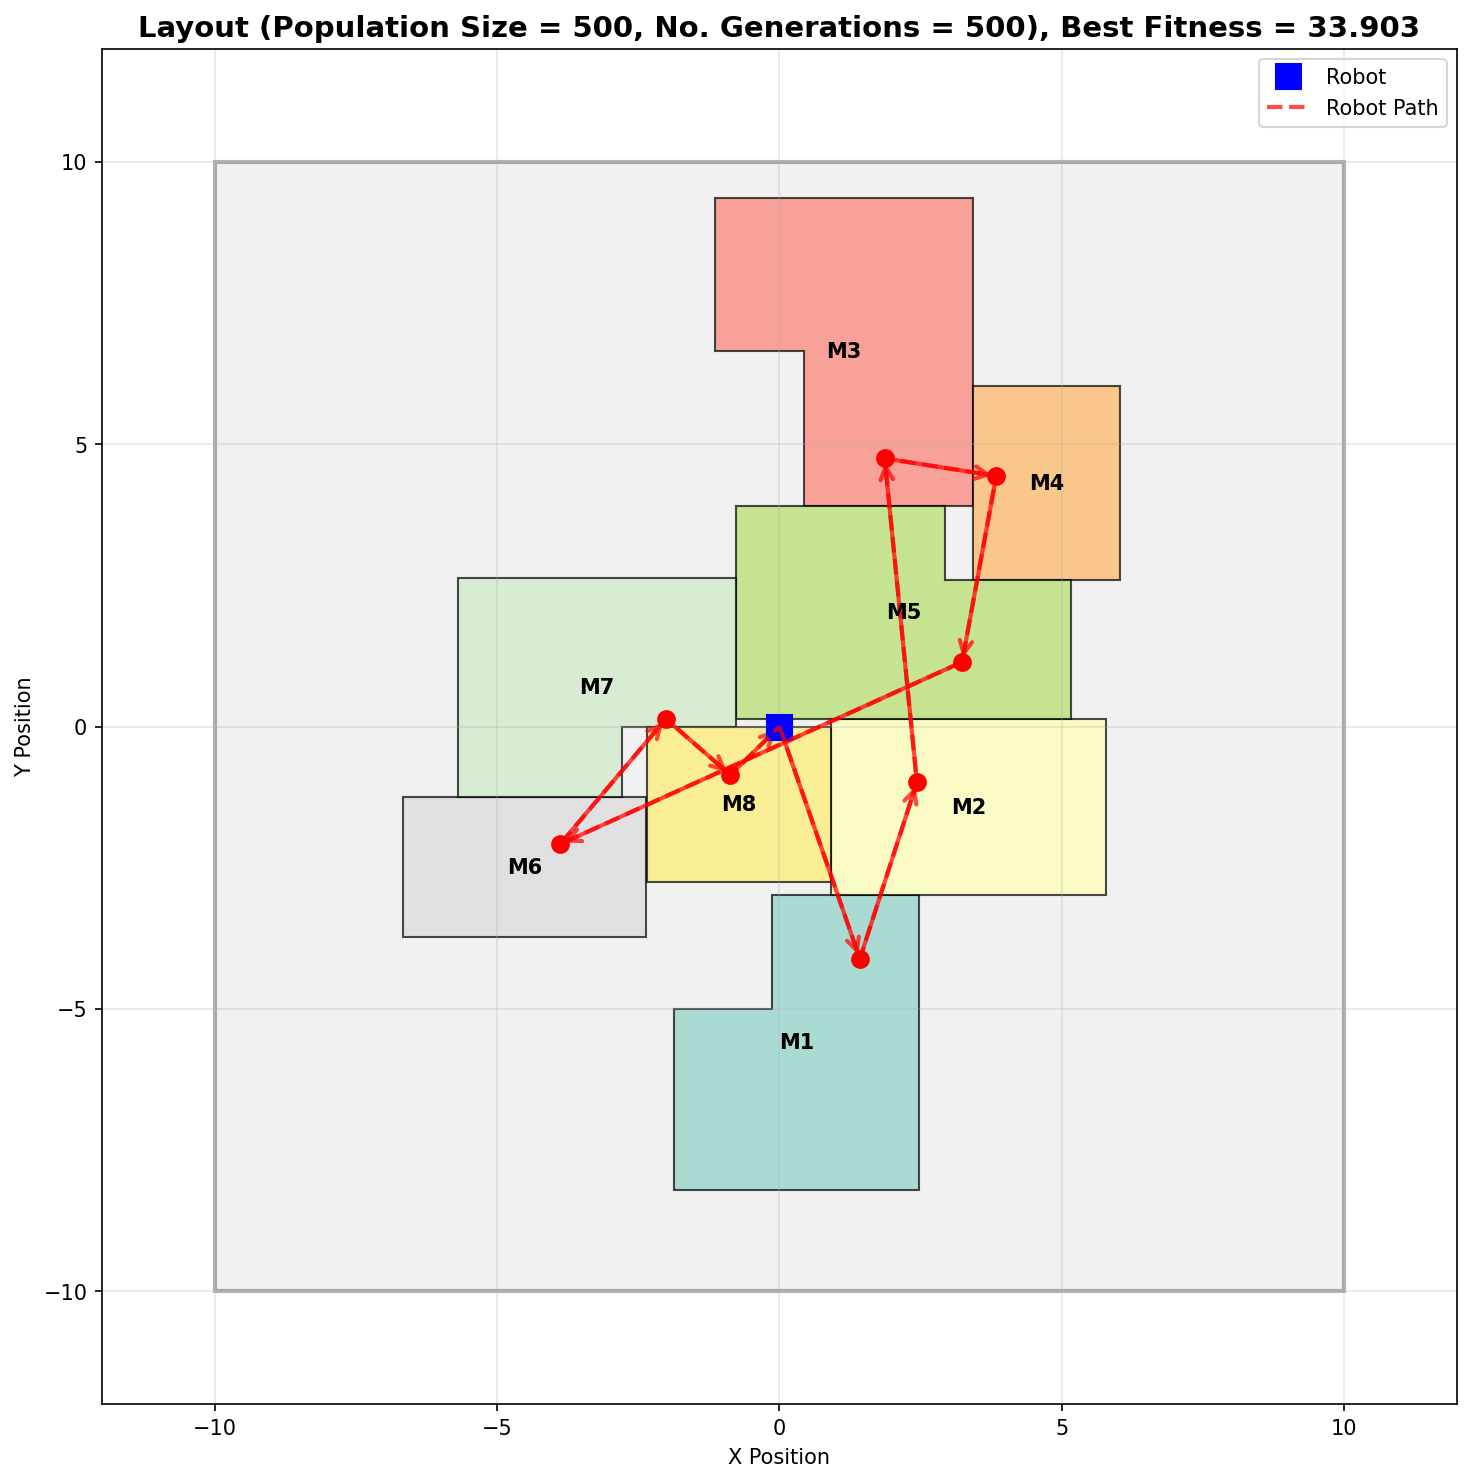
\includegraphics[width=0.7\linewidth]{ga_grid_results_incremental/pop_500/layout_pop_500_gen_500.png}
    \caption{Final optimized layout for population size 500 and 500 generations.}
\end{figure}

\clearpage

\subsubsection{Generations = 1000}
\begin{figure}[H]
    \centering
    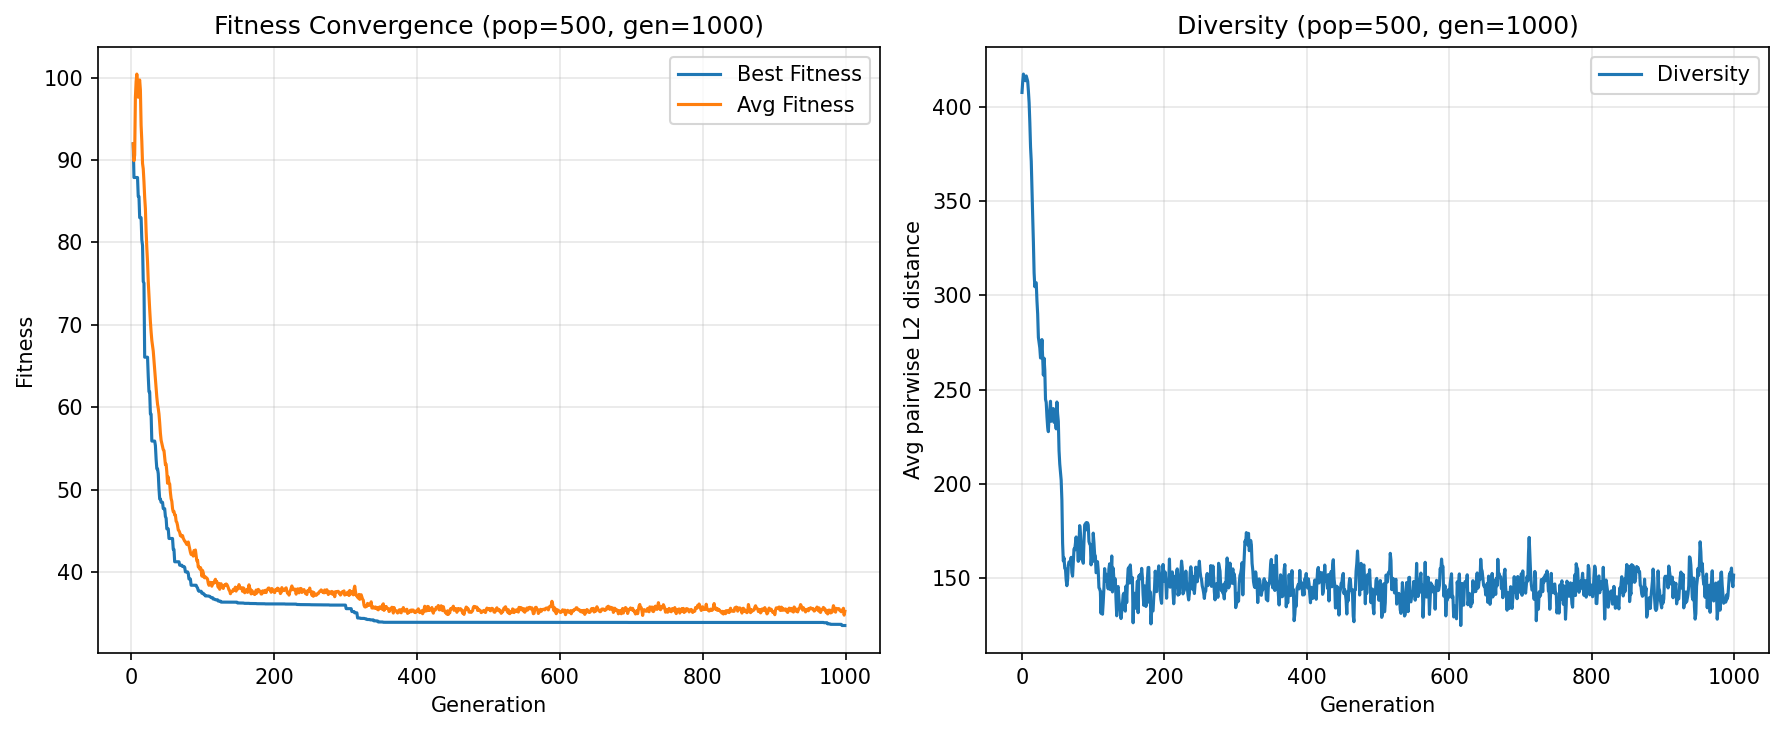
\includegraphics[width=0.9\linewidth]{ga_grid_results_incremental/pop_500/pop_500_gen_1000.png}
    \caption{Fitness convergence and diversity plot for population size 500 and 1000 generations.}
\end{figure}

\begin{figure}[H]
    \centering
    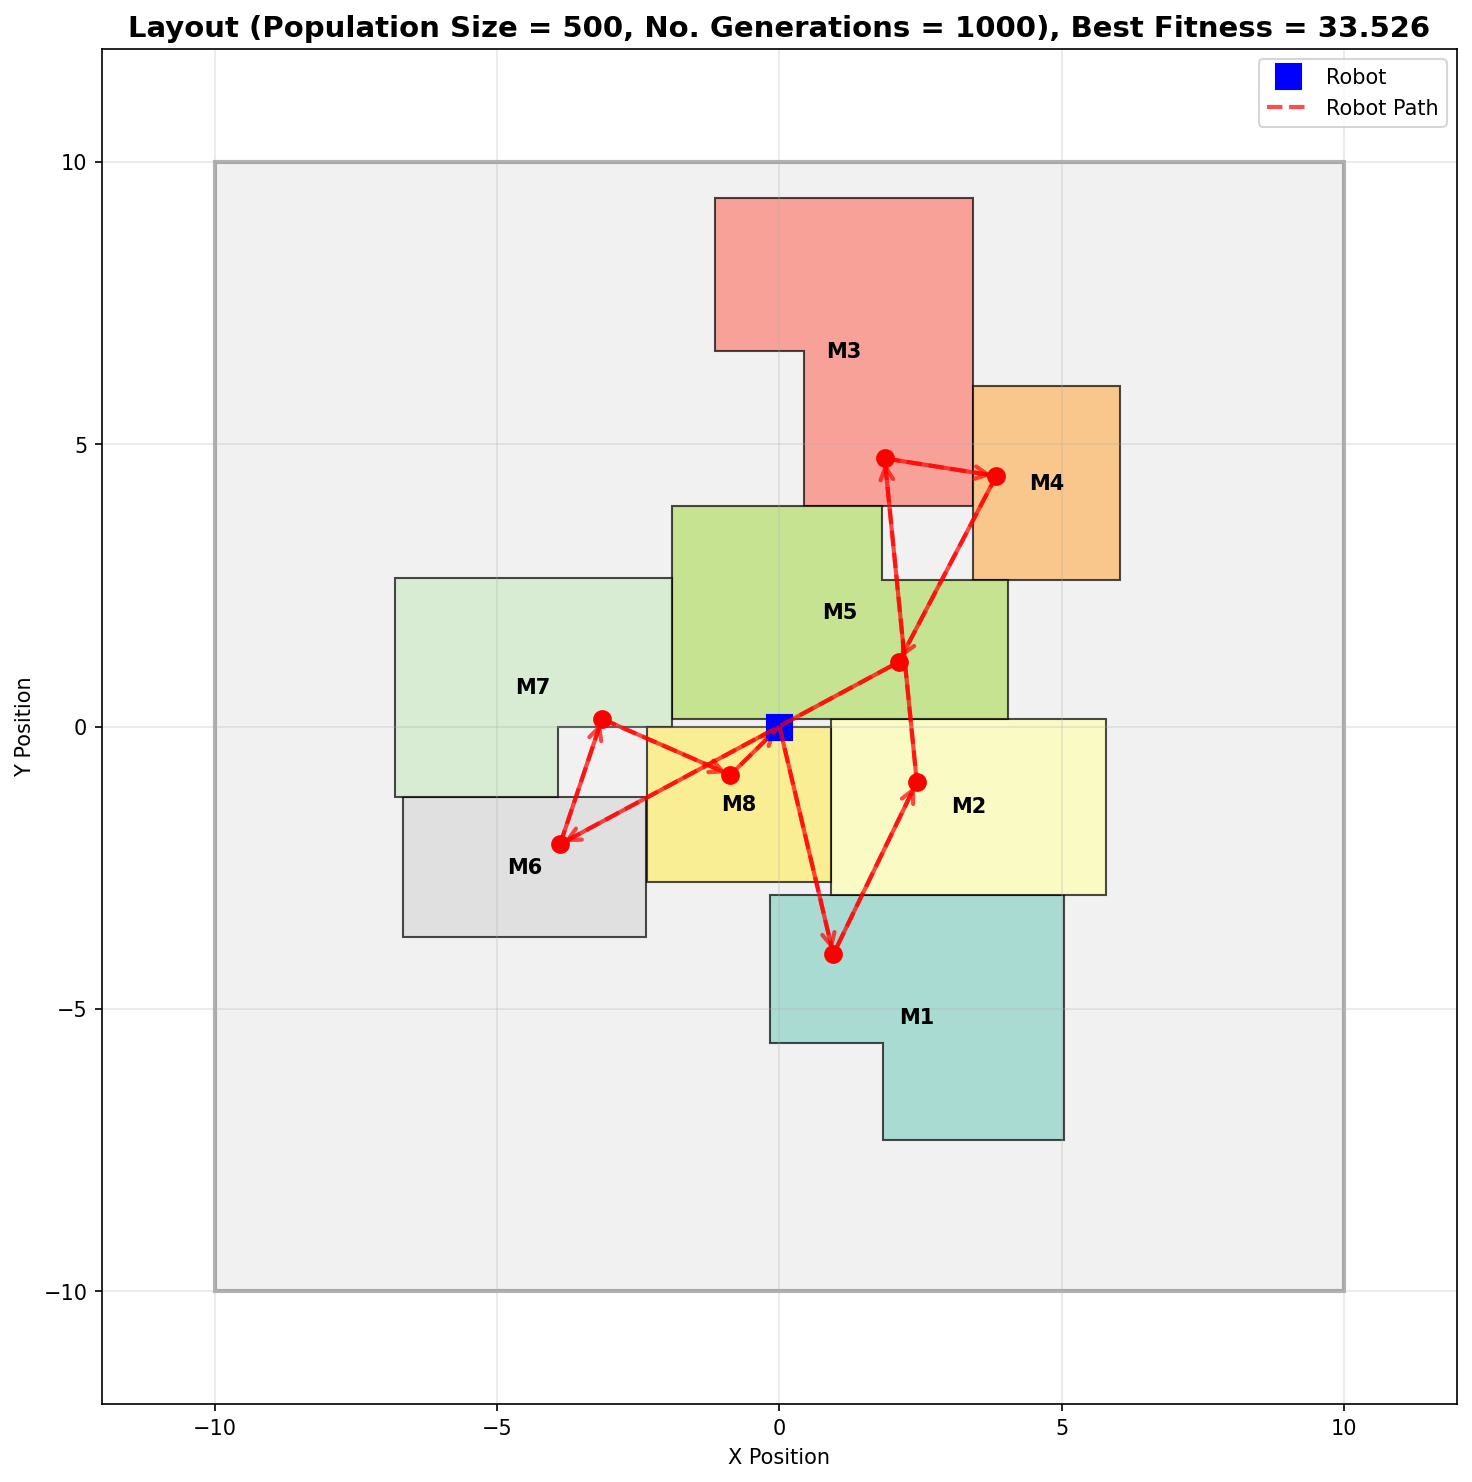
\includegraphics[width=0.7\linewidth]{ga_grid_results_incremental/pop_500/layout_pop_500_gen_1000.png}
    \caption{Final optimized layout for population size 500 and 1000 generations.}
\end{figure}

\clearpage

\subsubsection{Generations = 2000}
\begin{figure}[H]
    \centering
    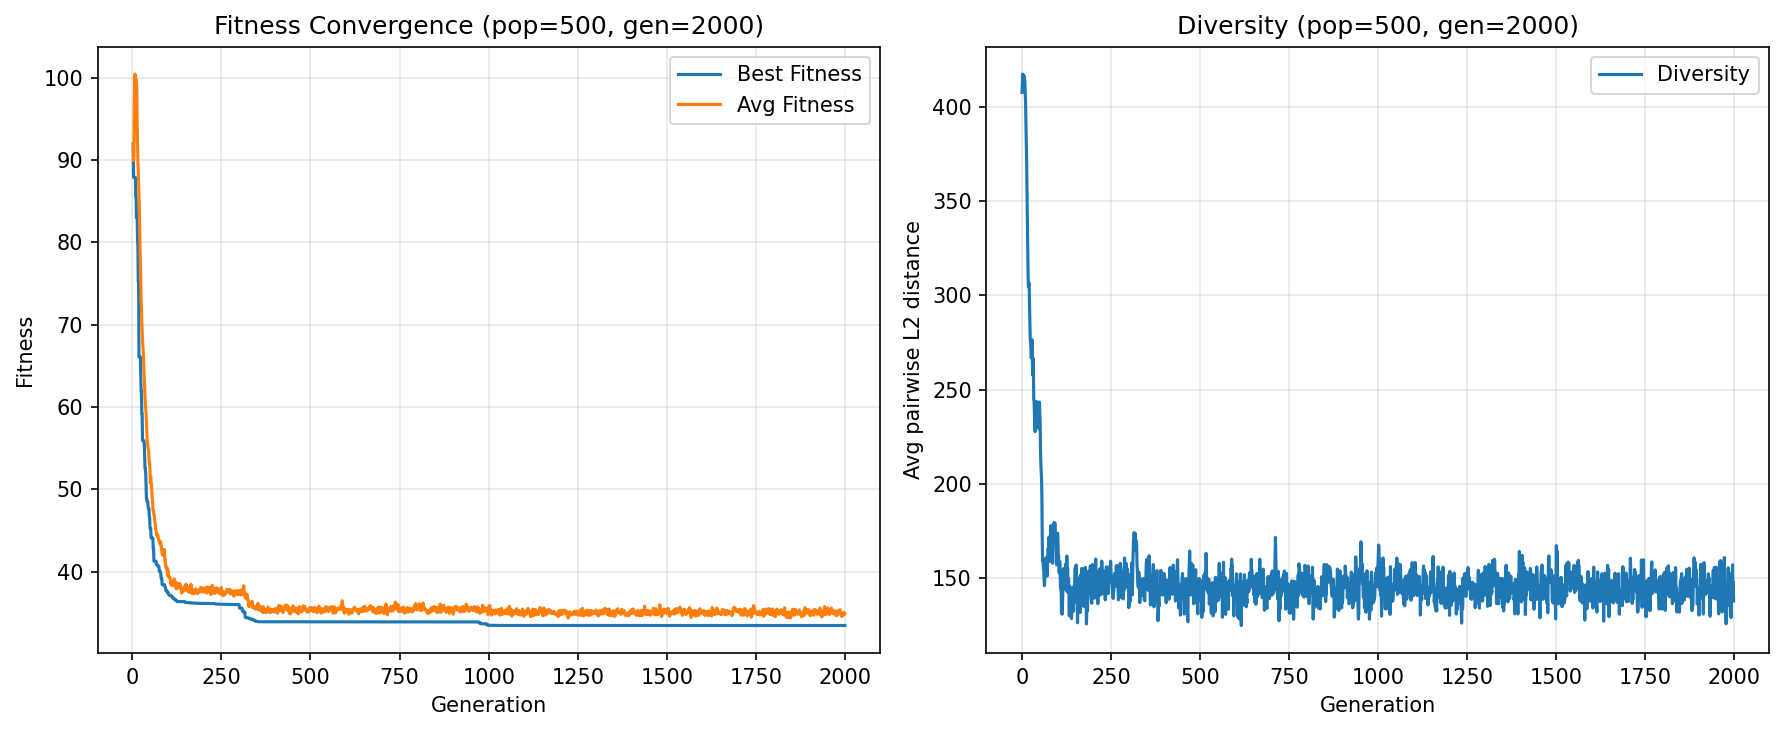
\includegraphics[width=0.9\linewidth]{ga_grid_results_incremental/pop_500/pop_500_gen_2000.png}
    \caption{Fitness convergence and diversity plot for population size 500 and 2000 generations.}
\end{figure}

\begin{figure}[H]
    \centering
    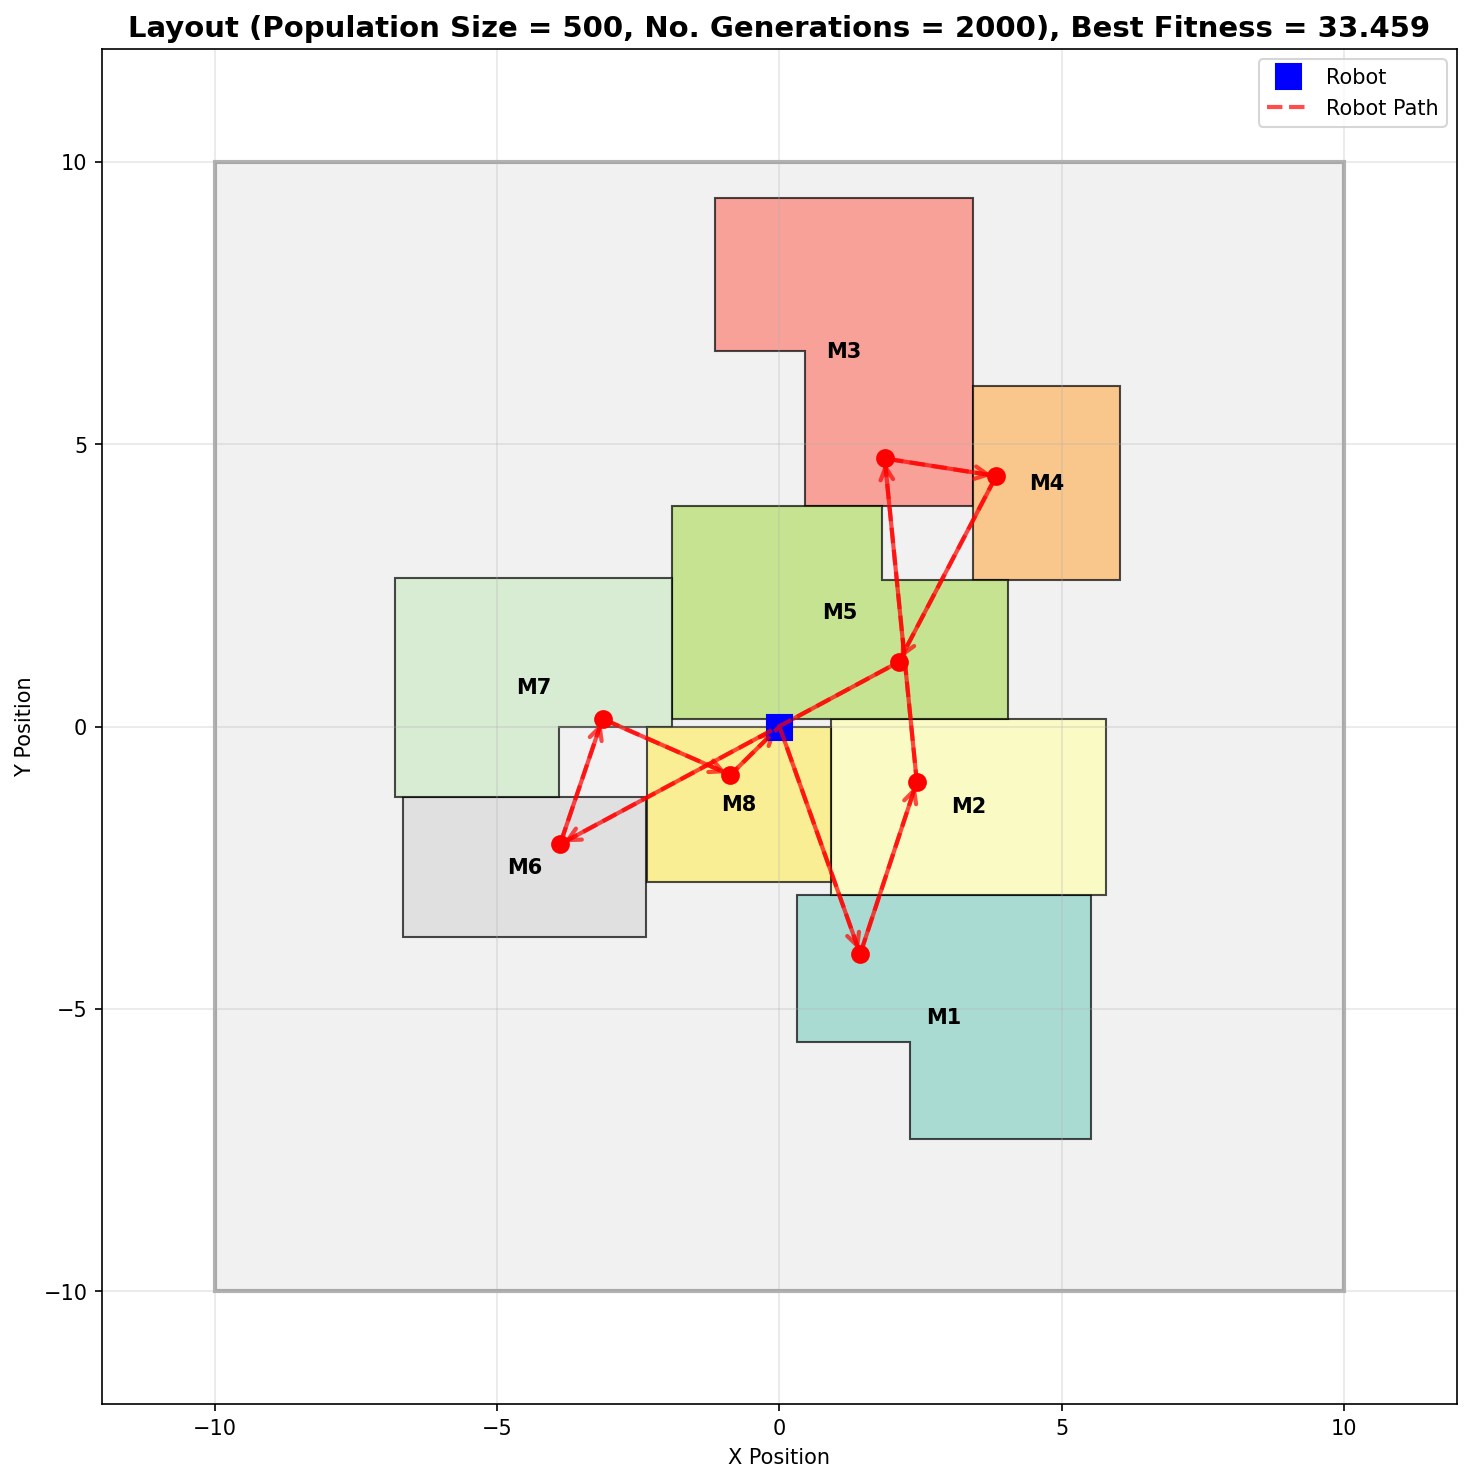
\includegraphics[width=0.7\linewidth]{ga_grid_results_incremental/pop_500/layout_pop_500_gen_2000.png}
    \caption{Final optimized layout for population size 500 and 2000 generations.}
\end{figure}

\clearpage

%====================================================
\subsection{Population Size = 1000}
%====================================================

\subsubsection{Generations = 100}
\begin{figure}[H]
    \centering
    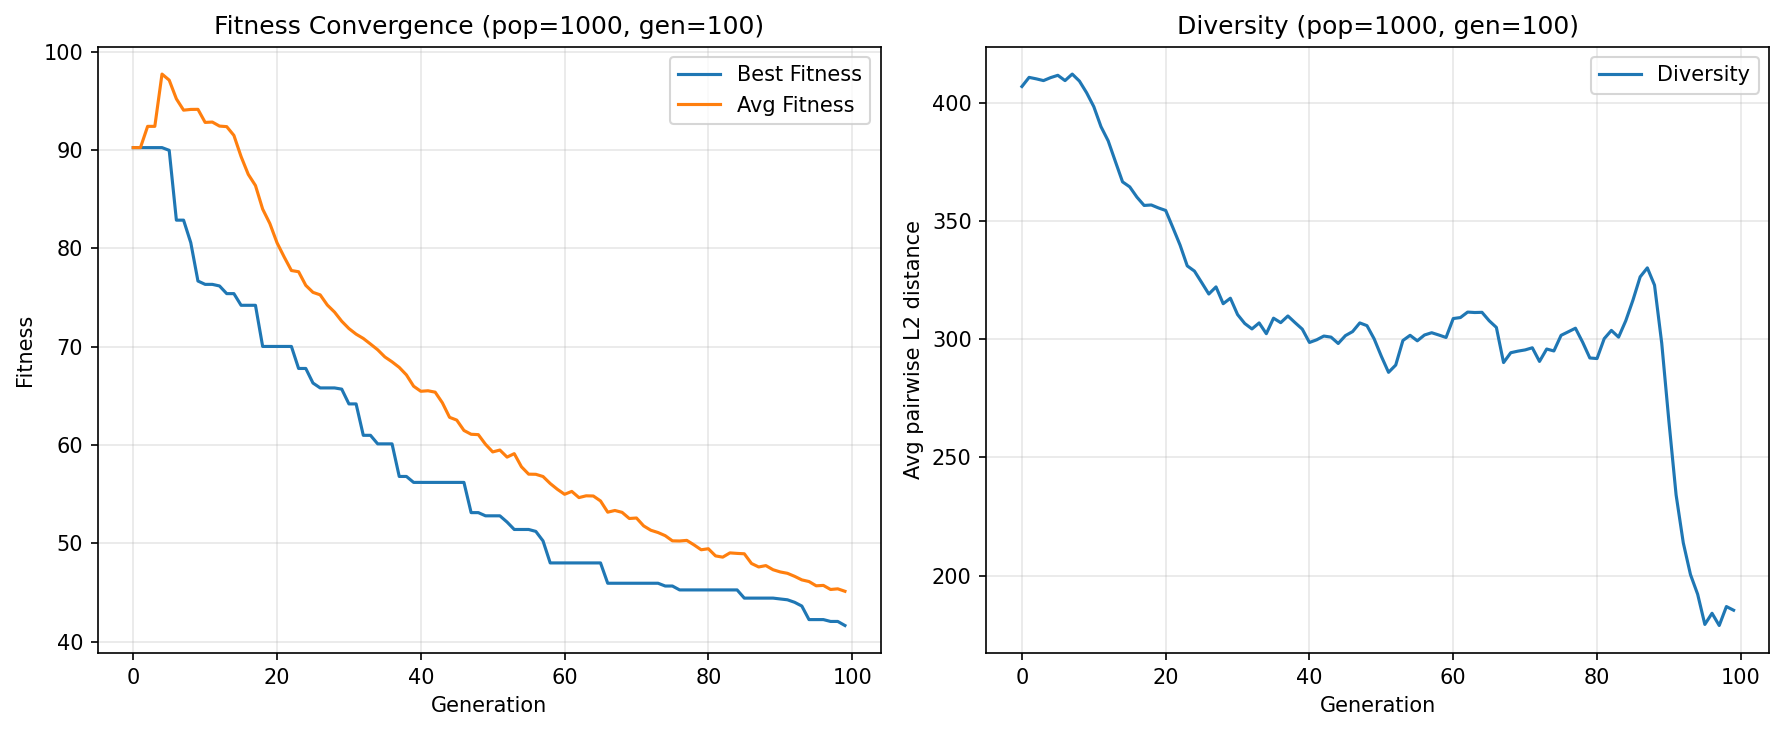
\includegraphics[width=0.9\linewidth]{ga_grid_results_incremental/pop_1000/pop_1000_gen_100.png}
    \caption{Fitness convergence and diversity plot for population size 1000 and 100 generations.}
\end{figure}

\begin{figure}[H]
    \centering
    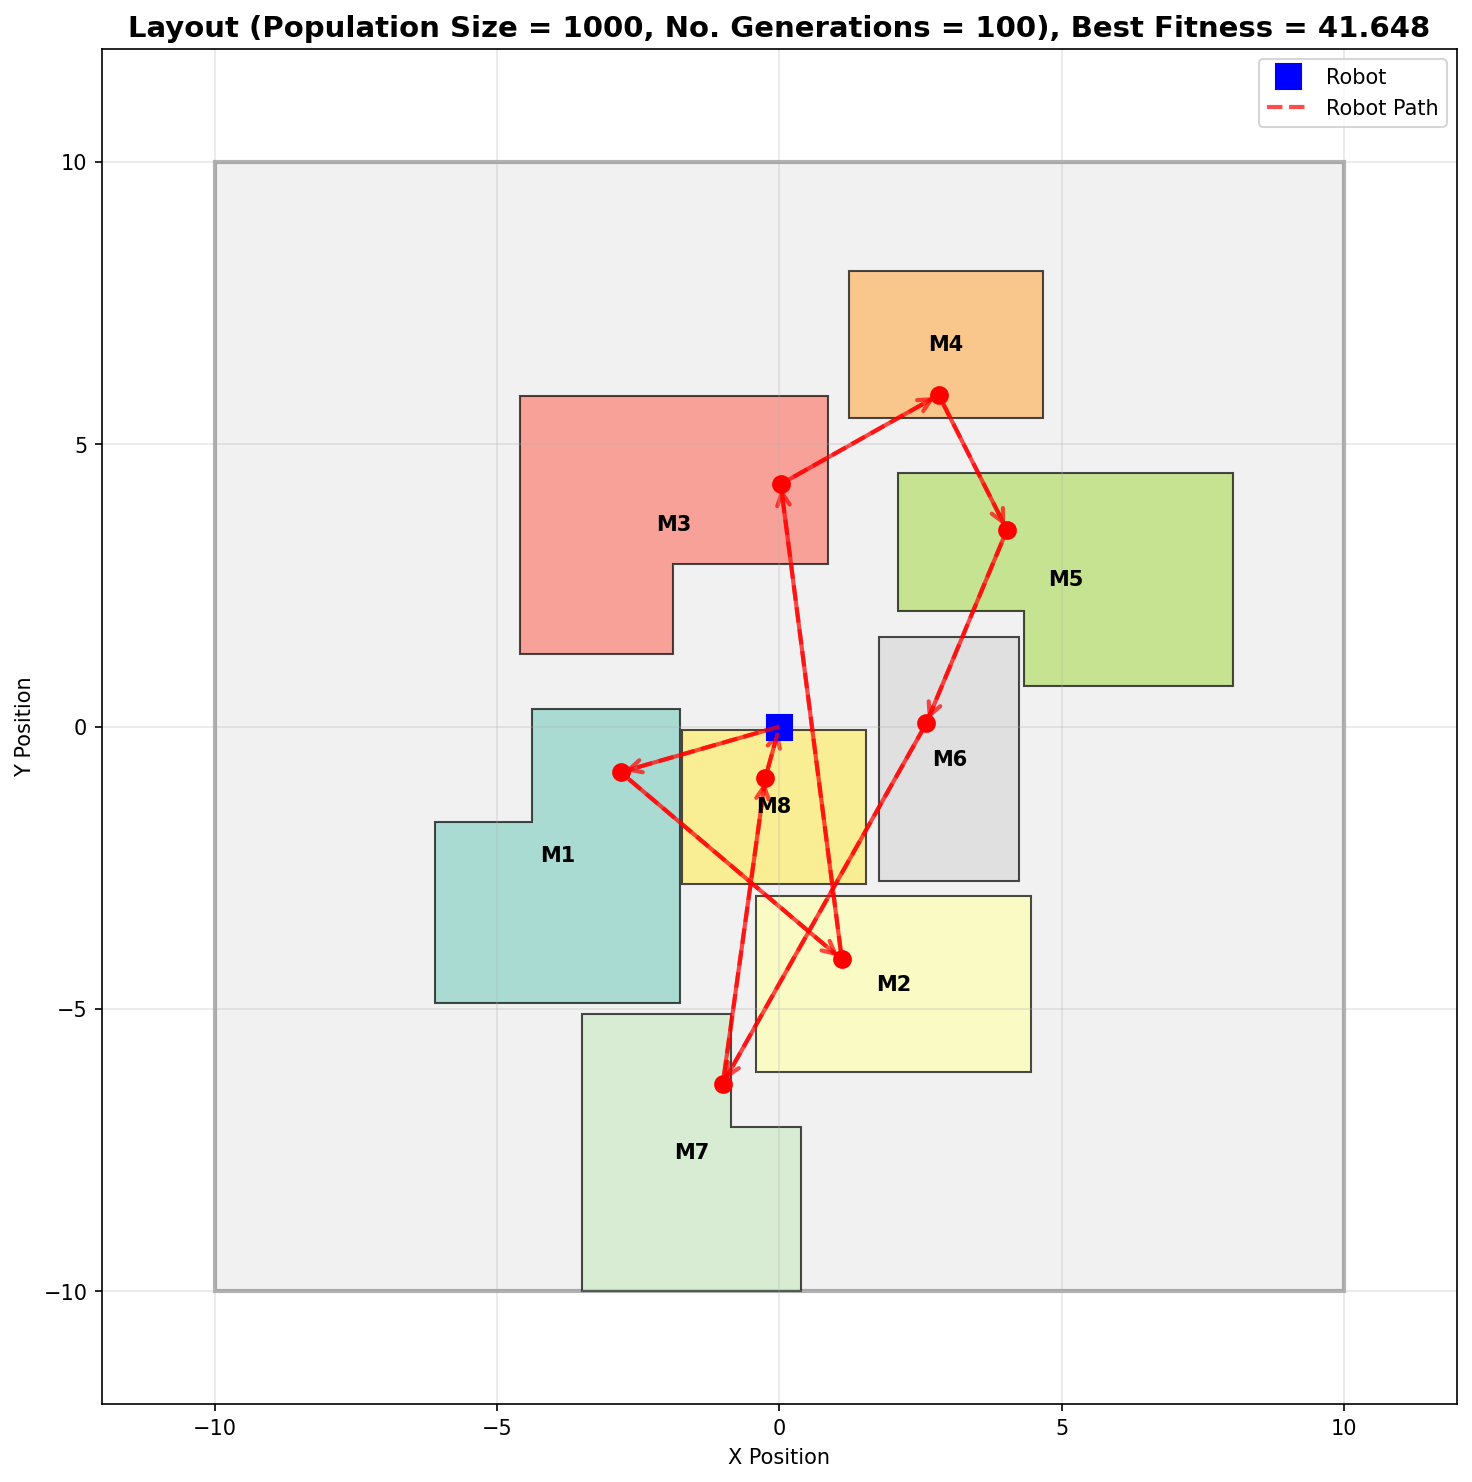
\includegraphics[width=0.7\linewidth]{ga_grid_results_incremental/pop_1000/layout_pop_1000_gen_100.png}
    \caption{Final optimized layout for population size 1000 and 100 generations.}
\end{figure}

\clearpage

\subsubsection{Generations = 200}
\begin{figure}[H]
    \centering
    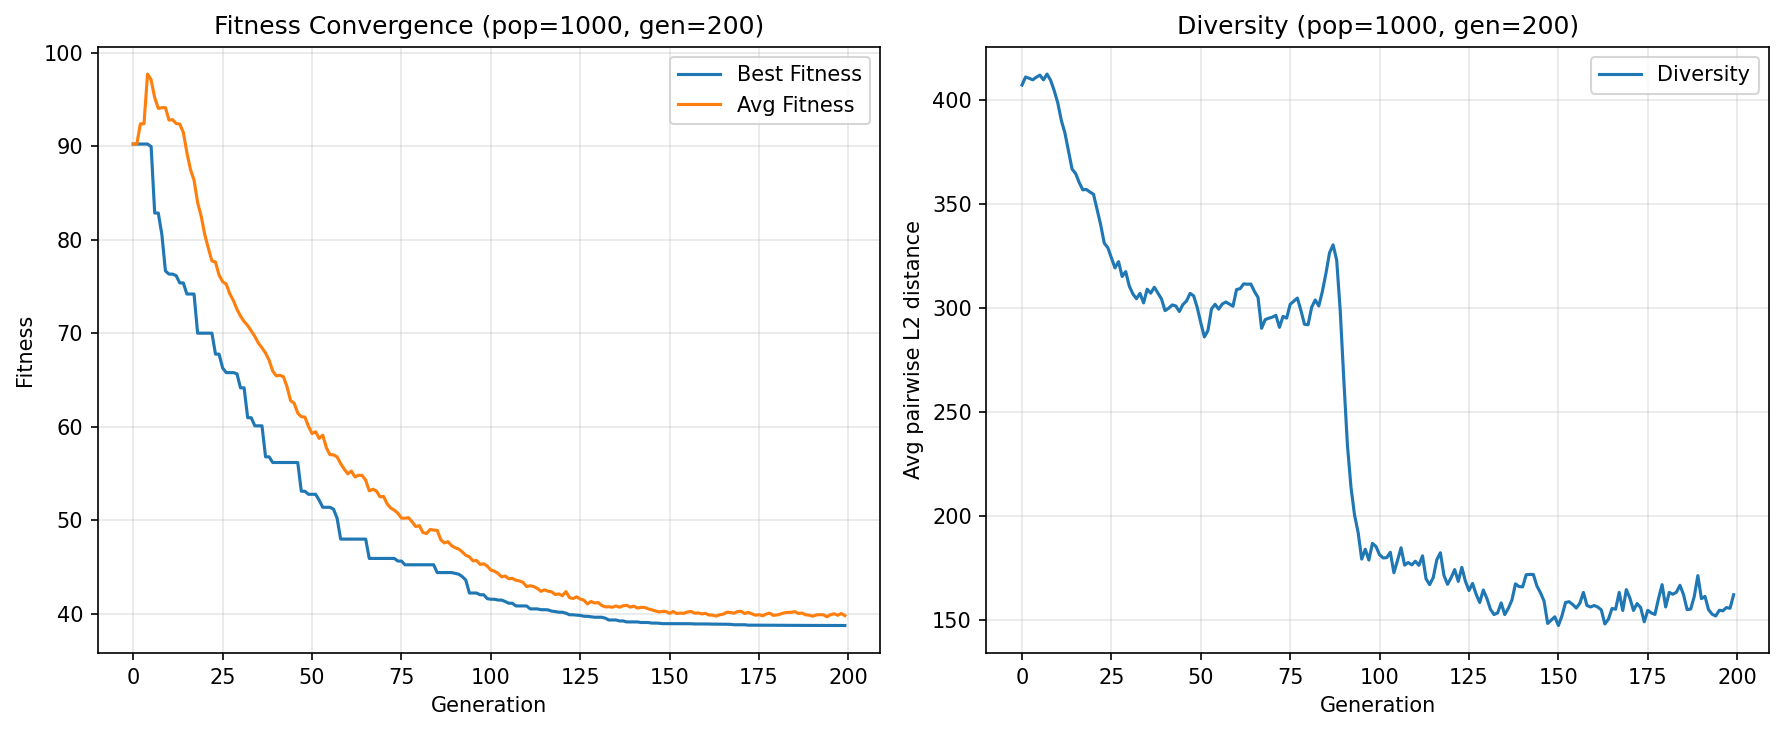
\includegraphics[width=0.9\linewidth]{ga_grid_results_incremental/pop_1000/pop_1000_gen_200.png}
    \caption{Fitness convergence and diversity plot for population size 1000 and 200 generations.}
\end{figure}

\begin{figure}[H]
    \centering
    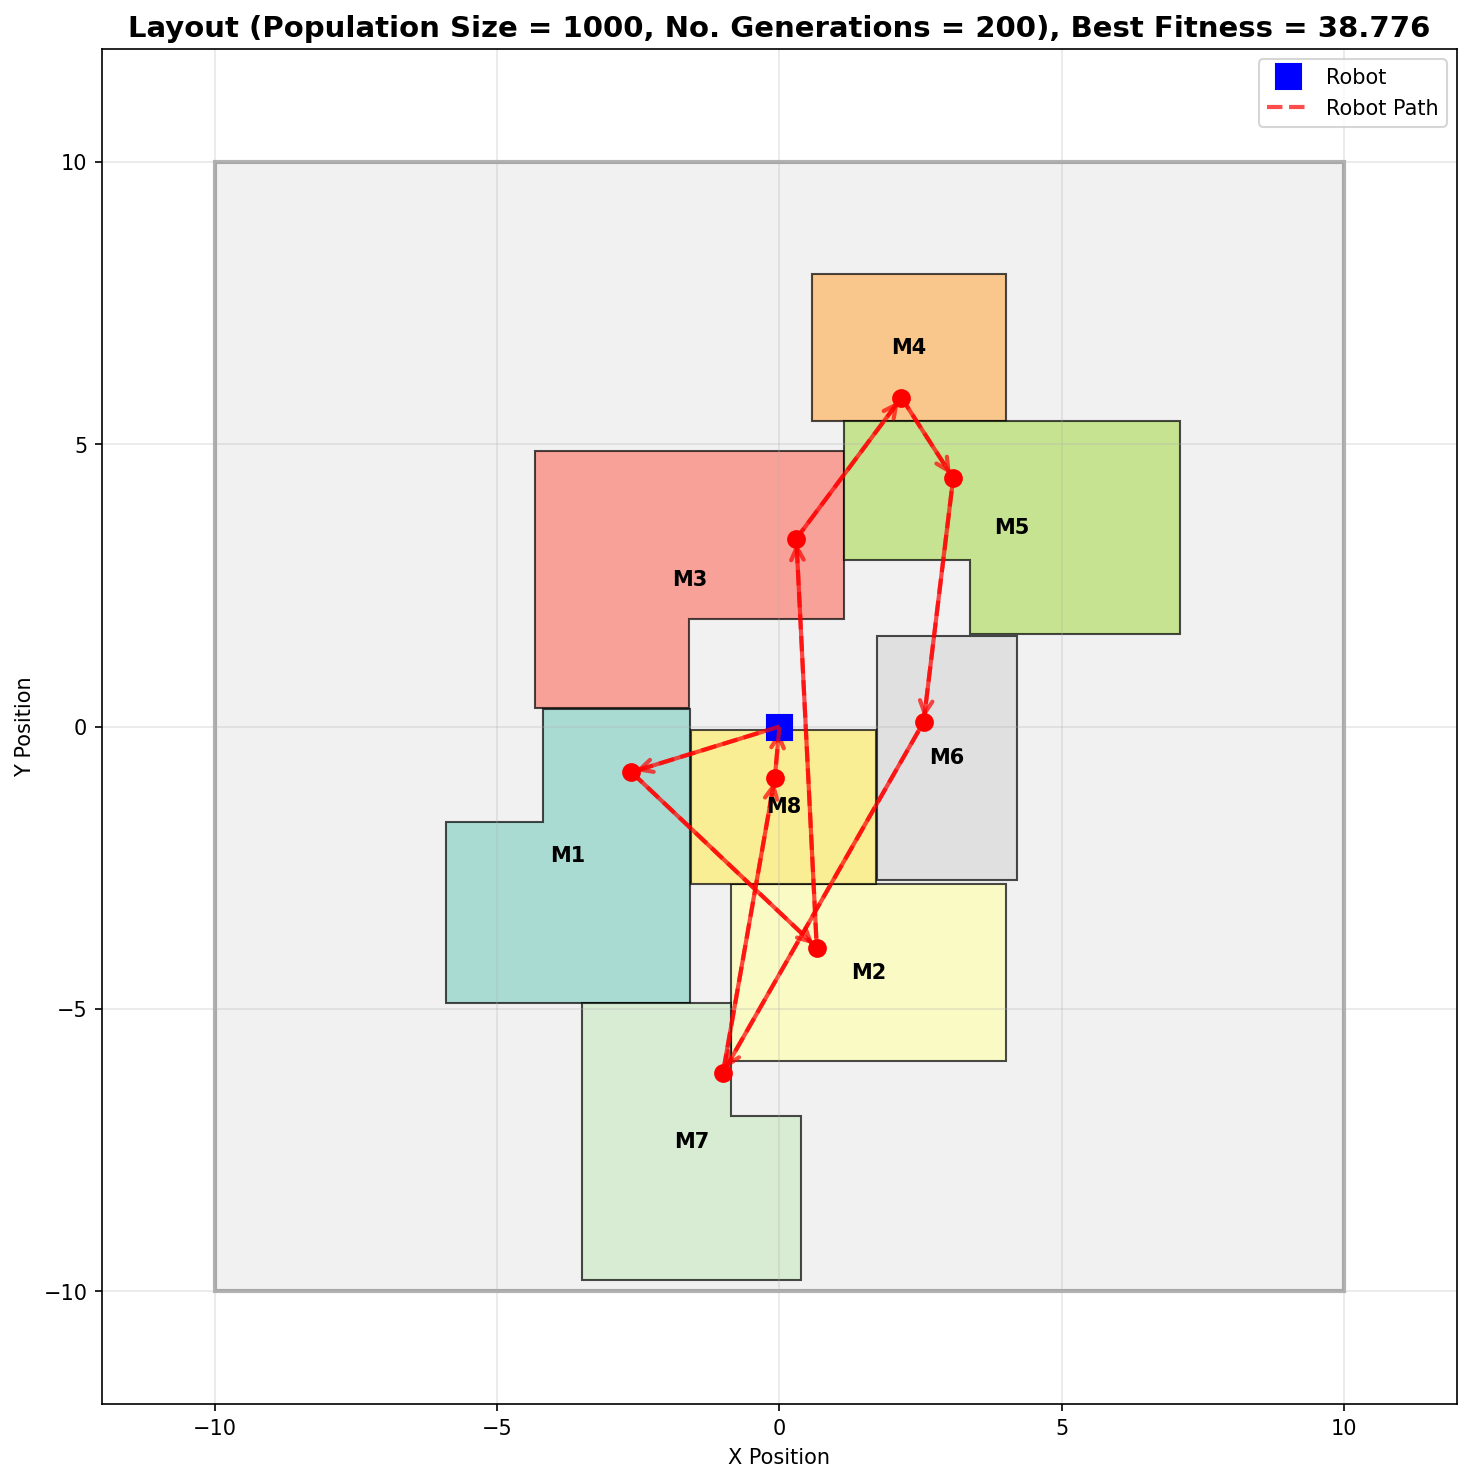
\includegraphics[width=0.7\linewidth]{ga_grid_results_incremental/pop_1000/layout_pop_1000_gen_200.png}
    \caption{Final optimized layout for population size 1000 and 200 generations.}
\end{figure}

\clearpage

\subsubsection{Generations = 500}
\begin{figure}[H]
    \centering
    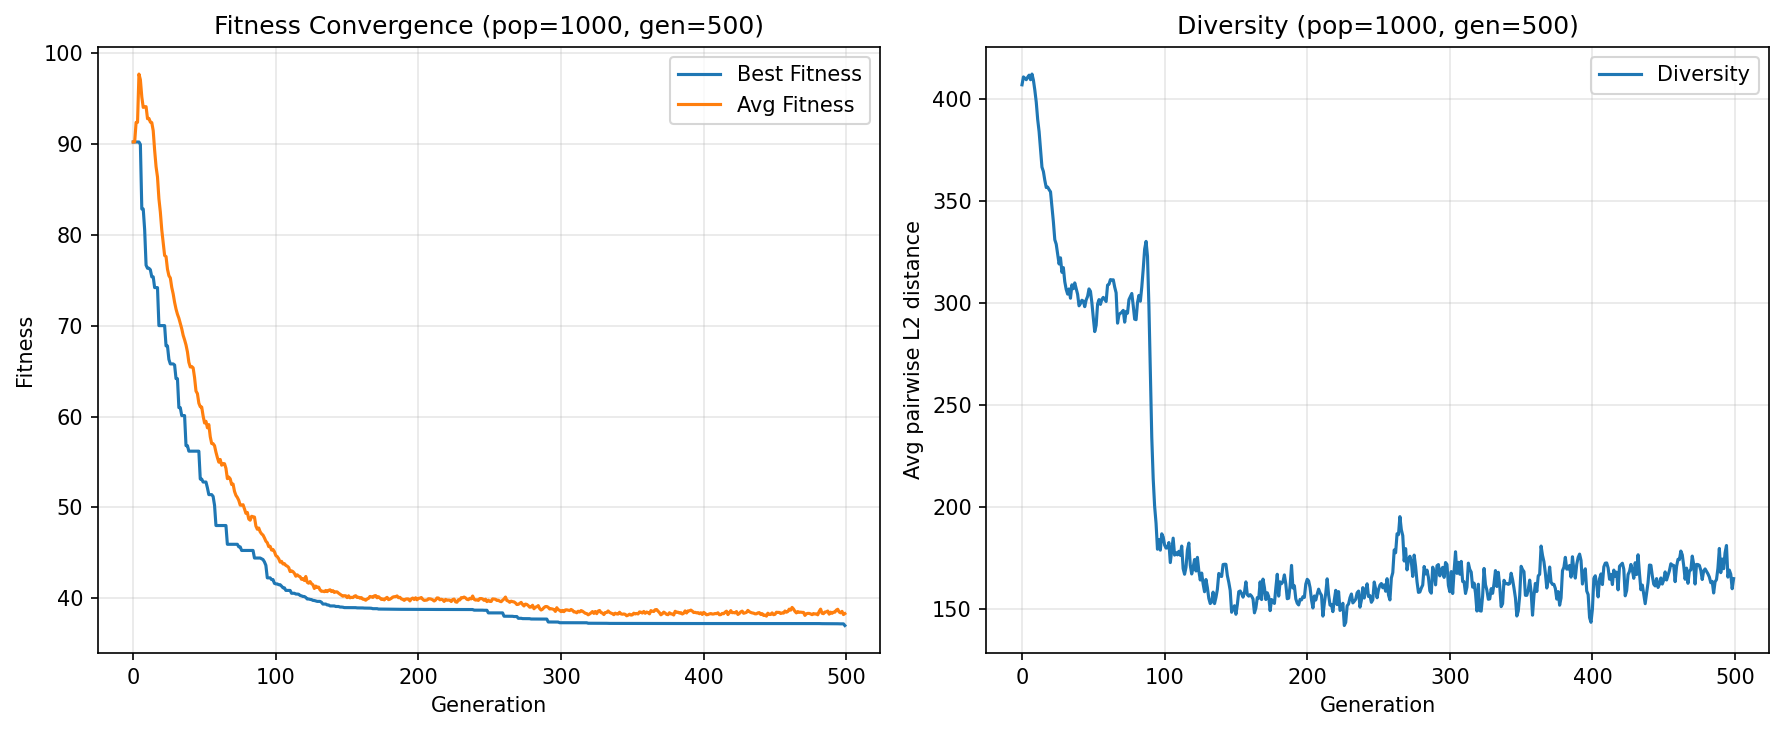
\includegraphics[width=0.9\linewidth]{ga_grid_results_incremental/pop_1000/pop_1000_gen_500.png}
    \caption{Fitness convergence and diversity plot for population size 1000 and 500 generations.}
\end{figure}

\begin{figure}[H]
    \centering
    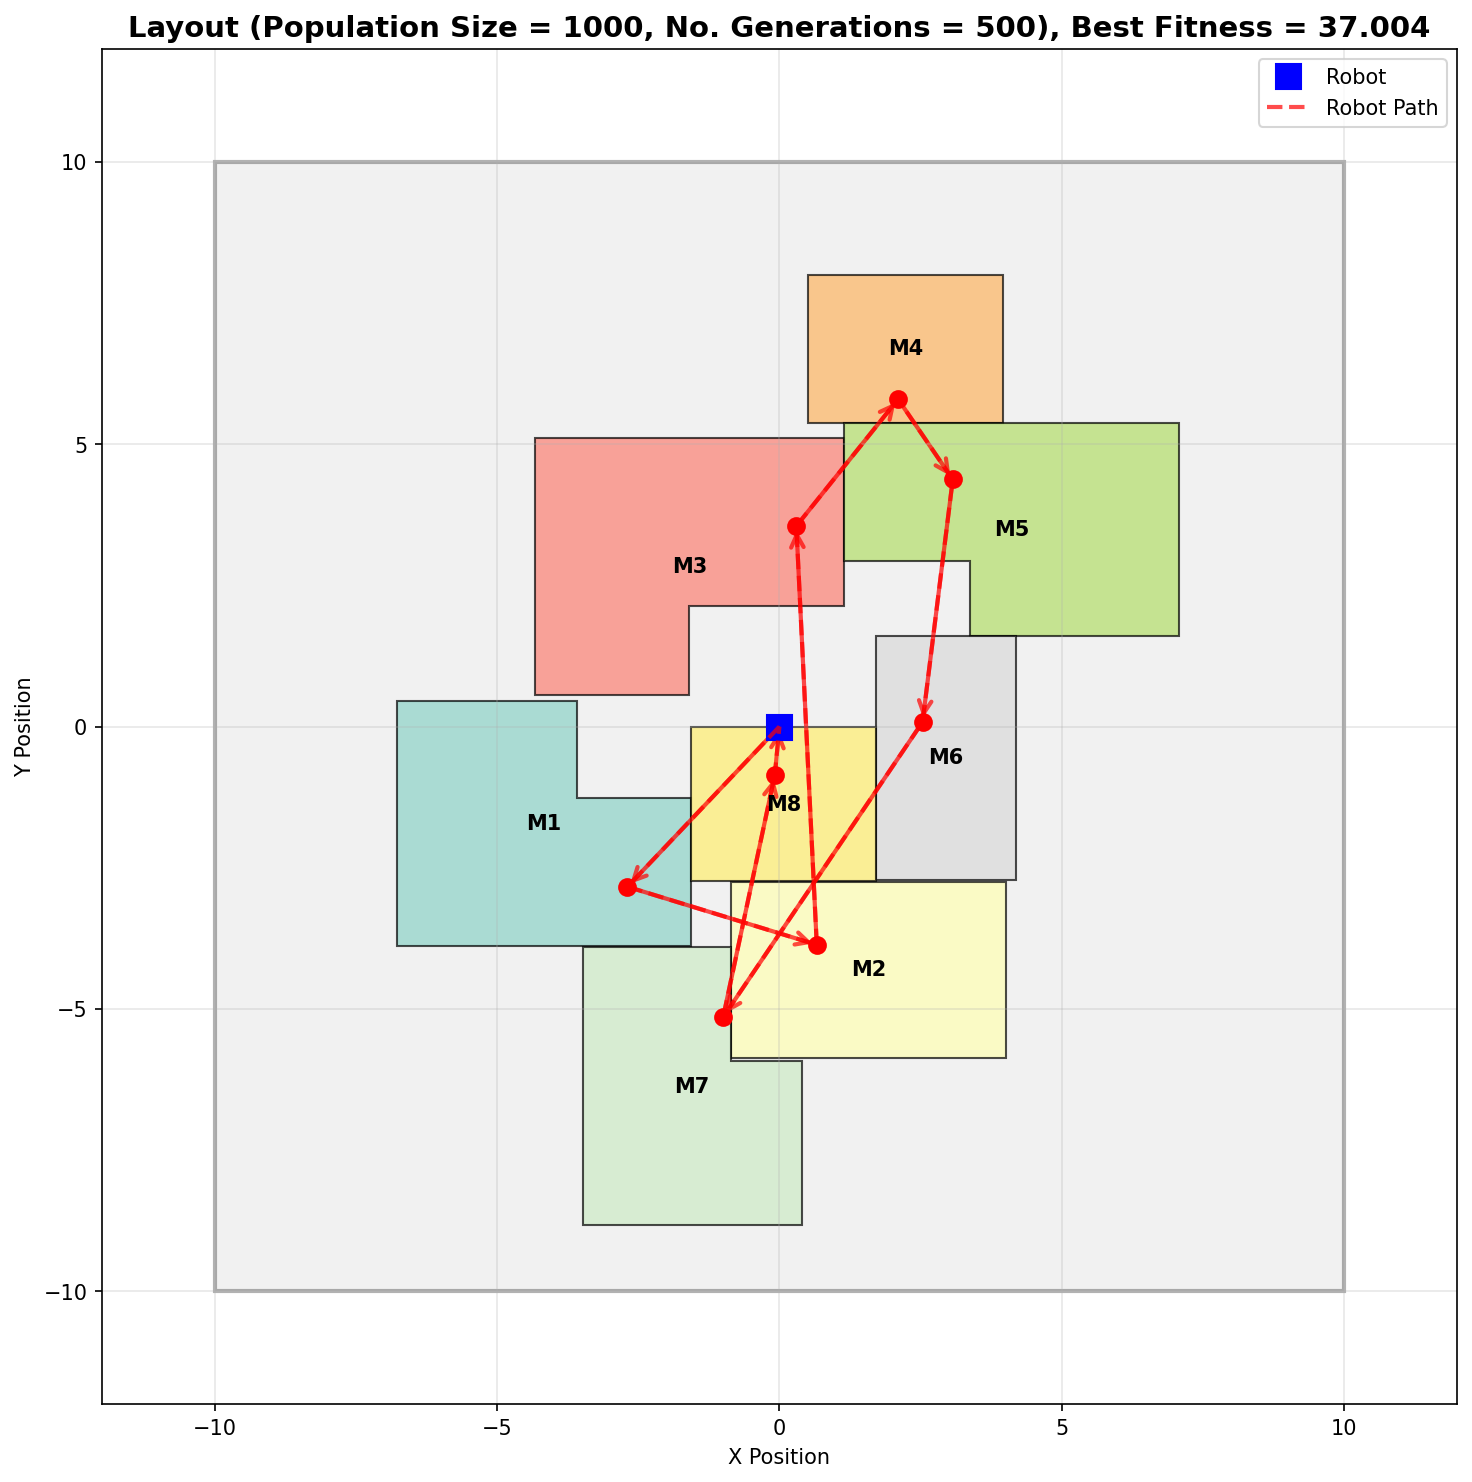
\includegraphics[width=0.7\linewidth]{ga_grid_results_incremental/pop_1000/layout_pop_1000_gen_500.png}
    \caption{Final optimized layout for population size 1000 and 500 generations.}
\end{figure}

\clearpage

\subsubsection{Generations = 1000}
\begin{figure}[H]
    \centering
    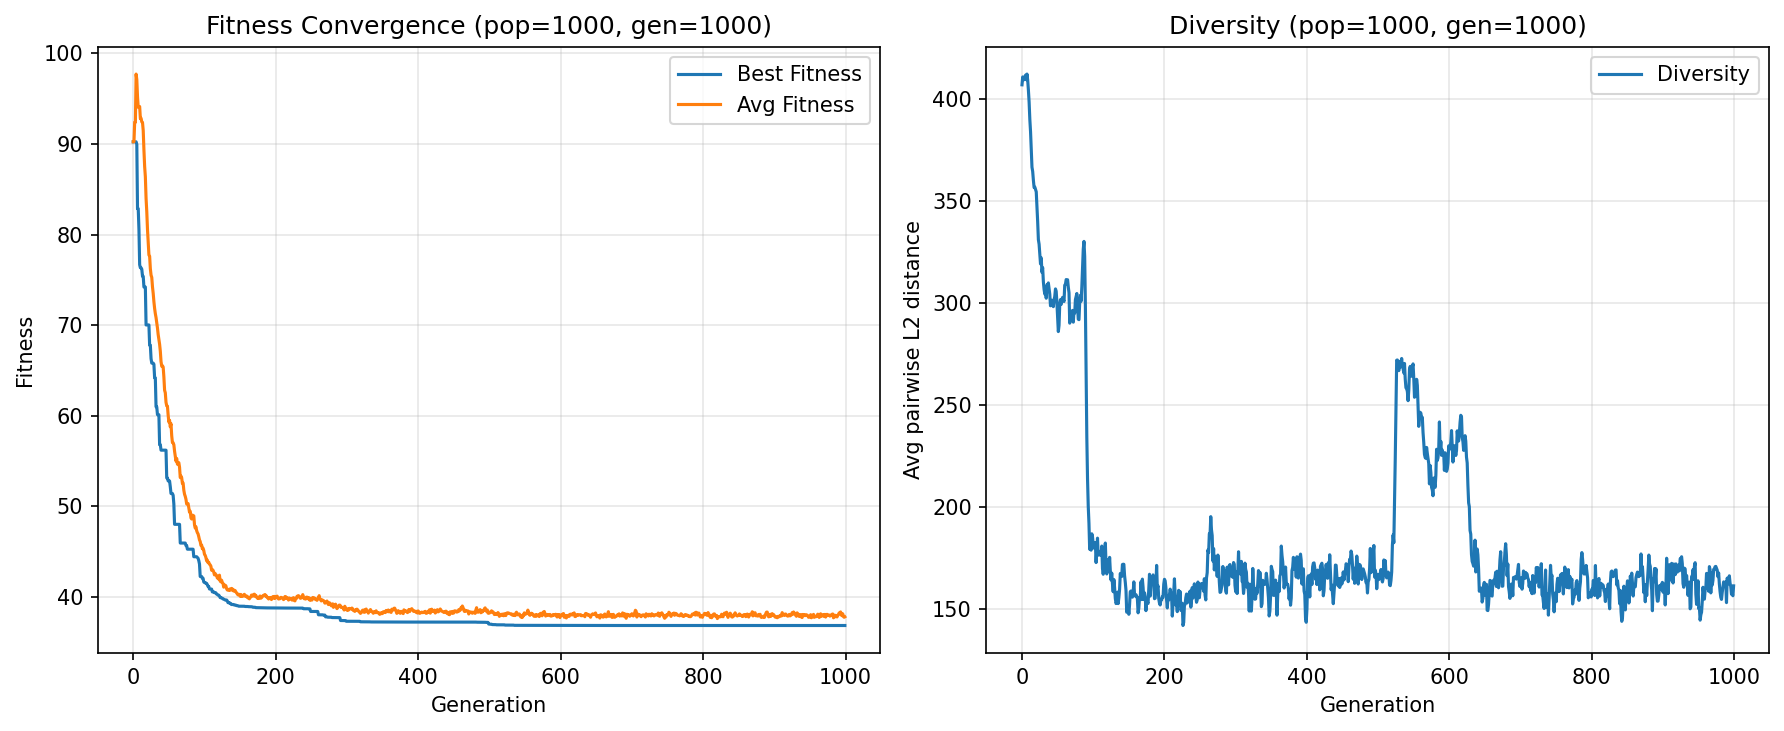
\includegraphics[width=0.9\linewidth]{ga_grid_results_incremental/pop_1000/pop_1000_gen_1000.png}
    \caption{Fitness convergence and diversity plot for population size 1000 and 1000 generations.}
\end{figure}

\begin{figure}[H]
    \centering
    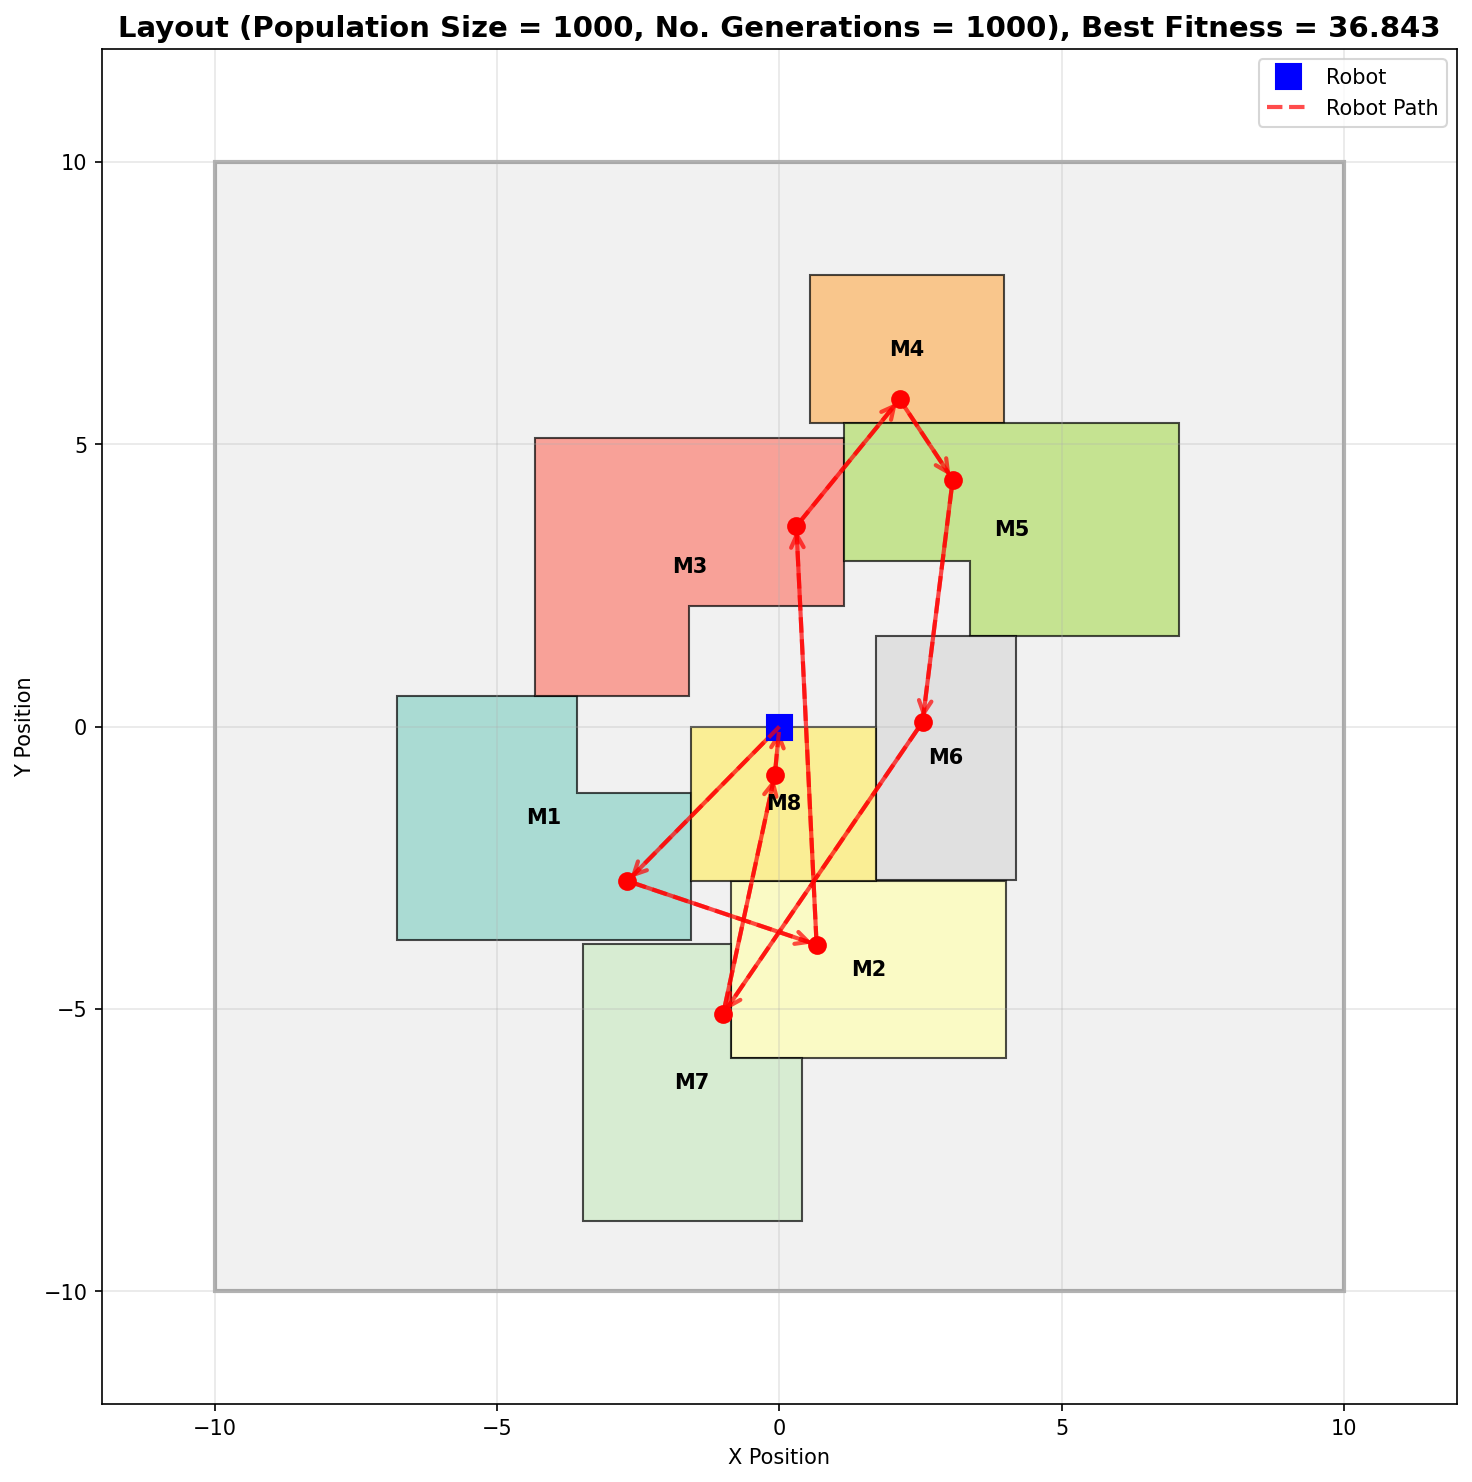
\includegraphics[width=0.7\linewidth]{ga_grid_results_incremental/pop_1000/layout_pop_1000_gen_1000.png}
    \caption{Final optimized layout for population size 1000 and 1000 generations.}
\end{figure}

\clearpage

\subsubsection{Generations = 2000}
\begin{figure}[H]
    \centering
    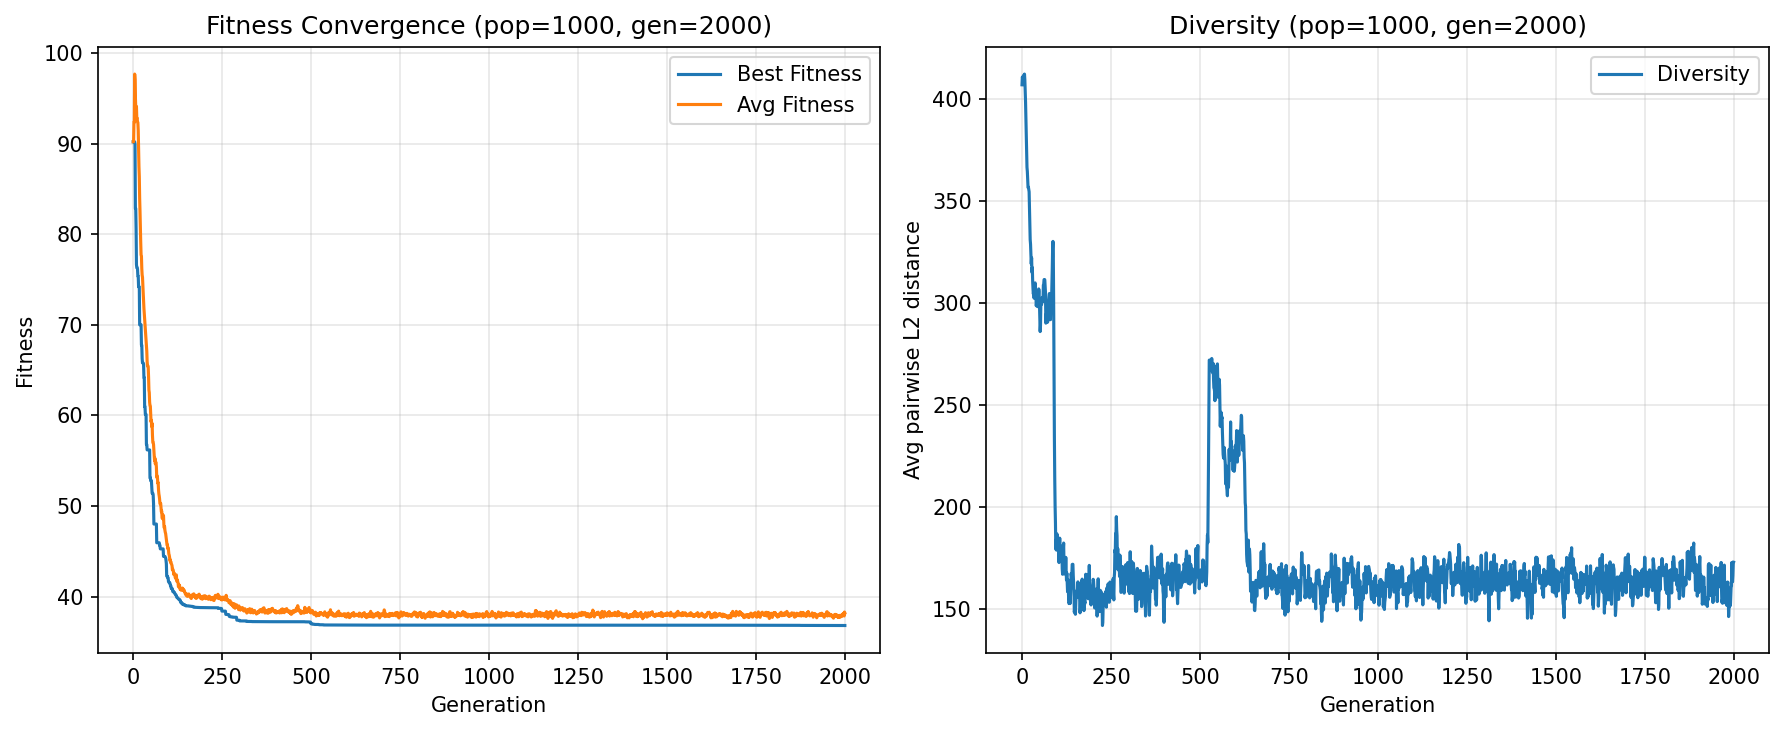
\includegraphics[width=0.9\linewidth]{ga_grid_results_incremental/pop_1000/pop_1000_gen_2000.png}
    \caption{Fitness convergence and diversity plot for population size 1000 and 2000 generations.}
\end{figure}

\begin{figure}[H]
    \centering
    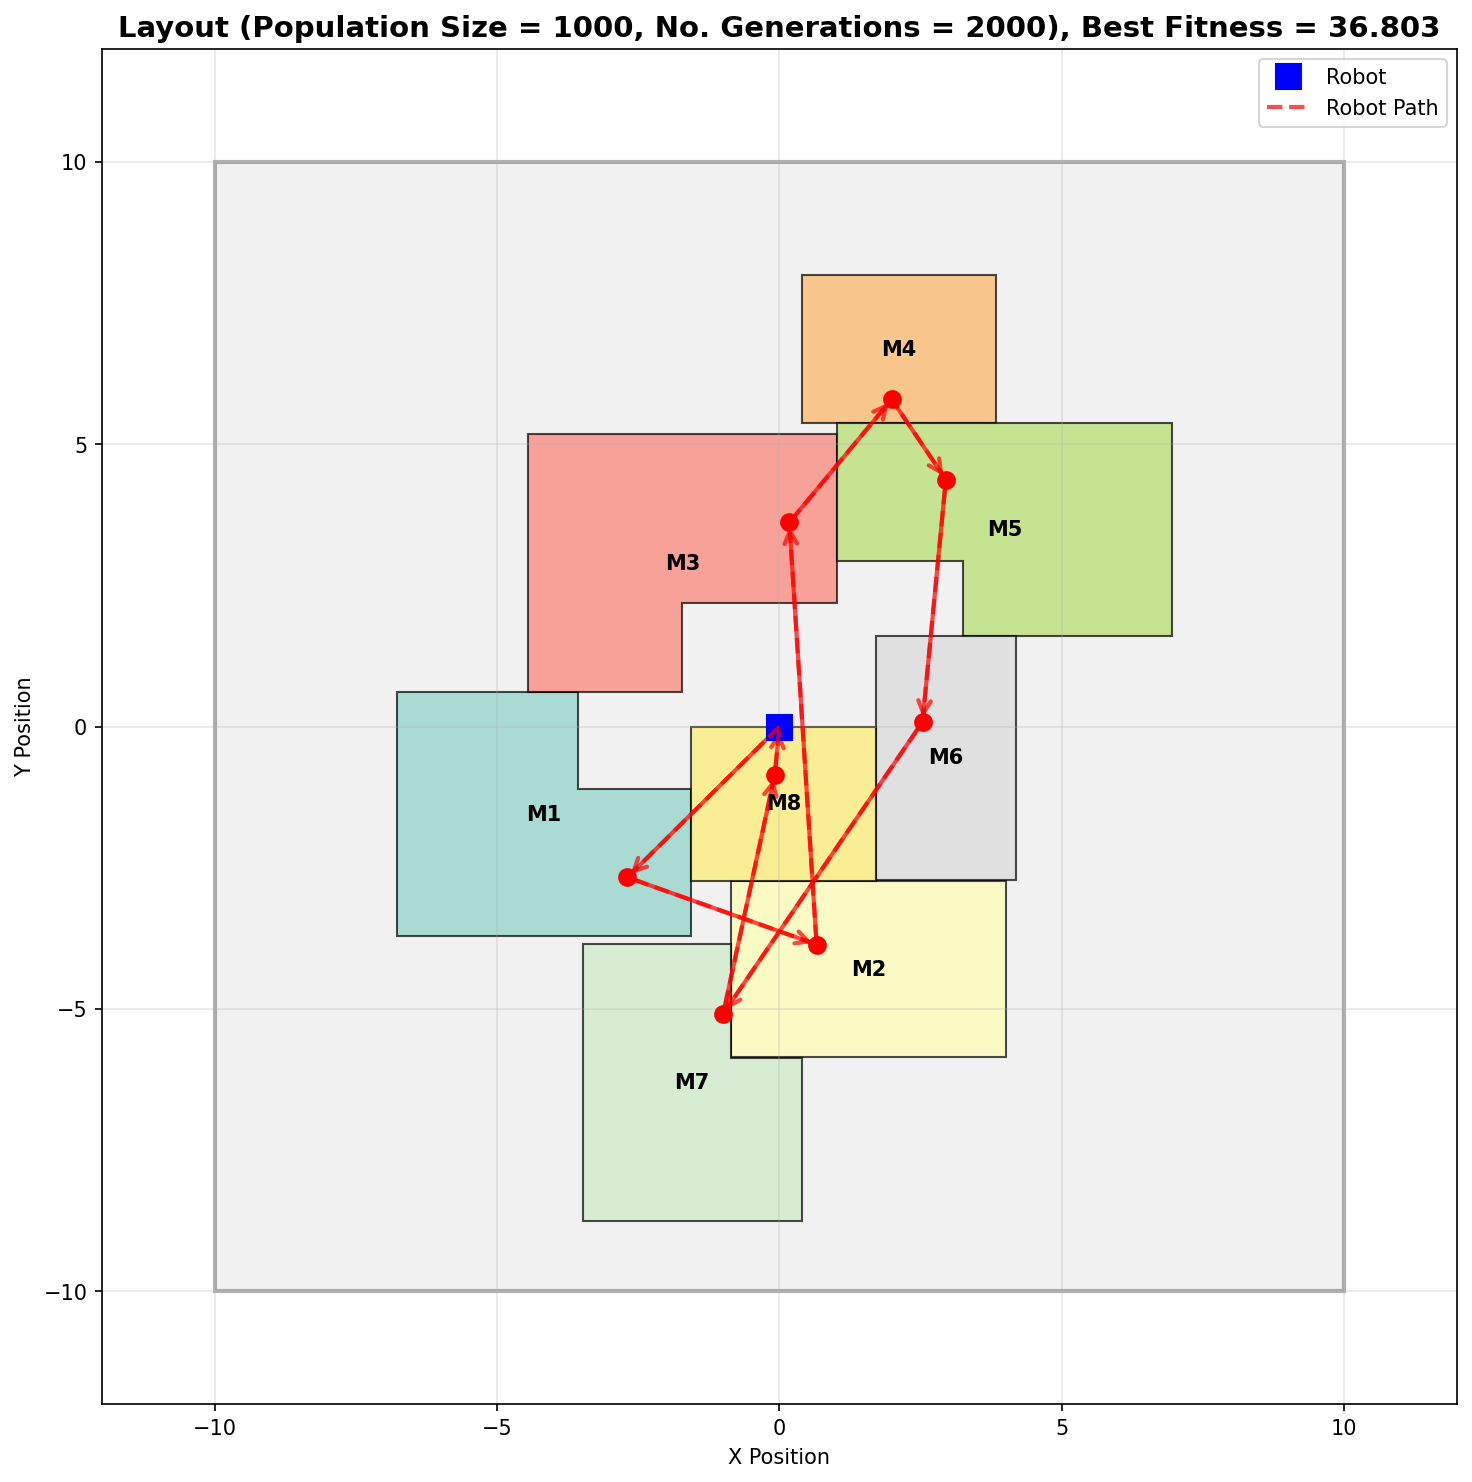
\includegraphics[width=0.7\linewidth]{ga_grid_results_incremental/pop_1000/layout_pop_1000_gen_2000.png}
    \caption{Final optimized layout for population size 1000 and 2000 generations.}
\end{figure}

\clearpage

%====================================================
\subsection{Population Size = 2000}
%====================================================

\subsubsection{Generations = 100}
\begin{figure}[H]
    \centering
    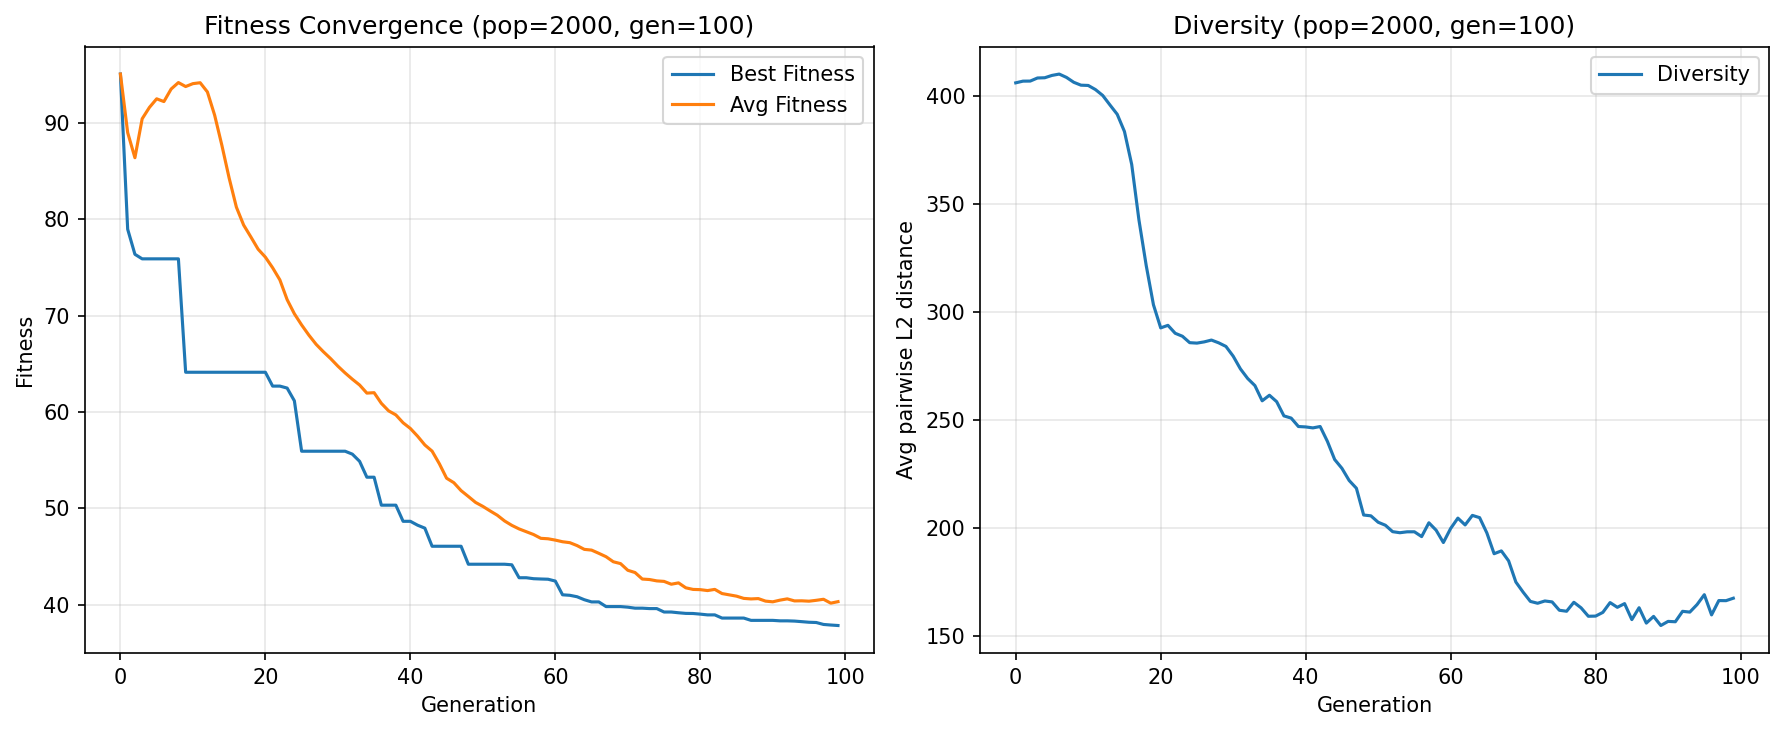
\includegraphics[width=0.9\linewidth]{ga_grid_results_incremental/pop_2000/pop_2000_gen_100.png}
    \caption{Fitness convergence and diversity plot for population size 2000 and 100 generations.}
\end{figure}

\begin{figure}[H]
    \centering
    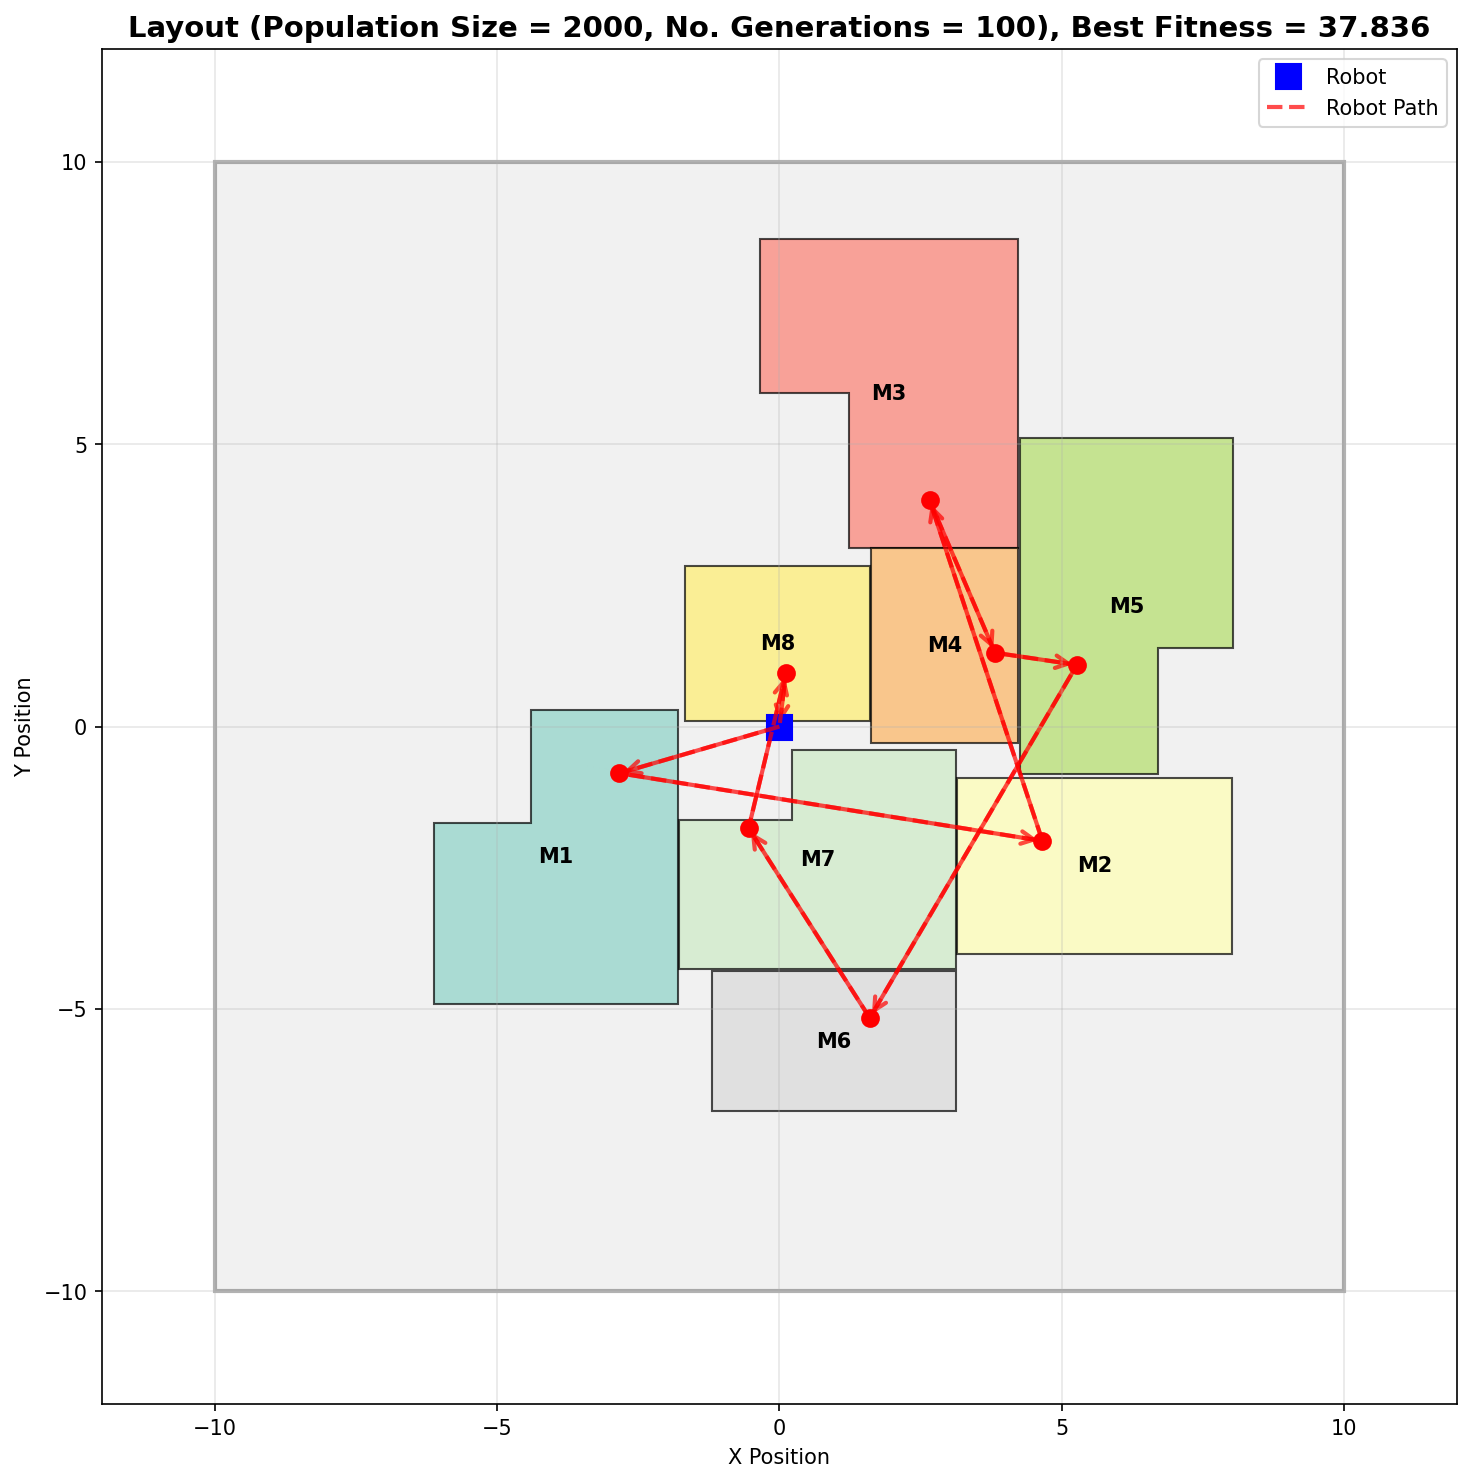
\includegraphics[width=0.7\linewidth]{ga_grid_results_incremental/pop_2000/layout_pop_2000_gen_100.png}
    \caption{Final optimized layout for population size 2000 and 100 generations.}
\end{figure}

\clearpage

\subsubsection{Generations = 200}
\begin{figure}[H]
    \centering
    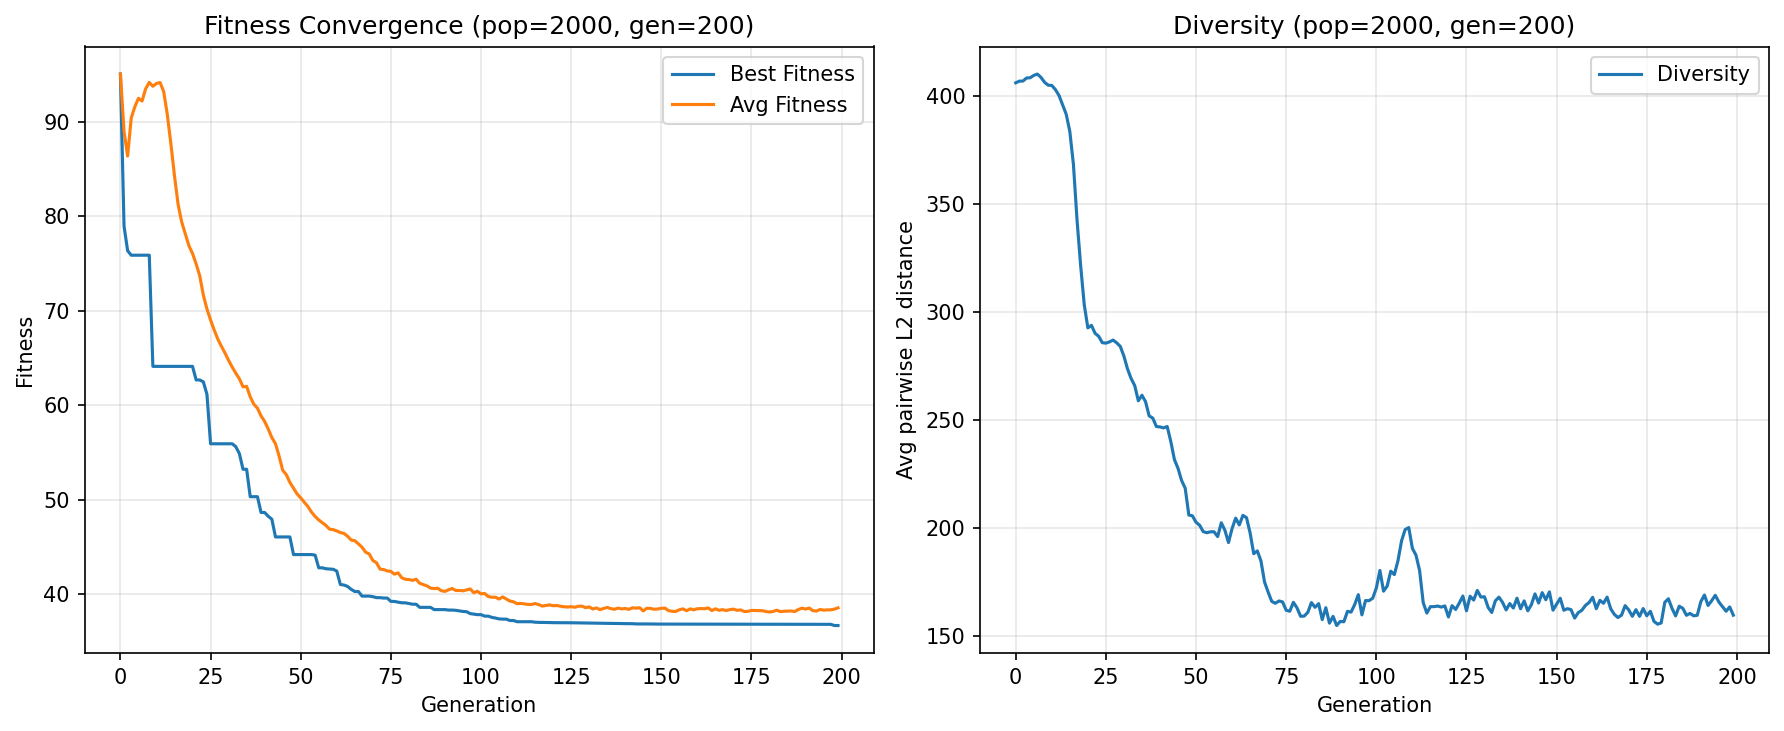
\includegraphics[width=0.9\linewidth]{ga_grid_results_incremental/pop_2000/pop_2000_gen_200.png}
    \caption{Fitness convergence and diversity plot for population size 2000 and 200 generations.}
\end{figure}

\begin{figure}[H]
    \centering
    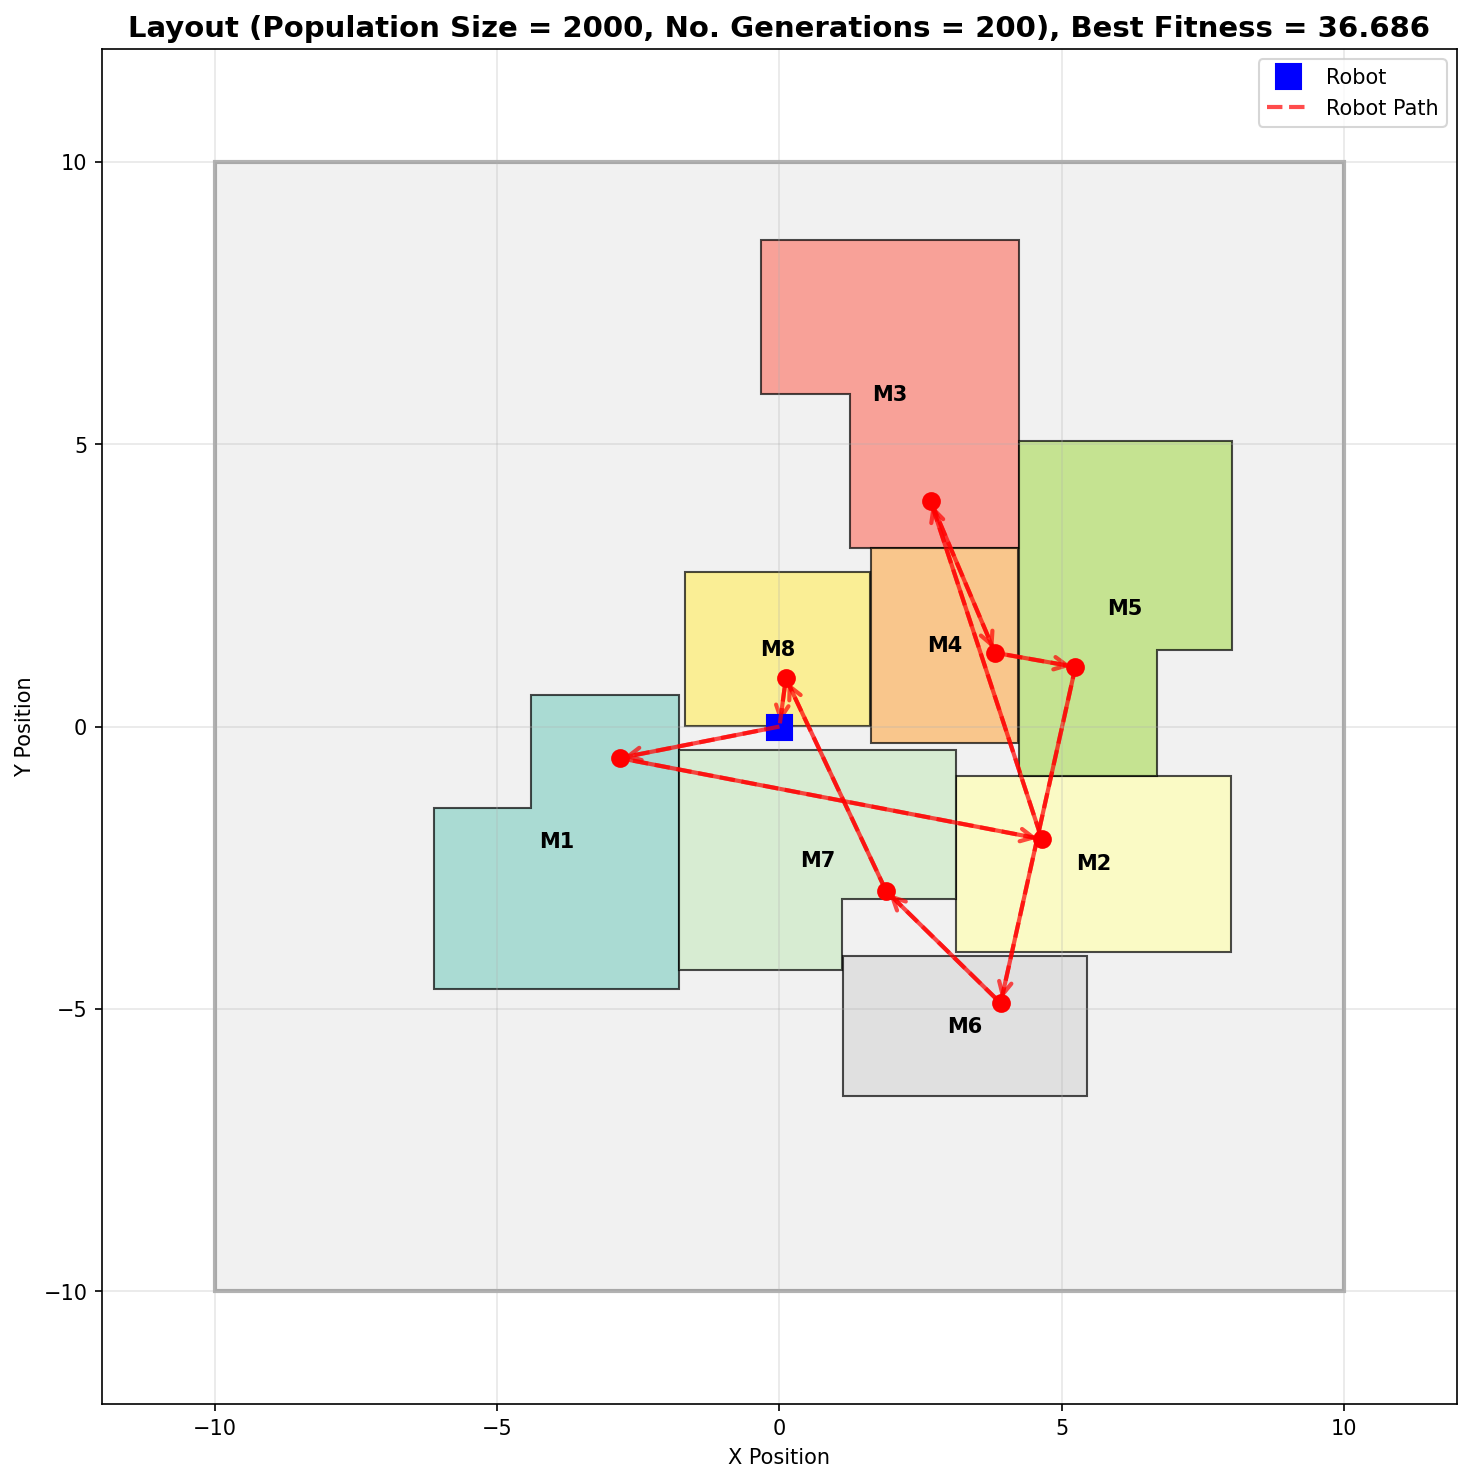
\includegraphics[width=0.7\linewidth]{ga_grid_results_incremental/pop_2000/layout_pop_2000_gen_200.png}
    \caption{Final optimized layout for population size 2000 and 200 generations.}
\end{figure}

\clearpage

\subsubsection{Generations = 500}
\begin{figure}[H]
    \centering
    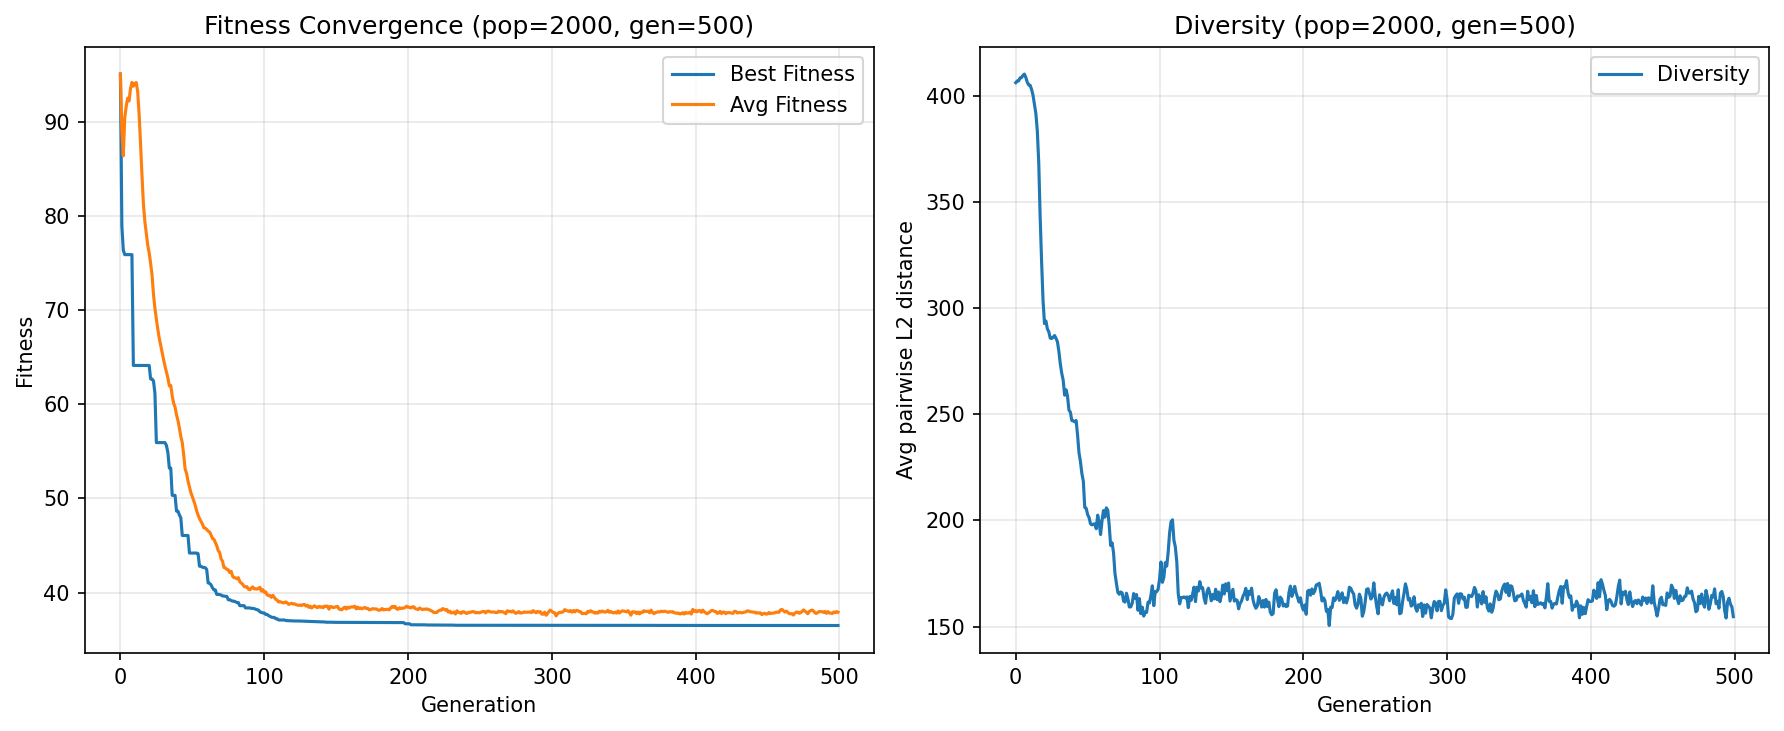
\includegraphics[width=0.9\linewidth]{ga_grid_results_incremental/pop_2000/pop_2000_gen_500.png}
    \caption{Fitness convergence and diversity plot for population size 2000 and 500 generations.}
\end{figure}

\begin{figure}[H]
    \centering
    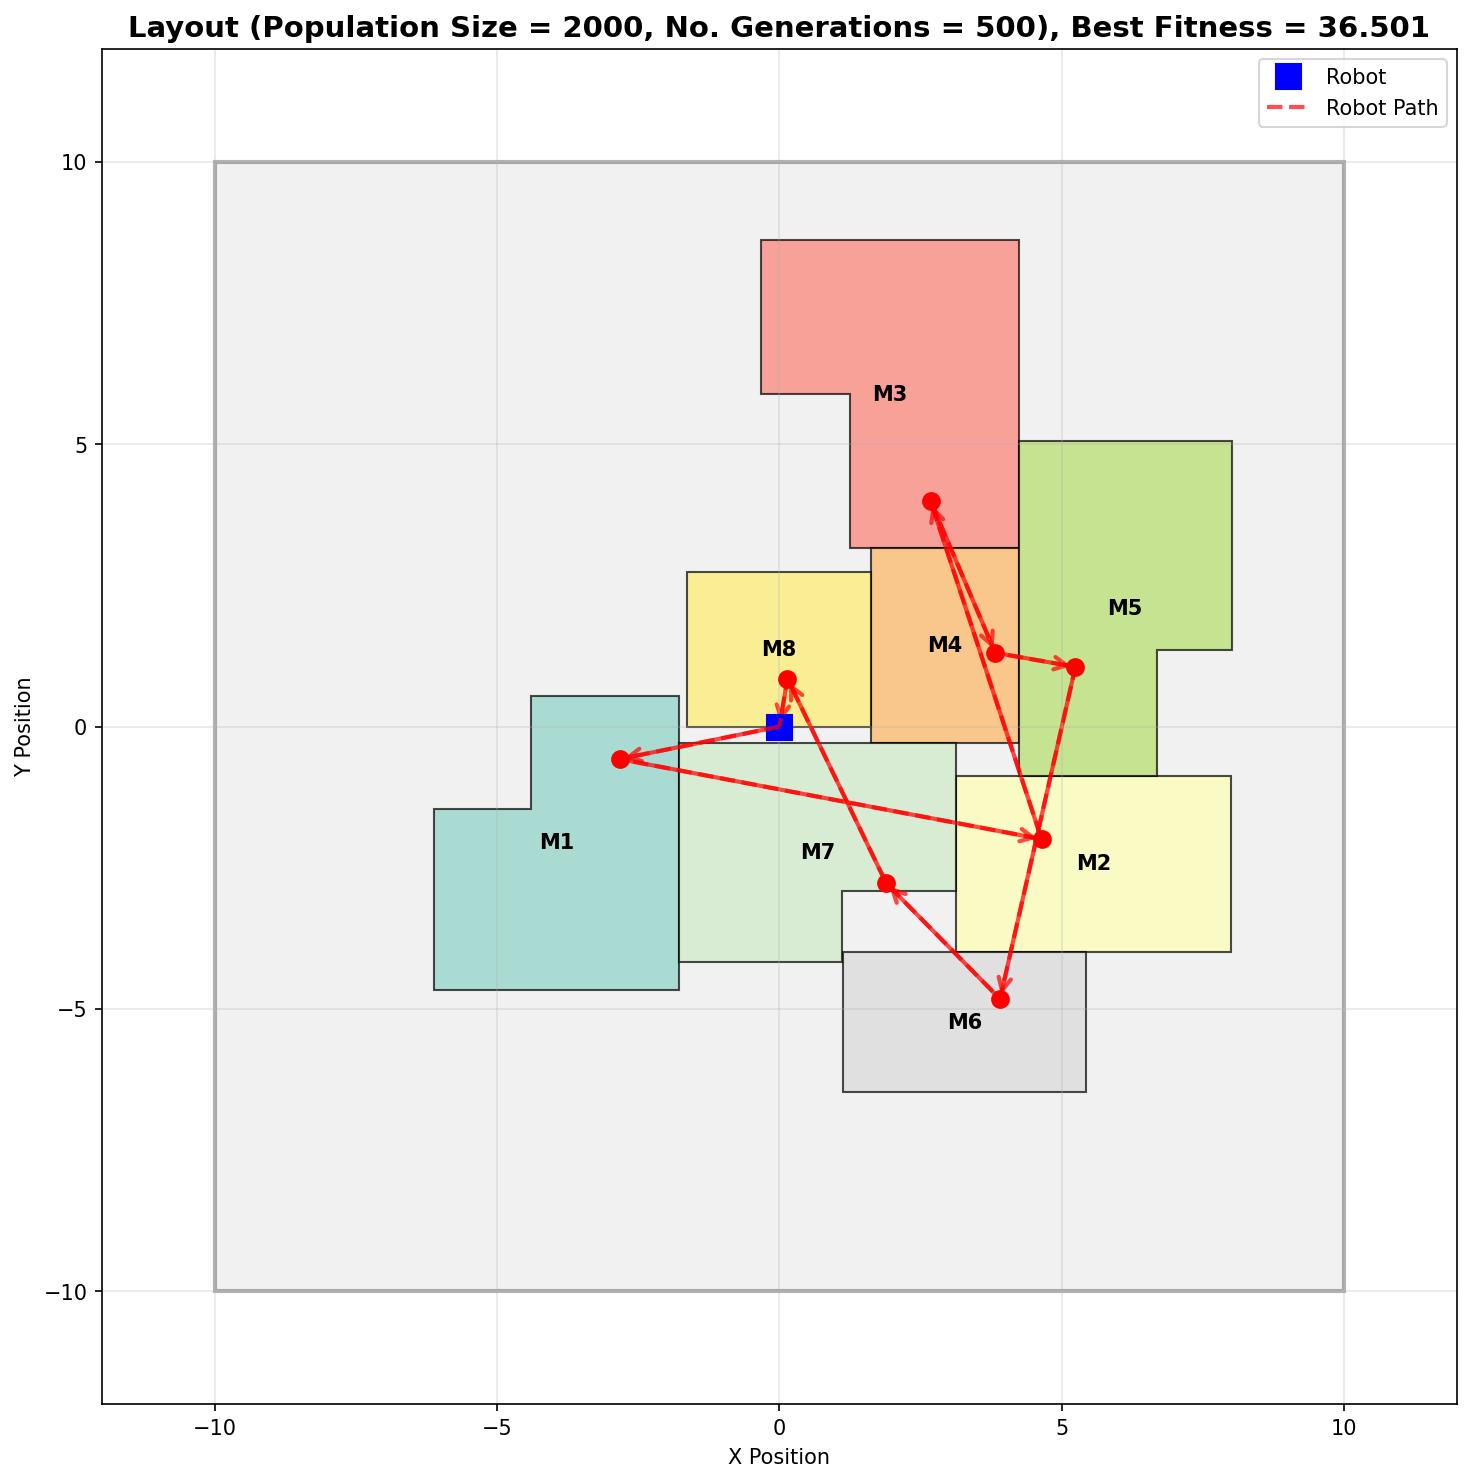
\includegraphics[width=0.7\linewidth]{ga_grid_results_incremental/pop_2000/layout_pop_2000_gen_500.png}
    \caption{Final optimized layout for population size 2000 and 500 generations.}
\end{figure}

\clearpage

\subsubsection{Generations = 1000}
\begin{figure}[H]
    \centering
    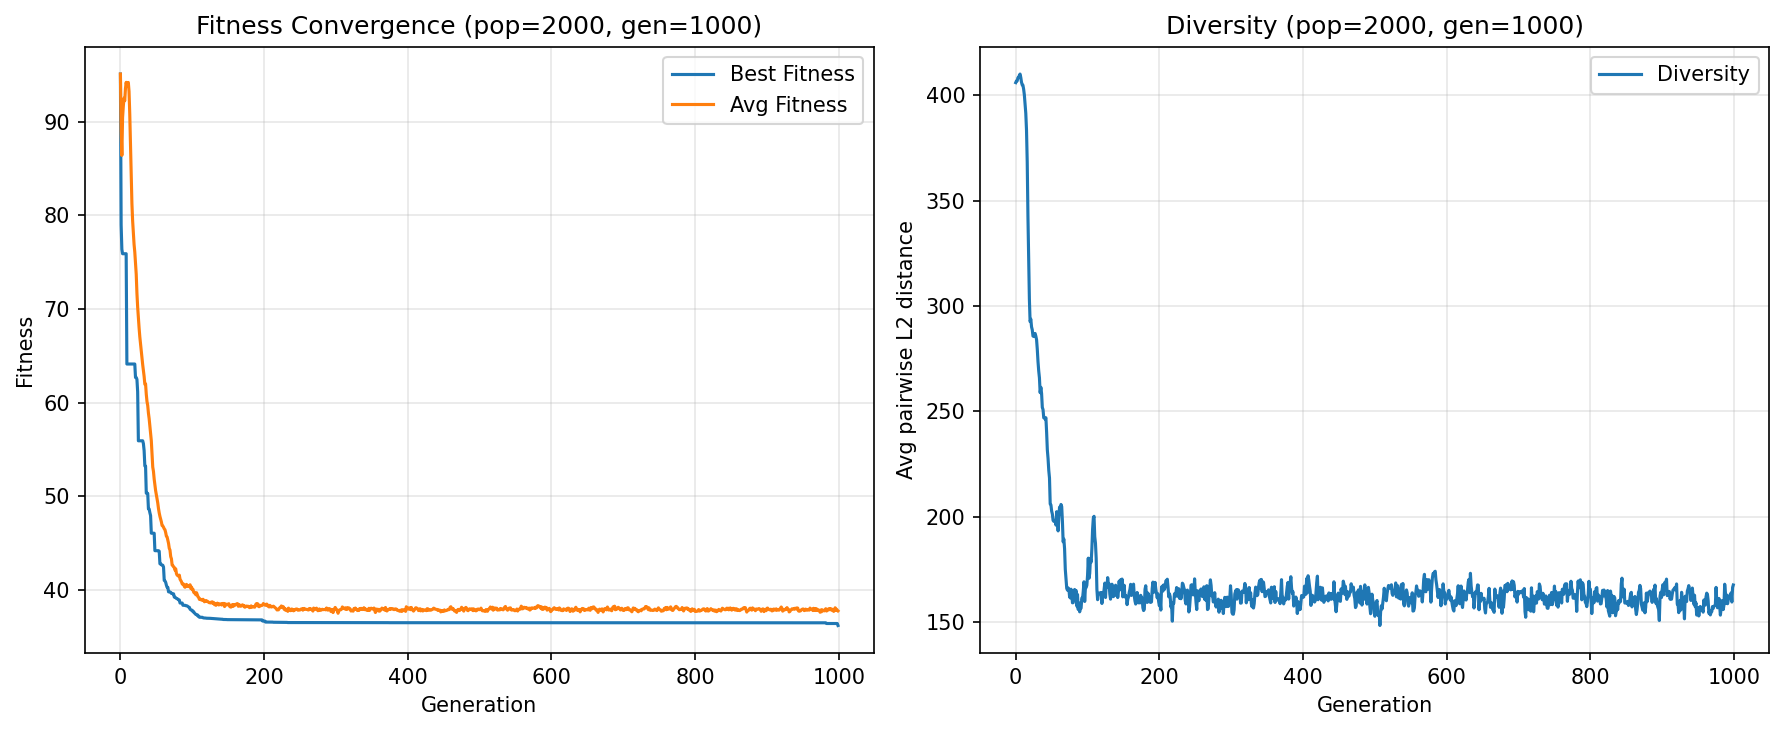
\includegraphics[width=0.9\linewidth]{ga_grid_results_incremental/pop_2000/pop_2000_gen_1000.png}
    \caption{Fitness convergence and diversity plot for population size 2000 and 1000 generations.}
\end{figure}

\begin{figure}[H]
    \centering
    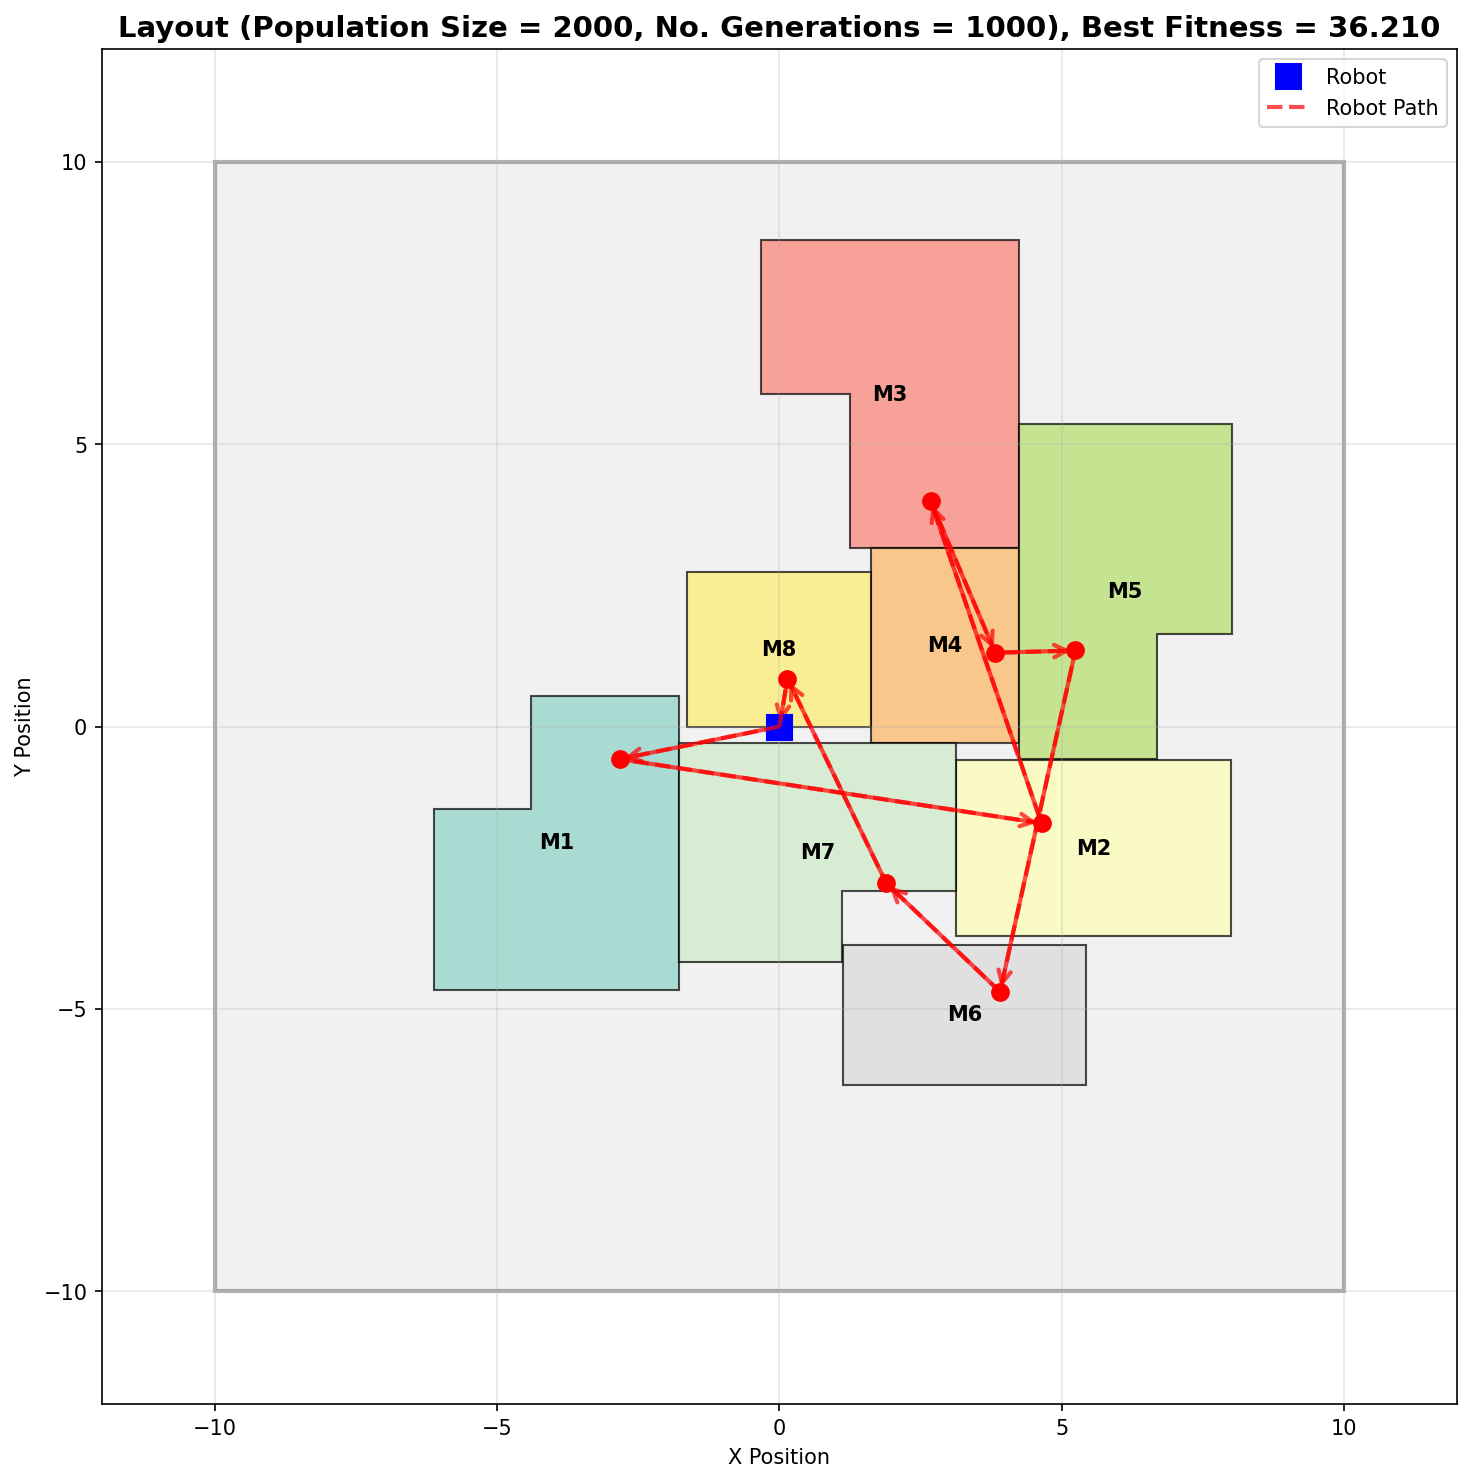
\includegraphics[width=0.7\linewidth]{ga_grid_results_incremental/pop_2000/layout_pop_2000_gen_1000.png}
    \caption{Final optimized layout for population size 2000 and 1000 generations.}
\end{figure}

\clearpage

\subsubsection{Generations = 2000}
\begin{figure}[H]
    \centering
    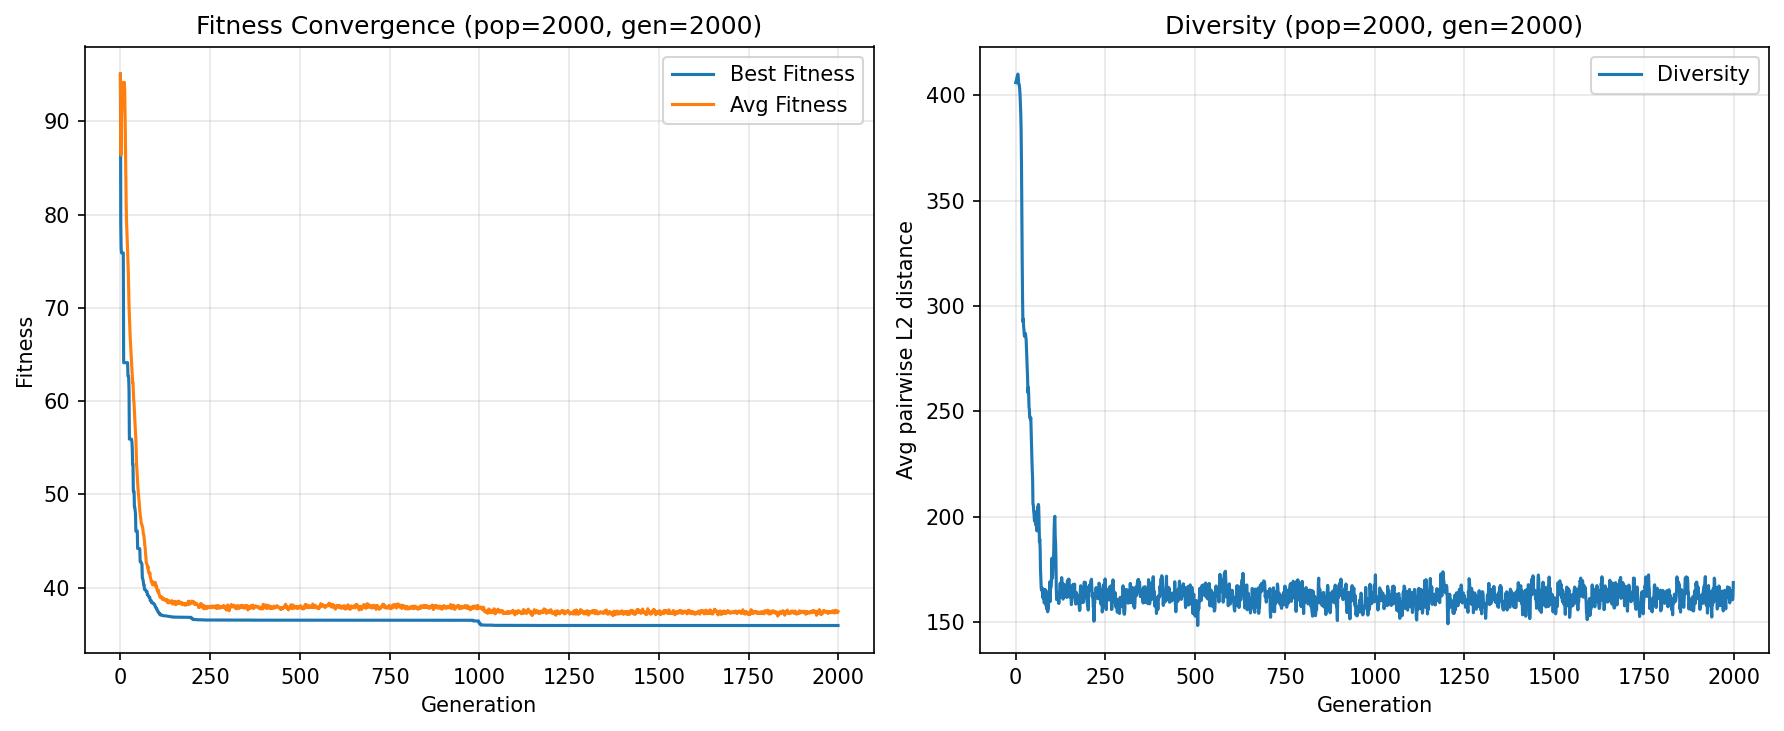
\includegraphics[width=0.9\linewidth]{ga_grid_results_incremental/pop_2000/pop_2000_gen_2000.png}
    \caption{Fitness convergence and diversity plot for population size 2000 and 2000 generations.}
\end{figure}

\begin{figure}[H]
    \centering
    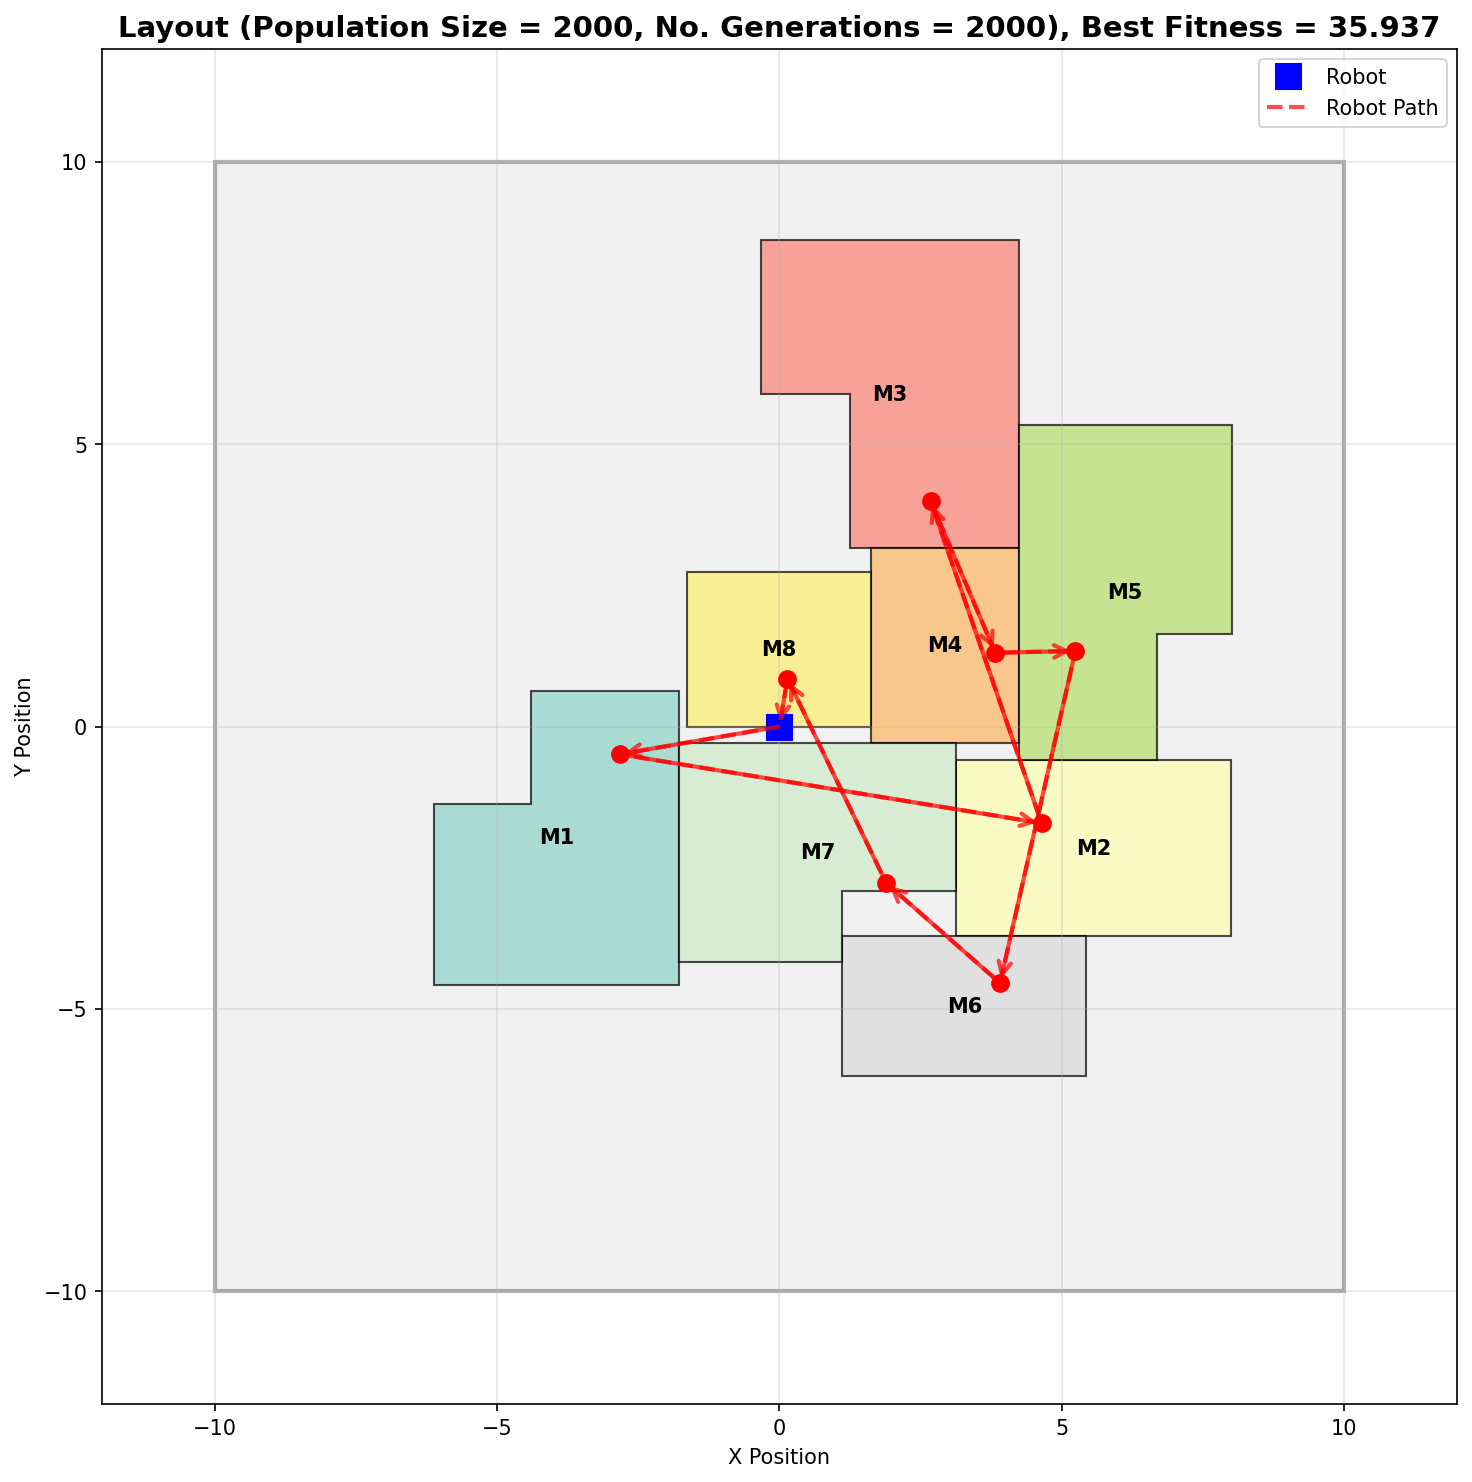
\includegraphics[width=0.7\linewidth]{ga_grid_results_incremental/pop_2000/layout_pop_2000_gen_2000.png}
    \caption{Final optimized layout for population size 2000 and 2000 generations.}
\end{figure}
%====================================================
\section{Appendix: RL Training Machine Definitions}
%====================================================

% ---------- Problem A ----------
\subsection{Problem A}
\begin{table}[H]
\centering
\small
\begin{tabular}{ccccccc}
\toprule
\textbf{ID} & \textbf{Shape} & \textbf{Width} & \textbf{Height} & \textbf{Access Point (x, y)} & \textbf{Cutout Width} & \textbf{Cutout Height} \\
\midrule
M1 & Rectangle & 4.0 & 3.0 & (1.5, 0.0)   & --   & --   \\
M2 & L-shape   & 5.0 & 4.0 & (-1.0, 1.0)  & 2.0  & 2.0  \\
M3 & Rectangle & 3.5 & 2.5 & (0.0, -1.0)  & --   & --   \\
M4 & L-shape   & 4.5 & 3.5 & (1.0, -0.5)  & 1.5  & 1.5  \\
M5 & L-shape   & 3.5 & 5.5 & (1.0, -1.0)  & 1.0  & 2.0  \\
M6 & L-shape   & 3.5 & 5.5 & (1.0, -1.0)  & 1.0  & 2.0  \\
M7 & L-shape   & 3.5 & 5.5 & (1.0, -1.0)  & 1.0  & 2.0  \\
M8 & Rectangle & 3.5 & 2.5 & (0.0, -1.0)  & --   & --   \\
\bottomrule
\end{tabular}
\caption{Machine Configuration for Problem A}
\label{tab:machine_config_a}
\end{table}

% ---------- Problem B ----------
\subsection{Problem B}
\begin{table}[H]
\centering
\small
\begin{tabular}{ccccccc}
\toprule
\textbf{ID} & \textbf{Shape} & \textbf{Width} & \textbf{Height} & \textbf{Access Point (x, y)} & \textbf{Cutout Width} & \textbf{Cutout Height} \\
\midrule
M1 & Rectangle & 4.0 & 3.0 & (1.5, 0.0)   & --   & --   \\
M2 & L-shape   & 5.0 & 4.0 & (-1.0, 1.0)  & 2.0  & 2.0  \\
M3 & Rectangle & 3.5 & 2.5 & (0.0, -1.0)  & --   & --   \\
M4 & L-shape   & 4.5 & 3.5 & (1.0, -0.5)  & 1.5  & 1.5  \\
M5 & L-shape   & 3.0 & 5.5 & (1.0, -1.0)  & 1.0  & 2.0  \\
M6 & L-shape   & 5.0 & 3.0 & (1.0, -1.0)  & 2.0  & 2.0  \\
M7 & L-shape   & 3.5 & 2.5 & (1.0, -1.0)  & 1.0  & 2.0  \\
M8 & Rectangle & 3.5 & 2.5 & (0.0, 0.0)   & --   & --   \\
\bottomrule
\end{tabular}
\caption{Machine Configuration for Problem B}
\label{tab:machine_config_b}
\end{table}

% ---------- Problem C ----------
\subsection{Problem C}
\begin{table}[H]
\centering
\small
\begin{tabular}{ccccccc}
\toprule
\textbf{ID} & \textbf{Shape} & \textbf{Width} & \textbf{Height} & \textbf{Access Point (x, y)} & \textbf{Cutout Width} & \textbf{Cutout Height} \\
\midrule
M1 & Rectangle & 6.0 & 3.0 & (2.0, 0.0)   & -- & -- \\
M2 & Rectangle & 5.5 & 2.5 & (-1.0, 0.0)  & -- & -- \\
M3 & Rectangle & 4.5 & 3.0 & (0.0, -1.0)  & -- & -- \\
M4 & Rectangle & 3.5 & 4.0 & (0.0, 1.5)   & -- & -- \\
M5 & Rectangle & 4.0 & 4.0 & (1.0, -1.0)  & -- & -- \\
M6 & Rectangle & 5.0 & 3.5 & (-1.5, 0.0)  & -- & -- \\
M7 & Rectangle & 6.0 & 2.5 & (0.0, 1.0)   & -- & -- \\
M8 & Rectangle & 4.0 & 2.0 & (0.5, 0.0)   & -- & -- \\
\bottomrule
\end{tabular}
\caption{Machine Configuration for Problem C}
\label{tab:machine_config_c}
\end{table}

% ---------- Problem D ----------
\subsection{Problem D}
\begin{table}[H]
\centering
\small
\begin{tabular}{ccccccc}
\toprule
\textbf{ID} & \textbf{Shape} & \textbf{Width} & \textbf{Height} & \textbf{Access Point (x, y)} & \textbf{Cutout Width} & \textbf{Cutout Height} \\
\midrule
M1 & Rectangle & 2.5 & 2.5 & (0.5, 0.0)   & --   & --   \\
M2 & L-shape   & 3.0 & 3.0 & (1.0, -0.5)  & 1.0  & 1.0  \\
M3 & Rectangle & 2.0 & 2.0 & (0.0, 1.0)   & --   & --   \\
M4 & L-shape   & 3.5 & 3.5 & (-0.5, 1.0)  & 1.0  & 1.2  \\
M5 & Rectangle & 2.0 & 3.0 & (0.5, -1.0)  & --   & --   \\
M6 & Rectangle & 3.0 & 2.0 & (1.0, 0.0)   & --   & --   \\
M7 & L-shape   & 3.0 & 3.5 & (1.0, 1.0)   & 1.0  & 1.0  \\
M8 & Rectangle & 2.5 & 2.0 & (0.0, 0.0)   & --   & --   \\
\bottomrule
\end{tabular}
\caption{Machine Configuration for Problem D}
\label{tab:machine_config_d}
\end{table}

% ---------- Problem E ----------
\subsection{Problem E}
\begin{table}[H]
\centering
\small
\begin{tabular}{ccccccc}
\toprule
\textbf{ID} & \textbf{Shape} & \textbf{Width} & \textbf{Height} & \textbf{Access Point (x, y)} & \textbf{Cutout Width} & \textbf{Cutout Height} \\
\midrule
M1 & L-shape   & 6.0 & 6.0 & (1.0, -1.0)  & 2.0  & 2.0  \\
M2 & L-shape   & 5.5 & 5.0 & (-1.0, 1.0)  & 2.0  & 2.0  \\
M3 & Rectangle & 6.0 & 4.0 & (0.0, -1.5)  & --   & --   \\
M4 & L-shape   & 6.5 & 5.5 & (1.0, 1.0)   & 2.5  & 2.0  \\
M5 & Rectangle & 5.0 & 5.0 & (1.5, 0.0)   & --   & --   \\
M6 & L-shape   & 5.0 & 4.5 & (0.0, -1.0)  & 1.5  & 1.5  \\
M7 & Rectangle & 5.5 & 4.0 & (-1.0, 0.0)  & --   & --   \\
M8 & Rectangle & 4.5 & 3.5 & (1.0, 0.0)   & --   & --   \\
\bottomrule
\end{tabular}
\caption{Machine Configuration for Problem E}
\label{tab:machine_config_e}
\end{table}

% ---------- Problem F ----------
\subsection{Problem F}
\begin{table}[H]
\centering
\small
\begin{tabular}{ccccccc}
\toprule
\textbf{ID} & \textbf{Shape} & \textbf{Width} & \textbf{Height} & \textbf{Access Point (x, y)} & \textbf{Cutout Width} & \textbf{Cutout Height} \\
\midrule
M1 & Rectangle & 2.0 & 6.0 & (0.8, 0.0)   & --   & --   \\
M2 & Rectangle & 2.5 & 5.5 & (-0.5, 1.0)  & --   & --   \\
M3 & L-shape   & 3.0 & 6.0 & (0.0, -1.0)  & 1.0  & 2.0  \\
M4 & Rectangle & 2.2 & 6.5 & (1.0, 0.0)   & --   & --   \\
M5 & Rectangle & 1.8 & 5.0 & (1.0, -1.0)  & --   & --   \\
M6 & L-shape   & 3.0 & 5.5 & (-1.0, 1.0)  & 1.0  & 1.5  \\
M7 & Rectangle & 2.5 & 6.0 & (0.0, 1.0)   & --   & --   \\
M8 & L-shape   & 3.5 & 5.0 & (0.5, 0.0)   & 1.0  & 2.0  \\
\bottomrule
\end{tabular}
\caption{Machine Configuration for Problem F}
\label{tab:machine_config_f}
\end{table}

% ---------- Problem G ----------
\subsection{Problem G}
\begin{table}[H]
\centering
\small
\begin{tabular}{ccccccc}
\toprule
\textbf{ID} & \textbf{Shape} & \textbf{Width} & \textbf{Height} & \textbf{Access Point (x, y)} & \textbf{Cutout Width} & \textbf{Cutout Height} \\
\midrule
M1 & Rectangle & 4.0 & 2.5 & (1.0, 0.0)   & --   & --   \\
M2 & Rectangle & 5.0 & 3.5 & (-1.0, 0.0)  & --   & --   \\
M3 & L-shape   & 4.0 & 4.0 & (1.0, 1.0)   & 1.5  & 1.0  \\
M4 & Rectangle & 3.0 & 3.0 & (0.0, -1.0)  & --   & --   \\
M5 & L-shape   & 4.5 & 3.0 & (1.0, -1.0)  & 1.0  & 1.5  \\
M6 & Rectangle & 4.0 & 3.0 & (-1.0, 1.0)  & --   & --   \\
M7 & Rectangle & 3.0 & 2.0 & (0.5, 0.0)   & --   & --   \\
M8 & L-shape   & 4.0 & 3.0 & (0.0, -1.0)  & 1.0  & 1.0  \\
\bottomrule
\end{tabular}
\caption{Machine Configuration for Problem G}
\label{tab:machine_config_g}
\end{table}

% ---------- Problem H ----------
\subsection{Problem H}
\begin{table}[H]
\centering
\small
\begin{tabular}{ccccccc}
\toprule
\textbf{ID} & \textbf{Shape} & \textbf{Width} & \textbf{Height} & \textbf{Access Point (x, y)} & \textbf{Cutout Width} & \textbf{Cutout Height} \\
\midrule
M1 & Rectangle & 3.5 & 4.0 & (1.0, 0.0)   & --   & --   \\
M2 & L-shape   & 4.5 & 4.0 & (0.0, 1.0)   & 1.5  & 1.5  \\
M3 & Rectangle & 5.0 & 3.0 & (-1.0, 0.0)  & --   & --   \\
M4 & L-shape   & 5.0 & 5.0 & (0.0, -1.0)  & 2.0  & 1.5  \\
M5 & Rectangle & 3.0 & 3.5 & (1.0, 1.0)   & --   & --   \\
M6 & Rectangle & 4.0 & 3.0 & (-1.0, -1.0) & --   & --   \\
M7 & L-shape   & 4.5 & 3.5 & (1.0, 0.0)   & 1.5  & 1.0  \\
M8 & Rectangle & 3.5 & 2.0 & (0.0, -0.5)  & --   & --   \\
\bottomrule
\end{tabular}
\caption{Machine Configuration for Problem H}
\label{tab:machine_config_h}
\end{table}

\newpage
\section{Appendix: 10 Problems}
% ---------- Problem 1 ----------
\subsection{Problem 1}
\begin{table}[H]
\centering
\small
\begin{tabular}{ccccccc}
\toprule
\textbf{ID} & \textbf{Shape} & \textbf{Width} & \textbf{Height} & \textbf{Access Point (x, y)} & \textbf{Cutout Width} & \textbf{Cutout Height} \\
\midrule
M1 & L-shape   & 5.332 & 4.175 & (-1.203, -0.441) & 1.780 & 1.581 \\
M2 & Rectangle & 5.935 & 2.826 & (0.514, -0.407)  & --    & --    \\
M3 & L-shape   & 4.467 & 3.008 & (0.499, -0.817)  & 1.565 & 1.021 \\
M4 & Rectangle & 5.923 & 3.719 & (-0.115, 0.642)  & --    & --    \\
M5 & L-shape   & 4.247 & 4.720 & (-1.430, 1.001)  & 1.526 & 2.104 \\
M6 & Rectangle & 5.837 & 4.958 & (-0.971, 0.596)  & --    & --    \\
M7 & L-shape   & 3.327 & 2.901 & (-1.221, -0.558) & 1.011 & 1.385 \\
M8 & Rectangle & 3.873 & 4.450 & (0.144, -0.917)  & --    & --    \\
\bottomrule
\end{tabular}
\caption{Machine configurations for Problem 1.}
\end{table}

% ---------- Problem 2 ----------
\subsection{Problem 2}
\begin{table}[H]
\centering
\small
\begin{tabular}{ccccccc}
\toprule
\textbf{ID} & \textbf{Shape} & \textbf{Width} & \textbf{Height} & \textbf{Access Point (x, y)} & \textbf{Cutout Width} & \textbf{Cutout Height} \\
\midrule
M1 & L-shape   & 5.390 & 2.647 & (0.781, 1.088)   & 1.155 & 1.292 \\
M2 & Rectangle & 5.358 & 3.517 & (-0.377, 0.447)  & --    & --    \\
M3 & L-shape   & 4.203 & 3.930 & (0.323, -1.348)  & 1.812 & 1.684 \\
M4 & Rectangle & 5.767 & 4.287 & (0.467, 0.711)   & --    & --    \\
M5 & L-shape   & 3.563 & 3.755 & (1.185, 1.279)   & 1.015 & 1.770 \\
M6 & Rectangle & 4.909 & 3.517 & (-1.111, 1.088)  & --    & --    \\
M7 & L-shape   & 3.761 & 3.982 & (-1.274, 0.169)  & 1.345 & 1.304 \\
M8 & Rectangle & 3.498 & 2.589 & (1.120, 0.323)   & --    & --    \\
\bottomrule
\end{tabular}
\caption{Machine configurations for Problem 2.}
\end{table}

% ---------- Problem 3 ----------
\subsection{Problem 3}
\begin{table}[H]
\centering
\small
\begin{tabular}{ccccccc}
\toprule
\textbf{ID} & \textbf{Shape} & \textbf{Width} & \textbf{Height} & \textbf{Access Point (x, y)} & \textbf{Cutout Width} & \textbf{Cutout Height} \\
\midrule
M1 & L-shape   & 4.563 & 3.553 & (-0.837, -1.109) & 1.620 & 1.486 \\
M2 & Rectangle & 4.863 & 4.268 & (-0.194, -1.356) & --    & --    \\
M3 & L-shape   & 3.676 & 4.471 & (-0.237, 0.196)  & 1.567 & 1.935 \\
M4 & Rectangle & 3.488 & 3.666 & (0.458, 1.304)   & --    & --    \\
M5 & L-shape   & 3.843 & 4.751 & (1.047, 0.073)   & 1.533 & 2.287 \\
M6 & Rectangle & 4.320 & 3.223 & (0.892, -1.196)  & --    & --    \\
M7 & L-shape   & 5.156 & 4.112 & (-0.326, 1.318)  & 1.961 & 1.164 \\
M8 & Rectangle & 4.250 & 4.886 & (-1.245, 0.931)  & --    & --    \\
\bottomrule
\end{tabular}
\caption{Machine configurations for Problem 3.}
\end{table}

% ---------- Problem 4 ----------
\subsection{Problem 4}
\begin{table}[H]
\centering
\small
\begin{tabular}{ccccccc}
\toprule
\textbf{ID} & \textbf{Shape} & \textbf{Width} & \textbf{Height} & \textbf{Access Point (x, y)} & \textbf{Cutout Width} & \textbf{Cutout Height} \\
\midrule
M1 & L-shape   & 4.492 & 3.400 & (0.666, -0.160)  & 1.565 & 1.018 \\
M2 & Rectangle & 4.005 & 3.689 & (-0.146, -1.236) & --    & --    \\
M3 & L-shape   & 3.885 & 3.347 & (1.206, 0.652)   & 1.847 & 1.022 \\
M4 & Rectangle & 3.685 & 3.845 & (-1.316, -0.812) & --    & --    \\
M5 & L-shape   & 4.679 & 2.502 & (-0.324, -1.406) & 1.322 & 1.225 \\
M6 & Rectangle & 4.160 & 3.170 & (1.234, 1.069)   & --    & --    \\
M7 & L-shape   & 3.765 & 3.568 & (-0.908, 0.793)  & 1.401 & 1.604 \\
M8 & Rectangle & 5.263 & 2.832 & (-1.092, 0.727)  & --    & --    \\
\bottomrule
\end{tabular}
\caption{Machine configurations for Problem 4.}
\end{table}

% ---------- Problem 5 ----------
\subsection{Problem 5}
\begin{table}[H]
\centering
\small
\begin{tabular}{ccccccc}
\toprule
\textbf{ID} & \textbf{Shape} & \textbf{Width} & \textbf{Height} & \textbf{Access Point (x, y)} & \textbf{Cutout Width} & \textbf{Cutout Height} \\
\midrule
M1 & L-shape   & 4.263 & 4.940 & (0.340, 0.579)   & 1.576 & 1.276 \\
M2 & Rectangle & 5.490 & 4.612 & (-0.871, 0.452)  & --    & --    \\
M3 & L-shape   & 5.101 & 4.288 & (0.927, 1.036)   & 1.573 & 1.578 \\
M4 & Rectangle & 5.162 & 2.858 & (-1.420, -1.040) & --    & --    \\
M5 & L-shape   & 5.509 & 3.312 & (-0.591, -1.146) & 1.212 & 1.635 \\
M6 & Rectangle & 3.152 & 4.959 & (0.157, -0.758)  & --    & --    \\
M7 & L-shape   & 3.048 & 4.704 & (-0.331, 1.345)  & 1.031 & 2.078 \\
M8 & Rectangle & 4.983 & 4.522 & (-0.027, 0.655)  & --    & --    \\
\bottomrule
\end{tabular}
\caption{Machine configurations for Problem 5.}
\end{table}

% ---------- Problem 6 ----------
\subsection{Problem 6}
\begin{table}[H]
\centering
\small
\begin{tabular}{ccccccc}
\toprule
\textbf{ID} & \textbf{Shape} & \textbf{Width} & \textbf{Height} & \textbf{Access Point (x, y)} & \textbf{Cutout Width} & \textbf{Cutout Height} \\
\midrule
M1 & L-shape   & 4.449 & 4.755 & (0.112, 1.128)   & 1.702 & 2.370 \\
M2 & Rectangle & 4.072 & 4.154 & (-0.035, 0.218)  & --    & --    \\
M3 & L-shape   & 3.972 & 4.518 & (0.926, 0.483)   & 1.572 & 1.056 \\
M4 & Rectangle & 5.318 & 3.350 & (-1.215, -0.804) & --    & --    \\
M5 & L-shape   & 3.885 & 2.807 & (-0.080, 1.122)  & 1.560 & 1.159 \\
M6 & Rectangle & 4.069 & 4.611 & (0.641, 0.125)   & --    & --    \\
M7 & L-shape   & 3.797 & 4.826 & (0.494, 1.044)   & 1.247 & 1.846 \\
M8 & Rectangle & 4.371 & 3.330 & (0.938, 0.289)   & --    & --    \\
\bottomrule
\end{tabular}
\caption{Machine configurations for Problem 6.}
\end{table}

% ---------- Problem 7 ----------
\subsection{Problem 7}
\begin{table}[H]
\centering
\small
\begin{tabular}{ccccccc}
\toprule
\textbf{ID} & \textbf{Shape} & \textbf{Width} & \textbf{Height} & \textbf{Access Point (x, y)} & \textbf{Cutout Width} & \textbf{Cutout Height} \\
\midrule
M1 & L-shape   & 4.040 & 3.072 & (-1.463, 1.292)  & 1.329 & 1.000 \\
M2 & Rectangle & 3.629 & 3.795 & (0.788, -0.573)  & --    & --    \\
M3 & L-shape   & 3.453 & 2.676 & (1.118, -0.578)  & 1.198 & 1.333 \\
M4 & Rectangle & 5.216 & 4.423 & (0.704, -1.380)  & --    & --    \\
M5 & L-shape   & 5.350 & 4.972 & (1.460, -1.225)  & 2.033 & 2.342 \\
M6 & Rectangle & 5.396 & 3.444 & (-0.436, -0.290) & --    & --    \\
M7 & L-shape   & 4.575 & 3.527 & (0.419, 0.435)   & 1.925 & 1.352 \\
M8 & Rectangle & 5.842 & 3.870 & (0.064, 1.492)   & --    & --    \\
\bottomrule
\end{tabular}
\caption{Machine configurations for Problem 7.}
\end{table}

% ---------- Problem 8 ----------
\subsection{Problem 8}
\begin{table}[H]
\centering
\small
\begin{tabular}{ccccccc}
\toprule
\textbf{ID} & \textbf{Shape} & \textbf{Width} & \textbf{Height} & \textbf{Access Point (x, y)} & \textbf{Cutout Width} & \textbf{Cutout Height} \\
\midrule
M1 & L-shape   & 5.568 & 4.501 & (0.282, 1.161)   & 2.323 & 2.013 \\
M2 & Rectangle & 3.674 & 4.940 & (0.402, 0.174)   & --    & --    \\
M3 & L-shape   & 4.339 & 3.208 & (1.206, -1.402)  & 1.510 & 1.114 \\
M4 & Rectangle & 5.775 & 4.753 & (-1.137, 1.252)  & --    & --    \\
M5 & L-shape   & 4.901 & 4.729 & (1.328, 0.442)   & 1.427 & 1.311 \\
M6 & Rectangle & 3.080 & 3.927 & (-1.226, 1.419)  & --    & --    \\
M7 & L-shape   & 3.147 & 4.541 & (-1.136, -0.320) & 1.437 & 1.339 \\
M8 & Rectangle & 3.097 & 3.177 & (1.112, 1.143)   & --    & --    \\
\bottomrule
\end{tabular}
\caption{Machine configurations for Problem 8.}
\end{table}

% ---------- Problem 9 ----------
\subsection{Problem 9}
\begin{table}[H]
\centering
\small
\begin{tabular}{ccccccc}
\toprule
\textbf{ID} & \textbf{Shape} & \textbf{Width} & \textbf{Height} & \textbf{Access Point (x, y)} & \textbf{Cutout Width} & \textbf{Cutout Height} \\
\midrule
M1 & L-shape   & 4.559 & 4.896 & (-0.479, 0.625)  & 2.184 & 1.073 \\
M2 & Rectangle & 4.984 & 4.568 & (1.120, 0.274)   & --    & --    \\
M3 & L-shape   & 3.338 & 3.362 & (-1.466, 0.873)  & 1.219 & 1.151 \\
M4 & Rectangle & 3.440 & 2.602 & (-1.070, -1.190) & --    & --    \\
M5 & L-shape   & 3.690 & 3.375 & (1.100, -1.057)  & 1.189 & 1.171 \\
M6 & Rectangle & 3.690 & 4.573 & (-0.183, -0.151) & --    & --    \\
M7 & L-shape   & 4.024 & 4.751 & (-0.181, -0.127) & 1.571 & 1.925 \\
M8 & Rectangle & 4.979 & 4.776 & (0.230, -0.253)  & --    & --    \\
\bottomrule
\end{tabular}
\caption{Machine configurations for Problem 9.}
\end{table}

% ---------- Problem 10 ----------
\subsection{Problem 10}
\begin{table}[H]
\centering
\small
\begin{tabular}{ccccccc}
\toprule
\textbf{ID} & \textbf{Shape} & \textbf{Width} & \textbf{Height} & \textbf{Access Point (x, y)} & \textbf{Cutout Width} & \textbf{Cutout Height} \\
\midrule
M1 & L-shape   & 3.541 & 3.718 & (-1.267, 0.068)  & 1.708 & 1.753 \\
M2 & Rectangle & 4.509 & 4.540 & (0.918, -0.858)  & --    & --    \\
M3 & L-shape   & 3.264 & 3.008 & (0.251, 0.521)   & 1.102 & 1.376 \\
M4 & Rectangle & 4.712 & 3.659 & (0.032, -1.097)  & --    & --    \\
M5 & L-shape   & 4.787 & 4.926 & (-1.086, 0.575)  & 1.637 & 2.137 \\
M6 & Rectangle & 4.287 & 4.468 & (-0.139, -0.600) & --    & --    \\
M7 & L-shape   & 3.804 & 3.535 & (1.187, -0.483)  & 1.400 & 1.204 \\
M8 & Rectangle & 3.574 & 4.606 & (-1.112, 0.137)  & --    & --    \\
\bottomrule
\end{tabular}
\caption{Machine configurations for Problem 10.}
\end{table}

\newpage
\section{Appendix: RL-GA Agent 2 Raw Results}
\subsection{RL-GA Agent 2 vs GA 10\% LS}
\begin{table}[H]
\centering
\small
\begin{tabular}{lcccc}
\toprule
\textbf{Problem} & \textbf{Avg Fit} & \textbf{Best Fit} & \textbf{Avg Dist} & \textbf{Time (s)} \\
\midrule
1  & 38.4489 & 33.8190 & 36.9100 & 278.6486 \\
2  & 30.8887 & 30.1647 & 29.3088 & 277.1923 \\
3  & 34.9318 & 32.6574 & 33.3788 & 274.0566 \\
4  & 27.8185 & 25.7859 & 26.4556 & 258.1857 \\
5  & 37.2531 & 35.8380 & 35.7542 & 259.8274 \\
6  & 34.6674 & 34.0419 & 33.2845 & 244.6999 \\
7  & 35.0400 & 32.4761 & 33.4036 & 252.7993 \\
8  & 32.7828 & 28.8889 & 31.1936 & 234.0398 \\
9  & 38.4535 & 35.4555 & 36.9642 & 255.7031 \\
10 & 35.4198 & 31.9625 & 34.0581 & 262.7741 \\
\midrule
\textbf{Average} & 34.5704 & 32.1090 & 33.1712 & 261.7935 \\
\bottomrule
\end{tabular}
\caption{Source performance data for RL-GA Agent 2 with 10\% Local Search.}
\label{tab:rl_10ls_source}
\end{table}

\subsection{RL-GA Agent 2 vs GA 00\% LS}
\begin{table}[H]
\centering
\small
\begin{tabular}{lcccc}
\toprule
\textbf{Problem} & \textbf{Avg Fit} & \textbf{Best Fit} & \textbf{Avg Dist} & \textbf{Time (s)} \\
\midrule
1  & 37.6587 & 35.1665 & 35.9457 & 268.4071 \\
2  & 36.1445 & 30.8626 & 34.5000 & 263.5893 \\
3  & 34.5824 & 30.9495 & 33.0145 & 267.1864 \\
4  & 30.6594 & 25.2872 & 29.0737 & 239.6397 \\
5  & 39.9600 & 33.8044 & 38.3014 & 238.6811 \\
6  & 34.6169 & 32.5621 & 33.1510 & 244.7428 \\
7  & 35.5886 & 29.2422 & 33.9818 & 245.4839 \\
8  & 32.3919 & 29.6673 & 30.6516 & 241.5229 \\
9  & 34.6116 & 32.4846 & 33.0067 & 266.1075 \\
10 & 32.5062 & 28.6492 & 30.9691 & 267.7928 \\
\midrule
\textbf{Average} & 34.8720 & 30.8676 & 33.2596 & 254.3154 \\
\bottomrule
\end{tabular}
\caption{Source performance data for RL-GA Agent 2 with 100\% Local Search.}
\label{tab:rl_100ls_source}
\end{table}




\end{document}